\documentclass{amsart}
%\usepackage[backend=bibtex8,style=numeric,giveninits=true]{biblatex}
%\addbibresource{formschub.bib}
\usepackage{algorithm}
\usepackage{algpseudocode}
\usepackage{hyperref}
\usepackage{fancyvrb}
\usepackage{amsmath}
\usepackage{amsfonts}
\usepackage{amsthm}
\usepackage{amssymb}
\usepackage{array}
\usepackage{cases}
\usepackage{caption}
\usepackage{xcolor}
\usepackage{tikz}
\usepackage{tikz-cd}
\usepackage{mathtools}
\usetikzlibrary{calc}
\usepackage{centernot}
\usepackage{mathtools}
\usepackage{graphicx}
\usepackage[margin=1in]{geometry}
\usepackage[makeroom]{cancel}
\usepackage{stackengine}
\usepackage{mathrsfs}
\usepackage{enumitem}
\usepackage[colorinlistoftodos,prependcaption,textsize=footnotesize]{todonotes}
% Render all \todo notes inline, so that long ones are not clipped in the margin.
\let\origtodo\todo
\renewcommand{\todo}[1]{\origtodo[inline]{#1}}

% Concatenation product on \dcoma: a square cup with a + inside (visually `\sqcupplus`).
\makeatletter
\newcommand{\sqcupplus@inner}[2]{%
  \vcenter{\hbox{\ooalign{%
    \hfil$\m@th#1\sqcup$\hfil\cr
    \hfil\raisebox{0.15ex}{$\m@th#1\scriptscriptstyle+$}\hfil\cr
  }}}%
}
\newcommand{\sqcupplus}{\mathbin{\mathpalette\sqcupplus@inner\relax}}
\makeatother


\newtheorem{lemma}{Lemma}[subsection]
\newtheorem{corollary}[lemma]{Corollary}

\newtheorem{proposition}[lemma]{Proposition} 
\newtheorem{proposition2}{Proposition}[section]
\newtheorem{theorem}{Theorem}[section]
\newtheorem{conjecture}[theorem]{Conjecture} 
\newtheorem{observation}{Observation}[section]
\newtheorem{question}{Question}




\theoremstyle{definition}
\newtheorem{definition}[lemma]{Definition}
\newtheorem{example}[lemma]{Example}
\newtheorem*{note}{Note}
\newtheorem*{method}{Method}

\theoremstyle{remark}

\newtheorem*{remark}{Remark}



\numberwithin{equation}{subsection}


\newcommand{\R}{\mathbf{R}}  % The real numbers.


\DeclareMathOperator{\sch}{\mathfrak{S}}
\newcommand{\shup}{{\uparrow}}
\newcommand{\downvar}[1]{\stackrel{#1}{\searrow}}
\newcommand{\wof}[1]{w_{#1}}
\newcommand{\rcdd}{\mathfrak{F}}
\newcommand{\wtt}{\mathtt{wt}}
\newcommand{\QY}{\ensuremath{\mathbb{QY}}}
\newcommand{\tom}[1]{\xrightarrow{#1}}
\newcommand{\Tom}[1]{\xRightarrow{#1}}
\newcommand{\mot}[1]{\xleftarrow{#1}}
\newcommand{\grass}{\mathcal{G}}
\newcommand{\plac}{\mathrm{Plac}}

\newcommand{\cperm}[1]{\left[\!\left[ #1 \right]\!\right]}
\newcommand{\cpcf}[5]{d^{#1,#2}_{#3}\left(#4\mid #5\right)}
\newcommand{\smpfu}{\mathsf{\Pi}}
\newcommand{\smpr}[3]{\ensuremath{}\smpfu\left( #1 \mid #2_{[#3]}\right)}
\newcommand{\smpre}[2]{\ensuremath{}\prod_{b\in #2}(#1-b)}

\newcommand{\rtt}{\mathtt{rt}}
\newcommand{\trm}{\mathtt{trim}}
\newcommand{\zeromap}{\mathcal{Z}}
\newcommand{\hr}{\mathtt{ht}}
\newcommand{\clp}{\mathtt{clip}}
\newcommand{\BRC}{\mathcal{BRC}}
\newcommand{\RC}{\mathcal{RC}}
\newcommand{\lzeromap}{\mathscr{Z}}
\newcommand{\lmap}{\mathscr{L}}
\newcommand{\ltb}{\mathrm{little}}
\newcommand{\slide}{\mathfrak{F}}

\newcommand{\shifthom}{\operatornamewithlimits{\triangleright}\limits}



\newcommand{\shiftvby}[1]{\shifthom_{#1}}

\newcommand*\circled[1]{%
	\tikz[baseline=(char.base)]{
		\node[shape=circle,draw,inner sep=0.1pt] (char) {#1};
	}%
}
\newcommand\mycircled[1]{\makebox[0pt]{\circled{#1}}}
\newcommand{\tb}{\textbullet}
\newcommand{\xr}[1]{\ensuremath{{}\xrightarrow{[#1]}{}}}
\newcommand{\rd}[1]{\ensuremath{\mathcolor{red}{\mathbf{#1}}}}
\newcommand{\mc}[1]{\ensuremath{\mycircled{#1}}}
\newcommand{\desc}{\mathrm{Desc}}%
\newcommand{\SSYT}{\mathrm{SSYT}}

\newcommand{\schv}[2]{\shiftvby{#1}\!\sch_{#2}}






\newcommand{\dsch}{\ensuremath{\Xi}}
\newcommand{\coma}{\mathcal{A}}
\newcommand{\dcoma}{\mathcal{D}}



%%
%% This is the end of the preamble.
%% 
\raggedbottom
\title{The Schubert bialgebra and Littlewood--Richardson rules for dual bases}
\author{Matthew J. Samuel}

%\newcommand{\tomm}[2]{\xrightarrow{#1}_{#2}}
%\counterwithout{equation}{section}
%\setcounter{section}{-1}
\newcommand{\shuff}[2]{\mathcal{S}\mathcal{H}_{#1}^{#2}}
\newcommand{\dom}{\mathfrak{d}}
\newcommand{\ldom}{\dom^*}
\newcommand{\code}{\mathfrak{c}}
\newcommand{\ducode}{\overline{\mathfrak{c}}}
\newcommand{\forest}{\mathfrak{P}}
\newcommand{\fcode}{\mathfrak{c}_\forest}
\newcommand{\finv}{P_{\forest}}

\newcommand{\maxd}{\mathfrak{m}}
\newcommand{\ddv}[1]{\delta}






\begin{document}

\begin{abstract}
We introduce a bialgebra $\coma$ over $\mathbb{Z}$ that we call the \emph{Schubert bialgebra}: additively it is $\bigoplus_{n\geq 0}\mathbb{Z}[x_1,\ldots,x_n]$, with products between distinct length components declared trivial and a deconcatenation coproduct. Its graded dual $\dcoma$ carries a concatenation product $\sqcupplus$ whose structure constants on the dual Schubert basis $\dsch_u^n$ are branching coefficients for the Levi inclusions $\mathrm{GL}_p\times\mathrm{GL}_q\hookrightarrow\mathrm{GL}_{p+q}$, and whose coproduct structure constants on that basis are the Schubert structure constants $c_{u,v}^w$. We lift $\sqcupplus$ to a product on a free abelian group $\BRC$ of bounded RC graphs, built from a transition map $\zeromap$ realizing the Lascoux--Sch\"utzenberger transition formula on RC graphs together with row-decomposition maps $\clp^p$ and $\trm^p$. Quotienting $\BRC$ by successively coarser ideals yields enumerative Littlewood--Richardson rules for the dual Schubert, dual key, dual forest, and dual slide bases of $\dcoma$, unified by a general ideal-quotient LR template. The companion paper \cite{companionforest} applies this machinery to prove an enumerative LR rule for the forest polynomials of Nadeau--Tewari themselves.
\end{abstract}

	\maketitle

\section{Introduction}

This paper introduces an algebraic framework --- a bialgebra of polynomial rings and a lift of its dual product to the free abelian group on bounded RC graphs --- that produces enumerative Littlewood--Richardson rules for a family of dual bases of the polynomial ring: the dual Schubert, dual key, dual forest, and dual slide bases. In the companion paper \cite{companionforest} the same machinery is applied to prove a positive enumerative Littlewood--Richardson rule for the forest polynomials of Nadeau--Tewari \cite{nadeau2024forest} themselves; the present paper develops the framework in full and proves the dual rules, which we believe are of independent interest.


\subsection*{The Schubert bialgebra and its dual} In initial sections, we introduce a bialgebra $\coma$ that we call the Schubert bialgebra. This bialgebra has a basis of Schubert polynomials $\sch_u^n$ for $u\in S_\infty$, where the last descent of $u$ is not past index $n$. The structure constants for multiplication in this basis are the same as the structure constants for multiplication of Schubert polynomials. The difference from the usual realm of study of Schubert polynomials, which is the polynomial ring in infinitely many variables, is that this algebra is graded into length components that interact trivially. That is,
$$\coma = \bigoplus_{n=0}^\infty \mathbb{Z}[x_1,\ldots,x_n]\text{.}$$
This allows us to consistently define a ``splitting'' coproduct that is compatible with the usual product of polynomials but actively requires the triviality of products between length components to achieve a bialgebra structure.

We focus primarily on the dual $\dcoma$ of this algebra, where the product is derived from this splitting (deconcatenation) coproduct on $\coma$. Specifically, let $\mathrm{Comp}_n$ be the set of weak compositions of length $n$. Then, additively,
$$\dcoma = \bigoplus_{n=0}^\infty \mathbb{Z}^{\oplus \mathrm{Comp}_n}$$
and multiplicatively the product of two basis elements indexed by $a\in \mathrm{Comp}_p$ and $b\in \mathrm{Comp}_q$ is the basis element indexed by the concatenation of $a$ and $b$, which is an element of $\mathrm{Comp}_{p+q}$. We will denote this product by $\sqcupplus$, writing $a\sqcupplus b$ for the concatenation, and we wish to flag the choice of symbol: the product on $\dcoma$ is \emph{not} the dual of polynomial multiplication on $\coma$ in any sense one might naively expect, and using a distinguished symbol for it serves as a constant reminder. The coproduct on $\dcoma$ is given by splitting sums of exponents, that is to say
$$\Delta(c) = \sum_{a+b=c} a\otimes b$$
where $a$ and $b$ are weak compositions of lengths $p$ and $q$ respectively, and the equation $a+b=c$ indicates that the pointwise sum of $a$ and $b$ is equal to $c$. The counit is given by $\varepsilon(c)=0$ unless $c$ is the empty composition, in which case $\varepsilon(c)=1$. With these definitions, $\coma$ and $\dcoma$ are dual bialgebras over $\mathbb{Z}$, a fact that is straightforward to verify. Neither $\coma$ nor $\dcoma$ is connected, and neither is a Hopf algebra. A ``Littlewood--Richardson rule'' for a basis of the dual algebra is equivalent to a branching/splitting formula for the corresponding polynomial basis under the partition of variables into two blocks $\{x_1,\ldots,x_p\}$ and $\{x_{p+1},\ldots,x_{p+q}\}$.

The algebraic structure of $\dcoma$ is not itself new; what is new is the product on the dual Schubert basis $\dsch_u^n$ of $\dcoma$ indexed by $u\in S_\infty$ and $n$ at least as large as the last descent of $u$, defined by
$$\langle \dsch_u^m, \sch_v^n\rangle = \delta_{u,v}\delta_{m,n}$$
where we take $\langle -,-\rangle$ to be the pairing where for each composition $c\in\mathrm{Comp}_n$,
$$\langle c, x^a\rangle = \delta_{c,a}$$
where $a$ is any composition. (It is worth pointing out that $c$ and $c$ padded with an additional $0$ are considered different here.) We present an explicit formula for the dual Schubert basis in $\dcoma$ with integer coefficients.

A dual basis to the Schubert polynomials is not new either: Postnikov and Stanley \cite{postnikov2009chains} introduced a family of dual Schubert polynomials $\mathfrak{D}_w$ in the polynomial ring with respect to a particular integral pairing, characterized by a formula that mimics the action of divided difference operators on Schubert polynomials. The relationship between the two bases is that the coefficients of $\mathfrak{D}_u$ in the divided power algebra are, up to a scalar factor, the same as the coefficients of $\dsch_u^n$ in the weak composition basis. 

In addition, the dual forest basis $\{\forest_a^*\}$ of $\dcoma$ is defined by $\langle\forest_a^*,\forest_b\rangle=\delta_{a,b}$. As we record in Proposition~\ref{proposition:forestdualcoefficients}, this dual basis coincides, up to a divided-power normalization, with the volume polynomials of Nadeau--Spink--Tewari \cite{nadeau2024quasisymmetric} and, geometrically, with the Kronecker dual of the homology basis $\{[X(F)]\}\subset H_\bullet(\mathrm{QFl}_n)$ of Bergeron--Gagnon--Nadeau--Spink--Tewari \cite{bergeron2025qsymflag}. We also consider the dual bases of key polynomials and slide polynomials.

\subsection*{Littlewood--Richardson rules for dual bases}

Each of these dual bases in fact has nonnegative structure constants with $\sqcupplus$, for which we also give rules in terms of RC graphs. For an RC graph $R$ with $n$ rows and an integer $0\leq p\leq n$, we associate to $R$ two RC graphs $\clp^p(R)\in\RC_p$ and $\trm^p(R)\in\RC_{n-p}$, which the reader should picture as a decomposition of $R$ across the horizontal cut between rows $p$ and $p+1$. The map $\trm^p$ is genuinely simple: it discards the top $p$ rows and keeps the remaining $n-p$ rows (suitably reindexed). The map $\clp^p$ is the subtler partner. It is built by iterating an auxiliary map $\zeromap:\RC_n^0\to\RC_{n-1}$ (Definition \ref{definition:zeromap}), where $\RC_n^0$ denotes the set of RC graphs whose last row is empty. The map $\zeromap$ realizes, on the level of RC graphs, the Lascoux--Schützenberger transition formula for Schubert polynomials (see \cite{notes}), and ends up being a generalization of the main result of \cite{little2003combinatorial}, though this was not intentional. The whole construction preserves a wealth of additional structure (crystal operators, forest invariants) that we exploit later. Indeed, the product of $\dcoma$ is lifted to a product $\sqcupplus$ on the free abelian group $\BRC$ of bounded RC graphs using $\clp^p$ and $\trm^p$, for which $\dcoma$ is a quotient (\S\ref{section:brc}). The nonnegativity of the structure constants of all of these bases of $\dcoma$ is a consequence of this quotient structure.

For the dual Schubert basis $\{\dsch_u^n\}$ for permutations $u$ with last descent at most $n$, we have the following result.

\begin{theorem}[LR rule for dual Schubert polynomials]\label{theorem:LR}
Suppose $u,v\in S_\infty$ and $p,q\geq 0$ are integers such that the last descent of $u$ is at most $p$ and the last descent of $v$ is at most $q$. Define integers $d_{u,v}^w(p, q)$ by the equation
$$\dsch_u^p \sqcupplus \dsch_v^q = \sum_{w} d_{u,v}^w(p, q)\,\dsch_w^{p+q}.$$
Then for any fixed choices of RC graphs $U\in \RC_p(u)$, $V\in\RC_q(v)$, and a permutation $w\in S_\infty$, we have that $d_{u, v}^w(p, q)$ is the number of RC graphs $R\in \RC_{p+q}(w)$ such that $\clp^p(R)=U$ and $\trm^p(R)=V$, and is in particular nonnegative.
\end{theorem}
Cast as a splitting rule for $\sch_w$, Theorem~\ref{theorem:LR} fits the framework of \emph{branching Schubert calculus} of Ressayre--Richmond \cite{ressayre2009branching} for the Levi inclusion $\mathrm{GL}_p\times \mathrm{GL}_q\hookrightarrow \mathrm{GL}_{p+q}$ (with $P=B$): the Ressayre--Richmond branching coefficients $d_w^{\tilde w}$ in this case are exactly our $d_{u,v}^w(p,q)$, and Theorem~\ref{theorem:LR} supplies for them an explicit positive cardinality formula. The associativity of $\sqcupplus$ encodes the compatibility of these splittings across all $p,q\geq 0$ simultaneously, packaging the entire family of Levi comorphisms into the single algebra $(\dcoma,\sqcupplus)$.

The dual forest basis has nonnegative structure constants for the same structural reason. The coefficient $f_{a,b}^c$ in $\forest_a^*\sqcupplus\forest_b^*=\sum_c f_{a,b}^c\,\forest_c^*$ counts, within the forest equivalence class of composition $c$, the RC graphs whose row-splitting lands in forest-classes of compositions $a$ and $b$; the count is well-defined on equivalence classes and is nonnegative (Theorem~\ref{theorem:LRforest}).

The key polynomials $\kappa_a$ (Demazure characters in type $A$) form a $\mathbb{Z}$-basis of $\mathbb{Z}[x_1,x_2,\ldots]$ indexed by weak compositions; we defer definitions to \S\ref{section:crystals}. The dual key basis $\{\kappa_a^*\}$ of $\dcoma$ is defined by $\langle\kappa_a^*,\kappa_b\rangle=\delta_{a,b}$; its structure as a bialgebra basis appears to be new. The dual key rule (Theorem~\ref{theorem:LRkey}) has the same shape as the dual Schubert and dual forest rules but replaces forest equivalence classes with Demazure crystal components: $k_{a,b}^c$ counts, within the crystal component of highest weight $c$, those RC graphs whose row-splitting produces highest-weight pieces of compositions $a$ and $b$. We later found that nonnegativity of the $k_{a,b}^c$ also follows from Mathieu's existence theorem for excellent filtrations on tensor products of Demazure modules \cite{mathieu1990filtrations}; an explicit positive combinatorial rule had not previously appeared.

In a similar vein, the dual slide basis $\{\slide_a^*\}$ of $\dcoma$ is defined by $\langle\slide_a^*,\slide_b\rangle=\delta_{a,b}$, where $\slide_b$ is the slide polynomial of Assaf--Searles \cite{assaf2017slide}. We give a Littlewood--Richardson rule for this basis as well.

These formulas bear a striking similarity to each other, which is no coincidence: they are all consequences of the same underlying machinery, and in particular of the same maps $\clp^p$ and $\trm^p$ on RC graphs. A general ``dual LR rule factory'' is given in Theorem \ref{theorem:general_lr_template}, which gives a recipe for producing such rules whenever one has a family of polynomials with a positive combinatorial formula in terms of RC graphs that is compatible with the maps $\clp^p$ and $\trm^p$. The dual Schubert, dual key, dual forest, and dual slide bases all fit into this framework, and thus yield the four rules above as special cases.


\subsection*{Further directions}

Beyond this, there is potentially much to explore. For example, the coproduct of $\dcoma$ has as its structure constants the structure constants of Schubert polynomials, which have evaded expression in terms of positive formulas for decades, and at the time of this writing no positive, combinatorial formula is known for the structure constants of Schubert polynomials that applies in all cases. At the very least, this coproduct is a new potential method of attack on this and related problems, since, to our knowledge, it was previously unknown. An expression for $\dsch_w^n$ in the composition basis leads to a simple, purely mechanical method for computing all $c_{u,v}^w$ (generalized Littlewood-Richardson coefficients for Schubert polynomials) by leveraging the extremely simple form the coproduct takes on the weak composition basis, as well as a neat positive formula for the expansion of a weak composition $[a]$ in the Schubert basis.
%It is a nearly trivial observation that if a basis of the polynomial ring is such that the Schubert polynomials have a nonnegative expression in terms of that basis, then the dual Schubert elements can be expressed nonnegatively in terms of the corresponding dual basis.

For the reader familiar with bumpless pipe dreams \cite{lam2021back}, we state as a conjecture that our apparently complex transition algorithm for RC graphs can be realized almost trivially for bumpless pipe dreams. Specifically, while (reduced) bumpless pipe dreams are typically defined in such a way that they cannot deviate from a square shape, there is indeed a consistent way to remove rows from a bumpless pipe dream unambiguously. This was observed by Yu in \cite[Lemma~3.18]{Yu2025EmbeddingBP} in the definition of a $k$-row BPD. Weigandt in \cite{Weigandt2021} defines a transition formula $\mathbf{t}:\mathrm{BPD}_n\to\mathrm{BPD}_{n-1}$, and while the image is realized as square, it agrees with Yu's notion of an $n-1$-row BPD.

Gao and Huang in \cite{GaoHuang2023} defined a natural bijection between RC graphs and bumpless pipe dreams: given a bumpless pipe dream $B$ with $n$ rows, we define $\phi(B)$ to be the corresponding RC graph under this bijection.
\begin{conjecture}
Let $B$ be a $k$-row reduced bumpless pipe dream such that row $k$ has no blanks (``weighty tiles''). Then 
$$\zeromap(\phi(B)) = \phi(\mathbf{t}(B))$$
\end{conjecture}

This simplicity does not come for free, however; the $\trm^p$ operation on BPDs is no longer trivial.



\subsection*{Outline of the paper}

Sections \ref{section:bialgebra} and \ref{section:dualalgebra} establish the algebraic foundations: \S\ref{section:bialgebra} (\nameref{section:bialgebra}) constructs $\coma$, identifies its Schubert basis $\sch_u^n$, and exhibits the elementary basis $\mathcal{E}_n$ of $\coma_n$; \S\ref{section:dualalgebra} (\nameref{section:dualalgebra}) builds the graded dual $\dcoma$, identifies the dual Schubert basis $\dsch_u^n$, and records the coproduct.

Section \ref{section:brc} (\nameref{section:brc}) defines the module $\BRC$ of bounded RC graphs, the row-decomposition maps $\zeromap$, $\clp^p$, $\trm^p$, and the associative product $\sqcupplus$ on $\BRC$; this culminates in Theorem \ref{theorem:LR}, the Littlewood--Richardson rule for the dual Schubert basis. Along the way, \S\ref{section:littlebump} (\nameref{section:littlebump}) gives a second description of $\zeromap$ as an iterated Little bump \cite{little2003combinatorial}, which is used both for the structural identities satisfied by $\clp^p$ and, later, for the crystal-theoretic results of Section \ref{section:crystals}.

Sections \ref{section:crystals}--\ref{section:slide} produce three further LR rules by quotienting $\BRC$ by successively coarser equivalence relations. Section \ref{section:crystals} (\nameref{section:crystals}) imports the Demazure crystal structure on RC graphs from \cite{assaf2018demazure} and identifies an ideal $\Theta\subset\BRC$ whose quotient yields Theorem \ref{theorem:LRkey}, the LR rule for the dual key basis. Section \ref{section:forest} (\nameref{section:forest}) does the analogous construction for the forest invariant of \cite{nadeau2024forest}, producing an ideal $\Gamma\subset\BRC$ whose quotient yields Theorem \ref{theorem:LRforest}, the LR rule for the dual forest basis; the section closes with the geometric reading of that rule as a branching comorphism on the quasisymmetric flag variety, and with the identification of the dual forest coproduct constants with the forest polynomial LR coefficients of the companion paper \cite{companionforest}. Section \ref{section:slide} (\nameref{section:slide}) introduces the quasi-Yamanouchi map $\QY$ and the corresponding ideal $\Sigma\subset\BRC$, yielding Theorem \ref{theorem:lrfslide}, a positive product rule for the dual slide basis; the section closes with Theorem \ref{theorem:general_lr_template}, a general ideal-quotient Littlewood--Richardson template that unifies all four rules under a single set of axioms on an equivalence relation $\sim$ on $\BRC$.

The appendix is devoted to the proof of Proposition \ref{proposition:pullindex}, which would otherwise be distracting.



\section{The Schubert Bialgebra and its dual}\label{section:bialgebra}
\subsection{Some preliminaries}

\begin{definition}[Two Pieri relations $\tom{k}$ and $\Tom{k}$]
The relations $\tom{k}$ and $\Tom{k}$ are defined on $S_\infty$ as follows, with different notation, in \cite{sottile}. For $v,w\in S_\infty$, we have $v\tom{k} w$ if there is a sequence of transpositions $t_{a_1b_1},\ldots,t_{a_mb_m}$ such that the following hold:
\begin{enumerate}
\item  $a_i \leq k < b_i$ for all $i$.
\item $\ell(ut_{a_1b_1}\cdots t_{a_i b_i}) = \ell(u)+i$ for all $i$.
\item $w = ut_{a_1b_1}\cdots t_{a_m b_m}$.
\item \label{item:thintom} The integers $a_1,\ldots,a_m$ are pairwise distinct.
\end{enumerate}
For $\Tom{k}$, only (\ref{item:thintom}) changes:
\begin{itemize}
  \item[(\ref*{item:thintom}')] \label{item:varthintom} The integers $b_1,\ldots,b_m$ are pairwise distinct.
\end{itemize}

Notice that necessarily $m\leq k$ for $\tom{k}$, but there is no upper bound on $m$ for $\Tom{k}$. This reflects the fact that the following theorem holds:
\begin{theorem}[{\cite[Theorem~1]{sottile}}]
  Let $p\geq 0$, $k>0$ be integers and let $u$ be a permutation.
  \begin{itemize}
    
    \item[\textrm{I}. ] We have the formula
    $$\sch_u(x)h_{p,k}(x) = \sum_{\substack{u\Tom{k} w \\ \ell(u,w) = p}} \sch_w(x)$$
    where $h_{p,k}(x)$ is the complete homogeneous symmetric polynomial of degree $p$ in the first $k$ variables.
    \item[\textrm{II}. ] We have the formula
    $$\sch_u(x)e_{p,k}(x) = \sum_{\substack{u\tom{k} w \\ \ell(u,w) = p}} \sch_w(x)$$
    where $e_{p,k}(x)$ is the elementary symmetric polynomial of degree $p$ in the first $k$ variables.
  \end{itemize}
\end{theorem}

\end{definition}

\begin{definition}[Lehmer code, dual code, dominant permutations]\label{definition:codestuff}
For a permutation $w\in S_\infty$, the \emph{(right) Lehmer code} of $w$ is the sequence $\code(w)=(c_1,c_2,\ldots)$ defined by
$$c_i \;=\; \#\{\,j>i : w(j)<w(i)\,\}.$$
This is a weak composition with $\sum_i c_i=\ell(w)$, and the map $w\mapsto\code(w)$ is a bijection from $S_\infty$ onto the set of weak compositions of finite support. We will sometimes write $\code_i(w):=c_i$. The \emph{dual code} of $w$ is
$$\code^*(w) \;:=\; \code(w^{-1}).$$

A permutation $\mu\in S_\infty$ is called \emph{dominant} if $\code(\mu)$ is a partition (a weakly decreasing sequence of nonnegative integers, padded by $0$s). For a partition $\lambda$, we write $\dom_\lambda$ for the dominant permutation with
$$\code^*(\dom_\lambda) \;=\; \lambda.$$
\end{definition}

\begin{definition}[Pulling out variables from double Schubert polynomials, the relation $\downvar{i}$] \label{definition:polysequence}
		For a permutation $v'$ such that $v'\in S_{n}$, define
		$$\varphi_{i,n}(v')(j)=\begin{cases}
			v'(j)&\mbox{ if }j<i\\
			n+1&\mbox{ if }j=i\\
			v'(j-1)&\mbox{ if }i<j\leq n+1\\
			j&\mbox{ if }j>n+1
		\end{cases}$$
		Now fix $v\in S_n$ and $i\geq 1$ an integer, we define a relation $\downvar{i}$ by declaring that $v\downvar{i} v'$ if 
		$$v\Tom{i}\varphi_{i,n}(v')$$
		Equivalently, $v\downvar{i} v'$ if whenever $v\in S_n$ and $n$ is minimal, we have that $v$ satisfies the relation $\Tom{i}$ with respect to the permutation obtained from $v'$ by inserting $n+1$ at position $i$. We note that this concept was introduced by Bergeron and Sottile in \cite{bsskew}.
		
		If $v\downvar{i} v'$, we define a set of integers $Q_i(v',v)$ by
		$$Q_i(v',v)=\{v(j)\mid j>i\mbox{ and }v'(j-1)=v(j)\}$$
		Given the fact that any element of $S_\infty$ fixes all but finitely many positive integers, it follows that $Q_i(v',v)$ is a finite set.
		
		The permutations $v'$ such that $v\downvar{i} v'$ arise when pulling a variable out of a Schubert polynomial and expressing the coefficients of the powers of this variable as Schubert polynomials in the remaining variables, as is done in \cite{coprod}, from which this definition essentially comes.

    % For convenience, if $a$ is a weak composition of length $n$ and $v,v'\in S_\infty$, we declare that $v\downvar{a} v'$ if
    % $$v\downvar{a_1} v_1\downvar{a_2} v_2\downvar{a_3}\cdots \downvar{a_n} v'$$
  \end{definition}
  
\begin{definition}[Upward shifting of permutations, maximum right descent]
		For a permutation $v\in S_\infty$, we define $\shup{v}$ to be the permutation defined by
		$$\shup{v}(i) = \begin{cases}
			v(i-1)+1&\mbox{ if }i>1\\
			1&\mbox{ if }i=1
		\end{cases}$$
		Recursively, we define $\shup^k(v)$ to be $\shup(\shup^{k-1}(v))$. In the literature, this is sometimes written as
    $$\shup^kv = 1^k\times v$$

		For a permutation $w$, we define $\maxd(w)$ to be the maximum right descent of $w$. That is
		$$\maxd(w) = \max\{i\mid w(i)>w(i+1)\}$$

		%Define
		%$$\smpre{a}{B} = \prod_{b\in B}(a-b)$$
	\end{definition}

	

The next proposition specializes, in the case of ordinary Schubert polynomial $\sch_v(x)$, to a formula that isolates a chosen index $i$: one can express $\sch_v(x)$ as a sum of terms of the form $x_i^p\sch_{v'}(x^{(i)})$, thereby effectively extracting the variable $x_i$ and leaving Schubert polynomials in the remaining variables \cite[Theorem~5.1]{bsskew}. Proposition \ref{proposition:pullindex} is the double Schubert polynomial version of this, which, as far as we know, is new.% A more general formula is possible for arbitrary splitting into disjoint sets of indices, similar to the formula in \cite{bsskew} and using the same method of proof as Proposition \ref{proposition:pullindex} coupled with the main result of \cite{samuelleibniz}, though we will not need this here.

\begin{proposition} \label{proposition:pullindex}
Let $v\in S_\infty$ and let $i>0$ be an integer. Then we have
$$\sch_v(x;y)=\sum_{v\downvar{i} v'}\sch_{v'}(x^{(i)};y)\prod_{b\in Q_i(v',v)}(x_i - y_b)$$
\end{proposition}
See the Appendix for a proof.

\subsection{Definition}


We define a commutative algebra $\coma$ over the integers as follows. For each $n$, define $\coma_n$ to be the polynomial ring over $\mathbb{Z}$ in the variables $x_1,\ldots,x_n$. Then define
$$\coma =\bigoplus_{n=0}^\infty \coma_n$$
The multiplication within $\coma_n$ is as usually defined for the polynomial ring. However, if $a\in \coma_m$ and $b\in \coma_n$ with $m\neq n$ and $m,n>0$,  then
$$ab = 0$$
Otherwise, the component for $n=0$ is identified with the coefficient ring.

\begin{remark}[Fat identities]\label{remark:fatidentity}
The constant polynomial $1\in\coma_n$ for $n>0$ acts as a unit on $\coma_n$ itself but is \emph{not} a unit of $\coma$ as a whole: by the rule above it annihilates every $\coma_m$ with $m\neq n$ and $m>0$. We will refer to these length-$n$ units informally as ``fat identities''. This is the conceptual hinge that makes $\coma$ a bialgebra rather than a Hopf algebra. The triviality of cross-length products is precisely what allows the deconcatenation coproduct $\Delta$ defined below to be a homomorphism of rings; conversely, it forces $\coma$ to fail to be connected, so $\coma$ admits no antipode. Every theorem in this article should be read in light of this length-grading: the length component never mixes under multiplication, only under the coproduct.
\end{remark}

Each $\coma_n$ has a basis consisting of elements $x_a$, where $a$ is a weak composition of length $n$, and the notation indicates that
$$x_a = x_1^{a_1}\cdots x_n^{a_n}$$
The direct sum therefore has a basis that can canonically be identified with the union of these.

We define a coproduct $\Delta:\coma\to\coma\otimes\coma$ on the basis $x_c^{(n)}$ by
$$\Delta(x_c) = \sum_{ab=c} x_a\otimes x_b$$
where the equation $ab=c$ indicates that $a$ concatenated with $b$ is equal to $c$. We also define a counit $\varepsilon:\coma\to \mathbb{Z}$ by $\varepsilon(x_a)=0$ unless $a$ is the empty composition.

\begin{lemma}
	With $\Delta$ and $\varepsilon$, $\coma$ is a coassociative, counital coalgebra.
\end{lemma}
\begin{proof}
	We have 
	$$\Delta(x_d^{(n)})=\sum x_a^{(p)}\otimes x_c^{(q)}$$
	Applying $\Delta$ to either tensor factor results in
	$$\sum x_a^{(p)}\otimes x_b^{(q)}\otimes x_c^{(r)}$$
	The symmetry of this is exactly the coassociativity condition. Seeing that we may choose $p=n$ or $q=n$, the definition of the counit gives us the result that $\coma$ is counital as well under $\Delta$ and $\varepsilon$.
\end{proof}

\begin{lemma}
	$\Delta:\coma\to\coma\otimes\coma$ is a homomorphism of rings.
\end{lemma}
\begin{proof}
	This is where the condition that $x_a^{(p)}x_b^{(q)}=0$ unless $p=q$ when both $p,q>0$ comes in. It ensures that only monomials of the same length have nonzero products and preserves the structure of the coproduct as a homomorphism of rings.
\end{proof}

\begin{lemma}
	$\nabla:\coma\otimes \coma\to \coma$ is a homomorphism of coalgebras.
\end{lemma}
\begin{proof}
  Consider the basis element $x_a\otimes x_b$ of $\coma\otimes \coma$. The product is
  $$x_{a+b}$$
  Applying $\Delta$ results in
$$\sum_{a'b'=a+b} x_{a'}\otimes x_{b'}$$
Conversely, applying $\Delta\otimes \Delta$ yields
$$\sum_{a_1a_2=a,b_1b_2=b}x_{a_1}\otimes x_{a_2}\otimes x_{b_1}\otimes x_{b_2}$$
and applying $\nabla\otimes \nabla$ yields
$$\sum x_{a_1 + b_1}\otimes x_{a_2 + b_2}$$
The definition of $\nabla$ ensures that $a_1$ and $b_1$ are the same length for a nonzero term, and similarly for $a_2$ and $b_2$. Setting $a_1+b_1=a'$, $a_2+b_2=b'$ yields the result.
\end{proof}

\begin{corollary}
	$\coma$ is a bialgebra over $\mathbb{Z}$.
\end{corollary}

$\coma$ is afforded a grading into finite dimensional components by observing that each $\coma_n$ itself is a graded ring with each homogeneous component being a finitely generated free module. Considering the pair $(n, d)$, where $n$ is the number of variables and $d$ is the degree, as a $\mathbb{Z}^2$ grading, we may take the graded dual module $\dcoma$, which, by virtue of the grading, is isomorphic as a free module to $\coma$. We identify the dual basis element $x_a^*$ with the sequence of nonnegative integers $a$. That is,
$$\langle a, x_b\rangle = \delta_{ab}\text{.}$$
Inspection of the coproduct reveals that the product of $a$ and $b$ in $\dcoma$ is simply the concatenation $ab$. Hence $\dcoma$ is isomorphic to the free associative algebra on a countable set indexed by nonnegative integers.

$\dcoma$ also has a coproduct compatible with its product, namely
$$c\mapsto \sum_{a+b=c} a\otimes b$$
Thus $\coma$ and $\dcoma$ are dual bialgebras.

Calling $\coma$ the ``Schubert bialgebra'' may seem unnecessarily grandiose; however, the reason will become clear below.

\subsection{The Schubert basis}

In $\coma$, each $\coma_n$ has a basis of Schubert polynomials $\sch_u^{(n)}$, where the largest right descent of $u$ is at most $n$, ensuring that $\sch_u(x)$ has at most $n$ variables. Schubert polynomials limited to a specific number of variables have well-defined structure constants $c_{u,v}^w$, independent of $n$, given by
$$\sch_u^{(n)}\sch_v^{(n)} = \sum_{w}c_{u,v}^w\sch_w^{(n)}$$
These are known to be nonnegative integers by virtue of the fact that they count points of transverse intersections of generic translates of Schubert varieties; however, except in special cases no positive combinatorial formula is known.

\subsection{The elementary basis}

An $n$-elementary weak composition is a finite sequence of nonnegative integers $\alpha=(\alpha_1,\alpha_2,\ldots,\alpha_N)$ such that $\alpha_i\leq i$ for all $i<n$ and $\alpha_i\leq n$  for all $i\geq n$, satisfying the additional restriction that $\alpha_i\geq \alpha_{i+1}$ if $i\geq n$.

An $n$-elementary monomial is an element of $\coma_n$ of the following form: 
$$e_{\alpha_1}^{1}\cdots e_{\alpha_n}^ne_{\alpha_{n+1}}^n\cdots e_{\alpha_m}^n$$
where $\alpha$ is an $n$-elementary weak composition. Define $\mathcal{E}_n$ to be the set of $n$-elementary monomials.

\begin{proposition}
	$\mathcal{E}_n$ forms a $\mathbb{Z}$-basis for $\coma_n$, and $\bigcup_{n}\mathcal{E}_n$ forms a $\mathbb{Z}$-basis for $\coma$.
\end{proposition}
\begin{proof}
	It is a theorem of Macdonald that the polynomial ring $\mathbb{Z}[x_1,\ldots,x_n]$ is a free module over $\Lambda_n$ with basis the Schubert polynomials $\sch_u(x)$ such that $u\in S_n$. These Schubert polynomials are uniquely expressed in terms of strict elementary symmetric monomials with fewer than $n$ variables. Since $\Lambda_n$ is a polynomial ring in the $e_{i,n}$ by the standard characterization of $\Lambda_n$ as a polynomial ring in $e_1,\ldots,e_n$, $\Lambda_n$ has a basis of monomials $e_{\lambda}^n$ as $\lambda$ ranges over all partitions with parts bounded by $n$. The multiplicative combination of these two bases is therefore a $\mathbb{Z}$-basis of $\coma_n$ by freeness of the module. This is exactly the description of the monomials $e_{\alpha}^n$ for $\alpha$ an $n$-elementary weak composition.
\end{proof}

We can ask for transition formulas between the Schubert and the elementary basis. From elementary to Schubert, we may use Sottile's Pieri formula iteratively \cite{sottile}, which provides a positive formula for multiplying a Schubert polynomial by an elementary symmetric polynomial. That is,

$$e_{\alpha}^n = \sum_{1\xrightarrow{1,2,\ldots,n}_{\alpha} u}\sch_u^n$$

For the reverse transition, we need a lemma. Recall the skew divided difference operators $\partial_u^w$ for $u,w\in S_\infty$ defined originally in \cite{notes}, though we use the notation of \cite{samuelleibniz}, by the Leibniz formula
$$\partial^w(pq) = \sum_{u} \partial^u(p)\partial_u^w(q)$$
where $p$ and $q$ are arbitrary polynomials and $u$ is a permutation such that $u\leq w$ in Bruhat order. The formula below provides a formula for application of a skew divided difference operator of degree $-n$ to a polynomial of degree $n$, which yields an integer for integer-coefficient polynomials. Specifically, it is a formula for application of such an operator with $\ell(u,w)=n$ specifically to $x_p^n$ for some $p>0$.

\newcommand{\achain}[1]{\mathcal{C}^{(#1)}}
\begin{definition}
For $u,w\in S_\infty$ such that $u\leq w$, we define $\achain{p}(u,w)$ to be the set of saturated chains $C$ in the Bruhat interval $[u,w]$ of the form
$$u=u_0\prec u_1\prec \cdots \prec u_n=w$$  
such that $u_{i-1}(p)\neq u_i(p)$ for all $i$. We also define $\sigma(C)$ to be the number of indices $i$ for which the index $j\neq p$ such that $u_{i-1}(j)\neq u_i(j)$ satisfies $j<p$.
\end{definition}

\begin{lemma} \label{lemma:powerdiff}
Let $n\geq 0$ be an integer, let $p>0$ be an integer, and let $u, w\in S_\infty$ be permutations such that $\ell(u,w)=n$. Then we have that 
$$\partial_u^w(x_p^n) = \sum_{C\in \achain{p}(u,w)} (-1)^{\sigma(C)}.$$
\end{lemma}
\begin{proof}

  

Consider the case where $\ell(u,w)=1$. Then there is a transposition $t_{ij}$ such that $w = ut_{ij}$. Assume that $i<j$. If $p\notin\{i,j\}$, then $\partial_u^w(x_p)=0$. If $p=i$, then $\partial_u^w(x_p) = \partial^{ij}(x_p) = 1$. If instead $j=p$, then $\partial_u^w(x_p) = \partial^{ij}(x_p) = -1$. In all cases, the result holds.

Now, consider the case where $\ell(u,w)=n>1$. We have that
$$x_p^n = x_p\cdot x_p^{n-1}$$
Applying the Leibniz formula, we have
$$\partial_u^w(x_p^n) = \sum_{u\prec u'}\partial_u^{u'}(x_p)\partial_{u'}^w(x_p^{n-1})$$
By the above, $\partial_u^{u'}(x_p)$ is nonzero if and only if $u\prec u'$ is a cover in the Bruhat order such that $u(p)\neq u'(p)$. In this case, $\partial_u^{u'}(x_p)$ is either $1$ or $-1$ depending on the number of indices $j<p$ such that $u(j)\neq u'(j)$, which is either $0$ or $1$, respectively. By induction, 
$$\partial_{u'}^w(x_p^{n-1}) = \sum_{C'\in \achain{p}(u',w)} (-1)^{\sigma(C')}.$$
Hence, 
$$\partial_u^{u'}(x_p)\partial_{u'}^w(x_p^{n-1})=\begin{cases}
-\displaystyle\sum_{C'\in \achain{p}(u',w)} (-1)^{\sigma(C')}&\mbox{ if }u(j)\neq u'(j)\mbox{ for some }j<p\\
\displaystyle\sum_{C'\in \achain{p}(u',w)} (-1)^{\sigma(C')}&\mbox{ otherwise,}
\end{cases}$$
which, by definition, is
$$\sum_{C=C'\cup\{u\}, C'\in \achain{p}(u',w)} (-1)^{\sigma(C)}$$
%is the sum over all saturated chains from $u$ to $w$ of the form
% $$u=u_0\prec u'=u_1\prec u_2\prec \cdots \prec u_n=w$$
% such that $u_{i-1}(p)\neq u_i(p)$ for all $i$, of the term $(-1)^{\sigma(C)}$, where $\sigma(C)$ is the number of indices $i$ for which the index $j\neq p$ such that $u_{i-1}(j)\neq u_i(j)$ satisfies $j<p$. 
Summing over all $u'$ such that $u\prec u'\leq w$, we obtain the result.
\end{proof}
Using a minor sleight of hand, this affords us an explicit formula for transition of a Schubert polynomial into the elementary basis.

\begin{definition}
Let $\delta^u$ be the divided difference operator associated to $u$ on the $y$ variables for a given $u\in S_\infty$, and let 
$$E_k(x;y_p)=\prod_{i=1}^k (x_i - y_p)$$
which is a factorial elementary symmetric polynomial, a special case of a double Schubert polynomial.
\end{definition}

\begin{lemma} \label{lemma:doublediff}
  Let $u,w\in S_\infty$ satisfy $u\leq w$ and let $p>0,k>0$ be integers. Then we have
  $$\partial_u^w(E_k(x;-y_p))=\sum_{C\in\achain{p}(u,w)}(-1)^{\sigma(C)}e_{k-\ell(u,w)}^k+\mathcal{O}(y_p)$$
\end{lemma}

% \begin{lemma} 
% Let $k,p>0$ be integers and suppose $u,w\in S_\infty$ satisfy $0\leq \ell(u,w)\leq k$. Then we have that 
% $$\delta_u^w E_k(x;-y_p)\mid_{y_p=0}$$
%  is the sum over all saturated chains $C$ in the Bruhat interval $[u,w]$ of the form
% $$u=u_0\prec u_1\prec \cdots \prec u_{\ell(w)-\ell(u)}=w$$
% such that $u_{i-1}(p)\neq u_i(p)$ for all $i$, of the terms 
% $$(-1)^{\sigma(C)}e_{k-\ell(u,w)}^k$$
% where $\sigma(C)$ is the number of indices $i$ for which the index $j\neq p$ such that $u_{i-1}(j)\neq u_i(j)$ satisfies $j<p$.
% \end{lemma}
\begin{proof}
This follows from the observation that
$$E_k(x;-y_p) = \sum_{i=0}^k e_{k-i}^k y_p^i$$
and Lemma \ref{lemma:powerdiff}.
\end{proof}

\begin{definition}
Suppose we want to express $\sch_w^n$ in the elementary basis. Let $w_{\lambda}$ be a dominant permutation such that 
$$\code^*(w_\lambda)=\lambda = (n, n, \ldots, n, n - 1,\ldots, 1)$$ 
and consider the double Schubert polynomial
$$\sch_{w_{\lambda}}(x;-y)=\prod_i E_{\lambda_i}(x;-y_i)$$
(this equation for $\sch_{w_\lambda}$ follows from \cite[(6.14)]{notes}).


We have that
$$\sch_w(x;y) = \delta^{w\lambda^{-1}}\sch_{w_{\lambda}}(x;y)$$
We may apply the divided difference $\delta^{ww_\lambda^{-1}}$ to the product $\prod_i E_{\lambda_i}(x;-y_i)$ using the Leibniz formula and set $y_i=0$ for all $i$, which gives us, by Lemma \ref{lemma:doublediff},
$$\sum_{\substack{P=(C_1,\ldots,C_{\ell(\lambda)})\\ C_i\in\achain{i}(u_{i-1},u_i)}}(-1)^{\sigma(C_1)+\cdots+\sigma(C_{\ell(\lambda)})}e_{\lambda_{1}-|C_1|}^{\lambda_1}e_{\lambda_2-|C_2|}^{\lambda_2}\cdots e_{\lambda_{\ell(\lambda)}-|C_{\ell(\lambda)}|}^{\lambda_{\ell(\lambda)}}$$
where $u_0 \leq u_1\leq \cdots \leq u_{\ell(\lambda)}$ is a saturated chain.
Define, for convenience,
$$\mathrm{Path}_\lambda(w) = \{P=(C_1,\ldots,C_{\ell(\lambda)})\mid C_i\in\achain{i}(u_{i-1},u_i),u_0=1,u_{\ell(\lambda)}=ww_\lambda^{-1}\}$$
and for $P\in\mathrm{Path}_\lambda(w)$ define an integer
$$\sigma(P) = \sum_{i=1}^{\ell(\lambda)} \sigma(C_i)$$
Furthermore, define a weak composition $\alpha(P)$ by
$$\alpha(P) = (\lambda_{\ell(\lambda) + 1 - i}-|C_{\ell(\lambda) + 1 - i}|)_{i=1}^{\ell(\lambda)}$$
Then we define
$$E^{\alpha;n}_w = \sum_{\substack{P \in \mathrm{Path}_\lambda(w)\\ \alpha(P)=\alpha}}(-1)^{|\lambda|-\ell(w)+\sigma(P)}$$
\end{definition}

\begin{theorem}[Transition to the elementary basis] \label{theorem:elemtrans}
	For each $w$, we have
	$$\sch_w^n = \sum_{\alpha}E_w^{\alpha;n}e_{\alpha}^n$$
\end{theorem}
These numbers are stable for fixed $w$ as soon as the number of variables is at least as large as the value of $n$ such that $w\in S_n$, and are well-studied but poorly understood.

\begin{example}
	Let $n=5$ and let $w$ be the permutation such that $\code(w)=(0,2,0,2,3)$. Then
	\begin{align*}
		\sch_w^n &= e_{(0,0,0,0,5,1,1)} - e_{(0,0,0,0,4,2,1)} + e_{(0,0,0,0,4,3)}- e_{(0,1,0,0,4,1,1)} +e_{(0,0,1,0,3,2,1)}\\
		&+e_{(0,1,0,0,5,1)} + e_{(0,1,0,0,3,3)}
	\end{align*}
\end{example}

\begin{remark}
This transition formula from the Schubert basis to the elementary basis can be used to obtain an extremely efficient formula for multiplication of Schubert polynomials. If we want to compute $\sch_u^n\sch_v^n$, we can first express $\sch_v^n$ in the elementary basis using Theorem \ref{theorem:elemtrans}. Then we can multiply by $\sch_v^n$ by iterating the Pieri formula. This is the method used in the python package \verb|schubmult| written by the author \cite{schubmult}. In fact, there is also a version for double Schubert polynomials, quantum Schubert polynomials, and quantum double Schubert polynomials, which we will not go into here but are implemented in the same package.
\end{remark}




\section{The dual algebra}\label{section:dualalgebra}

We examine the graded dual algebra $\dcoma$ more closely now. This is a graded ring generated by countably many elements that we denote by $[i]$, where $i$ is a nonnegative integer. The product, as mentioned previously, is concatenation of sequences. Thus
$$[a_1\cdots a_p][b_1\cdots b_q]=[a_1\cdots a_pb_1\cdots b_q]$$
It is not hard to see that $\dcoma$ is a free algebra on these generators. Thus the set of sequences $[a_1\cdots a_n]$ forms a $\mathbb{Z}$-basis for $\dcoma$. We may realize this as the dual of $\coma$ by declaring that
$$\langle [a_1\cdots a_n],x_1^{b_1}\cdots x_n^{b_n}\rangle = \prod_i\delta_{a_i,b_i}$$

We have a $\mathbb{Z}\times \mathbb{Z}$ grading such that
$$\deg([a_1\cdots a_n])=(n,-a_1-a_2\cdots-a_n)$$
The set of elements such that $\deg(a) = (n,-)$ is $\dcoma_n$, dual as a graded module to $\coma_n$.

\subsection{The dual Schubert basis}
       
There is a basis $\dsch_u^{n}$ dual to the Schubert basis for $\dcoma_n$. Specifically, with the unique pairing $\langle -,-\rangle:\dcoma\times \coma\to\mathbb{Z}$ such that
$$\langle \alpha,x_\beta\rangle = \delta_{\alpha\beta}$$
we define $\dsch_u^n$ to be the unique basis of $\dcoma_n$ such that
$$\langle \dsch_u^n,\sch_v^n\rangle = \delta_{uv}$$
We characterize it with an explicit formula.

\begin{definition}
A permutation $\mu$ is said to be a \emph{strict dominant permutation} if $\code(\mu)$ is a strict partition (that is, a strictly decreasing sequence of positive integers, padded at the end with $0$s in our convention).
\end{definition}

\begin{theorem}
	For each permutation $u$ and integer $n$ with $\maxd(u)\leq n$ we have the equation
	$$\dsch_u^{n} = \sum_{\ell(\alpha)=n} E^{\code(\mu)-\alpha;n}_{u\mu^{-1}}\alpha$$
	where $\mu$ is any strict dominant permutation such that $0\neq \code_n(\mu) \geq \ell(u)$ and $\code_{n+1}(\mu)=0$.
\end{theorem}
\begin{proof}
	By definition, the coefficient of $\alpha$ in $\dsch_u^n$ is the coefficient of $\sch_u^n$ in $x_\alpha$. The result can be derived from the Cauchy formula for double Schubert polynomials. Recall that for any permutation $w$, we have the formula
  $$\sch_w(x;-y) = \sum_{u:\ell(u)+\ell(wu^{-1})=\ell(w)} \sch_u(x)\sch_{wu^{-1}}(y)$$
  Note that for any permutation $\mu$ as laid out in the statement of the theorem, $\ell(u\mu^{-1})=\ell(\mu)-\ell(u)$. This is due to the lattice property of dominant permutations in weak order \cite{bjorner1997shellable}.

  Thus,
	$$\delta^{u\mu^{-1}}\sch_\mu(x;-y) = \sch_u(x;-y)$$
	We have that
	$$\sch_\mu(x;-y)=\sum_u \sch_u(x)\sch_{u\mu^{-1}}(y)$$
	Expressing the second factor in the $e_{\alpha,\lambda}(y)$ basis, we have
	$$\sch_\mu(x;-y)=\sum_{u,\alpha} \sch_u(x)E_{u\mu^{-1}}^{\code(\mu)-\alpha;n}e_{\code(\mu)-\alpha,\code(\mu)}(y)$$
	An alternative expression for $\sch_\mu(x;-y)$ is
	$$\sch_\mu(x;-y)=\sum_{\alpha} x_\alpha e_{\code(\mu)-\alpha,\code(\mu)}(y)$$
	from which we see that the coefficient is correct.
\end{proof}


This is not stable for fixed $u$ as $n$ increases, and this is expected.


\begin{example}
Suppose $w = [1,4,5,2,3]$. Then
$$\dsch_w^3 = [022] - [013]$$
If we chose $[1,3,5,7,2,4,6]$ instead, we have
$$\dsch_{1357246}^4 = [0015] - [0033] - [0114] + [0123]$$
For $w=[4,2,7,1,3,5,6]$,
$$\dsch_{4271356}^3 = -[026] + [035] + [125] - [134] + [206] - [215] - [305] + [314]$$
\end{example}

Thus the product structure of $\dcoma$ encodes splitting of the Schubert polynomial into two sets of variables. In particular,
\begin{lemma} \label{lemma:dpieri}
Let $a\geq 0$ be an integer and $w\in S_\infty$. Then we have
$$[a]\cdot \dsch_{w}^{n} = \sum_{\substack{w'\downvar{1} w\\ \ell(w,w')=a}} \dsch_{w'}^{n+1}$$
\end{lemma}
\begin{proof}
  This follows from Proposition \ref{proposition:pullindex} with $i=1$.
\end{proof}

\subsection{The coproduct}

Consider the coproduct dual to the product on $\coma$. We will denote it by
$$\Delta^*:\dcoma\to \dcoma\otimes\dcoma,$$
and we recall that it is characterized by the pairing identity
$$\langle \Delta^*(\alpha), x\otimes y\rangle = \langle \alpha, xy\rangle$$
for all $\alpha\in\dcoma$ and $x,y\in\coma$. Since the product on $\coma$ preserves the length grading (multiplication of polynomials within a fixed $\coma_n$, zero across $\coma_p\otimes\coma_q$ for $p\neq q$ with $p,q>0$), $\Delta^*$ sends $\dcoma_n$ into $\dcoma_n\otimes\dcoma_n$ for each $n$.

The Schubert structure constants now reappear as the coefficients of $\Delta^*$ in the dual Schubert basis.

\begin{theorem}[Schubert LR coefficients as dual Schubert coproduct]\label{theorem:dschcoproduct}
Let $w\in S_\infty$ with $\maxd(w)\leq n$. Then in $\dcoma_n\otimes\dcoma_n$,
$$\Delta^*(\dsch_w^n) \;=\; \sum_{u,v} c_{u,v}^w\, \dsch_u^n\otimes \dsch_v^n,$$
where $c_{u,v}^w$ are the Schubert structure constants $\sch_u^n\sch_v^n=\sum_w c_{u,v}^w\sch_w^n$, and the sum runs over pairs $u,v\in S_\infty$ with $\maxd(u),\maxd(v)\leq n$.
\end{theorem}
\begin{proof}
Expand $\Delta^*(\dsch_w^n) = \sum_{u,v}\lambda_{u,v}\,\dsch_u^n\otimes\dsch_v^n$ in the basis $\{\dsch_u^n\otimes\dsch_v^n\}$ of $\dcoma_n\otimes\dcoma_n$. Pairing with $\sch_u^n\otimes\sch_v^n$ and using the defining identity of $\Delta^*$,
$$\lambda_{u,v}\;=\;\langle \Delta^*(\dsch_w^n), \sch_u^n\otimes\sch_v^n\rangle\;=\;\langle \dsch_w^n,\sch_u^n\sch_v^n\rangle\;=\;\langle \dsch_w^n,\textstyle\sum_z c_{u,v}^z \sch_z^n\rangle\;=\;c_{u,v}^w.$$
\end{proof}

\begin{remark}
In particular, the Schubert Littlewood--Richardson coefficients are the structure constants of the coproduct $\Delta^*$ on $\dcoma$ in the dual Schubert basis. Thus the otherwise mysterious nonnegativity of $c_{u,v}^w$ has the bialgebra-theoretic content that $\Delta^*$ has nonnegative integer coefficients in the basis $\{\dsch_u^n\}$. We will see in Corollary~\ref{corollary:dforestcoproduct} that the same phenomenon recurs for the dual forest basis, with structure constants $\beta_{ab}^c$ the forest polynomial Littlewood--Richardson coefficients studied in the companion paper \cite{companionforest}.
\end{remark}

\begin{example}\label{example:dschcoproduct}
Take $w=24135\in S_5$ (so $\maxd(w)=2$) and $n=2$. Then in $\dcoma_2\otimes\dcoma_2$,
\begin{align*}
\Delta^*(\dsch_{24135}^2) \;=\;& 1\otimes \dsch_{2413}^2 + \dsch_{2413}^2\otimes 1\\
&{}+ \dsch_{132}^2\otimes \dsch_{1423}^2 + \dsch_{1423}^2\otimes \dsch_{132}^2\\
&{}+ \dsch_{132}^2\otimes \dsch_{231}^2 + \dsch_{231}^2\otimes \dsch_{132}^2\\
&{}+ \dsch_{21}^2\otimes \dsch_{1423}^2 + \dsch_{1423}^2\otimes \dsch_{21}^2.
\end{align*}
By Theorem~\ref{theorem:dschcoproduct}, the coefficient of $\dsch_u^2\otimes\dsch_v^2$ is the Schubert structure constant $c_{u,v}^{24135}$; for instance, $c_{132,\,1423}^{24135} = c_{21,\,1423}^{24135} = 1$, while $c_{u,v}^{24135}=0$ for every pair $(u,v)$ not appearing above.
\end{example}


\section{The ring of bounded RC graphs}\label{section:brc}

\subsection{The module of bounded RC graphs}

\begin{definition}\label{definition:rcgraph}
	Let $R\subseteq \mathbb{P}\times \mathbb{P}$ be a finite set. To each such set we associate an element $\wof{R}$ of $S_\infty$ as follows. Given a pair $(i, j)$ where $i,j>0$ are integers, define $s(i,j) = s_{i+j - 1}$. Totally order the grid such that $(i, j) < (a, b)$ if and only if $i < a$ or $i = a$ and $j > b$ (in other words, lexicographical order, except that the order on the second coordinate is reversed). By this ordering, index $R$ as $r_1, r_2,\ldots, r_m$ in increasing order. Then
	$$\wof{R} = s_{r_1}\cdots s_{r_m}$$
	If $\ell(\wof{R}) = m$, then we say that $R$ is an \emph{RC-graph}.
	
	A \emph{bounded RC-graph} is an RC-graph $R$ together with a specified number of rows $n\geq \max\{i: (i,j)\in R\text{ for some }j\}$, with the added condition that $\maxd(\wof{R})\leq n$. The definition is as an ordered pair $(R, n)$, but it will be far more convenient to abuse notation and consider the number of rows a property of $R$ itself. To denote the number of rows, we define the \emph{height} of $R$ to be $\hr(R)=n$. A bounded RC graph has an associated weight vector $\wtt(R)$ where $\wtt_i(R)$ is the number of elements in row $i$.

  
	
	To a bounded RC graph $R$ with $\hr(R)\geq 1$, we define the \emph{trim} operation $\trm(R)$ to be the bounded RC graph with height $\hr(R)-1$ and underlying set $\{(i-1, j-1): (i,j)\in R, i\geq 2\}$. We also define
	$$\shup^m R=\{(i+m, j)| (i,j)\in R\}$$
\end{definition}



Let $\BRC$ be the free abelian group spanned by all bounded RC graphs. If $\BRC_n$ is the subgroup spanned by all bounded RC graphs $R$ with $\hr(R)=n$, then we have a grading
$$\BRC = \bigoplus_{n=0}^\infty \BRC_n$$
There is an evident evaluation map $\mathrm{ev}: \BRC\to \coma$ defined on basis elements as
$$\mathrm{ev}(R) = x_{\wtt(R)}$$
which is a surjective homomorphism of graded modules. There is also a map $\alpha:\BRC\to\dcoma$ defined by
$$\alpha(R) = \dsch_{\wof{R}}^{\hr(R)}$$
which is also a surjective homomorphism of graded modules. In addition, there is $\omega:\BRC\to \dcoma$ defined by
$$\omega(R) = [\wtt(R)]$$
which is similarly surjective.

We can define elements $\mathcal{S}_w(n)$ as
$$\mathcal{S}_w(n) = \sum_{\substack{\wof{R}=w\\\hr(R)=n}}R$$

For a generating element $[a]$ of $\dcoma$ and a bounded RC graph $R$, we define 
$$[a]\cdot R=\sum_{\substack{\trm(R') = R\\\wtt_1(R') = a}}R'$$
which is an element of $\BRC$. By virtue of the fact that $\dcoma$ is a free algebra generated by these elements, it is nearly a trivial observation that this is a left module action on $\BRC$. The consequences of this, however, are not at all trivial.

\begin{lemma}[{\cite[Corollary~3.11]{bbrc}}] \label{lemma:d1desc}
We have that the set $\{w'\mid w\downvar{1} w'\}$ is equal to the set of permutations $w'$ such that there exists a permutation $v=s_{a_1}\cdots s_{a_m}$ for some integers $a_1>a_2>\cdots>a_m\geq 1$ such that $w =v\shup{w'}$.
\end{lemma}


\begin{lemma}\label{lemma:factor}
Let $v$ be a permutation. If $v\downvar{1} v'$, let $a_1,\ldots, a_k$ be the elements of $Q_1(v',v)$ in decreasing order. Then
$$v=s_{a_1}\cdots s_{a_k}\shup{v'}$$
\end{lemma}
\begin{proof}
	Suppose $v\in S_{n}$. We have by definition that there is a sequence of integers $b_1,\ldots,b_p$, all distinct and greater than $1$, such that
	$$vt_{1,b_1}\cdots t_{1, b_p}(1) = n + 1$$
	and
	$$vt_{1,b_1}\cdots t_{1, b_p}(i+1) = v'(i)$$
	for all $i<n-1$. This means that
	$$vt_{1,b_1}\cdots t_{1, b_p} = s_ns_{n-1}\cdots s_1\shup{v'}$$
	This is because if $v''=\shup{v'}$, then
	$$v''(1)=1$$
	and
	$$v''(i) = v(i-1)+1$$
	The cycle $s_n\cdots s_1$ sends $1\mapsto n+1$ and $i\mapsto i-1$ if $1<i\leq n+1$, hence
	$$vt_{1,b_1}\cdots t_{1, b_p} = s_ns_{n-1}\cdots s_1\shup{v'}$$
	In particular,
	$$v = s_ns_{n-1}\cdots s_1\shup{v'}t_{1,b_p}\cdots t_{1, b_1}$$
	This results in the factorization
	$$v = s_n\cdots s_1t_{1,v'(b_p-1)+1}\cdots t_{1,v'(b_1-1)+1}\shup{v'}$$
	The value $v'(b_j-1)$ necessarily decreases as $j$ decreases, since applying the corresponding reflection in the reverse order strictly increases the length with each application.  Consequently, multiplying $s_n\cdots s_1$ on the right by these reflections removes the simple reflections $s_{v'(b_p-1)},\ldots, s_{v'(b_1-1)}$. The indices removed are precisely the complement of the elements of $Q_1(v',v)$, hence the elements of $Q_1(v',v)$ in decreasing order are what remain, as desired.
	%Now, $v'(b_i)$ are exactly the values in the interval $[n-1]$ that are not contained in $Q_1(v',v)$. The result follows.
\end{proof}

\begin{definition}
For a set of positive integers $A=\{a_1,\ldots, a_m\}$ with $a_1>a_2>\cdots > a_m\geq 1$ and a positive integer $i$, define
$$\mathrm{row}_i(A) = \{(i, a_j) \mid a_j\in A\}$$
\end{definition}

\begin{theorem} \label{theorem:modactrc}
Let $a\geq 0$ be an integer and let $R\in \BRC$. Then
$$[a]\cdot R = \sum_{\substack{w'\downvar{1}\wof{R}\\\ell(\wof{R},w')=a}} \left(\mathrm{row}_1(Q_1(\wof{R},w'))\cup \shup{R}\right)$$
where the right side denotes bounded RC graphs with $\hr(R)+1$ rows.
\end{theorem}
\begin{proof}
	If $\trm(R') = R$, then by definition $\wof{R'} = s_{a_1}\cdots s_{a_m}\shup \wof{R}$. It follows by Lemma~\ref{lemma:d1desc} then $\wof{R'}\downvar{1}\wof{R}$. By Lemma~\ref{lemma:factor}, the integers $a_1,\ldots, a_m$ are precisely the elements of $Q_1(\wof{R},\wof{R'})$ in decreasing order. This establishes the result.
\end{proof}


\begin{lemma} \label{lemma:drcpieri}
	Let $a\geq 0$ be an integer and let $w\in S_\infty$. For any valid $n$, we have
	$$[a]\cdot \mathcal{S}_w(n) = \sum_{\substack{w\downvar{1} w'\\\ell(w,w')=a}} \mathcal{S}_{w'}(n+1)$$
\end{lemma}
\begin{proof}
Theorem \ref{theorem:modactrc} establishes an explicit bijection between $[a]\cdot R$ and the set of bounded RC graphs $R'$ such that $\wof{R'}\downvar{1}\wof{R}$ and $\ell(\wof{R},\wof{R'})=a$. The result follows by summing over all $R$ such that $\wof{R}=w$ and $\hr(R)=n$.
\end{proof}

Let $t$ be an indeterminate commuting with all elements of $\dcoma$. Write
$$\sch_\dcoma(t) = \sum_{a=0}^\infty [a]t^a$$
Define
$$\sch_\dcoma(x_1,x_2,\ldots,x_n) = \sch_\dcoma(x_1)\sch_\dcoma(x_2)\cdots \sch_\dcoma(x_n)$$

\begin{theorem}
	Let $\emptyset\in \BRC$ denote the empty bounded RC graph with $\hr(\emptyset)=0$. Then
  $$\sch_\dcoma(x_1,\ldots,x_n)\cdot \emptyset=\sum_{\substack{w\in S_\infty\\ \maxd{w}\leq n}}\sch_w(x_1,\ldots,x_n)\mathcal{S}_w(n)$$
\end{theorem}
\begin{proof}
	The result for $n=1$ is Lemma~\ref{lemma:drcpieri} together with Theorem~\ref{theorem:modactrc}. The general result follows by induction on $n$. Consider the inductive hypothesis
	$$\sch_\dcoma(x_2,\ldots,x_n)\cdot \emptyset=\sum_{w\in S_\infty}\sch_w(x_2,\ldots,x_n)\mathcal{S}_w(n-1)$$
	Then applying $\sch_\dcoma(x_1)$ to both sides, we have
	$$\sch_\dcoma(x_1)\sch_\dcoma(x_2,\ldots,x_n)\cdot \emptyset=\sum_{w\in S_\infty}\sch_w(x_2,\ldots,x_n)\sch_\dcoma(x_1)\mathcal{S}_w(n-1)$$
	which is equal to
	$$\sum_{a=0}^\infty\sum_{w\in S_\infty}x_1^a\sch_w(x_2,\ldots,x_n)[a]\mathcal{S}_w(n-1)$$
	Applying Lemma~\ref{lemma:dpieri} to each term, we have
	$$\sum_{a=0}^\infty\sum_{w\in S_\infty}x_1^a\sch_w(x_2,\ldots,x_n)\sum_{\substack{w'\downvar{1} w\\\ell(w,w')=a}} \mathcal{S}_{w'}(n)$$
	Bringing the polynomial inside the inner sum, this is
	$$\sum_{w'\in S_\infty}\left(\sum_{w:w'\downvar{1}w} x_1^{\ell(w,w')}\sch_w(x_2,\ldots,x_n)\right)\mathcal{S}_{w'}(n)$$
	which simplifies to
	$$\sum_{w'\in S_\infty}\sch_{w'}(x_1,\ldots,x_n)\mathcal{S}_{w'}(n)$$
	as desired.
\end{proof}

\begin{corollary}
	For each $w\in S_\infty$ and valid $n$, we have
	$$\mathrm{ev}(\mathcal{S}_w(n)) = \sch_w^n(x_1,\ldots,x_n)$$
\end{corollary}
%We can immediately see that there is a strong connection here to the algebra $\dcoma$ by existence of this simple generating function.

\subsection{The pipe dream visualization and roots}

Given a pair of positive integers $i,j$ and an RC graph $R$, define 
$$R[i, j]=\{(a, b)\in R\mid (a, b) > (i, j)\}$$
Given an RC graph $R$ and a pair of positive integers $i, j$, we define an ordered pair
$$\rtt_R(i,j)=(\wof{R[i, j]}^{-1}(i + j - 1), \wof{R[i,j]}^{-1}(i+j))$$

There is a common visualization of RC graphs as pipe dreams. In this visualization, we draw an infinite grid in the first quadrant, and in each position $(i,j)$ we draw either a crossing (if $(i,j)\in R$) or an elbow (if $(i,j)\notin R$). Then we draw pipes entering from the left edge of the grid, with the pipe entering at row $i$ labeled $i$. The pipes travel through the grid, turning at elbows and crossing at crossings, and exit at the top of the grid, which is labeled with the same number.

A modification to this common visualization that we use has the following additional features:
\begin{itemize}
\item We write the index of the simple reflections corresponding to the crossings in the grid area itself. Thus, at position $(i,j)$ we write the number $i+j-1$ if there is a crossing at that position.
\item For a bounded RC graph $R$ with $\hr(R)=n$, we only draw the first $n$ pipes entering from the left side of the grid and clip features outside of the first $n$ rows. The pipes exiting at the top are still labeled since the width is not limited.
\item \emph{Note:} The labels at the top are not of the permutation $\wof{R}$, but rather of the permutation $\wof{R}^{-1}$.
\end{itemize}

See Figure~\ref{figure:rcexamppipe} for an example of this visualization.	

\begin{figure}[h]
\centering

\caption{The pipe dream visualization of the bounded RC graph $R$ with $\hr(R)=5$ where $R=\{(1,1),(1,2),(2,1),(3,1),(3,3)\}$}
\label{figure:rcexamppipe}
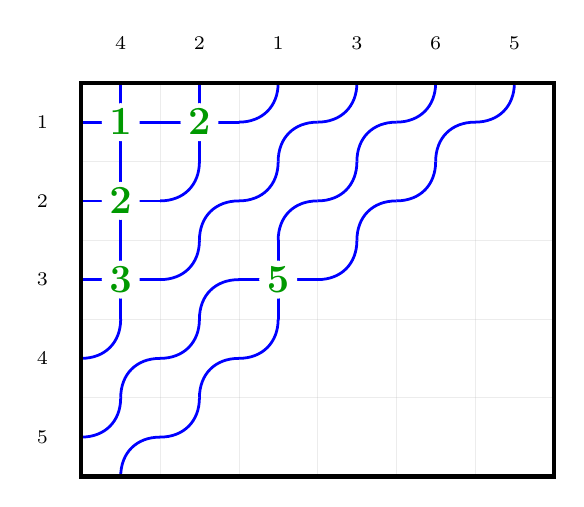
\begin{tikzpicture}[scale=1.0]
  \draw[lightgray, very thin, opacity=0.3] (0,1) -- (6,1);
  \draw[lightgray, very thin, opacity=0.3] (0,2) -- (6,2);
  \draw[lightgray, very thin, opacity=0.3] (0,3) -- (6,3);
  \draw[lightgray, very thin, opacity=0.3] (0,4) -- (6,4);
  \draw[lightgray, very thin, opacity=0.3] (0,5) -- (6,5);
  \draw[lightgray, very thin, opacity=0.3] (0,6) -- (6,6);
  \draw[lightgray, very thin, opacity=0.3] (0,1) -- (0,6);
  \draw[lightgray, very thin, opacity=0.3] (1,1) -- (1,6);
  \draw[lightgray, very thin, opacity=0.3] (2,1) -- (2,6);
  \draw[lightgray, very thin, opacity=0.3] (3,1) -- (3,6);
  \draw[lightgray, very thin, opacity=0.3] (4,1) -- (4,6);
  \draw[lightgray, very thin, opacity=0.3] (5,1) -- (5,6);
  \draw[lightgray, very thin, opacity=0.3] (6,1) -- (6,6);
  \draw[blue, line width=1.0pt, line cap=round] (0,5.5) -- (1,5.5);
  \draw[blue, line width=1.0pt, line cap=round] (0.5,5) -- (0.5,6);
  \draw[blue, line width=1.0pt, line cap=round] (1,5.5) -- (2,5.5);
  \draw[blue, line width=1.0pt, line cap=round] (1.5,5) -- (1.5,6);
  \draw[blue, line width=1.0pt] (2,5.5) .. controls (2.3,5.5) and (2.5,5.7) .. (2.5,6);
  \draw[blue, line width=1.0pt] (2.5,5) .. controls (2.5,5.3) and (2.7,5.5) .. (3,5.5);
  \draw[blue, line width=1.0pt] (3,5.5) .. controls (3.3,5.5) and (3.5,5.7) .. (3.5,6);
  \draw[blue, line width=1.0pt] (3.5,5) .. controls (3.5,5.3) and (3.7,5.5) .. (4,5.5);
  \draw[blue, line width=1.0pt] (4,5.5) .. controls (4.3,5.5) and (4.5,5.7) .. (4.5,6);
  \draw[blue, line width=1.0pt] (4.5,5) .. controls (4.5,5.3) and (4.7,5.5) .. (5,5.5);
  \draw[blue, line width=1.0pt] (5,5.5) .. controls (5.3,5.5) and (5.5,5.7) .. (5.5,6);
  \draw[blue, line width=1.0pt, line cap=round] (0,4.5) -- (1,4.5);
  \draw[blue, line width=1.0pt, line cap=round] (0.5,4) -- (0.5,5);
  \draw[blue, line width=1.0pt] (1,4.5) .. controls (1.3,4.5) and (1.5,4.7) .. (1.5,5);
  \draw[blue, line width=1.0pt] (1.5,4) .. controls (1.5,4.3) and (1.7,4.5) .. (2,4.5);
  \draw[blue, line width=1.0pt] (2,4.5) .. controls (2.3,4.5) and (2.5,4.7) .. (2.5,5);
  \draw[blue, line width=1.0pt] (2.5,4) .. controls (2.5,4.3) and (2.7,4.5) .. (3,4.5);
  \draw[blue, line width=1.0pt] (3,4.5) .. controls (3.3,4.5) and (3.5,4.7) .. (3.5,5);
  \draw[blue, line width=1.0pt] (3.5,4) .. controls (3.5,4.3) and (3.7,4.5) .. (4,4.5);
  \draw[blue, line width=1.0pt] (4,4.5) .. controls (4.3,4.5) and (4.5,4.7) .. (4.5,5);
  \draw[blue, line width=1.0pt, line cap=round] (0,3.5) -- (1,3.5);
  \draw[blue, line width=1.0pt, line cap=round] (0.5,3) -- (0.5,4);
  \draw[blue, line width=1.0pt] (1,3.5) .. controls (1.3,3.5) and (1.5,3.7) .. (1.5,4);
  \draw[blue, line width=1.0pt] (1.5,3) .. controls (1.5,3.3) and (1.7,3.5) .. (2,3.5);
  \draw[blue, line width=1.0pt, line cap=round] (2,3.5) -- (3,3.5);
  \draw[blue, line width=1.0pt, line cap=round] (2.5,3) -- (2.5,4);
  \draw[blue, line width=1.0pt] (3,3.5) .. controls (3.3,3.5) and (3.5,3.7) .. (3.5,4);
  \draw[blue, line width=1.0pt] (0,2.5) .. controls (0.3,2.5) and (0.5,2.7) .. (0.5,3);
  \draw[blue, line width=1.0pt] (0.5,2) .. controls (0.5,2.3) and (0.7,2.5) .. (1,2.5);
  \draw[blue, line width=1.0pt] (1,2.5) .. controls (1.3,2.5) and (1.5,2.7) .. (1.5,3);
  \draw[blue, line width=1.0pt] (1.5,2) .. controls (1.5,2.3) and (1.7,2.5) .. (2,2.5);
  \draw[blue, line width=1.0pt] (2,2.5) .. controls (2.3,2.5) and (2.5,2.7) .. (2.5,3);
  \draw[blue, line width=1.0pt] (0,1.5) .. controls (0.3,1.5) and (0.5,1.7) .. (0.5,2);
  \draw[blue, line width=1.0pt] (0.5,1) .. controls (0.5,1.3) and (0.7,1.5) .. (1,1.5);
  \draw[blue, line width=1.0pt] (1,1.5) .. controls (1.3,1.5) and (1.5,1.7) .. (1.5,2);
  \node[font=\Large\bfseries, text=green!60!black, fill=white, inner sep=0.5pt, circle, transform shape] at (1.5,5.5) {2};
  \node[font=\Large\bfseries, text=green!60!black, fill=white, inner sep=0.5pt, circle, transform shape] at (0.5,4.5) {2};
  \node[font=\Large\bfseries, text=green!60!black, fill=white, inner sep=0.5pt, circle, transform shape] at (0.5,3.5) {3};
  \node[font=\Large\bfseries, text=green!60!black, fill=white, inner sep=0.5pt, circle, transform shape] at (0.5,5.5) {1};
  \node[font=\Large\bfseries, text=green!60!black, fill=white, inner sep=0.5pt, circle, transform shape] at (2.5,3.5) {5};
  \node[font=\scriptsize, text=black, anchor=south] at (0.5,6.3) {4};
  \node[font=\scriptsize, text=black, anchor=south] at (1.5,6.3) {2};
  \node[font=\scriptsize, text=black, anchor=south] at (2.5,6.3) {1};
  \node[font=\scriptsize, text=black, anchor=south] at (3.5,6.3) {3};
  \node[font=\scriptsize, text=black, anchor=south] at (4.5,6.3) {6};
  \node[font=\scriptsize, text=black, anchor=south] at (5.5,6.3) {5};
  \node[font=\scriptsize, text=black, anchor=east] at (-0.3,5.5) {1};
  \node[font=\scriptsize, text=black, anchor=east] at (-0.3,4.5) {2};
  \node[font=\scriptsize, text=black, anchor=east] at (-0.3,3.5) {3};
  \node[font=\scriptsize, text=black, anchor=east] at (-0.3,2.5) {4};
  \node[font=\scriptsize, text=black, anchor=east] at (-0.3,1.5) {5};
  \draw[black, line width=1.5pt] (0,1) rectangle (6,6);
\end{tikzpicture}
\end{figure}


The main benefit of this is that visualizing $\rtt_R(i,j)$ is easy. The pipes that pass through position $(i,j)$ are labeled $s$ and $q$ for some $s,q>0$. For a positive root in an unoccupied square, we will have the following labeling, where $q<s$:

\begin{center}
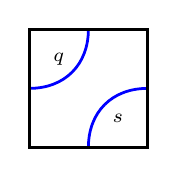
\begin{tikzpicture}[scale=1.5]
  % Draw the grid for a single square
  \draw[lightgray, very thin, opacity=0.3] (0,0) -- (1,0);
  \draw[lightgray, very thin, opacity=0.3] (0,1) -- (1,1);
  \draw[lightgray, very thin, opacity=0.3] (0,0) -- (0,1);
  \draw[lightgray, very thin, opacity=0.3] (1,0) -- (1,1);
  
  % Draw the elbow with two arcs
  % Blue arc (from left to top)
  \draw[blue, line width=1.0pt] (0,0.5) .. controls (0.3,0.5) and (0.5,0.7) .. (0.5,1);
  
  % Red arc (from bottom to right)
  \draw[blue, line width=1.0pt] (0.5,0) .. controls (0.5,0.3) and (0.7,0.5) .. (1,0.5);
  
  % Labels
  \node[font=\scriptsize, text=black] at (0.25,0.75) {$q$};
  \node[font=\scriptsize, text=black] at (0.75,0.25) {$s$};
  
  % Box around the grid
  \draw[black, line width=1.2pt] (0,0) rectangle (1,1);
\end{tikzpicture}
\end{center}

We observe that in the above RC graph, the position $(1,5)$ does not have this configuration. Placing a crossing there would create a negative root, and the pipes would cross twice. \emph{Note that this results in a collection of ordered pairs that is not an RC graph, if such a crossing exists.} For a valid RC graphs, only positive roots occur as crossings, and this happens if and only if pipes cross at most once.

\begin{figure}[h]
\centering
\caption{An invalid set of crossings causing pipes to cross more than once, caused by inserting a crossing at a negative root}
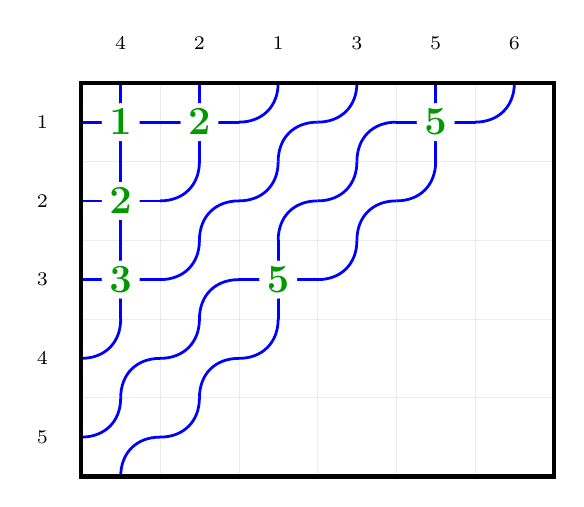
\begin{tikzpicture}[scale=1.0]
  \draw[lightgray, very thin, opacity=0.3] (0,1) -- (6,1);
  \draw[lightgray, very thin, opacity=0.3] (0,2) -- (6,2);
  \draw[lightgray, very thin, opacity=0.3] (0,3) -- (6,3);
  \draw[lightgray, very thin, opacity=0.3] (0,4) -- (6,4);
  \draw[lightgray, very thin, opacity=0.3] (0,5) -- (6,5);
  \draw[lightgray, very thin, opacity=0.3] (0,6) -- (6,6);
  \draw[lightgray, very thin, opacity=0.3] (0,1) -- (0,6);
  \draw[lightgray, very thin, opacity=0.3] (1,1) -- (1,6);
  \draw[lightgray, very thin, opacity=0.3] (2,1) -- (2,6);
  \draw[lightgray, very thin, opacity=0.3] (3,1) -- (3,6);
  \draw[lightgray, very thin, opacity=0.3] (4,1) -- (4,6);
  \draw[lightgray, very thin, opacity=0.3] (5,1) -- (5,6);
  \draw[lightgray, very thin, opacity=0.3] (6,1) -- (6,6);
  \draw[blue, line width=1.0pt, line cap=round] (0,5.5) -- (1,5.5);
  \draw[blue, line width=1.0pt, line cap=round] (0.5,5) -- (0.5,6);
  \draw[blue, line width=1.0pt, line cap=round] (1,5.5) -- (2,5.5);
  \draw[blue, line width=1.0pt, line cap=round] (1.5,5) -- (1.5,6);
  \draw[blue, line width=1.0pt] (2,5.5) .. controls (2.3,5.5) and (2.5,5.7) .. (2.5,6);
  \draw[blue, line width=1.0pt] (2.5,5) .. controls (2.5,5.3) and (2.7,5.5) .. (3,5.5);
  \draw[blue, line width=1.0pt] (3,5.5) .. controls (3.3,5.5) and (3.5,5.7) .. (3.5,6);
  \draw[blue, line width=1.0pt] (3.5,5) .. controls (3.5,5.3) and (3.7,5.5) .. (4,5.5);
  \draw[blue, line width=1.0pt, line cap=round] (4,5.5) -- (5,5.5);
  \draw[blue, line width=1.0pt, line cap=round] (4.5,5) -- (4.5,6);
  \draw[blue, line width=1.0pt] (5,5.5) .. controls (5.3,5.5) and (5.5,5.7) .. (5.5,6);
  \draw[blue, line width=1.0pt, line cap=round] (0,4.5) -- (1,4.5);
  \draw[blue, line width=1.0pt, line cap=round] (0.5,4) -- (0.5,5);
  \draw[blue, line width=1.0pt] (1,4.5) .. controls (1.3,4.5) and (1.5,4.7) .. (1.5,5);
  \draw[blue, line width=1.0pt] (1.5,4) .. controls (1.5,4.3) and (1.7,4.5) .. (2,4.5);
  \draw[blue, line width=1.0pt] (2,4.5) .. controls (2.3,4.5) and (2.5,4.7) .. (2.5,5);
  \draw[blue, line width=1.0pt] (2.5,4) .. controls (2.5,4.3) and (2.7,4.5) .. (3,4.5);
  \draw[blue, line width=1.0pt] (3,4.5) .. controls (3.3,4.5) and (3.5,4.7) .. (3.5,5);
  \draw[blue, line width=1.0pt] (3.5,4) .. controls (3.5,4.3) and (3.7,4.5) .. (4,4.5);
  \draw[blue, line width=1.0pt] (4,4.5) .. controls (4.3,4.5) and (4.5,4.7) .. (4.5,5);
  \draw[blue, line width=1.0pt, line cap=round] (0,3.5) -- (1,3.5);
  \draw[blue, line width=1.0pt, line cap=round] (0.5,3) -- (0.5,4);
  \draw[blue, line width=1.0pt] (1,3.5) .. controls (1.3,3.5) and (1.5,3.7) .. (1.5,4);
  \draw[blue, line width=1.0pt] (1.5,3) .. controls (1.5,3.3) and (1.7,3.5) .. (2,3.5);
  \draw[blue, line width=1.0pt, line cap=round] (2,3.5) -- (3,3.5);
  \draw[blue, line width=1.0pt, line cap=round] (2.5,3) -- (2.5,4);
  \draw[blue, line width=1.0pt] (3,3.5) .. controls (3.3,3.5) and (3.5,3.7) .. (3.5,4);
  \draw[blue, line width=1.0pt] (0,2.5) .. controls (0.3,2.5) and (0.5,2.7) .. (0.5,3);
  \draw[blue, line width=1.0pt] (0.5,2) .. controls (0.5,2.3) and (0.7,2.5) .. (1,2.5);
  \draw[blue, line width=1.0pt] (1,2.5) .. controls (1.3,2.5) and (1.5,2.7) .. (1.5,3);
  \draw[blue, line width=1.0pt] (1.5,2) .. controls (1.5,2.3) and (1.7,2.5) .. (2,2.5);
  \draw[blue, line width=1.0pt] (2,2.5) .. controls (2.3,2.5) and (2.5,2.7) .. (2.5,3);
  \draw[blue, line width=1.0pt] (0,1.5) .. controls (0.3,1.5) and (0.5,1.7) .. (0.5,2);
  \draw[blue, line width=1.0pt] (0.5,1) .. controls (0.5,1.3) and (0.7,1.5) .. (1,1.5);
  \draw[blue, line width=1.0pt] (1,1.5) .. controls (1.3,1.5) and (1.5,1.7) .. (1.5,2);
  \node[font=\Large\bfseries, text=green!60!black, fill=white, inner sep=0.5pt, circle, transform shape] at (1.5,5.5) {2};
  \node[font=\Large\bfseries, text=green!60!black, fill=white, inner sep=0.5pt, circle, transform shape] at (0.5,4.5) {2};
  \node[font=\Large\bfseries, text=green!60!black, fill=white, inner sep=0.5pt, circle, transform shape] at (4.5,5.5) {5};
  \node[font=\Large\bfseries, text=green!60!black, fill=white, inner sep=0.5pt, circle, transform shape] at (0.5,3.5) {3};
  \node[font=\Large\bfseries, text=green!60!black, fill=white, inner sep=0.5pt, circle, transform shape] at (0.5,5.5) {1};
  \node[font=\Large\bfseries, text=green!60!black, fill=white, inner sep=0.5pt, circle, transform shape] at (2.5,3.5) {5};
  \node[font=\scriptsize, text=black, anchor=south] at (0.5,6.3) {4};
  \node[font=\scriptsize, text=black, anchor=south] at (1.5,6.3) {2};
  \node[font=\scriptsize, text=black, anchor=south] at (2.5,6.3) {1};
  \node[font=\scriptsize, text=black, anchor=south] at (3.5,6.3) {3};
  \node[font=\scriptsize, text=black, anchor=south] at (4.5,6.3) {5};
  \node[font=\scriptsize, text=black, anchor=south] at (5.5,6.3) {6};
  \node[font=\scriptsize, text=black, anchor=east] at (-0.3,5.5) {1};
  \node[font=\scriptsize, text=black, anchor=east] at (-0.3,4.5) {2};
  \node[font=\scriptsize, text=black, anchor=east] at (-0.3,3.5) {3};
  \node[font=\scriptsize, text=black, anchor=east] at (-0.3,2.5) {4};
  \node[font=\scriptsize, text=black, anchor=east] at (-0.3,1.5) {5};
  \draw[black, line width=1.5pt] (0,1) rectangle (6,6);
\end{tikzpicture}
\end{figure}

\subsection{Zeroing out the last row}

We proceed now to define a product on $\BRC$ turning it into a ring. To do this, we need to be able to define a function $\zeromap:\BRC\to\BRC$ trimming empty rows from the bottom instead of from the top. This is far more complicated.


\newcommand{\xleadsto}[2][]{\overset{#2}{\leadsto}}

\newcommand{\ins}[2]{{#2\xleadsto{#1}}}

\begin{algorithm}
\caption{Basic monk insertion $\ins{k}{i} R$}
\label{algorithm:monk}
\begin{algorithmic}[1]
		\State \textbf{Input:} An RC graph $R$, parameter $k$, and an integer $i$ with $1\leq i\leq k$.
		\State \textbf{Output:} A modified RC graph $R'$ with $\wtt_j(R')=\wtt_j(R)$  for $j\neq i$ and $\wtt_i(R')=\wtt_i(R)+1$ such that $\wof{R}\tom{k} \wof{R'}$.
		\State Find leftmost position $(i, j) \notin R$ in row $i$ such that if $\rtt_R(i, j)=(a,b)$, then $a\leq k < b$.
		\State $R \gets R \cup \{(i, j)\}$
    \If{there exists $(i', j') \in R$ with $\rtt_R(i', j') \in \Phi^-$}
        \State $R \gets R \setminus \{(i', j')\}$
        \State Return to step 3 substituting $i = i'$.
    \EndIf
		\State \Return $R$
	\end{algorithmic}
\end{algorithm}

\begin{algorithm} 
	\caption{Pseudo-Pieri insertion $\ins{k}{I} R$}
	\label{algorithm:insertion}
	\begin{algorithmic}[1]
		\State \textbf{Input:} An RC graph $R$, parameter $k$, and sequence $I = \{i_1, \ldots, i_m\}$ with $k\geq i_1 \geq i_2 \geq \cdots \geq i_m \geq 1$.
		\State \textbf{Output:} A modified RC graph $R'$ with $\wtt_i(R')=\wtt_i(R)$ for $i\notin I$ and $\wtt_i(R')=\wtt_i(R)+\#\{j \mid i_j = i\}$ for $i\in I$ such that $\wof{R}\Tom{k} \wof{R'}$.
		\State \textbf{Initialize:} Let $L \gets [\,]$ (empty list of pairs $(a, b)$ where $a \leq k < b$), and $U\gets [\,]$ (empty list of positions).
		\For{each $i \in (i_1, \ldots, i_m)$}
		\State Find leftmost position $(i, j) \notin R$ in row $i$ satisfying $j>j'$ for all $(i,j')\in U$ such that either:
		\State \quad a) $\rtt_R(i, j) = (s, q)$ where $s \leq k < q$ and $q \notin \{b \mid (a, b) \in L\}$.
		\State \quad b) $\rtt_R(i, j) = (b_r, q)$ where $q > k$, $b_r<q$, and $q \notin \{b \mid (a, b) \in L\}$.
		\State $R \gets R \cup \{(i, j)\}$ and $U\gets U \cup \{(i, j)\}$
		\State Update $L$ by adding $(s, q)$ or replacing $(a_r, b_r)$ with $(a_r, q)$ and $(a_r, b_r)$.
		\If{there exists $(i', j') \in R$ with $\rtt_R(i', j') \in \Phi^-$}
        
    \State $R \gets R \setminus \{(i', j')\}$
		\State Let $\rtt_R(i', j') = (q, s)$
		\If{$(s, q) \in L$}
		\State Remove $(s, q)$ from $L$
		\Else
		\State Remove $(a_r, q)$ from $L$, where $(a_r, q),(a_r,s)\in L$
		\EndIf
		\State Return to step 5 to insert $i'$.
    \EndIf
		\EndFor
		\State \Return $R$
	\end{algorithmic}
\end{algorithm}


\begin{algorithm} 
	\caption{Map $\zeromap(R)$ zeroing out last row}
	\label{algorithm:zero}
	\begin{algorithmic}[1]
		\State \textbf{Input:} A bounded RC graph $R$ with $\hr(R)=n$ and row $n$ empty.
		\State \textbf{Output:} A bounded RC graph $R'$ with $\hr(R')=n-1$, $|R'|=|R|$ (same number of crossings), and $\wof{R}\downvar{n} \wof{R'}$.
		
		\If{$R$ with last row removed is a valid bounded RC graph}
		\State \Return $R$ with last row removed
		\Else
		\State Let $R_0 \gets R$.
		\State Find the maximal $p$ and sequence $\{(i_m, j_m)\}_{m=1}^p$ such that:
		\State \quad $\rtt_{R_{m-1}}(i_m, j_m) = (n+m-1,n+m)$ for each $m$, where $R_m = R_{m-1}\setminus\{(i_m, j_m)\}$ for each $m\geq 1$.
		\State $R^- \gets R \setminus \{(i_1, j_1), \ldots, (i_p, j_p)\}$.
		\State Let $I \gets (i_1, i_2, \ldots, i_p)$.
		\State $D \gets R^- \cup \{(n, 1), (n, 2), \ldots, (n, p)\}$.
		\State $D' \gets \ins{n-1}{I} D$
		\State $R' \gets \{(i, j) \in D' \mid i < n\}$ as a bounded RC graph with $n-1$ rows.
		\State \Return $R'$.
		\EndIf
	\end{algorithmic}
\end{algorithm}

See Figure \ref{fig:zeroing} for an example of the zeroing operation (Algorithm \ref{algorithm:zero}). 

\def\multiset#1#2{\ensuremath{\left(\kern-.3em\left(\genfrac{}{}{0pt}{}{#1}{#2}\right)\kern-.3em\right)}}


Note that Algorithm \ref{algorithm:insertion} is \emph{not} a realization of Sottile's Pieri formula for complete symmetric polynomials, despite preserving the relevant Bruhat relation. This is because the map 
$$\multiset{k}{p}\times\RC(w)\to \RC(n)$$
given by 
$$(I, R)\mapsto \ins{k}{I} R$$ 
need not be injective.

\begin{definition}\label{definition:zeromap}
Let $R$ be an RC graph with $\hr(R) = n$ such that row $n$ is empty. We define $\zeromap(R)$ to be the output of Algorithm \ref{algorithm:zero}, an RC graph with $n-1$ rows, on input $R$.
\end{definition}

\begin{figure}[htbp]
\centering

% First diagram
\begin{minipage}{0.45\textwidth}
\centering
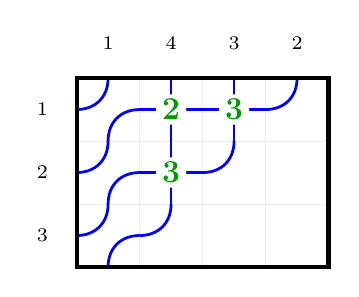
\begin{tikzpicture}[scale=0.8]
  \draw[lightgray, very thin, opacity=0.3] (0,1) -- (4,1);
  \draw[lightgray, very thin, opacity=0.3] (0,2) -- (4,2);
  \draw[lightgray, very thin, opacity=0.3] (0,3) -- (4,3);
  \draw[lightgray, very thin, opacity=0.3] (0,4) -- (4,4);
  \draw[lightgray, very thin, opacity=0.3] (0,1) -- (0,4);
  \draw[lightgray, very thin, opacity=0.3] (1,1) -- (1,4);
  \draw[lightgray, very thin, opacity=0.3] (2,1) -- (2,4);
  \draw[lightgray, very thin, opacity=0.3] (3,1) -- (3,4);
  \draw[lightgray, very thin, opacity=0.3] (4,1) -- (4,4);
  \draw[blue, line width=1.0pt] (0,3.5) .. controls (0.3,3.5) and (0.5,3.7) .. (0.5,4);
  \draw[blue, line width=1.0pt] (0.5,3) .. controls (0.5,3.3) and (0.7,3.5) .. (1,3.5);
  \draw[blue, line width=1.0pt, line cap=round] (1,3.5) -- (2,3.5);
  \draw[blue, line width=1.0pt, line cap=round] (1.5,3) -- (1.5,4);
  \draw[blue, line width=1.0pt, line cap=round] (2,3.5) -- (3,3.5);
  \draw[blue, line width=1.0pt, line cap=round] (2.5,3) -- (2.5,4);
  \draw[blue, line width=1.0pt] (3,3.5) .. controls (3.3,3.5) and (3.5,3.7) .. (3.5,4);
  \draw[blue, line width=1.0pt] (0,2.5) .. controls (0.3,2.5) and (0.5,2.7) .. (0.5,3);
  \draw[blue, line width=1.0pt] (0.5,2) .. controls (0.5,2.3) and (0.7,2.5) .. (1,2.5);
  \draw[blue, line width=1.0pt, line cap=round] (1,2.5) -- (2,2.5);
  \draw[blue, line width=1.0pt, line cap=round] (1.5,2) -- (1.5,3);
  \draw[blue, line width=1.0pt] (2,2.5) .. controls (2.3,2.5) and (2.5,2.7) .. (2.5,3);
  \draw[blue, line width=1.0pt] (0,1.5) .. controls (0.3,1.5) and (0.5,1.7) .. (0.5,2);
  \draw[blue, line width=1.0pt] (0.5,1) .. controls (0.5,1.3) and (0.7,1.5) .. (1,1.5);
  \draw[blue, line width=1.0pt] (1,1.5) .. controls (1.3,1.5) and (1.5,1.7) .. (1.5,2);
  \node[font=\Large\bfseries, text=green!60!black, fill=white, inner sep=0.5pt, circle, transform shape] at (1.5,3.5) {2};
  \node[font=\Large\bfseries, text=green!60!black, fill=white, inner sep=0.5pt, circle, transform shape] at (2.5,3.5) {3};
  \node[font=\Large\bfseries, text=green!60!black, fill=white, inner sep=0.5pt, circle, transform shape] at (1.5,2.5) {3};
  \node[font=\scriptsize, text=black, anchor=south] at (0.5,4.3) {1};
  \node[font=\scriptsize, text=black, anchor=south] at (1.5,4.3) {4};
  \node[font=\scriptsize, text=black, anchor=south] at (2.5,4.3) {3};
  \node[font=\scriptsize, text=black, anchor=south] at (3.5,4.3) {2};
  \node[font=\scriptsize, text=black, anchor=east] at (-0.3,3.5) {1};
  \node[font=\scriptsize, text=black, anchor=east] at (-0.3,2.5) {2};
  \node[font=\scriptsize, text=black, anchor=east] at (-0.3,1.5) {3};
  \draw[black, line width=1.5pt] (0,1) rectangle (4,4);
\end{tikzpicture}
\caption*{(a) Initial RC graph $R$}
\end{minipage}
\hfill
% Second diagram
\begin{minipage}{0.45\textwidth}
\centering
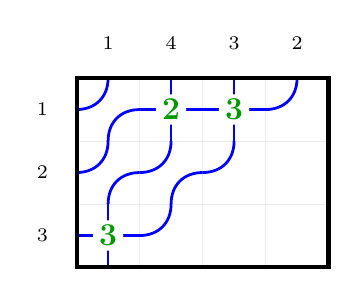
\begin{tikzpicture}[scale=0.8]
  \draw[lightgray, very thin, opacity=0.3] (0,1) -- (4,1);
  \draw[lightgray, very thin, opacity=0.3] (0,2) -- (4,2);
  \draw[lightgray, very thin, opacity=0.3] (0,3) -- (4,3);
  \draw[lightgray, very thin, opacity=0.3] (0,4) -- (4,4);
  \draw[lightgray, very thin, opacity=0.3] (0,1) -- (0,4);
  \draw[lightgray, very thin, opacity=0.3] (1,1) -- (1,4);
  \draw[lightgray, very thin, opacity=0.3] (2,1) -- (2,4);
  \draw[lightgray, very thin, opacity=0.3] (3,1) -- (3,4);
  \draw[lightgray, very thin, opacity=0.3] (4,1) -- (4,4);
  \draw[blue, line width=1.0pt] (0,3.5) .. controls (0.3,3.5) and (0.5,3.7) .. (0.5,4);
  \draw[blue, line width=1.0pt] (0.5,3) .. controls (0.5,3.3) and (0.7,3.5) .. (1,3.5);
  \draw[blue, line width=1.0pt, line cap=round] (1,3.5) -- (2,3.5);
  \draw[blue, line width=1.0pt, line cap=round] (1.5,3) -- (1.5,4);
  \draw[blue, line width=1.0pt, line cap=round] (2,3.5) -- (3,3.5);
  \draw[blue, line width=1.0pt, line cap=round] (2.5,3) -- (2.5,4);
  \draw[blue, line width=1.0pt] (3,3.5) .. controls (3.3,3.5) and (3.5,3.7) .. (3.5,4);
  \draw[blue, line width=1.0pt] (0,2.5) .. controls (0.3,2.5) and (0.5,2.7) .. (0.5,3);
  \draw[blue, line width=1.0pt] (0.5,2) .. controls (0.5,2.3) and (0.7,2.5) .. (1,2.5);
  \draw[blue, line width=1.0pt] (1,2.5) .. controls (1.3,2.5) and (1.5,2.7) .. (1.5,3);
  \draw[blue, line width=1.0pt] (1.5,2) .. controls (1.5,2.3) and (1.7,2.5) .. (2,2.5);
  \draw[blue, line width=1.0pt] (2,2.5) .. controls (2.3,2.5) and (2.5,2.7) .. (2.5,3);
  \draw[blue, line width=1.0pt, line cap=round] (0,1.5) -- (1,1.5);
  \draw[blue, line width=1.0pt, line cap=round] (0.5,1) -- (0.5,2);
  \draw[blue, line width=1.0pt] (1,1.5) .. controls (1.3,1.5) and (1.5,1.7) .. (1.5,2);
  \node[font=\Large\bfseries, text=green!60!black, fill=white, inner sep=0.5pt, circle, transform shape] at (0.5,1.5) {3};
  \node[font=\Large\bfseries, text=green!60!black, fill=white, inner sep=0.5pt, circle, transform shape] at (1.5,3.5) {2};
  \node[font=\Large\bfseries, text=green!60!black, fill=white, inner sep=0.5pt, circle, transform shape] at (2.5,3.5) {3};
  \node[font=\scriptsize, text=black, anchor=south] at (0.5,4.3) {1};
  \node[font=\scriptsize, text=black, anchor=south] at (1.5,4.3) {4};
  \node[font=\scriptsize, text=black, anchor=south] at (2.5,4.3) {3};
  \node[font=\scriptsize, text=black, anchor=south] at (3.5,4.3) {2};
  \node[font=\scriptsize, text=black, anchor=east] at (-0.3,3.5) {1};
  \node[font=\scriptsize, text=black, anchor=east] at (-0.3,2.5) {2};
  \node[font=\scriptsize, text=black, anchor=east] at (-0.3,1.5) {3};
  \draw[black, line width=1.5pt] (0,1) rectangle (4,4);
\end{tikzpicture}
\caption*{(b) After deleting $(2,2)$ with $\rtt_R(2,2)=\alpha_3$ and moving to row $3$}
\end{minipage}

\vspace{1em}

% Third diagram
\begin{minipage}{0.45\textwidth}
\centering
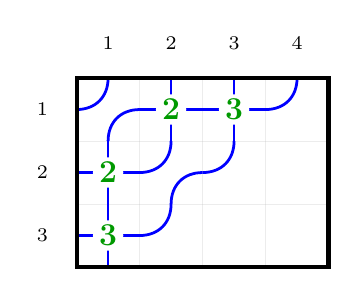
\begin{tikzpicture}[scale=0.8]
  \draw[lightgray, very thin, opacity=0.3] (0,1) -- (4,1);
  \draw[lightgray, very thin, opacity=0.3] (0,2) -- (4,2);
  \draw[lightgray, very thin, opacity=0.3] (0,3) -- (4,3);
  \draw[lightgray, very thin, opacity=0.3] (0,4) -- (4,4);
  \draw[lightgray, very thin, opacity=0.3] (0,1) -- (0,4);
  \draw[lightgray, very thin, opacity=0.3] (1,1) -- (1,4);
  \draw[lightgray, very thin, opacity=0.3] (2,1) -- (2,4);
  \draw[lightgray, very thin, opacity=0.3] (3,1) -- (3,4);
  \draw[lightgray, very thin, opacity=0.3] (4,1) -- (4,4);
  \draw[blue, line width=1.0pt] (0,3.5) .. controls (0.3,3.5) and (0.5,3.7) .. (0.5,4);
  \draw[blue, line width=1.0pt] (0.5,3) .. controls (0.5,3.3) and (0.7,3.5) .. (1,3.5);
  \draw[blue, line width=1.0pt, line cap=round] (1,3.5) -- (2,3.5);
  \draw[blue, line width=1.0pt, line cap=round] (1.5,3) -- (1.5,4);
  \draw[blue, line width=1.0pt, line cap=round] (2,3.5) -- (3,3.5);
  \draw[blue, line width=1.0pt, line cap=round] (2.5,3) -- (2.5,4);
  \draw[blue, line width=1.0pt] (3,3.5) .. controls (3.3,3.5) and (3.5,3.7) .. (3.5,4);
  \draw[blue, line width=1.0pt, line cap=round] (0,2.5) -- (1,2.5);
  \draw[blue, line width=1.0pt, line cap=round] (0.5,2) -- (0.5,3);
  \draw[blue, line width=1.0pt] (1,2.5) .. controls (1.3,2.5) and (1.5,2.7) .. (1.5,3);
  \draw[blue, line width=1.0pt] (1.5,2) .. controls (1.5,2.3) and (1.7,2.5) .. (2,2.5);
  \draw[blue, line width=1.0pt] (2,2.5) .. controls (2.3,2.5) and (2.5,2.7) .. (2.5,3);
  \draw[blue, line width=1.0pt, line cap=round] (0,1.5) -- (1,1.5);
  \draw[blue, line width=1.0pt, line cap=round] (0.5,1) -- (0.5,2);
  \draw[blue, line width=1.0pt] (1,1.5) .. controls (1.3,1.5) and (1.5,1.7) .. (1.5,2);
  \node[font=\Large\bfseries, text=green!60!black, fill=white, inner sep=0.5pt, circle, transform shape] at (0.5,1.5) {3};
  \node[font=\Large\bfseries, text=green!60!black, fill=white, inner sep=0.5pt, circle, transform shape] at (1.5,3.5) {2};
  \node[font=\Large\bfseries, text=green!60!black, fill=white, inner sep=0.5pt, circle, transform shape] at (2.5,3.5) {3};
  \node[font=\Large\bfseries, text=green!60!black, fill=white, inner sep=0.5pt, circle, transform shape] at (0.5,2.5) {2};
  \node[font=\scriptsize, text=black, anchor=south] at (0.5,4.3) {1};
  \node[font=\scriptsize, text=black, anchor=south] at (1.5,4.3) {2};
  \node[font=\scriptsize, text=black, anchor=south] at (2.5,4.3) {3};
  \node[font=\scriptsize, text=black, anchor=south] at (3.5,4.3) {4};
  \node[font=\scriptsize, text=black, anchor=east] at (-0.3,3.5) {1};
  \node[font=\scriptsize, text=black, anchor=east] at (-0.3,2.5) {2};
  \node[font=\scriptsize, text=black, anchor=east] at (-0.3,1.5) {3};
  \draw[black, line width=1.5pt] (0,1) rectangle (4,4);
\end{tikzpicture}
\caption*{(c) After insertion with $i_1=2$}
\end{minipage}
\hfill
% Fourth diagram
\begin{minipage}{0.45\textwidth}
\centering
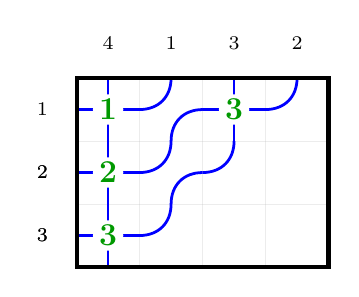
\begin{tikzpicture}[scale=0.8]
  \draw[lightgray, very thin, opacity=0.3] (0,1) -- (4,1);
  \draw[lightgray, very thin, opacity=0.3] (0,2) -- (4,2);
  \draw[lightgray, very thin, opacity=0.3] (0,3) -- (4,3);
  \draw[lightgray, very thin, opacity=0.3] (0,4) -- (4,4);
  \draw[lightgray, very thin, opacity=0.3] (0,1) -- (0,4);
  \draw[lightgray, very thin, opacity=0.3] (1,1) -- (1,4);
  \draw[lightgray, very thin, opacity=0.3] (2,1) -- (2,4);
  \draw[lightgray, very thin, opacity=0.3] (3,1) -- (3,4);
  \draw[lightgray, very thin, opacity=0.3] (4,1) -- (4,4);
  \draw[blue, line width=1.0pt, line cap=round] (0,3.5) -- (1,3.5);
  \draw[blue, line width=1.0pt, line cap=round] (0.5,3) -- (0.5,4);
  \draw[blue, line width=1.0pt] (1,3.5) .. controls (1.3,3.5) and (1.5,3.7) .. (1.5,4);
  \draw[blue, line width=1.0pt] (1.5,3) .. controls (1.5,3.3) and (1.7,3.5) .. (2,3.5);
  \draw[blue, line width=1.0pt, line cap=round] (2,3.5) -- (3,3.5);
  \draw[blue, line width=1.0pt, line cap=round] (2.5,3) -- (2.5,4);
  \draw[blue, line width=1.0pt] (3,3.5) .. controls (3.3,3.5) and (3.5,3.7) .. (3.5,4);
  \draw[blue, line width=1.0pt, line cap=round] (0,2.5) -- (1,2.5);
  \draw[blue, line width=1.0pt, line cap=round] (0.5,2) -- (0.5,3);
  \draw[blue, line width=1.0pt] (1,2.5) .. controls (1.3,2.5) and (1.5,2.7) .. (1.5,3);
  \draw[blue, line width=1.0pt] (1.5,2) .. controls (1.5,2.3) and (1.7,2.5) .. (2,2.5);
  \draw[blue, line width=1.0pt] (2,2.5) .. controls (2.3,2.5) and (2.5,2.7) .. (2.5,3);
  \draw[blue, line width=1.0pt, line cap=round] (0,1.5) -- (1,1.5);
  \draw[blue, line width=1.0pt, line cap=round] (0.5,1) -- (0.5,2);
  \draw[blue, line width=1.0pt] (1,1.5) .. controls (1.3,1.5) and (1.5,1.7) .. (1.5,2);
  \node[font=\Large\bfseries, text=green!60!black, fill=white, inner sep=0.5pt, circle, transform shape] at (0.5,1.5) {3};
  \node[font=\Large\bfseries, text=green!60!black, fill=white, inner sep=0.5pt, circle, transform shape] at (0.5,3.5) {1};
  \node[font=\Large\bfseries, text=green!60!black, fill=white, inner sep=0.5pt, circle, transform shape] at (2.5,3.5) {3};
  \node[font=\Large\bfseries, text=green!60!black, fill=white, inner sep=0.5pt, circle, transform shape] at (0.5,2.5) {2};
  \node[font=\scriptsize, text=black, anchor=south] at (0.5,4.3) {4};
  \node[font=\scriptsize, text=black, anchor=south] at (1.5,4.3) {1};
  \node[font=\scriptsize, text=black, anchor=south] at (2.5,4.3) {3};
  \node[font=\scriptsize, text=black, anchor=south] at (3.5,4.3) {2};
  \node[font=\scriptsize, text=black, anchor=east] at (-0.3,3.5) {1};
  \node[font=\scriptsize, text=black, anchor=east] at (-0.3,2.5) {2};
  \node[font=\scriptsize, text=black, anchor=east] at (-0.3,1.5) {3};
  \node[font=\scriptsize, text=black, anchor=east] at (-0.3,2.5) {2};
  \node[font=\scriptsize, text=black, anchor=east] at (-0.3,1.5) {3};
  \draw[black, line width=1.5pt] (0,1) rectangle (4,4);
\end{tikzpicture}
\caption*{(d) After rectification}
\end{minipage}

\vspace{1em}

% Fifth diagram
\begin{minipage}{0.45\textwidth}
\centering
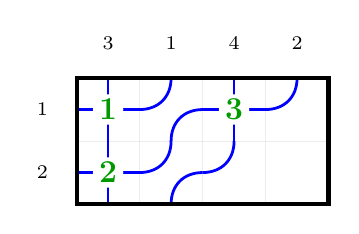
\begin{tikzpicture}[scale=0.8]
  \draw[lightgray, very thin, opacity=0.3] (0,2) -- (4,2);
  \draw[lightgray, very thin, opacity=0.3] (0,3) -- (4,3);
  \draw[lightgray, very thin, opacity=0.3] (0,4) -- (4,4);
  \draw[lightgray, very thin, opacity=0.3] (0,2) -- (0,4);
  \draw[lightgray, very thin, opacity=0.3] (1,2) -- (1,4);
  \draw[lightgray, very thin, opacity=0.3] (2,2) -- (2,4);
  \draw[lightgray, very thin, opacity=0.3] (3,2) -- (3,4);
  \draw[lightgray, very thin, opacity=0.3] (4,2) -- (4,4);
  \draw[blue, line width=1.0pt, line cap=round] (0,3.5) -- (1,3.5);
  \draw[blue, line width=1.0pt, line cap=round] (0.5,3) -- (0.5,4);
  \draw[blue, line width=1.0pt] (1,3.5) .. controls (1.3,3.5) and (1.5,3.7) .. (1.5,4);
  \draw[blue, line width=1.0pt] (1.5,3) .. controls (1.5,3.3) and (1.7,3.5) .. (2,3.5);
  \draw[blue, line width=1.0pt, line cap=round] (2,3.5) -- (3,3.5);
  \draw[blue, line width=1.0pt, line cap=round] (2.5,3) -- (2.5,4);
  \draw[blue, line width=1.0pt] (3,3.5) .. controls (3.3,3.5) and (3.5,3.7) .. (3.5,4);
  \draw[blue, line width=1.0pt, line cap=round] (0,2.5) -- (1,2.5);
  \draw[blue, line width=1.0pt, line cap=round] (0.5,2) -- (0.5,3);
  \draw[blue, line width=1.0pt] (1,2.5) .. controls (1.3,2.5) and (1.5,2.7) .. (1.5,3);
  \draw[blue, line width=1.0pt] (1.5,2) .. controls (1.5,2.3) and (1.7,2.5) .. (2,2.5);
  \draw[blue, line width=1.0pt] (2,2.5) .. controls (2.3,2.5) and (2.5,2.7) .. (2.5,3);
  \node[font=\Large\bfseries, text=green!60!black, fill=white, inner sep=0.5pt, circle, transform shape] at (0.5,3.5) {1};
  \node[font=\Large\bfseries, text=green!60!black, fill=white, inner sep=0.5pt, circle, transform shape] at (2.5,3.5) {3};
  \node[font=\Large\bfseries, text=green!60!black, fill=white, inner sep=0.5pt, circle, transform shape] at (0.5,2.5) {2};
  \node[font=\scriptsize, text=black, anchor=south] at (0.5,4.3) {3};
  \node[font=\scriptsize, text=black, anchor=south] at (1.5,4.3) {1};
  \node[font=\scriptsize, text=black, anchor=south] at (2.5,4.3) {4};
  \node[font=\scriptsize, text=black, anchor=south] at (3.5,4.3) {2};
  \node[font=\scriptsize, text=black, anchor=east] at (-0.3,3.5) {1};
  \node[font=\scriptsize, text=black, anchor=east] at (-0.3,2.5) {2};
  \draw[black, line width=1.5pt] (0,2) rectangle (4,4);
\end{tikzpicture}
\caption*{(e) Final result $\zeromap(R)=(R',2)$ after removing row 3}
\end{minipage}

\caption{Step-by-step computation of $\zeromap(R)$ for $R=\{(1,2),(1,3),(2,2)\}$.}
\label{fig:zeroing}
\end{figure}



\begin{lemma} \label{lemma:insertworks}
Given an RC graph $R$, an integer $k$, and $k\geq i_1\geq\cdots\geq i_m\geq 1$, Algorithm \ref{algorithm:insertion} produces a valid RC graph $R'$ satisfying
$$\wtt_i(R') = \wtt_i(R) + \#\{j \mid i_j = i\}$$
and
$$\wof{R}\Tom{k} \wof{R'}$$
\end{lemma}
\begin{proof}
Set $R_0=R$ to be the initial RC graph. We claim that given $R$ and $L$ at the start of iteration $p$ of the main loop, we have that $R$ is a valid RC graph satisfying
$$\wtt_i(R) = \wtt_i(R_0) + \#\{j \leq p-1 \mid i_j = i\}$$
and
$$\wof{R} = \wof{R_0}t_{a_1b_1}\cdots t_{a_{p-1}b_{p-1}}$$
where $L=[(a_1,b_1),\ldots,(a_p,b_p)]$. This is clear for $p=1$. For larger $p$, suppose we are inserting at row $i_p$. If we are in case (a) of Step 5, then adding $(i_p,j)$ to $R$ adds the root $t_s - t_q$ to the inversion set of $\wof{R}$, and multiplying by $t_{sq}$ gives the desired result. If we are in case (b) of Step 5, then adding $(i_p,j)$ to $R$ results in multiplication by $t_{b_rq}$. This commutes past the other reflections to meet $t_{a_rb_r}$. We thus have the situation
$$t_{a_rb_r}t_{b_rq} = t_{a_rq}t_{a_rb_r}$$
This ensures that the product remains as desired if the RC graph is valid. However, the condition that the RC graph $R$ be valid is not guaranteed after this step, so we must rectify. Suppose we must rectify at row $i - 1$. We find a negative root $(i-1, j')$ which must have been created by the insertion, and hence by the strong exchange property equal to $\rtt_R(i, j)$ that was inserted. Removing this root (from both the graph and from $L$) returns us to the original permutation at the beginning of the iteration, and performing the insert at row $i-1$ adds a new positive root, giving the desired result on the permutation. The weight is unchanged since we removed and added one crossing in row $i-1$. If the algorithm ends here, we have instead multiplied by the new reflection obtained in the ultimate insert step. Otherwise, repeating this process for all necessary rectifications completes the proof of the claim. The claim iterated to $p=m+1$ yields the desired result, and the method of updating $L$ ensures that the $b_j$ are all distinct, so that $\wof{R}\Tom{k} \wof{R'}$.
\end{proof}


\begin{lemma} \label{lemma:zeroweight}
Given a bounded RC graph $R$ with $\hr(R)=n$ such that row $n$ is empty, Algorithm \ref{algorithm:zero} produces a valid bounded RC graph $R'$ with $\hr(R')=n-1$ satisfying
$$\wtt(R') = \wtt(R)$$
\end{lemma}
\begin{proof}
	Stripping out the crossings at roots $(n, n+1), (n+1, n+2), \ldots, (n + p - 1, n + p)$ removes exactly one crossing from each of rows $i_1, i_2, \ldots, i_p$, and moving them to the last row to obtain $R_1$ ensures that $\wof{R}=\wof{R_1}$. By construction, the portion of the RC graph in rows with index less than $n$ is valid (meaning its max descent is at most $n-1$). Applying Algorithm \ref{algorithm:insertion} to insert at rows $i_1, i_2, \ldots, i_p$ adds different crossings to preserve the number of elements in each row without adding descents past index $n$ in the permutation, by Lemma \ref{lemma:insertworks}. Removing row $n$ then yields a valid bounded RC graph $R'$ with $|R'|=n-1$ and the desired properties. 
\end{proof}



\begin{theorem} \label{theorem:zero_bijection}
Let $w$ be a permutation with last descent at most $n$. Let $\mathcal{RC}(w,n)^0$ be the set of bounded RC graphs $R$ with $\hr(R)=n$ such that $\wof{R}=w$ and row $n$ is empty. Then
$$\zeromap:\mathcal{RC}(w, n)^{0}\to \bigcup_{\substack{w\downvar{n} w'\\\ell(w')=\ell(w)}}\mathcal{RC}(w', n-1)$$
is a weight-preserving bijection.
\end{theorem}

To prove Theorem \ref{theorem:zero_bijection} for $n=2$, we may characterize the bounded RC graphs $R$ with $|R|=2$ such that row $2$ is empty and $\maxd(\wof{R})=2$ as those for permutations $w=s_k s_{k-1}\cdots s_2$ for some $k>1$. Algorithm \ref{algorithm:zero} in this case moves the entirety of the crossings in row $1$ to row $2$. The procedure then inserts $k-1$ crossings into row $1$ in order from left to right, which must have roots $t_q - t_s$ such that $q=1$. Thus $R'$ is precisely $\{(1,1), (1,2), (1,3), \ldots, (1, k-1)\}$, which is the unique bounded RC graph for the permutation $w' = s_{k-1} s_{k-2}\cdots s_1$ with one row. This establishes the base case.

For the induction step, we require the following lemmas.

\begin{lemma} \label{lemma:zerotransition}
Let $R$ be a bounded RC graph with $\hr(R)=n\geq 2$ such that row $n$ is empty. Then if $\zeromap(R) = R'$, we have
$$\wof{R}\downvar{n} \wof{R'}$$
\end{lemma}
\begin{proof}
Let $w=\wof{R}$ and suppose $\code_n(w) = m$. By construction, the second to last step of Algorithm \ref{algorithm:zero} yields a bounded RC graph $\widetilde{R}$ with $|\widetilde{R}|=n$ such that if $\widetilde{w} = \wof{\widetilde{R}}$, then
$$\widetilde{w}(n) > \widetilde{w}(n+1) < \widetilde{w}(n+2) < \cdots < \widetilde{w}(n + m)$$
and
$$w\Tom{n-1}\widetilde{w}$$
via reflections $t_{ab}$ such that $n\leq b\leq n+m$. Let $w' = \wof{R'}$. We also have
$$\widetilde{w}\Tom{n}\varphi_{n, N}(w')$$
via only reflections $t_{nb}$ such that $b>n+m$. We claim that
$$w\Tom{n} \varphi_{n, N}(w')$$
This can only fail if $\widetilde{w}(n)\neq w(n)$ by the observations above. However, the pipe labeled $n$, by virtue of the fact that we have $(n,1),\ldots,(n,m)$ populated, will always lie to the right of pipes $n+1,n+2,\ldots,n+m$ in the wiring diagram for $\widetilde{w}$ or any intermediate stage. Inserting into any row that contained a crossing $(n, n+p)$, there must be a valid empty space to the left of the pipe labeled $n$ since we have deleted these crossings. By virtue of the fact that the leftmost is always chosen, no reflection $(i,n)$ will ever be inserted. This ensures that $\widetilde{w}(n) = w(n)$, as desired.
\end{proof}

\begin{corollary} \label{corollary:zerotransition}
  Let $R\in\RC_r(w)^0$ have $\maxd(R)=r$. Let $s=\max\{t>r\mid w(r) > w(t)\}$. Then there is a unique $a<r$ such that $\zeromap(R)\in\RC_{r-1}(w t_{rs}t_{ar})$.
\end{corollary}


\begin{lemma} \label{lemma:ztrim}
Suppose $w$ is a permutation with last descent at most $r\geq 2$ and suppose $R\in\RC_r(w)^0$. Then
$$\zeromap(\trm(R))=\trm(\zeromap(R))$$
% Let $(i_1,j_1),\ldots,(i_p,j_p)$ be the crossings deleted in step $9$ of Algorithm \ref{algorithm:zero}, and assume $p>1$. Then
% $$\zeromap(\trm(R\setminus\{(i_p,j_p)\})) = \trm(\zeromap(R\setminus\{(i_p,j_p)\}))$$
\end{lemma}
\begin{proof}
  Perform the algorithm simultaneously on $R$ and $\shup{}\trm(R)$. The crossings $(i_1,j_1),\ldots,(i_p,j_p)$ deleted in step $9$ of Algorithm \ref{algorithm:zero} are the same for both $R$ and $\shup{}\trm(R)$, since the first row of $\shup{}\trm(R)$ is empty, except if $i_p=1$. In that case, we still will have that $\trm(\zeromap(R)) = \zeromap(\trm(R))$ since the rows above are the same, and insertion and bumping does not affect rows with a higher index.
\end{proof}

% `'\begin{lemma} \label{lemma:ztrim}
% Let $(R, n)$ be a bounded RC graph with $n\geq 2$ such that row $n$ is empty. Then
% $$\zeromap(\trm(R)) = \trm(\zeromap(R))$$
% \end{lemma}
% \begin{proof}
%   Consider the crossings $(i_1,j_1),\ldots,(i_p,j_p)$ deleted in step $9$ of Algorithm \ref{algorithm:zero}. We prove this by induction on $p$. If $p=1$, then the only crossing deleted is $(i_1,j_1)$. If $i_1\neq 1$, then performing the algorithm before or after applying $\trm$ yields the same result, since all that changes is that rows are shifted down. If $i_1=1$, then $\maxd(R\setminus\{(i_1,j_1)\})<n$, and hence $\zeromap(R\setminus\{(i_1,j_1)\}) = R\setminus\{(i_1,j_1)\}$. The result follows in the case $p=1$.
  
  
%   Assume now that $p>1$. Lemma \ref{lemma:firstrowzero} gives
%   $$\zeromap(\trm(R\setminus\{(i_p,j_p)\})) = \trm(\zeromap(R\setminus\{(i_p,j_p)\}))$$
%   If $i_p=1$, then $\trm(R\setminus\{(i_p,j_p)\}) = \trm(R)$ and $\trm(\zeromap(R\setminus\{(i_p,j_p)\})) = \trm(\zeromap(R))$, and the result follows. If $i_p>1$, then the crossings $(i_1,j_1),\ldots,(i_{p-1},j_{p-1})$ are inserted into the same rows in both $\zeromap(\trm(R\setminus\{(i_p,j_p)\}))$ and $\trm(\zeromap(R\setminus\{(i_p,j_p)\}))$, yielding equal RC graphs. Afterwards, we either insert $(i_p-1,j_p)$ into $\trm(R^{[\mathbf{p-1}](n-1)}\setminus\{(i_p,j_p)\})$ or $(i_p,j_p)$ into $\zeromap(R^{[\mathbf{p} - 1](n)}\setminus\{(i_p,j_p)\})$ and then trim, which are the same, and the result follows.
% \end{proof}

% \begin{lemma}[Inductively applying $\zeromap$]
% Let $R\in \RC_n(w)^0$. Let $(i,j)\in R$ satisfy $\rtt_R(i,j) = (n, n+1)$. Then 
% $$\zeromap((\ins{n}{i}((R\setminus\{(i,j)\})\cup \{(n,1)\}))\setminus\{(n,1)\}) = \zeromap(R)$$
% \end{lemma}
% \begin{proof}
%   We induct on $p$, the number of crossings deleted in step $9$ of Algorithm \ref{algorithm:zero}. If $p=1$, then this is the definition of $\zeromap$. If $p>1$, let $(i_p,j_p)$ be the final deleted root. By the inductive hypothesis,
%   $$\zeromap((\ins{n}{i}((R\setminus\{(i,j),(i_p,j_p)\})\cup \{(n,1)\}))\setminus\{(n,1)\}) = \zeromap(R\setminus\{(i_p,j_p)\})$$
%   If $\wof{\zeromap(R)} = w'$, then $\wof{\zeromap(R\setminus\{(i_p,j_p)\})} = wt_{n - 1,}$ with $w'\downvar{n} w''$ and $\ell(w')=\ell(w'')$. By Lemma \ref{lemma:zerotransition}, we have that
% \end{proof}

% \begin{proposition}
% Let $R\in \RC_n(w)^0$. Then $R$ is uniquely determined by the following data:
% \begin{enumerate}
%     \item The permutation $\wof{R}$.
%     \item $\zeromap(R)$.
% \end{enumerate}
% \end{proposition}
% \begin{proof}
%   % If $n=2$, note that row $2$ of $R$ is determined uniquely by its length in order to satisfy the property $\max(\wof{R})\leq 2$. Coupled with $\zeromap(R)$, which is the length of the first row, and the permutation $\wof{R}$, this uniquely determines $R$. The classification is that when $\ell(\wof{R}s_1) < \ell(\wof{R})$, then the two rows are fully right-justified, whereas if $\ell(\wof{R}s_1) > \ell(\wof{R})$, the permutation is $2$-Grassmannian, so that each monomial is uniquely determined by its weight. Thus we have the result for $n=2$.

%   For $n=2$, $R$ is determined by the $\wtt_1(R)$ together with whether or not $(1,1)\in R$. Since row $2$ is empty, $(1,1)\in R$ if and only if $\maxd(\wof{R})=2$. In that case, $R=\{(1,2),\ldots,(1,\wtt_1(R)+1)\}$, and otherwise $R=\{(1,1),(1,2),\ldots,(1,\wtt_1(R))\}$. Since $\zeromap(R)$ is the unique bounded RC graph with one row and weight $\wtt(R)$, we have that $\wtt_1(R) = \wtt_1(\zeromap(R))$, and hence $R$ is uniquely determined by $\wof{R}$ and $\zeromap(R)$.


%   For $n>2$, suppose we are given that $\wof{R}=w$ and $\zeromap(R) = R_0$ for some $R_0$. We have that $R_0$ is a bounded RC graph with $n-1$ rows, say with permutation $w'$, with $w\downvar{n} w'$ and $\ell(w',w)=0$. 
%   Write
%   $$\widetilde{R} = R_0\cup \{(n,1),\ldots,(n,m)\}.$$
%   where $m=\#\{s>n\mid w(n) > w(s)\}$. By the characterization of transition, there is a unique $m < n$ such that
%   $$wt_{ns} = \wof{R_0}t_{mn}$$
% If $s=n+1$, since $\wtt(R_0)=\wtt(R)$ we can conclude by the strong exchange property that there is a unique $(i,j)\in R_0$ with $\rtt_{R_0}(i,j) = (m, n)$. Set $\widetilde{R}=R_0\setminus\{(i,j)\}$. There is then a unique $(i,j')\in \widetilde{R}$ with $\rtt_{\widetilde{R}}(i,j') = (n, n+1)$; specifically, $j' = n + 1 - i$. Defining
% $$R = \widetilde{R}\cup\{(i,j')\}$$
% we have that $\zeromap(R) = R_0$, and the result is proved for $s=n+1$.

% For $s>1$, consider we are given $R_0$ and $w$ as above. Again, by the characterization of transition, there is a unique $m < n$ such that
%   $$wt_{ns} = \wof{R_0}t_{mn}$$
% Since $\wtt(R_0)=\wtt(R)$ we can conclude by the strong exchange property that there is a unique $(i,j)\in R_0$ with $\rtt_{R_0}(i,j) = (m, n)$. Set $\widetilde{R}=R_0\setminus\{(i,j)\}$. There is then a unique $(i,j')\in \widetilde{R}$ with $\rtt_{\widetilde{R}}(i,j') = (n, n+1)$; specifically, $j' = n + 1 - i$. Defining
% $$R^1 = \widetilde{R}\cup\{(i,j')\}$$
% We are not guaranteed that $\zeromap(R^1) = R_0$, since the crossings $(i_1,j_1),\ldots,(i_p,j_p)$ deleted in step $9$ of Algorithm \ref{algorithm:zero} may not be inserted back into the same rows. However, assume $\hr(\widetilde{R}) = n + 1$.

%   % We can back out the crossings $(i_1,j_1),\ldots,(i_p,j_p)$ that were deleted in step $9$ of Algorithm \ref{algorithm:zero} by deleting successive maximal descents from $\wof{R_{\mathrm{cut}}}$, recording the rows $i_1>\cdots>i_p$ in which they occur, and then applying Lemma \ref{lemma:insertworks} to insert them back into $R_0$ in order. This yields a unique RC graph $R_{\mathrm{cut}}$, and hence a unique $R$.
  
% \end{proof}

% \begin{lemma}
% Let $R,R'\in \RC_n(w)^0$ be bounded RC graphs with $\hr(R)=\hr(R')=n$ such that row $n$ is empty. Suppose $\maxd(ws_n) < n$. Then $\zeromap(R) = \zeromap(R')$ implies $R = R'$.
% \end{lemma}
% \begin{proof}
%   Suppose $\zeromap(R) = \zeromap(R')$. Then $\trm(\zeromap(R)) = \trm(\zeromap(R'))$, and by Lemma \ref{lemma:ztrim}, we have 
%   $$\zeromap(\trm(R)) = \trm(\zeromap(R)) = \trm(\zeromap(R')) = \zeromap(\trm(R')).$$
%   Since $\maxd(ws_n) < n$, we can apply the previous lemma to conclude that $\trm(R) = \trm(R')$, and hence $R = R'$, as follows. If $(i,j)\in R$ satisfies $\rtt_R(i,j) = (n, n + 1)$, then $(i,j)$ is the unique root in row $n$ of $R$ and $R'$. Since $\trm(R) = \trm(R')$, we have that $(i,j)$ is the same root in both $R$ and $R'$, and hence $R = R'$. SPANISH SPINACH
% \end{proof}

\begin{lemma}[Interchanging the two expansions]\label{lemma:transition_interchange}
Let $w\in S_\infty$ satisfy $\maxd(w)=n$ for some $n\geq 2$, let $u'\in S_\infty$ and let $p\geq 0$ be an integer. Set
$$\mathcal{U}=\{u\mid w\downvar{1}u,\ \ell(w)-\ell(u)=p,\ u\downvar{n-1}u',\ \ell(u)=\ell(u')\}$$
and
$$\mathcal{W}=\{w'\mid w\downvar{n}w',\ \ell(w')=\ell(w),\ w'\downvar{1}u',\ \ell(w')-\ell(u')=p\}.$$
Then $|\mathcal{U}|=|\mathcal{W}|$, both being equal to the coefficient of $x_1^p\sch_{u'}(x_2,\ldots,x_{n-1})$ in the expansion of $\sch_w(x_1,\ldots,x_{n-1},0)$ in the linearly independent family $\{x_1^a\sch_v(x_2,\ldots,x_{n-1})\}$.
\end{lemma}
\begin{proof}
Expand $\sch_w(x_1,\ldots,x_{n-1},0)$ in two orders.

First apply the transition formula at index $n$, and then Proposition \ref{proposition:pullindex} at $y=0$ and $i=1$ to each summand:
$$\sch_w(x_1,\ldots,x_{n-1},0)=\sum_{\substack{w\downvar{n}w'\\\ell(w')=\ell(w)}}\sch_{w'}(x_1,\ldots,x_{n-1})=\sum_{\substack{w\downvar{n}w'\\\ell(w')=\ell(w)}}\ \sum_{w'\downvar{1}v}x_1^{\ell(w')-\ell(v)}\sch_{v}(x_2,\ldots,x_{n-1}).$$
Both sums are without multiplicity, so the coefficient of $x_1^p\sch_{u'}(x_2,\ldots,x_{n-1})$ is $|\mathcal{W}|$.

Now reverse the order. Applying Proposition \ref{proposition:pullindex} at $y=0$ and $i=1$ first, and then the transition formula at index $n-1$ to each summand:
$$\sch_w(x_1,\ldots,x_{n-1},0)=\sum_{w\downvar{1}u}x_1^{\ell(w)-\ell(u)}\sch_u(x_2,\ldots,x_{n-1},0)=\sum_{w\downvar{1}u}x_1^{\ell(w)-\ell(u)}\sum_{\substack{u\downvar{n-1}v\\\ell(v)=\ell(u)}}\sch_{v}(x_2,\ldots,x_{n-1}).$$
Again both sums are without multiplicity, so the same coefficient is $|\mathcal{U}|$.
\end{proof}

\begin{lemma}\label{lemma:transition_unique}
In the notation of Lemma \ref{lemma:transition_interchange}, $|\mathcal{U}|=|\mathcal{W}|\leq 1$. Equivalently, the expansion of $\sch_w(x_1,\ldots,x_{n-1},0)$ in the family $\{x_n^a\sch_v(x_2,\ldots,x_{n-1})\}$ is multiplicity-free.
\end{lemma}
\begin{proof}
We prove this by induction on $\ell(w)$. The base case, with $\ell(w)=0$, in fact results in only one term, since the polynomial is unchanged by substituting $x_n=0$. For $\ell(w)>0$, we observe that
$$\sch_w(x_1,\ldots,x_n) = \sch_w(x_1,\ldots,0) + x_n\sch_{ws_n}(x_1,\ldots,x_{n-1},0,0)$$
We can conclude from the inductive hypothesis that
$$\sch_{ws_n}(x_1,\ldots,x_{n-1},0,0) = \sum_{i=0}\sum_{\ell(w',ws_n)=i}x_n^i\sch_{w'}(x_1,\ldots,x_{n-1})$$
so that
$$\sch_w(x_1,\ldots,x_n) = \sch_w(x_1,\ldots,0) + \sum_{i=0}\sum_{\ell(w',w)=i}x_n^{i+1}\sch_{w'}(x_1,\ldots,x_{n-1})$$
The fact that $\sch_w(x_1,\ldots,x_{n-1},0)$ is multiplicity-free is classical \cite{notes}, and the result follows.
\end{proof}

\begin{lemma} \label{lemma:zero_surjective}
Let $w$ be a permutation with last descent at most $n$ for some $n\geq 2$. Let $\mathcal{RC}(w,n)^0$ be the set of bounded RC graphs $R$ with $\hr(R) = n$ such that $\wof{R}=w$ and row $n$ is empty. Then
$$\zeromap:\RC_n(w)^{0}\to \bigcup_{\substack{w\downvar{n}w'\\\ell(w')=\ell(w)}}\RC_{n-1}(w')$$
is surjective.
\end{lemma}
\begin{proof}

  We prove this by induction on $\ell(w)$. If $\ell(w)=0$, then $R$ is the empty RC graph, and the result is clear. Assume now that $\ell(w)>0$. If $\maxd(w)<n$ then the first branch of Algorithm \ref{algorithm:zero} applies and $\zeromap$ simply deletes the empty last row, which is surjective on $\mathcal{RC}(w,n)^0$; so we may assume $\maxd(w)=n$. Let $R\in \RC_{n-1}(w')$ for some $w'$ with $w\downvar{n} w'$ and $\ell(w')=\ell(w)$. We prove by induction on $n$ that there is a $\widetilde{R}\in \RC_n(w)^0$ with $\zeromap(\widetilde{R})=R$. If $n=2$, then $R$ is uniquely determined by its size, and, assuming $\maxd(\widetilde{R})=2$, we must have that $\widetilde{R} = \{(1,2),\ldots,(1,|R|+1)\}$ is the unique bounded RC graph with $\zeromap(\widetilde{R})=R$. 
  
  Assume now that $n>2$. We are given a fixed $w$ and a fixed $R\in \RC_{n-1}(w')$ for some $w'$ with $w\downvar{n} w'$ and $\ell(w')=\ell(w)$. Let $u'=\wof{\trm(R)}$ and let $p=\wtt_1(R)$. By Theorem \ref{theorem:modactrc} and Lemma \ref{lemma:factor}, row $1$ of $R$ is $\mathrm{row}_1(Q_1(u',w'))$, so $w'\downvar{1}u'$ and $p=\ell(w')-\ell(u')$. Thus $w'\in\mathcal{W}$ in the notation of Lemma \ref{lemma:transition_interchange}, and by that lemma together with Lemma \ref{lemma:transition_unique} we have $\mathcal{W}=\{w'\}$ and $\mathcal{U}=\{u\}$ for a single permutation $u$ satisfying
  $$w\downvar{1}u,\qquad \ell(w)-\ell(u)=p,\qquad u\downvar{n-1}u',\qquad \ell(u)=\ell(u').$$

  By the inductive hypothesis applied to $u$ at height $n-1$, there is a $\widehat{S}\in \RC_{n-1}(u)^0$ with $\zeromap(\widehat{S}) = \trm(R)$. Set
  $$S=\mathrm{row}_1(Q_1(u,w))\cup\shup\widehat{S}.$$
  By Theorem \ref{theorem:modactrc} this is a bounded RC graph with $\hr(S)=n$ and $\wof S=w$, and its last row is the shift of the last row of $\widehat S$, which is empty; so $S\in\RC_n(w)^0$. Moreover $\trm(S)=\widehat S$ and $\wtt_1(S)=|Q_1(u,w)|=\ell(w)-\ell(u)=p$.

  We claim that $\zeromap(S)=R$. By Lemma \ref{lemma:ztrim},
  $$\trm(\zeromap(S))=\zeromap(\trm(S))=\zeromap(\widehat S)=\trm(R),$$
  so in particular $\wof{\trm(\zeromap(S))}=u'$. By Lemma \ref{lemma:zeroweight}, $\wtt(\zeromap(S))=\wtt(S)$, so $\wtt_1(\zeromap(S))=p$. By Lemma \ref{lemma:zerotransition}, $w\downvar{n}\wof{\zeromap(S)}$, and $\ell(\wof{\zeromap(S)})=|\zeromap(S)|=|S|=\ell(w)$. Applying Theorem \ref{theorem:modactrc} and Lemma \ref{lemma:factor} to $\zeromap(S)$ shows that $\wof{\zeromap(S)}\downvar{1}u'$ with $\ell(\wof{\zeromap(S)})-\ell(u')=p$. Hence $\wof{\zeromap(S)}\in\mathcal{W}=\{w'\}$, so $\wof{\zeromap(S)}=w'$.

  Finally, $\zeromap(S)$ and $R$ are bounded RC graphs with $n-1$ rows having the same permutation $w'$ and the same trim, and row $1$ of any bounded RC graph $T$ equals $\mathrm{row}_1(Q_1(\wof{\trm(T)},\wof T))$ by Theorem \ref{theorem:modactrc} and Lemma \ref{lemma:factor}. Therefore they have the same first row, and $\zeromap(S)=R$.
\end{proof}

\begin{proof}[Proof of Theorem \ref{theorem:zero_bijection}]
By the previous lemma, it suffices to show that $\zeromap$ is injective. We have by the transition formula that if $\maxd(w)\leq n$, then
$$\sch_w(x_1,\ldots,x_{n-1},0) = \sum_{\substack{w\downvar{n} w'\\\ell(w)=\ell(w')}}\sch_{w'}(x_1,\ldots,x_{n-1})$$
Note that this sum is without multiplicity. The right hand side is equal to
$$\sum_{\substack{w\downvar{n} w'\\\ell(w)=\ell(w')}}\sum_{R'\in \RC_{n-1}(w')}x^{\wtt(R')}$$
and the left hand side is equal to
$$\sum_{R\in \mathcal{RC}(w, n)^0}x^{\wtt(R)}$$
since the only RC graphs that contribute to the left hand side are those with row $n$ empty. This implies that
$$|\RC_n^0(w)| = \sum_{\substack{w\downvar{n} w'\\\ell(w)=\ell(w')}}|\RC_{n-1}(w')|$$
Now, the set 
$$\{\zeromap(R) \mid R\in \mathcal{RC}_n(w)^0\}$$
has the same cardinality as $\mathcal{RC}_n(w)^0$ by surjectivity and finiteness (Lemma \ref{lemma:zero_surjective}), and is a subset of $\bigcup_{w\downvar{n} w'}\mathcal{RC}_{n-1}(w')$. Since the right hand side has the same cardinality as $\mathcal{RC}_n(w)^0$, we conclude that $\zeromap$ is injective, as desired.
\end{proof}


We may extend $\zeromap$ to an endomorphism $\BRC\to\BRC$ by defining $\zeromap(R) = 0$ if the last row of $R$ is not empty. Then we have the following result.

\begin{corollary}[Combinatorial Lascoux-Sch\"utzenberger transition formula]
	Let $w$ be a permutation with last descent at most $n$. Then
	$$\zeromap(\mathcal{S}_w(n))=\sum_{\substack{w\downvar{n} w'\\\ell(w)=\ell(w')}}\mathcal{S}_{w'}(n-1)$$
\end{corollary}

\subsection{Little bumps and the transition map}\label{section:littlebump}

It is useful to have a second description of $\zeromap$, in which the single application of Algorithm \ref{algorithm:zero} is decomposed into a sequence of elementary steps, each of which is an instance of Little's bumping algorithm \cite{little2003combinatorial}. Nothing in this subsection refers to the crystal structure; that connection is taken up in Section \ref{section:crystals}, and the results below are used before then, in the structural identities of Section \ref{section:ringproduct}.

\begin{definition}[Little bumps]\label{definition:littlebump}
  Given a reduced word $a_1\cdots a_m$ for a permutation $w$ and an index $1\leq p\leq m$, the \emph{Little bump} $\ltb_p(a_1\cdots a_m)$ is defined recursively as follows. If $a_p>1$, replace $a_p$ with $a_p-1$, and if $a_p=1$ then instead replace all $a_q$ with $q\neq p$ with $a_q+1$. Denote the new word by $a_1'\cdots a_m'$. If this resulting word is reduced, we are done. Otherwise, there is a unique index $j\neq p$ such that the word obtained by deleting $a_j'$ from the new word is reduced by the deletion property of Coxeter groups. We then define
  $$\ltb_p(a_1\cdots a_m) = \ltb_j(a_1'\cdots a_m')$$
\end{definition}

\begin{definition}[Single-bump transition map]\label{definition:lmap}
Define a function $\lmap:\BRC^0(n)\to\BRC(n+1)$ as follows. Assume $n=\maxd(\wof{R})$, and suppose $\rtt_R(i, j) = (n, n + 1)$, where $i < n$. Set 
$$R'= (R\setminus \{(i, j)\})\cup \{(n,1)\}$$
Then define
$$\lmap(R) = (\ins{n-1}{i} R')\setminus\{(n, 1)\}$$
which we assign height $n+1$. Then define $\lzeromap:\BRC^0(n)\to \BRC(n-1)$ by iterating $\lmap$ and stopping as soon as the result has $\maxd(\wof{R})\leq n-1$, then reducing the number of rows to $n-1$.
\end{definition}

\begin{proposition} \label{proposition:little_bump}
  Let $(R, n)\in \BRC^0(n)$ be a bounded RC graph such that $\maxd(\wof{R}) = n$. Suppose 
  $$\mathrm{word}(R) = a_1 a_2 \cdots a_k$$ 
  and 
  $$\mathrm{seq}(R) = r_1 r_2 \cdots r_k$$ 
  suppose $\rtt_R(i,j)=(n,n+1)$, and let $p$ be the index such that $r_p=i$ and $r_p + j - 1 = a_p$. Then
  $$\mathrm{word}(\lmap(R)) = \ltb_{p}(\mathrm{word}(R))$$
\end{proposition}
\begin{proof}
Consider the biword
$$\begin{matrix}
r_1& r_2& \cdots & r_{p-1} & r_p & r_{p+1} & \cdots & r_k\\
a_1& a_2& \cdots & a_{p-1} & a_p & a_{p+1} & \cdots & a_k
\end{matrix}$$
The first deletion yields
$$\begin{matrix}
r_1& r_2& \cdots & r_{p-1} &  r_{p+1} & \cdots & r_k& n\\
a_1& a_2& \cdots & a_{p-1} &  a_{p+1} & \cdots & a_k& n
\end{matrix}$$
Necessarily, we must have $a_p > 1$. To see this, note that if we have $a_p=1$, then we would have $r_p=1$ by the compatible sequence condition. The only way for position $(1,1)$ in an RC graph to be the final right descent is if it is the unique right descent. By assumption, that descent would have to be $n$, so that $n=1$. In that case, however, it would not be possible for the last row to be empty, which is included in the hypotheses of the proposition.

We must also have that $r_p < a_p$, because there is a sequence of chute moves involving this crossing that moves it to position $(n, 1)$ by \cite[Theorem~3.7]{bbrc}. Assume first that $p = k$.%\todo{GAP: only the case $p=k$ is treated; the case $p<k$ is never handled.} %
 Then the insertion algorithm will insert $a_p - 1=n-1$ into row $r_k$. If this word is reduced, then we are done, and this clearly coincides with the Little bump. If it is not reduced, the descent $n-1$ occurs somewhere to the left, say at position $j$. The insertion algorithm would delete this letter then try to insert another one. Recursively, this is the same as applying $\lmap$ to the biword obtained by removing all letters after position $j$ and then reinserting them afterwards. By the inductive hypothesis, this coincides with applying the Little bump at position $j$, which would indeed be the next step in the recursion of applying the Little bump at position $k$. Thus, the two coincide by induction in the case $p=k$. If $p<k$, we apply the Little bump to
 $$\begin{matrix}
r_1& r_2& \cdots & r_{p-1} &  r_{p+1} & \cdots & r_k& r_p\\
a_1& a_2& \cdots & a_{p-1} &  a_{p+1} & \cdots & a_k& n
\end{matrix}$$
We then apply the Little bump at position $k$ as above. Since this form can be achieved with chute moves, and Coxeter-Knuth moves \cite{hamaker2014relating} as well as simple commutation moves commute with Little bumps, the resulting word and compatible sequence will be the same after undoing the letter moves, which gives us the result as in the $p=k$ case.
\end{proof}

The following lemma is the point of contact between the two descriptions: it says that one application of $\zeromap$ is the same as one bump followed by two applications of $\zeromap$ at the enlarged height. It is stated purely in terms of $\zeromap$ and $\lmap$, so that it may be used in Section \ref{section:ringproduct} without circularity.

\begin{lemma}[One bump step]\label{lemma:bumpstep}
Let $R$ be a bounded RC graph with $\hr(R)=n$ and empty last row, and suppose $\maxd(\wof R)=n$. Write $S=\lmap(R)$, regarded as having $n+1$ rows, and let $p$ be the length of the chain located in step 7 of Algorithm \ref{algorithm:zero} applied to $R$. Then all crossings of $S$ lie in rows $1,\ldots,n-1$, and
\begin{enumerate}
\item if $p=1$, then $\maxd(\wof S)\leq n-1$ and $\zeromap(R)$ is $S$ truncated to $n-1$ rows;
\item if $p\geq 2$, then $\maxd(\wof S)=n+1$ and
$$\zeromap(R)=\zeromap^{2}(S).$$
\end{enumerate}
\end{lemma}
\begin{proof}
That all crossings of $S$ lie in rows $1,\ldots,n-1$ is immediate from Definition \ref{definition:lmap}: the re-insertion is performed with parameter $n-1$ and the parked crossing at $(n,1)$ is removed.

By the exchange property there is a unique pair $(i,j)$ with $\rtt_R(i,j)=(n,n+1)$, and this pair is simultaneously the first term of the chain located in step 7 of Algorithm \ref{algorithm:zero} and the crossing appearing in Definition \ref{definition:lmap}. Both maps begin by deleting it, parking a crossing in the last row, and re-inserting into row $i$ by Algorithm \ref{algorithm:insertion} with parameter $n-1$: for $\lmap$ this is the definition, and for $\zeromap$ it is the first pass of the \textbf{for} loop, at which moment the lists $L$ and $U$ are still empty, so that the search in step 5 and the rectification in steps 10--18 are exactly those performed by $\lmap$.

\emph{Case $p=1$.} The \textbf{for} loop makes a single pass, which is precisely the insertion performed by $\lmap$, so $\zeromap(R)$ is $S$ with its trailing empty rows deleted down to height $n-1$; in particular $\maxd(\wof S)=\maxd(\wof{\zeromap(R)})\leq n-1$.

\emph{Case $p\geq 2$.} The re-insertion performed by $\lmap$ uses a reflection $t_{a,b}$ with $a\leq n-1<b$, so it does not disturb the value $\wof R(n)$, which is carried to position $n+1$ by the deletion of the crossing at root $(n,n+1)$. Hence $\maxd(\wof S)=n+1$. Both sides of the asserted equality are bounded RC graphs of height $n-1$, and we verify the three data determining such a graph.

\emph{Weights agree.} Each application of $\zeromap$ preserves the weight vector by Lemma \ref{lemma:zeroweight}, and $\lmap$ does as well: it deletes one crossing from row $i$ and, by Lemma \ref{lemma:insertworks}, the insertion $\ins{n-1}{i}$ restores exactly one crossing to row $i$ and alters no other row weight, while the parked crossing contributes only to row $n$. Hence both sides have weight $(\wtt_1(R),\ldots,\wtt_{n-1}(R))$.

\emph{Trims agree.} By Lemma \ref{lemma:ztrim}, $\trm(\zeromap(R))=\zeromap(\trm(R))$ and $\trm(\zeromap^2(S))=\zeromap^2(\trm(S))$. Moreover $\trm(\lmap(R))=\lmap(\trm(R))$ by inspection of the bumping algorithm: trimming preserves a suffix of the word, and the deletion of the crossing at the last descent followed by the re-insertion may equally be carried out before or after that suffix is taken.

%\todo{GAP: $\trm\circ\lmap=\lmap\circ\trm$ is asserted by analogy with Lemma \ref{lemma:ztrim}, not proved. Verified computationally for $N\leq 6$ (2219 instances where both sides defined, no failures). Should be stated and proved as its own lemma alongside Lemma \ref{lemma:ztrim}.} Applying the present lemma inductively to $\trm(R)$, which has height $n-1$ and empty last row, gives $\zeromap(\trm(R))=\zeromap^2(\lmap(\trm(R)))=\zeromap^2(\trm(S))$, so the two sides have the same trim.

\emph{Permutations agree.} By Theorem \ref{theorem:modactrc} a bounded RC graph of height $n-1$ is determined by its trim together with its permutation, so it remains to check that $X:=\zeromap(R)$ and $Y:=\zeromap^{2}(S)$ have the same permutation. Write $u'=\wof{\trm X}=\wof{\trm Y}$, the two trims having been shown equal, and let $p'=\wtt_1(X)=\wtt_1(Y)$, the weights having been shown equal. By Theorem \ref{theorem:modactrc} and Lemma \ref{lemma:factor} applied to $X$ and to $Y$,
$$\wof X\downvar{1}u',\qquad \wof Y\downvar{1}u',\qquad \ell(\wof X)-\ell(u')=\ell(\wof Y)-\ell(u')=p',$$
and $\ell(\wof X)=|X|=|R|=\ell(w)$, likewise for $Y$.

Next, $\wtt(S)$ is supported in rows $1,\ldots,n-1$, so by Lemma \ref{lemma:zeroweight} the same is true of $\wtt(\zeromap(S))$; as $\zeromap(S)$ has $n$ rows, its last row is empty. Suppose for the moment that
\begin{equation}\label{eq:bumpstep_residual}
\maxd(\wof{\zeromap(S)})\leq n-1,
\end{equation}
so that the second application of $\zeromap$ merely deletes that empty row and $\wof Y=\wof{\zeromap(S)}$. Lemma \ref{lemma:zerotransition} applied to $S$, which has $n+1$ rows and empty last row, then gives $\wof S\downvar{n+1}\wof Y$ with $\ell(\wof Y)=\ell(\wof S)$. If moreover
\begin{equation}\label{eq:bumpstep_residual2}
\wof S\downvar{n+1}\wof X,
\end{equation}
then $\wof X$ and $\wof Y$ both lie in the set $\mathcal{W}$ of Lemma \ref{lemma:transition_interchange}, formed with respect to the permutation $\wof S$ in place of $w$, the index $n+1$ in place of $n$, and the data $u'$ and $p'$. Lemma \ref{lemma:transition_unique} gives $|\mathcal{W}|\leq 1$, whence $\wof X=\wof Y$ and $X=Y$.\todo{GAP: \eqref{eq:bumpstep_residual} and \eqref{eq:bumpstep_residual2} are not proved; everything else in this proof is. Both are verified computationally for $N\leq 6$ ($347$ instances with $p\geq 2$, no failures).

The following is proved and should be used. Let $(i_1,\ldots,i_p)$ be the chain of step 7 of Algorithm \ref{algorithm:zero} for $R$. Then the chain of step 7 for $S$ is exactly $(i_2,\ldots,i_p)$, of length $p-1$ (verified in all $347$ instances). Since $i_2,\ldots,i_p\leq n-1$, all crossings of $\zeromap(S)$ again lie in rows $1,\ldots,n-1$, so its row $n$ is empty; note that this alone does \emph{not} give \eqref{eq:bumpstep_residual}, since $R$ itself has $n$ rows, empty row $n$, and $\maxd(\wof R)=n$.

The obstruction to the obvious proof is this. Both $\zeromap(R)$ and $\zeromap(S)$ perform the insertions $i_2,\ldots,i_p$, so one would like to match the two runs of Algorithm \ref{algorithm:insertion} pass by pass. But the runs enter those passes in different states: for $R$ the lists $L$ and $U$ already record the first insertion, whereas for $S$ they are empty, and the parameter is $n-1$ for $R$ against $n$ for $S$. The outputs nevertheless agree, so what is needed is that the extra entries of $L$ and $U$ never affect the choice made in step 5.

Two tempting shortcuts are false. (i) $\zeromap$ does not invert $\lmap$: already when $p=1$ one has $\zeromap=\lmap$ up to truncation, so $\zeromap\circ\lmap=\zeromap\neq\mathrm{id}$. (ii) Neither containment between $\{v\mid w\downvar{n}v,\ \ell(v)=\ell(w)\}$ and $\{v\mid \wof S\downvar{n+1}v,\ \ell(v)=\ell(\wof S)\}$ holds: the forward one fails in $103$ of the $347$ instances, the smallest being $w=(2,1,5,3,4)$ with $n=3$ and $\wof S=(3,1,2,5,4)$, where the sets are $\{(2,4,1,3),(4,1,2,3)\}$ and $\{(3,1,4,2),(4,1,2,3)\}$; the reverse fails in all $347$.

\cite[Lemma~6]{little2003combinatorial}, which states that a bump replaces $w$ by $wt_{r,s}t_{j,r}$ for some $j$, remains the natural tool. This is the same residual as in Lemma \ref{lemma:clipzero}.}
\end{proof}

\begin{proposition} \label{proposition:zerocrystal}
We have the equality $\lzeromap=\zeromap$.
\end{proposition}
\begin{proof}
Let $R$ be a bounded RC graph with $\hr(R)=r$ and empty last row, and put $w=\wof R$. If $\maxd(w)\leq r-1$ then the first branch of Algorithm \ref{algorithm:zero} returns $R$ with its last row deleted, while the iteration defining $\lzeromap$ performs no bump at all and returns the same graph; so we may assume $\maxd(w)=r$. Let
$$s=\max\{t>r \mid w(r)>w(t)\},$$
which exists because $r$ is a descent of $w$. We induct on $s-r$. Write $S=\lmap(R)$, regarded as having $r+1$ rows.

If $s=r+1$, then $w(r)<w(t)$ for every $t>r+1$ and the chain of step 7 has length $p=1$, so Lemma \ref{lemma:bumpstep}(1) gives that $\zeromap(R)$ is $S$ truncated to $r-1$ rows, which is also what the iteration defining $\lzeromap$ returns. This is the base case.

Suppose now $s>r+1$, so that $p\geq 2$. By Lemma \ref{lemma:bumpstep}(2) we have $\maxd(\wof S)=r+1=\hr(S)$, while the index $s$ attached to $\wof S$ in the same way is unchanged. Thus $S$ again satisfies the hypotheses of the proposition, with inductive parameter $s-(r+1)=(s-r)-1$, and the inductive hypothesis gives
$$\lzeromap(S)=\zeromap(S)=:T,$$
a bounded RC graph with $\hr(T)=r$. Setting $w'=\wof{T}$, we can assert that $\zeromap(T) = \lzeromap(T)$ provided that $s' - (r + 1) < s - r$, where $s' = \max\{t>r \mid w'(r)>w'(t)\}$. This follows from \cite[Lemma~6]{little2003combinatorial}, which states that
$$w' = wt_{r,s}t_{j,r}$$
for some $j$, and hence $w'(r) = w(j) < w(s) = w'(s)$, so that $s' \leq s$ and $s' - (r + 1) < s - r$ as desired. We conclude that 
$$\lzeromap(R)=\lzeromap(T) = \zeromap(T) = \zeromap^{2}(S) = \zeromap(R),$$
where the first equality splits the iteration defining $\lzeromap$ at the intermediate graph $T$, the second is the inductive hypothesis, the third identifies $T=\zeromap(S)$, and the last is Lemma \ref{lemma:bumpstep}(2). This completes the induction and proves the proposition.
\end{proof}

\subsection{Definition of the ring product}\label{section:ringproduct}

We first make precise the two row-decomposition maps $\trm^p$ and $\clp^p$ that were described informally in the introduction.

\begin{definition}[Trim and clip]\label{definition:clptrm}
Let $R$ be a bounded RC graph with $\hr(R)=n$ and let $0\leq p\leq n$.

The \emph{trim} $\trm^p(R)$ is the $p$-fold iterate of the map $\trm$ of Definition \ref{definition:rcgraph}; explicitly, $\trm^p(R)$ is the bounded RC graph with $n-p$ rows given by
$$\trm^p(R)=\{(i-p,\,j-p)\mid (i,j)\in R,\ i>p\}.$$

For the \emph{clip}, let
$$S=\{(i,j)\in R\mid i\leq p\}$$
be the set of crossings of $R$ lying in the first $p$ rows. In the total order of Definition \ref{definition:rcgraph} these form an initial segment of $R$, so $\mathrm{word}(S)$ is a prefix of $\mathrm{word}(R)$ and is therefore reduced; hence $S$ is an RC graph. We regard $S$ as retaining the $n$ rows of $R$, of which the last $n-p$ are now empty. This may still not be enough: by Definition \ref{definition:rcgraph} a bounded RC graph must have at least as many rows as the last descent of its permutation, and deleting the crossings below row $p$ can raise that last descent, so $\maxd(\wof S)$ can exceed $n$. Accordingly set
$$h=\max\{n,\ \maxd(\wof S)\},$$
regard $S$ as a bounded RC graph with $h$ rows, and define
$$\clp^p(R)=\zeromap^{\,h-p}(S),$$
a bounded RC graph with $p$ rows.
\end{definition}

All crossings of $S$ lie in rows $1,\ldots,p$, and by Lemma \ref{lemma:zeroweight} each application of $\zeromap$ preserves the weight vector, so every intermediate bounded RC graph again has all of its crossings in rows $1,\ldots,p$ and in particular has an empty last row, which is the hypothesis under which $\zeromap$ is defined.

Two immediate consequences of this definition will be used constantly. The first is that, although the number of rows $h$ prescribed above depends on $\hr(R)$, the resulting clip does not: any sufficiently large number of rows gives the same answer.

\begin{lemma}[The clip is insensitive to the number of rows]\label{lemma:clipstable}
Let $R$ be a bounded RC graph, let $0\leq p\leq \hr(R)$, and let $S$ be as in Definition \ref{definition:clptrm}. Then for every integer $h'\geq\max\{p,\maxd(\wof S)\}$, regarding $S$ as a bounded RC graph with $h'$ rows,
$$\zeromap^{\,h'-p}(S)=\clp^p(R).$$
\end{lemma}
\begin{proof}
Write $h_0=\max\{p,\maxd(\wof S)\}$, the least number of rows for which $S$ is a bounded RC graph accommodating all of its crossings; since $\hr(R)\geq p$ we have $h\geq h_0$ for the integer $h$ of Definition \ref{definition:clptrm}. It therefore suffices to show that the displayed value agrees for $h'$ and $h'+1$ whenever $h'\geq h_0$, and to induct. Since $\maxd(\wof S)\leq h_0\leq h'$ and all crossings of $S$ lie in rows $1,\ldots,p$, the bounded RC graph $S$ with $h'+1$ rows has an empty last row, and deleting that row leaves a bounded RC graph, namely $S$ with $h'$ rows, which is valid precisely because $h'\geq\maxd(\wof S)$. Hence the first branch of Algorithm \ref{algorithm:zero} applies and returns exactly that, so
$$\zeromap^{\,(h'+1)-p}(S)=\zeromap^{\,h'-p}(S),$$
where on the left $S$ carries $h'+1$ rows and on the right $h'$ rows.
\end{proof}

\begin{lemma}[The clip is local to the top rows]\label{lemma:cliplocal}
Let $R$ and $R'$ be bounded RC graphs with $\hr(R)\geq p$ and $\hr(R')\geq p$, and suppose
$$\{(i,j)\in R\mid i\leq p\}=\{(i,j)\in R'\mid i\leq p\}.$$
Then $\clp^p(R)=\clp^p(R')$. Moreover $\clp^p(R)=R$ whenever $\hr(R)=p$.
\end{lemma}
\begin{proof}
By hypothesis $R$ and $R'$ give rise to the same set $S$ in Definition \ref{definition:clptrm}, hence to the same integer $\max\{p,\maxd(\wof S)\}$, although the two prescribed numbers of rows $\max\{\hr(R),\maxd(\wof S)\}$ and $\max\{\hr(R'),\maxd(\wof S)\}$ may differ. Choosing any $h'$ at least as large as both, Lemma \ref{lemma:clipstable} computes both clips as $\zeromap^{\,h'-p}(S)$, so they agree. For the second assertion, suppose $\hr(R)=p$. Then every crossing of $R$ lies in rows $1,\ldots,p$, so $S=R$ as sets, and $\maxd(\wof R)\leq p$ since $R$ is a bounded RC graph with $p$ rows. Hence $h=p$, so $S$ is regarded as having $p$ rows and no iteration is performed, giving $\clp^p(R)=R$.
\end{proof}

\begin{definition}\label{definition:ringproduct}
Suppose we have two bounded RC graphs $R_1$ with $\hr(R_1)=m$ and $R_2$ with $\hr(R_2)=n$. The product of these is defined by
$$R_1\sqcupplus R_2 = \sum_{\substack{\clp^m(R')=R_1\\\trm^m(R')=R_2}}R'$$  
where $R'$ ranges over bounded RC graphs with $\hr(R')=m+n$.
\end{definition}

Associativity of $\sqcupplus$ rests on two structural identities relating $\clp^p$ and $\trm^p$: a commutativity of $\clp$ with $\trm$, and a functoriality of $\clp$ under iteration. The first follows from Lemma \ref{lemma:ztrim} and Lemma \ref{lemma:clipstable}.

\begin{lemma}[Commutativity of $\clp$ and $\trm$] \label{lemma:clptrm}
Let $R$ be a bounded RC graph with $\hr(R)=p+q+r$. Then
$$\trm^p(\clp^{p+q}(R))=\clp^q(\trm^p(R)).$$
\end{lemma}
\begin{proof}
Both sides have $q$ rows. Set
$$S=\{(i,j)\in R\mid i\leq p+q\},\qquad S''=\{(i,j)\in \trm^p(R)\mid i\leq q\},$$
the sets arising in Definition \ref{definition:clptrm} for the two clips. Unwinding the definition of $\trm^p$, the set $S''$ consists of the crossings of $R$ in rows $p+1,\ldots,p+q$ shifted up by $p$, so applying $\trm^p$ to $S$ regarded as having $h'$ rows yields $S''$ regarded as having $h'-p$ rows, for every $h'$ for which both are defined.

Now choose $h'$ at least as large as both of the integers $\max\{p+q,\maxd(\wof S)\}$ and $\max\{q,\maxd(\wof{S''})\}+p$. By Lemma \ref{lemma:clipstable} we may compute both clips with $S$ and $S''$ regarded as having $h'$ and $h'-p$ rows respectively, and by Lemma \ref{lemma:ztrim}, iterated, the maps $\trm^p$ and $\zeromap$ commute on bounded RC graphs with empty last row. Since $(h'-p)-q=h'-(p+q)$, the two iterations have the same length, and
$$\trm^p\bigl(\clp^{p+q}(R)\bigr)=\zeromap^{\,h'-(p+q)}\bigl(\trm^p(S)\bigr)=\zeromap^{\,(h'-p)-q}(S'')=\clp^q\bigl(\trm^p(R)\bigr),$$
as required.
\end{proof}

\begin{lemma}[Clipping below empty rows]\label{lemma:clipempty}
Let $R$ be a bounded RC graph with $\hr(R)=h$, let $0\leq p\leq h$, and suppose that rows $p+1,\ldots,h$ of $R$ are empty. Then
$$\clp^p(R)=\zeromap^{\,h-p}(R).$$
\end{lemma}
\begin{proof}
Every crossing of $R$ lies in rows $1,\ldots,p$, so the set $S$ of Definition \ref{definition:clptrm} is all of $R$. Since $R$ is a bounded RC graph with $h$ rows we have $\maxd(\wof R)\leq h$, so the number of rows prescribed by that definition is $\max\{h,\maxd(\wof R)\}=h$, and $S$ carries exactly the $h$ rows of $R$. The definition then reads $\clp^p(R)=\zeromap^{\,h-p}(R)$, as asserted.
\end{proof}

\begin{lemma}[Clipping absorbs a zeroing step]\label{lemma:clipzero}
Let $S$ be a bounded RC graph with $\hr(S)=h$ and empty last row, and let $0\leq p<h$. Then
$$\clp^p(\zeromap(S))=\clp^p(S).$$
\end{lemma}
\begin{proof}
If rows $p+1,\ldots,h$ of $S$ are empty, the result is immediate from Lemma \ref{lemma:clipempty}: the same hypothesis holds for $\zeromap(S)$, which has $h-1$ rows, so
$$\clp^p(\zeromap(S))=\zeromap^{\,h-1-p}(\zeromap(S))=\zeromap^{\,h-p}(S)=\clp^p(S).$$
We may therefore assume that $S$ has a crossing in some row of index strictly between $p$ and $h$, so that $\clp^p$ discards the crossings below row $p$ while $\zeromap$ may first move crossings out of the last row into rows of index at most $p$, where they survive the restriction.

We induct on $h$. Suppose first that $p=h-1$. Since row $h$ of $S$ is empty, every crossing of $S$ lies in rows $1,\ldots,h-1$, so Lemma \ref{lemma:clipempty} gives $\clp^{h-1}(S)=\zeromap(S)$; and since $\zeromap(S)$ has $p=h-1$ rows, Lemma \ref{lemma:cliplocal} gives $\clp^{p}(\zeromap(S))=\zeromap(S)$. So the case $p=h-1$ holds.
Now suppose $p<h-1$, and write $X=\clp^p(\zeromap(S))$ and $Y=\clp^p(S)$, both with $p$ rows. If $p=0$ both are the empty bounded RC graph with no rows, so assume $p\geq 1$. Applying Lemma \ref{lemma:clptrm} twice, then Lemma \ref{lemma:ztrim}, then the inductive hypothesis for $\trm(S)$, which has $h-1$ rows and empty last row, we obtain
$$\trm(X)=\clp^{p-1}\bigl(\trm(\zeromap(S))\bigr)=\clp^{p-1}\bigl(\zeromap(\trm(S))\bigr)=\clp^{p-1}\bigl(\trm(S)\bigr)=\trm(Y).$$
Moreover $\wtt(X)=\wtt(Y)$: by Lemma \ref{lemma:zeroweight} every application of $\zeromap$ preserves the weight of each surviving row, so each of $\wtt(X)$ and $\wtt(Y)$ equals $(\wtt_1(S),\ldots,\wtt_p(S))$. By Theorem \ref{theorem:modactrc} a bounded RC graph with $p$ rows is determined by its trim together with its permutation, so it remains to check that $\wof X=\wof Y$.\todo{GAP: $\wof X=\wof Y$ is not proved. The statement of the lemma is verified computationally for $N\leq 6$ ($90113$ instances, no failures). Reformulation: by Lemma \ref{lemma:cliplocal} the lemma says exactly that $\zeromap^{\,H-p}(A)=\zeromap^{\,H-p}(B)$ for $H$ large, where $A$ and $B$ are the restrictions of $S$ and $\zeromap(S)$ to rows $1,\ldots,p$; these have equal row weights by Lemma \ref{lemma:zeroweight}. Two routes are ruled out by counterexample. (i) $\zeromap$ does not commute with restriction to rows $1,\ldots,p$: $\zeromap(A)\neq B$ in $4756$ of $90113$ instances, the smallest being $\wof S=(1,3,2)$ with $h=2$, $p=1$, where $A=\{(1,2)\}$ and $B=\{(1,1)\}$. (ii) $\clp^p(A)$ is not determined by $\wof A$ together with $\wtt(A)$: e.g. $\wof A=(1,2,5,4,3)$, $\wtt(A)=(1,1,1,0)$, $p=3$ admits two distinct clips. So the collapse is genuine and needs an argument about Algorithm \ref{algorithm:zero} itself; the Little bump description of Proposition \ref{proposition:little_bump} is the natural tool. Note also that by Lemma \ref{lemma:clipempty} one has $\clp^{h-1}(S)=\zeromap(S)$, so this lemma is \emph{equivalent} to the case $p+q=h-1$ of Lemma \ref{lemma:clpfunc}; there is nothing to be gained by attacking that one instead. This is the same residual as the permutation step of Lemma \ref{lemma:bumpstep}.}
\end{proof}

\begin{lemma} \label{lemma:clpfunc}
Let $R$ be a bounded RC graph with $\hr(R)=n$, and let $0\leq p\leq p+q\leq n$. Then
$$\clp^p(\clp^{p+q}(R))=\clp^p(R).$$
\end{lemma}
\begin{proof}
Let $S$ and $h$ be as in Definition \ref{definition:clptrm} for $\clp^{p+q}(R)$, so that $\clp^{p+q}(R)=\zeromap^{\,h-(p+q)}(S)$ with $S$ regarded as having $h$ rows. Since $p\leq p+q$, the crossings of $S$ in rows $1,\ldots,p$ are exactly those of $R$ in those rows, so Lemma \ref{lemma:cliplocal} gives $\clp^p(S)=\clp^p(R)$. Every intermediate bounded RC graph in the iteration $\zeromap^{\,h-(p+q)}(S)$ has empty last row, so applying Lemma \ref{lemma:clipzero} once for each of the $h-(p+q)$ steps yields
$$\clp^p\bigl(\clp^{p+q}(R)\bigr)=\clp^p\bigl(\zeromap^{\,h-(p+q)}(S)\bigr)=\clp^p(S)=\clp^p(R),$$
as required.
\end{proof}

The following consequence records the effect of a single Little bump on a clip. It is the form in which Section \ref{section:littlebump} is used later.

\begin{lemma}\label{lemma:cliplmap}
  Let $R$ be a bounded RC graph with $\hr(R)=n$ and empty last row. Suppose $r\leq n-1$. Then
  $$\clp^{r}(R)=\clp^{r}(\lmap(R)).$$
\end{lemma}
\begin{proof}
We may assume $\maxd(\wof R)=n$, since otherwise $\lmap(R)$ is undefined. Write $S=\lmap(R)$, so that $\hr(S)=n+1$ and all crossings of $S$ lie in rows $1,\ldots,n-1$ by Lemma \ref{lemma:bumpstep}. Since $r\leq n-1\leq\hr(R)$ and $r\leq n-1\leq\hr(S)$, Lemma \ref{lemma:clpfunc} gives
$$\clp^{r}(R)=\clp^{r}\bigl(\clp^{n-1}(R)\bigr),\qquad \clp^{r}(S)=\clp^{r}\bigl(\clp^{n-1}(S)\bigr),$$
so it suffices to treat $r=n-1$. All crossings of $R$ lie in rows $1,\ldots,n-1$, so Lemma \ref{lemma:clipempty} gives $\clp^{n-1}(R)=\zeromap(R)$. If $p=1$ in the notation of Lemma \ref{lemma:bumpstep}, then $\maxd(\wof S)\leq n-1$, so each of the two applications of $\zeromap$ in $\clp^{n-1}(S)=\zeromap^{2}(S)$ merely deletes an empty row, and $\clp^{n-1}(S)$ is $S$ truncated to $n-1$ rows, which is $\zeromap(R)$ by Lemma \ref{lemma:bumpstep}(1). If $p\geq 2$, then $\maxd(\wof S)=n+1$, so Lemma \ref{lemma:clipempty} gives $\clp^{n-1}(S)=\zeromap^{2}(S)$, which is $\zeromap(R)$ by Lemma \ref{lemma:bumpstep}(2). In both cases $\clp^{n-1}(S)=\clp^{n-1}(R)$.
\end{proof}

\begin{theorem}
	 The product $\sqcupplus$ is associative and $\BRC$ is a ring when equipped with $\sqcupplus$.
\end{theorem}
\begin{proof}
Let $R_1,R_2,R_3$ be bounded RC graphs of heights $p,q,r$ respectively, and let $R$ be a bounded RC graph with $\hr(R)=p+q+r$. We claim that $R$ appears as a term in $(R_1\sqcupplus R_2)\sqcupplus R_3$ if and only if it appears as a term in $R_1\sqcupplus(R_2\sqcupplus R_3)$, and in both cases with multiplicity $1$. Unwinding the definition of $\sqcupplus$ in each bracketing yields the following conditions on $R$:
\begin{center}
\begin{tabular}{l|l|l}
& Left bracketing $(R_1\sqcupplus R_2)\sqcupplus R_3$ & Right bracketing $R_1\sqcupplus(R_2\sqcupplus R_3)$ \\
\hline
(i) & $\clp^p(\clp^{p+q}(R))=R_1$ & $\clp^p(R)=R_1$ \\
(ii) & $\trm^p(\clp^{p+q}(R))=R_2$ & $\clp^q(\trm^p(R))=R_2$ \\
(iii) & $\trm^{p+q}(R)=R_3$ & $\trm^q(\trm^p(R))=R_3$ \\
\end{tabular}
\end{center}
Row (i) is equivalent on both sides by Lemma \ref{lemma:clpfunc}. Row (ii) is equivalent on both sides by Lemma \ref{lemma:clptrm}. Row (iii) is equivalent on both sides because $\trm^{p+q}=\trm^q\circ\trm^p$ by definition of $\trm$. Thus the term $R$ contributes to the same bracketed product on both sides. Since the membership conditions are equalities (not weighted by any combinatorial multiplicity) and $R$ is determined to lie in either product by these three conditions, the multiplicity is $1$ in each case. We conclude that $(R_1\sqcupplus R_2)\sqcupplus R_3=R_1\sqcupplus(R_2\sqcupplus R_3)$.

To tie up the claim that $\BRC$ is a ring, distributivity is directly imposed by the definition of the product as extending from the definition bilinearly, and the identity element is the empty RC graph of height $0$.
\end{proof}



\begin{example}
We compute the product of two bounded RC graphs $(R_1, 2)\in\BRC(2413,2)$ and $(R_2, 2)\in\BRC(231,2)$:
\begin{align*}
  &
  \vcenter{\hbox{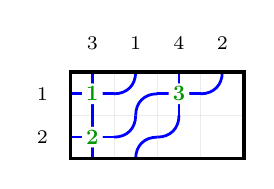
\begin{tikzpicture}[scale=0.55]
  \draw[lightgray, very thin, opacity=0.3] (0,2) -- (4,2);
  \draw[lightgray, very thin, opacity=0.3] (0,3) -- (4,3);
  \draw[lightgray, very thin, opacity=0.3] (0,4) -- (4,4);
  \draw[lightgray, very thin, opacity=0.3] (0,2) -- (0,4);
  \draw[lightgray, very thin, opacity=0.3] (1,2) -- (1,4);
  \draw[lightgray, very thin, opacity=0.3] (2,2) -- (2,4);
  \draw[lightgray, very thin, opacity=0.3] (3,2) -- (3,4);
  \draw[lightgray, very thin, opacity=0.3] (4,2) -- (4,4);
  \draw[blue, line width=1.0pt, line cap=round] (0,3.5) -- (1,3.5);
  \draw[blue, line width=1.0pt, line cap=round] (0.5,3) -- (0.5,4);
  \draw[blue, line width=1.0pt] (1,3.5) .. controls (1.3,3.5) and (1.5,3.7) .. (1.5,4);
  \draw[blue, line width=1.0pt] (1.5,3) .. controls (1.5,3.3) and (1.7,3.5) .. (2,3.5);
  \draw[blue, line width=1.0pt, line cap=round] (2,3.5) -- (3,3.5);
  \draw[blue, line width=1.0pt, line cap=round] (2.5,3) -- (2.5,4);
  \draw[blue, line width=1.0pt] (3,3.5) .. controls (3.3,3.5) and (3.5,3.7) .. (3.5,4);
  \draw[blue, line width=1.0pt, line cap=round] (0,2.5) -- (1,2.5);
  \draw[blue, line width=1.0pt, line cap=round] (0.5,2) -- (0.5,3);
  \draw[blue, line width=1.0pt] (1,2.5) .. controls (1.3,2.5) and (1.5,2.7) .. (1.5,3);
  \draw[blue, line width=1.0pt] (1.5,2) .. controls (1.5,2.3) and (1.7,2.5) .. (2,2.5);
  \draw[blue, line width=1.0pt] (2,2.5) .. controls (2.3,2.5) and (2.5,2.7) .. (2.5,3);
  \node[font=\Large\bfseries, text=green!60!black, fill=white, inner sep=0.5pt, circle, transform shape] at (0.5,3.5) {1};
  \node[font=\Large\bfseries, text=green!60!black, fill=white, inner sep=0.5pt, circle, transform shape] at (2.5,3.5) {3};
  \node[font=\Large\bfseries, text=green!60!black, fill=white, inner sep=0.5pt, circle, transform shape] at (0.5,2.5) {2};
  \node[font=\scriptsize, text=black, anchor=south] at (0.5,4.3) {3};
  \node[font=\scriptsize, text=black, anchor=south] at (1.5,4.3) {1};
  \node[font=\scriptsize, text=black, anchor=south] at (2.5,4.3) {4};
  \node[font=\scriptsize, text=black, anchor=south] at (3.5,4.3) {2};
  \node[font=\scriptsize, text=black, anchor=east] at (-0.3,3.5) {1};
  \node[font=\scriptsize, text=black, anchor=east] at (-0.3,2.5) {2};
  \draw[black, line width=1.2000000000000002pt] (0,2) rectangle (4,4);
\end{tikzpicture}}}
  \sqcupplus
  \vcenter{\hbox{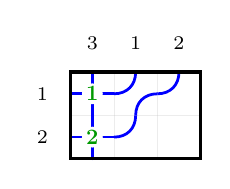
\begin{tikzpicture}[scale=0.55]
  \draw[lightgray, very thin, opacity=0.3] (0,1) -- (3,1);
  \draw[lightgray, very thin, opacity=0.3] (0,2) -- (3,2);
  \draw[lightgray, very thin, opacity=0.3] (0,3) -- (3,3);
  \draw[lightgray, very thin, opacity=0.3] (0,1) -- (0,3);
  \draw[lightgray, very thin, opacity=0.3] (1,1) -- (1,3);
  \draw[lightgray, very thin, opacity=0.3] (2,1) -- (2,3);
  \draw[lightgray, very thin, opacity=0.3] (3,1) -- (3,3);
  \draw[blue, line width=1.0pt, line cap=round] (0,2.5) -- (1,2.5);
  \draw[blue, line width=1.0pt, line cap=round] (0.5,2) -- (0.5,3);
  \draw[blue, line width=1.0pt] (1,2.5) .. controls (1.3,2.5) and (1.5,2.7) .. (1.5,3);
  \draw[blue, line width=1.0pt] (1.5,2) .. controls (1.5,2.3) and (1.7,2.5) .. (2,2.5);
  \draw[blue, line width=1.0pt] (2,2.5) .. controls (2.3,2.5) and (2.5,2.7) .. (2.5,3);
  \draw[blue, line width=1.0pt, line cap=round] (0,1.5) -- (1,1.5);
  \draw[blue, line width=1.0pt, line cap=round] (0.5,1) -- (0.5,2);
  \draw[blue, line width=1.0pt] (1,1.5) .. controls (1.3,1.5) and (1.5,1.7) .. (1.5,2);
  \node[font=\Large\bfseries, text=green!60!black, fill=white, inner sep=0.5pt, circle, transform shape] at (0.5,2.5) {1};
  \node[font=\Large\bfseries, text=green!60!black, fill=white, inner sep=0.5pt, circle, transform shape] at (0.5,1.5) {2};
  \node[font=\scriptsize, text=black, anchor=south] at (0.5,3.3) {3};
  \node[font=\scriptsize, text=black, anchor=south] at (1.5,3.3) {1};
  \node[font=\scriptsize, text=black, anchor=south] at (2.5,3.3) {2};
  \node[font=\scriptsize, text=black, anchor=east] at (-0.3,2.5) {1};
  \node[font=\scriptsize, text=black, anchor=east] at (-0.3,1.5) {2};
  \draw[black, line width=1.2000000000000002pt] (0,1) rectangle (3,3);
\end{tikzpicture}}}
  \\[1em]
  ={}& 
  \vcenter{\hbox{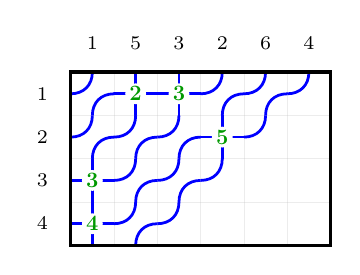
\begin{tikzpicture}[scale=0.55]
  \draw[lightgray, very thin, opacity=0.3] (0,2) -- (6,2);
  \draw[lightgray, very thin, opacity=0.3] (0,3) -- (6,3);
  \draw[lightgray, very thin, opacity=0.3] (0,4) -- (6,4);
  \draw[lightgray, very thin, opacity=0.3] (0,5) -- (6,5);
  \draw[lightgray, very thin, opacity=0.3] (0,6) -- (6,6);
  \draw[lightgray, very thin, opacity=0.3] (0,2) -- (0,6);
  \draw[lightgray, very thin, opacity=0.3] (1,2) -- (1,6);
  \draw[lightgray, very thin, opacity=0.3] (2,2) -- (2,6);
  \draw[lightgray, very thin, opacity=0.3] (3,2) -- (3,6);
  \draw[lightgray, very thin, opacity=0.3] (4,2) -- (4,6);
  \draw[lightgray, very thin, opacity=0.3] (5,2) -- (5,6);
  \draw[lightgray, very thin, opacity=0.3] (6,2) -- (6,6);
  \draw[blue, line width=1.0pt] (0,5.5) .. controls (0.3,5.5) and (0.5,5.7) .. (0.5,6);
  \draw[blue, line width=1.0pt] (0.5,5) .. controls (0.5,5.3) and (0.7,5.5) .. (1,5.5);
  \draw[blue, line width=1.0pt, line cap=round] (1,5.5) -- (2,5.5);
  \draw[blue, line width=1.0pt, line cap=round] (1.5,5) -- (1.5,6);
  \draw[blue, line width=1.0pt, line cap=round] (2,5.5) -- (3,5.5);
  \draw[blue, line width=1.0pt, line cap=round] (2.5,5) -- (2.5,6);
  \draw[blue, line width=1.0pt] (3,5.5) .. controls (3.3,5.5) and (3.5,5.7) .. (3.5,6);
  \draw[blue, line width=1.0pt] (3.5,5) .. controls (3.5,5.3) and (3.7,5.5) .. (4,5.5);
  \draw[blue, line width=1.0pt] (4,5.5) .. controls (4.3,5.5) and (4.5,5.7) .. (4.5,6);
  \draw[blue, line width=1.0pt] (4.5,5) .. controls (4.5,5.3) and (4.7,5.5) .. (5,5.5);
  \draw[blue, line width=1.0pt] (5,5.5) .. controls (5.3,5.5) and (5.5,5.7) .. (5.5,6);
  \draw[blue, line width=1.0pt] (0,4.5) .. controls (0.3,4.5) and (0.5,4.7) .. (0.5,5);
  \draw[blue, line width=1.0pt] (0.5,4) .. controls (0.5,4.3) and (0.7,4.5) .. (1,4.5);
  \draw[blue, line width=1.0pt] (1,4.5) .. controls (1.3,4.5) and (1.5,4.7) .. (1.5,5);
  \draw[blue, line width=1.0pt] (1.5,4) .. controls (1.5,4.3) and (1.7,4.5) .. (2,4.5);
  \draw[blue, line width=1.0pt] (2,4.5) .. controls (2.3,4.5) and (2.5,4.7) .. (2.5,5);
  \draw[blue, line width=1.0pt] (2.5,4) .. controls (2.5,4.3) and (2.7,4.5) .. (3,4.5);
  \draw[blue, line width=1.0pt, line cap=round] (3,4.5) -- (4,4.5);
  \draw[blue, line width=1.0pt, line cap=round] (3.5,4) -- (3.5,5);
  \draw[blue, line width=1.0pt] (4,4.5) .. controls (4.3,4.5) and (4.5,4.7) .. (4.5,5);
  \draw[blue, line width=1.0pt, line cap=round] (0,3.5) -- (1,3.5);
  \draw[blue, line width=1.0pt, line cap=round] (0.5,3) -- (0.5,4);
  \draw[blue, line width=1.0pt] (1,3.5) .. controls (1.3,3.5) and (1.5,3.7) .. (1.5,4);
  \draw[blue, line width=1.0pt] (1.5,3) .. controls (1.5,3.3) and (1.7,3.5) .. (2,3.5);
  \draw[blue, line width=1.0pt] (2,3.5) .. controls (2.3,3.5) and (2.5,3.7) .. (2.5,4);
  \draw[blue, line width=1.0pt] (2.5,3) .. controls (2.5,3.3) and (2.7,3.5) .. (3,3.5);
  \draw[blue, line width=1.0pt] (3,3.5) .. controls (3.3,3.5) and (3.5,3.7) .. (3.5,4);
  \draw[blue, line width=1.0pt, line cap=round] (0,2.5) -- (1,2.5);
  \draw[blue, line width=1.0pt, line cap=round] (0.5,2) -- (0.5,3);
  \draw[blue, line width=1.0pt] (1,2.5) .. controls (1.3,2.5) and (1.5,2.7) .. (1.5,3);
  \draw[blue, line width=1.0pt] (1.5,2) .. controls (1.5,2.3) and (1.7,2.5) .. (2,2.5);
  \draw[blue, line width=1.0pt] (2,2.5) .. controls (2.3,2.5) and (2.5,2.7) .. (2.5,3);
  \node[font=\Large\bfseries, text=green!60!black, fill=white, inner sep=0.5pt, circle, transform shape] at (3.5,4.5) {5};
  \node[font=\Large\bfseries, text=green!60!black, fill=white, inner sep=0.5pt, circle, transform shape] at (1.5,5.5) {2};
  \node[font=\Large\bfseries, text=green!60!black, fill=white, inner sep=0.5pt, circle, transform shape] at (0.5,2.5) {4};
  \node[font=\Large\bfseries, text=green!60!black, fill=white, inner sep=0.5pt, circle, transform shape] at (0.5,3.5) {3};
  \node[font=\Large\bfseries, text=green!60!black, fill=white, inner sep=0.5pt, circle, transform shape] at (2.5,5.5) {3};
  \node[font=\scriptsize, text=black, anchor=south] at (0.5,6.3) {1};
  \node[font=\scriptsize, text=black, anchor=south] at (1.5,6.3) {5};
  \node[font=\scriptsize, text=black, anchor=south] at (2.5,6.3) {3};
  \node[font=\scriptsize, text=black, anchor=south] at (3.5,6.3) {2};
  \node[font=\scriptsize, text=black, anchor=south] at (4.5,6.3) {6};
  \node[font=\scriptsize, text=black, anchor=south] at (5.5,6.3) {4};
  \node[font=\scriptsize, text=black, anchor=east] at (-0.3,5.5) {1};
  \node[font=\scriptsize, text=black, anchor=east] at (-0.3,4.5) {2};
  \node[font=\scriptsize, text=black, anchor=east] at (-0.3,3.5) {3};
  \node[font=\scriptsize, text=black, anchor=east] at (-0.3,2.5) {4};
  \draw[black, line width=1.2000000000000002pt] (0,2) rectangle (6,6);
\end{tikzpicture}}}
  +
  \vcenter{\hbox{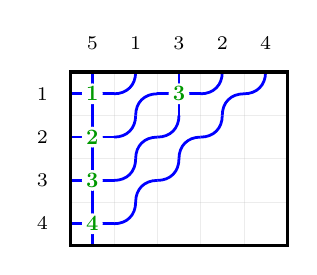
\begin{tikzpicture}[scale=0.55]
  \draw[lightgray, very thin, opacity=0.3] (0,1) -- (5,1);
  \draw[lightgray, very thin, opacity=0.3] (0,2) -- (5,2);
  \draw[lightgray, very thin, opacity=0.3] (0,3) -- (5,3);
  \draw[lightgray, very thin, opacity=0.3] (0,4) -- (5,4);
  \draw[lightgray, very thin, opacity=0.3] (0,5) -- (5,5);
  \draw[lightgray, very thin, opacity=0.3] (0,1) -- (0,5);
  \draw[lightgray, very thin, opacity=0.3] (1,1) -- (1,5);
  \draw[lightgray, very thin, opacity=0.3] (2,1) -- (2,5);
  \draw[lightgray, very thin, opacity=0.3] (3,1) -- (3,5);
  \draw[lightgray, very thin, opacity=0.3] (4,1) -- (4,5);
  \draw[lightgray, very thin, opacity=0.3] (5,1) -- (5,5);
  \draw[blue, line width=1.0pt, line cap=round] (0,4.5) -- (1,4.5);
  \draw[blue, line width=1.0pt, line cap=round] (0.5,4) -- (0.5,5);
  \draw[blue, line width=1.0pt] (1,4.5) .. controls (1.3,4.5) and (1.5,4.7) .. (1.5,5);
  \draw[blue, line width=1.0pt] (1.5,4) .. controls (1.5,4.3) and (1.7,4.5) .. (2,4.5);
  \draw[blue, line width=1.0pt, line cap=round] (2,4.5) -- (3,4.5);
  \draw[blue, line width=1.0pt, line cap=round] (2.5,4) -- (2.5,5);
  \draw[blue, line width=1.0pt] (3,4.5) .. controls (3.3,4.5) and (3.5,4.7) .. (3.5,5);
  \draw[blue, line width=1.0pt] (3.5,4) .. controls (3.5,4.3) and (3.7,4.5) .. (4,4.5);
  \draw[blue, line width=1.0pt] (4,4.5) .. controls (4.3,4.5) and (4.5,4.7) .. (4.5,5);
  \draw[blue, line width=1.0pt, line cap=round] (0,3.5) -- (1,3.5);
  \draw[blue, line width=1.0pt, line cap=round] (0.5,3) -- (0.5,4);
  \draw[blue, line width=1.0pt] (1,3.5) .. controls (1.3,3.5) and (1.5,3.7) .. (1.5,4);
  \draw[blue, line width=1.0pt] (1.5,3) .. controls (1.5,3.3) and (1.7,3.5) .. (2,3.5);
  \draw[blue, line width=1.0pt] (2,3.5) .. controls (2.3,3.5) and (2.5,3.7) .. (2.5,4);
  \draw[blue, line width=1.0pt] (2.5,3) .. controls (2.5,3.3) and (2.7,3.5) .. (3,3.5);
  \draw[blue, line width=1.0pt] (3,3.5) .. controls (3.3,3.5) and (3.5,3.7) .. (3.5,4);
  \draw[blue, line width=1.0pt, line cap=round] (0,2.5) -- (1,2.5);
  \draw[blue, line width=1.0pt, line cap=round] (0.5,2) -- (0.5,3);
  \draw[blue, line width=1.0pt] (1,2.5) .. controls (1.3,2.5) and (1.5,2.7) .. (1.5,3);
  \draw[blue, line width=1.0pt] (1.5,2) .. controls (1.5,2.3) and (1.7,2.5) .. (2,2.5);
  \draw[blue, line width=1.0pt] (2,2.5) .. controls (2.3,2.5) and (2.5,2.7) .. (2.5,3);
  \draw[blue, line width=1.0pt, line cap=round] (0,1.5) -- (1,1.5);
  \draw[blue, line width=1.0pt, line cap=round] (0.5,1) -- (0.5,2);
  \draw[blue, line width=1.0pt] (1,1.5) .. controls (1.3,1.5) and (1.5,1.7) .. (1.5,2);
  \node[font=\Large\bfseries, text=green!60!black, fill=white, inner sep=0.5pt, circle, transform shape] at (0.5,3.5) {2};
  \node[font=\Large\bfseries, text=green!60!black, fill=white, inner sep=0.5pt, circle, transform shape] at (0.5,1.5) {4};
  \node[font=\Large\bfseries, text=green!60!black, fill=white, inner sep=0.5pt, circle, transform shape] at (0.5,2.5) {3};
  \node[font=\Large\bfseries, text=green!60!black, fill=white, inner sep=0.5pt, circle, transform shape] at (0.5,4.5) {1};
  \node[font=\Large\bfseries, text=green!60!black, fill=white, inner sep=0.5pt, circle, transform shape] at (2.5,4.5) {3};
  \node[font=\scriptsize, text=black, anchor=south] at (0.5,5.3) {5};
  \node[font=\scriptsize, text=black, anchor=south] at (1.5,5.3) {1};
  \node[font=\scriptsize, text=black, anchor=south] at (2.5,5.3) {3};
  \node[font=\scriptsize, text=black, anchor=south] at (3.5,5.3) {2};
  \node[font=\scriptsize, text=black, anchor=south] at (4.5,5.3) {4};
  \node[font=\scriptsize, text=black, anchor=east] at (-0.3,4.5) {1};
  \node[font=\scriptsize, text=black, anchor=east] at (-0.3,3.5) {2};
  \node[font=\scriptsize, text=black, anchor=east] at (-0.3,2.5) {3};
  \node[font=\scriptsize, text=black, anchor=east] at (-0.3,1.5) {4};
  \draw[black, line width=1.2000000000000002pt] (0,1) rectangle (5,5);
\end{tikzpicture}}}
  +
  \vcenter{\hbox{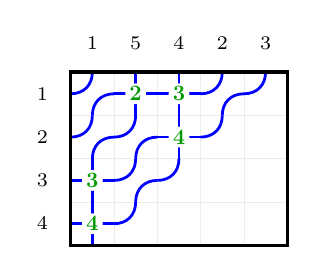
\begin{tikzpicture}[scale=0.55]
  \draw[lightgray, very thin, opacity=0.3] (0,1) -- (5,1);
  \draw[lightgray, very thin, opacity=0.3] (0,2) -- (5,2);
  \draw[lightgray, very thin, opacity=0.3] (0,3) -- (5,3);
  \draw[lightgray, very thin, opacity=0.3] (0,4) -- (5,4);
  \draw[lightgray, very thin, opacity=0.3] (0,5) -- (5,5);
  \draw[lightgray, very thin, opacity=0.3] (0,1) -- (0,5);
  \draw[lightgray, very thin, opacity=0.3] (1,1) -- (1,5);
  \draw[lightgray, very thin, opacity=0.3] (2,1) -- (2,5);
  \draw[lightgray, very thin, opacity=0.3] (3,1) -- (3,5);
  \draw[lightgray, very thin, opacity=0.3] (4,1) -- (4,5);
  \draw[lightgray, very thin, opacity=0.3] (5,1) -- (5,5);
  \draw[blue, line width=1.0pt] (0,4.5) .. controls (0.3,4.5) and (0.5,4.7) .. (0.5,5);
  \draw[blue, line width=1.0pt] (0.5,4) .. controls (0.5,4.3) and (0.7,4.5) .. (1,4.5);
  \draw[blue, line width=1.0pt, line cap=round] (1,4.5) -- (2,4.5);
  \draw[blue, line width=1.0pt, line cap=round] (1.5,4) -- (1.5,5);
  \draw[blue, line width=1.0pt, line cap=round] (2,4.5) -- (3,4.5);
  \draw[blue, line width=1.0pt, line cap=round] (2.5,4) -- (2.5,5);
  \draw[blue, line width=1.0pt] (3,4.5) .. controls (3.3,4.5) and (3.5,4.7) .. (3.5,5);
  \draw[blue, line width=1.0pt] (3.5,4) .. controls (3.5,4.3) and (3.7,4.5) .. (4,4.5);
  \draw[blue, line width=1.0pt] (4,4.5) .. controls (4.3,4.5) and (4.5,4.7) .. (4.5,5);
  \draw[blue, line width=1.0pt] (0,3.5) .. controls (0.3,3.5) and (0.5,3.7) .. (0.5,4);
  \draw[blue, line width=1.0pt] (0.5,3) .. controls (0.5,3.3) and (0.7,3.5) .. (1,3.5);
  \draw[blue, line width=1.0pt] (1,3.5) .. controls (1.3,3.5) and (1.5,3.7) .. (1.5,4);
  \draw[blue, line width=1.0pt] (1.5,3) .. controls (1.5,3.3) and (1.7,3.5) .. (2,3.5);
  \draw[blue, line width=1.0pt, line cap=round] (2,3.5) -- (3,3.5);
  \draw[blue, line width=1.0pt, line cap=round] (2.5,3) -- (2.5,4);
  \draw[blue, line width=1.0pt] (3,3.5) .. controls (3.3,3.5) and (3.5,3.7) .. (3.5,4);
  \draw[blue, line width=1.0pt, line cap=round] (0,2.5) -- (1,2.5);
  \draw[blue, line width=1.0pt, line cap=round] (0.5,2) -- (0.5,3);
  \draw[blue, line width=1.0pt] (1,2.5) .. controls (1.3,2.5) and (1.5,2.7) .. (1.5,3);
  \draw[blue, line width=1.0pt] (1.5,2) .. controls (1.5,2.3) and (1.7,2.5) .. (2,2.5);
  \draw[blue, line width=1.0pt] (2,2.5) .. controls (2.3,2.5) and (2.5,2.7) .. (2.5,3);
  \draw[blue, line width=1.0pt, line cap=round] (0,1.5) -- (1,1.5);
  \draw[blue, line width=1.0pt, line cap=round] (0.5,1) -- (0.5,2);
  \draw[blue, line width=1.0pt] (1,1.5) .. controls (1.3,1.5) and (1.5,1.7) .. (1.5,2);
  \node[font=\Large\bfseries, text=green!60!black, fill=white, inner sep=0.5pt, circle, transform shape] at (1.5,4.5) {2};
  \node[font=\Large\bfseries, text=green!60!black, fill=white, inner sep=0.5pt, circle, transform shape] at (0.5,1.5) {4};
  \node[font=\Large\bfseries, text=green!60!black, fill=white, inner sep=0.5pt, circle, transform shape] at (0.5,2.5) {3};
  \node[font=\Large\bfseries, text=green!60!black, fill=white, inner sep=0.5pt, circle, transform shape] at (2.5,3.5) {4};
  \node[font=\Large\bfseries, text=green!60!black, fill=white, inner sep=0.5pt, circle, transform shape] at (2.5,4.5) {3};
  \node[font=\scriptsize, text=black, anchor=south] at (0.5,5.3) {1};
  \node[font=\scriptsize, text=black, anchor=south] at (1.5,5.3) {5};
  \node[font=\scriptsize, text=black, anchor=south] at (2.5,5.3) {4};
  \node[font=\scriptsize, text=black, anchor=south] at (3.5,5.3) {2};
  \node[font=\scriptsize, text=black, anchor=south] at (4.5,5.3) {3};
  \node[font=\scriptsize, text=black, anchor=east] at (-0.3,4.5) {1};
  \node[font=\scriptsize, text=black, anchor=east] at (-0.3,3.5) {2};
  \node[font=\scriptsize, text=black, anchor=east] at (-0.3,2.5) {3};
  \node[font=\scriptsize, text=black, anchor=east] at (-0.3,1.5) {4};
  \draw[black, line width=1.2000000000000002pt] (0,1) rectangle (5,5);
\end{tikzpicture}}}
  \\[1em]
  + & 
  \vcenter{\hbox{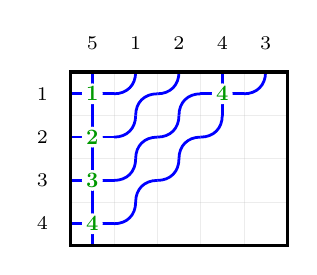
\begin{tikzpicture}[scale=0.55]
  \draw[lightgray, very thin, opacity=0.3] (0,1) -- (5,1);
  \draw[lightgray, very thin, opacity=0.3] (0,2) -- (5,2);
  \draw[lightgray, very thin, opacity=0.3] (0,3) -- (5,3);
  \draw[lightgray, very thin, opacity=0.3] (0,4) -- (5,4);
  \draw[lightgray, very thin, opacity=0.3] (0,5) -- (5,5);
  \draw[lightgray, very thin, opacity=0.3] (0,1) -- (0,5);
  \draw[lightgray, very thin, opacity=0.3] (1,1) -- (1,5);
  \draw[lightgray, very thin, opacity=0.3] (2,1) -- (2,5);
  \draw[lightgray, very thin, opacity=0.3] (3,1) -- (3,5);
  \draw[lightgray, very thin, opacity=0.3] (4,1) -- (4,5);
  \draw[lightgray, very thin, opacity=0.3] (5,1) -- (5,5);
  \draw[blue, line width=1.0pt, line cap=round] (0,4.5) -- (1,4.5);
  \draw[blue, line width=1.0pt, line cap=round] (0.5,4) -- (0.5,5);
  \draw[blue, line width=1.0pt] (1,4.5) .. controls (1.3,4.5) and (1.5,4.7) .. (1.5,5);
  \draw[blue, line width=1.0pt] (1.5,4) .. controls (1.5,4.3) and (1.7,4.5) .. (2,4.5);
  \draw[blue, line width=1.0pt] (2,4.5) .. controls (2.3,4.5) and (2.5,4.7) .. (2.5,5);
  \draw[blue, line width=1.0pt] (2.5,4) .. controls (2.5,4.3) and (2.7,4.5) .. (3,4.5);
  \draw[blue, line width=1.0pt, line cap=round] (3,4.5) -- (4,4.5);
  \draw[blue, line width=1.0pt, line cap=round] (3.5,4) -- (3.5,5);
  \draw[blue, line width=1.0pt] (4,4.5) .. controls (4.3,4.5) and (4.5,4.7) .. (4.5,5);
  \draw[blue, line width=1.0pt, line cap=round] (0,3.5) -- (1,3.5);
  \draw[blue, line width=1.0pt, line cap=round] (0.5,3) -- (0.5,4);
  \draw[blue, line width=1.0pt] (1,3.5) .. controls (1.3,3.5) and (1.5,3.7) .. (1.5,4);
  \draw[blue, line width=1.0pt] (1.5,3) .. controls (1.5,3.3) and (1.7,3.5) .. (2,3.5);
  \draw[blue, line width=1.0pt] (2,3.5) .. controls (2.3,3.5) and (2.5,3.7) .. (2.5,4);
  \draw[blue, line width=1.0pt] (2.5,3) .. controls (2.5,3.3) and (2.7,3.5) .. (3,3.5);
  \draw[blue, line width=1.0pt] (3,3.5) .. controls (3.3,3.5) and (3.5,3.7) .. (3.5,4);
  \draw[blue, line width=1.0pt, line cap=round] (0,2.5) -- (1,2.5);
  \draw[blue, line width=1.0pt, line cap=round] (0.5,2) -- (0.5,3);
  \draw[blue, line width=1.0pt] (1,2.5) .. controls (1.3,2.5) and (1.5,2.7) .. (1.5,3);
  \draw[blue, line width=1.0pt] (1.5,2) .. controls (1.5,2.3) and (1.7,2.5) .. (2,2.5);
  \draw[blue, line width=1.0pt] (2,2.5) .. controls (2.3,2.5) and (2.5,2.7) .. (2.5,3);
  \draw[blue, line width=1.0pt, line cap=round] (0,1.5) -- (1,1.5);
  \draw[blue, line width=1.0pt, line cap=round] (0.5,1) -- (0.5,2);
  \draw[blue, line width=1.0pt] (1,1.5) .. controls (1.3,1.5) and (1.5,1.7) .. (1.5,2);
  \node[font=\Large\bfseries, text=green!60!black, fill=white, inner sep=0.5pt, circle, transform shape] at (0.5,3.5) {2};
  \node[font=\Large\bfseries, text=green!60!black, fill=white, inner sep=0.5pt, circle, transform shape] at (0.5,2.5) {3};
  \node[font=\Large\bfseries, text=green!60!black, fill=white, inner sep=0.5pt, circle, transform shape] at (0.5,4.5) {1};
  \node[font=\Large\bfseries, text=green!60!black, fill=white, inner sep=0.5pt, circle, transform shape] at (3.5,4.5) {4};
  \node[font=\Large\bfseries, text=green!60!black, fill=white, inner sep=0.5pt, circle, transform shape] at (0.5,1.5) {4};
  \node[font=\scriptsize, text=black, anchor=south] at (0.5,5.3) {5};
  \node[font=\scriptsize, text=black, anchor=south] at (1.5,5.3) {1};
  \node[font=\scriptsize, text=black, anchor=south] at (2.5,5.3) {2};
  \node[font=\scriptsize, text=black, anchor=south] at (3.5,5.3) {4};
  \node[font=\scriptsize, text=black, anchor=south] at (4.5,5.3) {3};
  \node[font=\scriptsize, text=black, anchor=east] at (-0.3,4.5) {1};
  \node[font=\scriptsize, text=black, anchor=east] at (-0.3,3.5) {2};
  \node[font=\scriptsize, text=black, anchor=east] at (-0.3,2.5) {3};
  \node[font=\scriptsize, text=black, anchor=east] at (-0.3,1.5) {4};
  \draw[black, line width=1.2000000000000002pt] (0,1) rectangle (5,5);
\end{tikzpicture}}}
  +
  \vcenter{\hbox{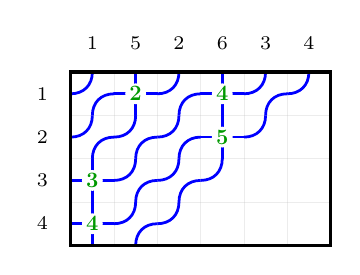
\begin{tikzpicture}[scale=0.55]
  \draw[lightgray, very thin, opacity=0.3] (0,2) -- (6,2);
  \draw[lightgray, very thin, opacity=0.3] (0,3) -- (6,3);
  \draw[lightgray, very thin, opacity=0.3] (0,4) -- (6,4);
  \draw[lightgray, very thin, opacity=0.3] (0,5) -- (6,5);
  \draw[lightgray, very thin, opacity=0.3] (0,6) -- (6,6);
  \draw[lightgray, very thin, opacity=0.3] (0,2) -- (0,6);
  \draw[lightgray, very thin, opacity=0.3] (1,2) -- (1,6);
  \draw[lightgray, very thin, opacity=0.3] (2,2) -- (2,6);
  \draw[lightgray, very thin, opacity=0.3] (3,2) -- (3,6);
  \draw[lightgray, very thin, opacity=0.3] (4,2) -- (4,6);
  \draw[lightgray, very thin, opacity=0.3] (5,2) -- (5,6);
  \draw[lightgray, very thin, opacity=0.3] (6,2) -- (6,6);
  \draw[blue, line width=1.0pt] (0,5.5) .. controls (0.3,5.5) and (0.5,5.7) .. (0.5,6);
  \draw[blue, line width=1.0pt] (0.5,5) .. controls (0.5,5.3) and (0.7,5.5) .. (1,5.5);
  \draw[blue, line width=1.0pt, line cap=round] (1,5.5) -- (2,5.5);
  \draw[blue, line width=1.0pt, line cap=round] (1.5,5) -- (1.5,6);
  \draw[blue, line width=1.0pt] (2,5.5) .. controls (2.3,5.5) and (2.5,5.7) .. (2.5,6);
  \draw[blue, line width=1.0pt] (2.5,5) .. controls (2.5,5.3) and (2.7,5.5) .. (3,5.5);
  \draw[blue, line width=1.0pt, line cap=round] (3,5.5) -- (4,5.5);
  \draw[blue, line width=1.0pt, line cap=round] (3.5,5) -- (3.5,6);
  \draw[blue, line width=1.0pt] (4,5.5) .. controls (4.3,5.5) and (4.5,5.7) .. (4.5,6);
  \draw[blue, line width=1.0pt] (4.5,5) .. controls (4.5,5.3) and (4.7,5.5) .. (5,5.5);
  \draw[blue, line width=1.0pt] (5,5.5) .. controls (5.3,5.5) and (5.5,5.7) .. (5.5,6);
  \draw[blue, line width=1.0pt] (0,4.5) .. controls (0.3,4.5) and (0.5,4.7) .. (0.5,5);
  \draw[blue, line width=1.0pt] (0.5,4) .. controls (0.5,4.3) and (0.7,4.5) .. (1,4.5);
  \draw[blue, line width=1.0pt] (1,4.5) .. controls (1.3,4.5) and (1.5,4.7) .. (1.5,5);
  \draw[blue, line width=1.0pt] (1.5,4) .. controls (1.5,4.3) and (1.7,4.5) .. (2,4.5);
  \draw[blue, line width=1.0pt] (2,4.5) .. controls (2.3,4.5) and (2.5,4.7) .. (2.5,5);
  \draw[blue, line width=1.0pt] (2.5,4) .. controls (2.5,4.3) and (2.7,4.5) .. (3,4.5);
  \draw[blue, line width=1.0pt, line cap=round] (3,4.5) -- (4,4.5);
  \draw[blue, line width=1.0pt, line cap=round] (3.5,4) -- (3.5,5);
  \draw[blue, line width=1.0pt] (4,4.5) .. controls (4.3,4.5) and (4.5,4.7) .. (4.5,5);
  \draw[blue, line width=1.0pt, line cap=round] (0,3.5) -- (1,3.5);
  \draw[blue, line width=1.0pt, line cap=round] (0.5,3) -- (0.5,4);
  \draw[blue, line width=1.0pt] (1,3.5) .. controls (1.3,3.5) and (1.5,3.7) .. (1.5,4);
  \draw[blue, line width=1.0pt] (1.5,3) .. controls (1.5,3.3) and (1.7,3.5) .. (2,3.5);
  \draw[blue, line width=1.0pt] (2,3.5) .. controls (2.3,3.5) and (2.5,3.7) .. (2.5,4);
  \draw[blue, line width=1.0pt] (2.5,3) .. controls (2.5,3.3) and (2.7,3.5) .. (3,3.5);
  \draw[blue, line width=1.0pt] (3,3.5) .. controls (3.3,3.5) and (3.5,3.7) .. (3.5,4);
  \draw[blue, line width=1.0pt, line cap=round] (0,2.5) -- (1,2.5);
  \draw[blue, line width=1.0pt, line cap=round] (0.5,2) -- (0.5,3);
  \draw[blue, line width=1.0pt] (1,2.5) .. controls (1.3,2.5) and (1.5,2.7) .. (1.5,3);
  \draw[blue, line width=1.0pt] (1.5,2) .. controls (1.5,2.3) and (1.7,2.5) .. (2,2.5);
  \draw[blue, line width=1.0pt] (2,2.5) .. controls (2.3,2.5) and (2.5,2.7) .. (2.5,3);
  \node[font=\Large\bfseries, text=green!60!black, fill=white, inner sep=0.5pt, circle, transform shape] at (3.5,4.5) {5};
  \node[font=\Large\bfseries, text=green!60!black, fill=white, inner sep=0.5pt, circle, transform shape] at (1.5,5.5) {2};
  \node[font=\Large\bfseries, text=green!60!black, fill=white, inner sep=0.5pt, circle, transform shape] at (0.5,3.5) {3};
  \node[font=\Large\bfseries, text=green!60!black, fill=white, inner sep=0.5pt, circle, transform shape] at (3.5,5.5) {4};
  \node[font=\Large\bfseries, text=green!60!black, fill=white, inner sep=0.5pt, circle, transform shape] at (0.5,2.5) {4};
  \node[font=\scriptsize, text=black, anchor=south] at (0.5,6.3) {1};
  \node[font=\scriptsize, text=black, anchor=south] at (1.5,6.3) {5};
  \node[font=\scriptsize, text=black, anchor=south] at (2.5,6.3) {2};
  \node[font=\scriptsize, text=black, anchor=south] at (3.5,6.3) {6};
  \node[font=\scriptsize, text=black, anchor=south] at (4.5,6.3) {3};
  \node[font=\scriptsize, text=black, anchor=south] at (5.5,6.3) {4};
  \node[font=\scriptsize, text=black, anchor=east] at (-0.3,5.5) {1};
  \node[font=\scriptsize, text=black, anchor=east] at (-0.3,4.5) {2};
  \node[font=\scriptsize, text=black, anchor=east] at (-0.3,3.5) {3};
  \node[font=\scriptsize, text=black, anchor=east] at (-0.3,2.5) {4};
  \draw[black, line width=1.2000000000000002pt] (0,2) rectangle (6,6);
\end{tikzpicture}}}
  +
  \vcenter{\hbox{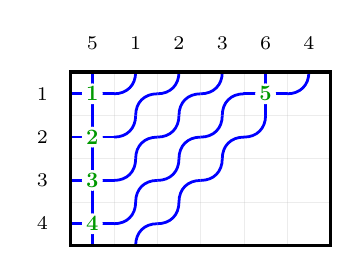
\begin{tikzpicture}[scale=0.55]
  \draw[lightgray, very thin, opacity=0.3] (0,2) -- (6,2);
  \draw[lightgray, very thin, opacity=0.3] (0,3) -- (6,3);
  \draw[lightgray, very thin, opacity=0.3] (0,4) -- (6,4);
  \draw[lightgray, very thin, opacity=0.3] (0,5) -- (6,5);
  \draw[lightgray, very thin, opacity=0.3] (0,6) -- (6,6);
  \draw[lightgray, very thin, opacity=0.3] (0,2) -- (0,6);
  \draw[lightgray, very thin, opacity=0.3] (1,2) -- (1,6);
  \draw[lightgray, very thin, opacity=0.3] (2,2) -- (2,6);
  \draw[lightgray, very thin, opacity=0.3] (3,2) -- (3,6);
  \draw[lightgray, very thin, opacity=0.3] (4,2) -- (4,6);
  \draw[lightgray, very thin, opacity=0.3] (5,2) -- (5,6);
  \draw[lightgray, very thin, opacity=0.3] (6,2) -- (6,6);
  \draw[blue, line width=1.0pt, line cap=round] (0,5.5) -- (1,5.5);
  \draw[blue, line width=1.0pt, line cap=round] (0.5,5) -- (0.5,6);
  \draw[blue, line width=1.0pt] (1,5.5) .. controls (1.3,5.5) and (1.5,5.7) .. (1.5,6);
  \draw[blue, line width=1.0pt] (1.5,5) .. controls (1.5,5.3) and (1.7,5.5) .. (2,5.5);
  \draw[blue, line width=1.0pt] (2,5.5) .. controls (2.3,5.5) and (2.5,5.7) .. (2.5,6);
  \draw[blue, line width=1.0pt] (2.5,5) .. controls (2.5,5.3) and (2.7,5.5) .. (3,5.5);
  \draw[blue, line width=1.0pt] (3,5.5) .. controls (3.3,5.5) and (3.5,5.7) .. (3.5,6);
  \draw[blue, line width=1.0pt] (3.5,5) .. controls (3.5,5.3) and (3.7,5.5) .. (4,5.5);
  \draw[blue, line width=1.0pt, line cap=round] (4,5.5) -- (5,5.5);
  \draw[blue, line width=1.0pt, line cap=round] (4.5,5) -- (4.5,6);
  \draw[blue, line width=1.0pt] (5,5.5) .. controls (5.3,5.5) and (5.5,5.7) .. (5.5,6);
  \draw[blue, line width=1.0pt, line cap=round] (0,4.5) -- (1,4.5);
  \draw[blue, line width=1.0pt, line cap=round] (0.5,4) -- (0.5,5);
  \draw[blue, line width=1.0pt] (1,4.5) .. controls (1.3,4.5) and (1.5,4.7) .. (1.5,5);
  \draw[blue, line width=1.0pt] (1.5,4) .. controls (1.5,4.3) and (1.7,4.5) .. (2,4.5);
  \draw[blue, line width=1.0pt] (2,4.5) .. controls (2.3,4.5) and (2.5,4.7) .. (2.5,5);
  \draw[blue, line width=1.0pt] (2.5,4) .. controls (2.5,4.3) and (2.7,4.5) .. (3,4.5);
  \draw[blue, line width=1.0pt] (3,4.5) .. controls (3.3,4.5) and (3.5,4.7) .. (3.5,5);
  \draw[blue, line width=1.0pt] (3.5,4) .. controls (3.5,4.3) and (3.7,4.5) .. (4,4.5);
  \draw[blue, line width=1.0pt] (4,4.5) .. controls (4.3,4.5) and (4.5,4.7) .. (4.5,5);
  \draw[blue, line width=1.0pt, line cap=round] (0,3.5) -- (1,3.5);
  \draw[blue, line width=1.0pt, line cap=round] (0.5,3) -- (0.5,4);
  \draw[blue, line width=1.0pt] (1,3.5) .. controls (1.3,3.5) and (1.5,3.7) .. (1.5,4);
  \draw[blue, line width=1.0pt] (1.5,3) .. controls (1.5,3.3) and (1.7,3.5) .. (2,3.5);
  \draw[blue, line width=1.0pt] (2,3.5) .. controls (2.3,3.5) and (2.5,3.7) .. (2.5,4);
  \draw[blue, line width=1.0pt] (2.5,3) .. controls (2.5,3.3) and (2.7,3.5) .. (3,3.5);
  \draw[blue, line width=1.0pt] (3,3.5) .. controls (3.3,3.5) and (3.5,3.7) .. (3.5,4);
  \draw[blue, line width=1.0pt, line cap=round] (0,2.5) -- (1,2.5);
  \draw[blue, line width=1.0pt, line cap=round] (0.5,2) -- (0.5,3);
  \draw[blue, line width=1.0pt] (1,2.5) .. controls (1.3,2.5) and (1.5,2.7) .. (1.5,3);
  \draw[blue, line width=1.0pt] (1.5,2) .. controls (1.5,2.3) and (1.7,2.5) .. (2,2.5);
  \draw[blue, line width=1.0pt] (2,2.5) .. controls (2.3,2.5) and (2.5,2.7) .. (2.5,3);
  \node[font=\Large\bfseries, text=green!60!black, fill=white, inner sep=0.5pt, circle, transform shape] at (0.5,4.5) {2};
  \node[font=\Large\bfseries, text=green!60!black, fill=white, inner sep=0.5pt, circle, transform shape] at (4.5,5.5) {5};
  \node[font=\Large\bfseries, text=green!60!black, fill=white, inner sep=0.5pt, circle, transform shape] at (0.5,3.5) {3};
  \node[font=\Large\bfseries, text=green!60!black, fill=white, inner sep=0.5pt, circle, transform shape] at (0.5,5.5) {1};
  \node[font=\Large\bfseries, text=green!60!black, fill=white, inner sep=0.5pt, circle, transform shape] at (0.5,2.5) {4};
  \node[font=\scriptsize, text=black, anchor=south] at (0.5,6.3) {5};
  \node[font=\scriptsize, text=black, anchor=south] at (1.5,6.3) {1};
  \node[font=\scriptsize, text=black, anchor=south] at (2.5,6.3) {2};
  \node[font=\scriptsize, text=black, anchor=south] at (3.5,6.3) {3};
  \node[font=\scriptsize, text=black, anchor=south] at (4.5,6.3) {6};
  \node[font=\scriptsize, text=black, anchor=south] at (5.5,6.3) {4};
  \node[font=\scriptsize, text=black, anchor=east] at (-0.3,5.5) {1};
  \node[font=\scriptsize, text=black, anchor=east] at (-0.3,4.5) {2};
  \node[font=\scriptsize, text=black, anchor=east] at (-0.3,3.5) {3};
  \node[font=\scriptsize, text=black, anchor=east] at (-0.3,2.5) {4};
  \draw[black, line width=1.2000000000000002pt] (0,2) rectangle (6,6);
\end{tikzpicture}}}
  \\[1em]
  + & 
  \vcenter{\hbox{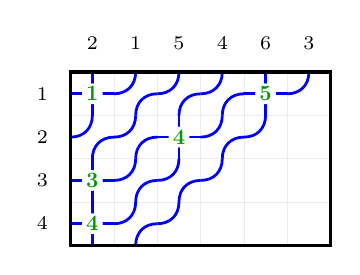
\begin{tikzpicture}[scale=0.55]
  \draw[lightgray, very thin, opacity=0.3] (0,2) -- (6,2);
  \draw[lightgray, very thin, opacity=0.3] (0,3) -- (6,3);
  \draw[lightgray, very thin, opacity=0.3] (0,4) -- (6,4);
  \draw[lightgray, very thin, opacity=0.3] (0,5) -- (6,5);
  \draw[lightgray, very thin, opacity=0.3] (0,6) -- (6,6);
  \draw[lightgray, very thin, opacity=0.3] (0,2) -- (0,6);
  \draw[lightgray, very thin, opacity=0.3] (1,2) -- (1,6);
  \draw[lightgray, very thin, opacity=0.3] (2,2) -- (2,6);
  \draw[lightgray, very thin, opacity=0.3] (3,2) -- (3,6);
  \draw[lightgray, very thin, opacity=0.3] (4,2) -- (4,6);
  \draw[lightgray, very thin, opacity=0.3] (5,2) -- (5,6);
  \draw[lightgray, very thin, opacity=0.3] (6,2) -- (6,6);
  \draw[blue, line width=1.0pt, line cap=round] (0,5.5) -- (1,5.5);
  \draw[blue, line width=1.0pt, line cap=round] (0.5,5) -- (0.5,6);
  \draw[blue, line width=1.0pt] (1,5.5) .. controls (1.3,5.5) and (1.5,5.7) .. (1.5,6);
  \draw[blue, line width=1.0pt] (1.5,5) .. controls (1.5,5.3) and (1.7,5.5) .. (2,5.5);
  \draw[blue, line width=1.0pt] (2,5.5) .. controls (2.3,5.5) and (2.5,5.7) .. (2.5,6);
  \draw[blue, line width=1.0pt] (2.5,5) .. controls (2.5,5.3) and (2.7,5.5) .. (3,5.5);
  \draw[blue, line width=1.0pt] (3,5.5) .. controls (3.3,5.5) and (3.5,5.7) .. (3.5,6);
  \draw[blue, line width=1.0pt] (3.5,5) .. controls (3.5,5.3) and (3.7,5.5) .. (4,5.5);
  \draw[blue, line width=1.0pt, line cap=round] (4,5.5) -- (5,5.5);
  \draw[blue, line width=1.0pt, line cap=round] (4.5,5) -- (4.5,6);
  \draw[blue, line width=1.0pt] (5,5.5) .. controls (5.3,5.5) and (5.5,5.7) .. (5.5,6);
  \draw[blue, line width=1.0pt] (0,4.5) .. controls (0.3,4.5) and (0.5,4.7) .. (0.5,5);
  \draw[blue, line width=1.0pt] (0.5,4) .. controls (0.5,4.3) and (0.7,4.5) .. (1,4.5);
  \draw[blue, line width=1.0pt] (1,4.5) .. controls (1.3,4.5) and (1.5,4.7) .. (1.5,5);
  \draw[blue, line width=1.0pt] (1.5,4) .. controls (1.5,4.3) and (1.7,4.5) .. (2,4.5);
  \draw[blue, line width=1.0pt, line cap=round] (2,4.5) -- (3,4.5);
  \draw[blue, line width=1.0pt, line cap=round] (2.5,4) -- (2.5,5);
  \draw[blue, line width=1.0pt] (3,4.5) .. controls (3.3,4.5) and (3.5,4.7) .. (3.5,5);
  \draw[blue, line width=1.0pt] (3.5,4) .. controls (3.5,4.3) and (3.7,4.5) .. (4,4.5);
  \draw[blue, line width=1.0pt] (4,4.5) .. controls (4.3,4.5) and (4.5,4.7) .. (4.5,5);
  \draw[blue, line width=1.0pt, line cap=round] (0,3.5) -- (1,3.5);
  \draw[blue, line width=1.0pt, line cap=round] (0.5,3) -- (0.5,4);
  \draw[blue, line width=1.0pt] (1,3.5) .. controls (1.3,3.5) and (1.5,3.7) .. (1.5,4);
  \draw[blue, line width=1.0pt] (1.5,3) .. controls (1.5,3.3) and (1.7,3.5) .. (2,3.5);
  \draw[blue, line width=1.0pt] (2,3.5) .. controls (2.3,3.5) and (2.5,3.7) .. (2.5,4);
  \draw[blue, line width=1.0pt] (2.5,3) .. controls (2.5,3.3) and (2.7,3.5) .. (3,3.5);
  \draw[blue, line width=1.0pt] (3,3.5) .. controls (3.3,3.5) and (3.5,3.7) .. (3.5,4);
  \draw[blue, line width=1.0pt, line cap=round] (0,2.5) -- (1,2.5);
  \draw[blue, line width=1.0pt, line cap=round] (0.5,2) -- (0.5,3);
  \draw[blue, line width=1.0pt] (1,2.5) .. controls (1.3,2.5) and (1.5,2.7) .. (1.5,3);
  \draw[blue, line width=1.0pt] (1.5,2) .. controls (1.5,2.3) and (1.7,2.5) .. (2,2.5);
  \draw[blue, line width=1.0pt] (2,2.5) .. controls (2.3,2.5) and (2.5,2.7) .. (2.5,3);
  \node[font=\Large\bfseries, text=green!60!black, fill=white, inner sep=0.5pt, circle, transform shape] at (4.5,5.5) {5};
  \node[font=\Large\bfseries, text=green!60!black, fill=white, inner sep=0.5pt, circle, transform shape] at (0.5,3.5) {3};
  \node[font=\Large\bfseries, text=green!60!black, fill=white, inner sep=0.5pt, circle, transform shape] at (0.5,5.5) {1};
  \node[font=\Large\bfseries, text=green!60!black, fill=white, inner sep=0.5pt, circle, transform shape] at (2.5,4.5) {4};
  \node[font=\Large\bfseries, text=green!60!black, fill=white, inner sep=0.5pt, circle, transform shape] at (0.5,2.5) {4};
  \node[font=\scriptsize, text=black, anchor=south] at (0.5,6.3) {2};
  \node[font=\scriptsize, text=black, anchor=south] at (1.5,6.3) {1};
  \node[font=\scriptsize, text=black, anchor=south] at (2.5,6.3) {5};
  \node[font=\scriptsize, text=black, anchor=south] at (3.5,6.3) {4};
  \node[font=\scriptsize, text=black, anchor=south] at (4.5,6.3) {6};
  \node[font=\scriptsize, text=black, anchor=south] at (5.5,6.3) {3};
  \node[font=\scriptsize, text=black, anchor=east] at (-0.3,5.5) {1};
  \node[font=\scriptsize, text=black, anchor=east] at (-0.3,4.5) {2};
  \node[font=\scriptsize, text=black, anchor=east] at (-0.3,3.5) {3};
  \node[font=\scriptsize, text=black, anchor=east] at (-0.3,2.5) {4};
  \draw[black, line width=1.2000000000000002pt] (0,2) rectangle (6,6);
\end{tikzpicture}}}
  +
  \vcenter{\hbox{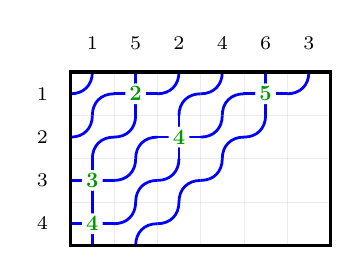
\begin{tikzpicture}[scale=0.55]
  \draw[lightgray, very thin, opacity=0.3] (0,2) -- (6,2);
  \draw[lightgray, very thin, opacity=0.3] (0,3) -- (6,3);
  \draw[lightgray, very thin, opacity=0.3] (0,4) -- (6,4);
  \draw[lightgray, very thin, opacity=0.3] (0,5) -- (6,5);
  \draw[lightgray, very thin, opacity=0.3] (0,6) -- (6,6);
  \draw[lightgray, very thin, opacity=0.3] (0,2) -- (0,6);
  \draw[lightgray, very thin, opacity=0.3] (1,2) -- (1,6);
  \draw[lightgray, very thin, opacity=0.3] (2,2) -- (2,6);
  \draw[lightgray, very thin, opacity=0.3] (3,2) -- (3,6);
  \draw[lightgray, very thin, opacity=0.3] (4,2) -- (4,6);
  \draw[lightgray, very thin, opacity=0.3] (5,2) -- (5,6);
  \draw[lightgray, very thin, opacity=0.3] (6,2) -- (6,6);
  \draw[blue, line width=1.0pt] (0,5.5) .. controls (0.3,5.5) and (0.5,5.7) .. (0.5,6);
  \draw[blue, line width=1.0pt] (0.5,5) .. controls (0.5,5.3) and (0.7,5.5) .. (1,5.5);
  \draw[blue, line width=1.0pt, line cap=round] (1,5.5) -- (2,5.5);
  \draw[blue, line width=1.0pt, line cap=round] (1.5,5) -- (1.5,6);
  \draw[blue, line width=1.0pt] (2,5.5) .. controls (2.3,5.5) and (2.5,5.7) .. (2.5,6);
  \draw[blue, line width=1.0pt] (2.5,5) .. controls (2.5,5.3) and (2.7,5.5) .. (3,5.5);
  \draw[blue, line width=1.0pt] (3,5.5) .. controls (3.3,5.5) and (3.5,5.7) .. (3.5,6);
  \draw[blue, line width=1.0pt] (3.5,5) .. controls (3.5,5.3) and (3.7,5.5) .. (4,5.5);
  \draw[blue, line width=1.0pt, line cap=round] (4,5.5) -- (5,5.5);
  \draw[blue, line width=1.0pt, line cap=round] (4.5,5) -- (4.5,6);
  \draw[blue, line width=1.0pt] (5,5.5) .. controls (5.3,5.5) and (5.5,5.7) .. (5.5,6);
  \draw[blue, line width=1.0pt] (0,4.5) .. controls (0.3,4.5) and (0.5,4.7) .. (0.5,5);
  \draw[blue, line width=1.0pt] (0.5,4) .. controls (0.5,4.3) and (0.7,4.5) .. (1,4.5);
  \draw[blue, line width=1.0pt] (1,4.5) .. controls (1.3,4.5) and (1.5,4.7) .. (1.5,5);
  \draw[blue, line width=1.0pt] (1.5,4) .. controls (1.5,4.3) and (1.7,4.5) .. (2,4.5);
  \draw[blue, line width=1.0pt, line cap=round] (2,4.5) -- (3,4.5);
  \draw[blue, line width=1.0pt, line cap=round] (2.5,4) -- (2.5,5);
  \draw[blue, line width=1.0pt] (3,4.5) .. controls (3.3,4.5) and (3.5,4.7) .. (3.5,5);
  \draw[blue, line width=1.0pt] (3.5,4) .. controls (3.5,4.3) and (3.7,4.5) .. (4,4.5);
  \draw[blue, line width=1.0pt] (4,4.5) .. controls (4.3,4.5) and (4.5,4.7) .. (4.5,5);
  \draw[blue, line width=1.0pt, line cap=round] (0,3.5) -- (1,3.5);
  \draw[blue, line width=1.0pt, line cap=round] (0.5,3) -- (0.5,4);
  \draw[blue, line width=1.0pt] (1,3.5) .. controls (1.3,3.5) and (1.5,3.7) .. (1.5,4);
  \draw[blue, line width=1.0pt] (1.5,3) .. controls (1.5,3.3) and (1.7,3.5) .. (2,3.5);
  \draw[blue, line width=1.0pt] (2,3.5) .. controls (2.3,3.5) and (2.5,3.7) .. (2.5,4);
  \draw[blue, line width=1.0pt] (2.5,3) .. controls (2.5,3.3) and (2.7,3.5) .. (3,3.5);
  \draw[blue, line width=1.0pt] (3,3.5) .. controls (3.3,3.5) and (3.5,3.7) .. (3.5,4);
  \draw[blue, line width=1.0pt, line cap=round] (0,2.5) -- (1,2.5);
  \draw[blue, line width=1.0pt, line cap=round] (0.5,2) -- (0.5,3);
  \draw[blue, line width=1.0pt] (1,2.5) .. controls (1.3,2.5) and (1.5,2.7) .. (1.5,3);
  \draw[blue, line width=1.0pt] (1.5,2) .. controls (1.5,2.3) and (1.7,2.5) .. (2,2.5);
  \draw[blue, line width=1.0pt] (2,2.5) .. controls (2.3,2.5) and (2.5,2.7) .. (2.5,3);
  \node[font=\Large\bfseries, text=green!60!black, fill=white, inner sep=0.5pt, circle, transform shape] at (1.5,5.5) {2};
  \node[font=\Large\bfseries, text=green!60!black, fill=white, inner sep=0.5pt, circle, transform shape] at (4.5,5.5) {5};
  \node[font=\Large\bfseries, text=green!60!black, fill=white, inner sep=0.5pt, circle, transform shape] at (0.5,3.5) {3};
  \node[font=\Large\bfseries, text=green!60!black, fill=white, inner sep=0.5pt, circle, transform shape] at (2.5,4.5) {4};
  \node[font=\Large\bfseries, text=green!60!black, fill=white, inner sep=0.5pt, circle, transform shape] at (0.5,2.5) {4};
  \node[font=\scriptsize, text=black, anchor=south] at (0.5,6.3) {1};
  \node[font=\scriptsize, text=black, anchor=south] at (1.5,6.3) {5};
  \node[font=\scriptsize, text=black, anchor=south] at (2.5,6.3) {2};
  \node[font=\scriptsize, text=black, anchor=south] at (3.5,6.3) {4};
  \node[font=\scriptsize, text=black, anchor=south] at (4.5,6.3) {6};
  \node[font=\scriptsize, text=black, anchor=south] at (5.5,6.3) {3};
  \node[font=\scriptsize, text=black, anchor=east] at (-0.3,5.5) {1};
  \node[font=\scriptsize, text=black, anchor=east] at (-0.3,4.5) {2};
  \node[font=\scriptsize, text=black, anchor=east] at (-0.3,3.5) {3};
  \node[font=\scriptsize, text=black, anchor=east] at (-0.3,2.5) {4};
  \draw[black, line width=1.2000000000000002pt] (0,2) rectangle (6,6);
\end{tikzpicture}}}
  +
  \vcenter{\hbox{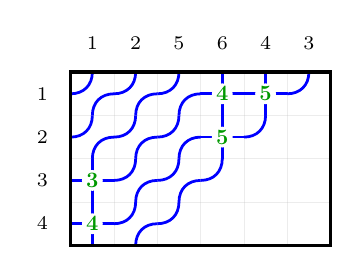
\begin{tikzpicture}[scale=0.55]
  \draw[lightgray, very thin, opacity=0.3] (0,2) -- (6,2);
  \draw[lightgray, very thin, opacity=0.3] (0,3) -- (6,3);
  \draw[lightgray, very thin, opacity=0.3] (0,4) -- (6,4);
  \draw[lightgray, very thin, opacity=0.3] (0,5) -- (6,5);
  \draw[lightgray, very thin, opacity=0.3] (0,6) -- (6,6);
  \draw[lightgray, very thin, opacity=0.3] (0,2) -- (0,6);
  \draw[lightgray, very thin, opacity=0.3] (1,2) -- (1,6);
  \draw[lightgray, very thin, opacity=0.3] (2,2) -- (2,6);
  \draw[lightgray, very thin, opacity=0.3] (3,2) -- (3,6);
  \draw[lightgray, very thin, opacity=0.3] (4,2) -- (4,6);
  \draw[lightgray, very thin, opacity=0.3] (5,2) -- (5,6);
  \draw[lightgray, very thin, opacity=0.3] (6,2) -- (6,6);
  \draw[blue, line width=1.0pt] (0,5.5) .. controls (0.3,5.5) and (0.5,5.7) .. (0.5,6);
  \draw[blue, line width=1.0pt] (0.5,5) .. controls (0.5,5.3) and (0.7,5.5) .. (1,5.5);
  \draw[blue, line width=1.0pt] (1,5.5) .. controls (1.3,5.5) and (1.5,5.7) .. (1.5,6);
  \draw[blue, line width=1.0pt] (1.5,5) .. controls (1.5,5.3) and (1.7,5.5) .. (2,5.5);
  \draw[blue, line width=1.0pt] (2,5.5) .. controls (2.3,5.5) and (2.5,5.7) .. (2.5,6);
  \draw[blue, line width=1.0pt] (2.5,5) .. controls (2.5,5.3) and (2.7,5.5) .. (3,5.5);
  \draw[blue, line width=1.0pt, line cap=round] (3,5.5) -- (4,5.5);
  \draw[blue, line width=1.0pt, line cap=round] (3.5,5) -- (3.5,6);
  \draw[blue, line width=1.0pt, line cap=round] (4,5.5) -- (5,5.5);
  \draw[blue, line width=1.0pt, line cap=round] (4.5,5) -- (4.5,6);
  \draw[blue, line width=1.0pt] (5,5.5) .. controls (5.3,5.5) and (5.5,5.7) .. (5.5,6);
  \draw[blue, line width=1.0pt] (0,4.5) .. controls (0.3,4.5) and (0.5,4.7) .. (0.5,5);
  \draw[blue, line width=1.0pt] (0.5,4) .. controls (0.5,4.3) and (0.7,4.5) .. (1,4.5);
  \draw[blue, line width=1.0pt] (1,4.5) .. controls (1.3,4.5) and (1.5,4.7) .. (1.5,5);
  \draw[blue, line width=1.0pt] (1.5,4) .. controls (1.5,4.3) and (1.7,4.5) .. (2,4.5);
  \draw[blue, line width=1.0pt] (2,4.5) .. controls (2.3,4.5) and (2.5,4.7) .. (2.5,5);
  \draw[blue, line width=1.0pt] (2.5,4) .. controls (2.5,4.3) and (2.7,4.5) .. (3,4.5);
  \draw[blue, line width=1.0pt, line cap=round] (3,4.5) -- (4,4.5);
  \draw[blue, line width=1.0pt, line cap=round] (3.5,4) -- (3.5,5);
  \draw[blue, line width=1.0pt] (4,4.5) .. controls (4.3,4.5) and (4.5,4.7) .. (4.5,5);
  \draw[blue, line width=1.0pt, line cap=round] (0,3.5) -- (1,3.5);
  \draw[blue, line width=1.0pt, line cap=round] (0.5,3) -- (0.5,4);
  \draw[blue, line width=1.0pt] (1,3.5) .. controls (1.3,3.5) and (1.5,3.7) .. (1.5,4);
  \draw[blue, line width=1.0pt] (1.5,3) .. controls (1.5,3.3) and (1.7,3.5) .. (2,3.5);
  \draw[blue, line width=1.0pt] (2,3.5) .. controls (2.3,3.5) and (2.5,3.7) .. (2.5,4);
  \draw[blue, line width=1.0pt] (2.5,3) .. controls (2.5,3.3) and (2.7,3.5) .. (3,3.5);
  \draw[blue, line width=1.0pt] (3,3.5) .. controls (3.3,3.5) and (3.5,3.7) .. (3.5,4);
  \draw[blue, line width=1.0pt, line cap=round] (0,2.5) -- (1,2.5);
  \draw[blue, line width=1.0pt, line cap=round] (0.5,2) -- (0.5,3);
  \draw[blue, line width=1.0pt] (1,2.5) .. controls (1.3,2.5) and (1.5,2.7) .. (1.5,3);
  \draw[blue, line width=1.0pt] (1.5,2) .. controls (1.5,2.3) and (1.7,2.5) .. (2,2.5);
  \draw[blue, line width=1.0pt] (2,2.5) .. controls (2.3,2.5) and (2.5,2.7) .. (2.5,3);
  \node[font=\Large\bfseries, text=green!60!black, fill=white, inner sep=0.5pt, circle, transform shape] at (3.5,4.5) {5};
  \node[font=\Large\bfseries, text=green!60!black, fill=white, inner sep=0.5pt, circle, transform shape] at (4.5,5.5) {5};
  \node[font=\Large\bfseries, text=green!60!black, fill=white, inner sep=0.5pt, circle, transform shape] at (0.5,3.5) {3};
  \node[font=\Large\bfseries, text=green!60!black, fill=white, inner sep=0.5pt, circle, transform shape] at (3.5,5.5) {4};
  \node[font=\Large\bfseries, text=green!60!black, fill=white, inner sep=0.5pt, circle, transform shape] at (0.5,2.5) {4};
  \node[font=\scriptsize, text=black, anchor=south] at (0.5,6.3) {1};
  \node[font=\scriptsize, text=black, anchor=south] at (1.5,6.3) {2};
  \node[font=\scriptsize, text=black, anchor=south] at (2.5,6.3) {5};
  \node[font=\scriptsize, text=black, anchor=south] at (3.5,6.3) {6};
  \node[font=\scriptsize, text=black, anchor=south] at (4.5,6.3) {4};
  \node[font=\scriptsize, text=black, anchor=south] at (5.5,6.3) {3};
  \node[font=\scriptsize, text=black, anchor=east] at (-0.3,5.5) {1};
  \node[font=\scriptsize, text=black, anchor=east] at (-0.3,4.5) {2};
  \node[font=\scriptsize, text=black, anchor=east] at (-0.3,3.5) {3};
  \node[font=\scriptsize, text=black, anchor=east] at (-0.3,2.5) {4};
  \draw[black, line width=1.2000000000000002pt] (0,2) rectangle (6,6);
\end{tikzpicture}}}
  \\[1em]
  + & 
  \vcenter{\hbox{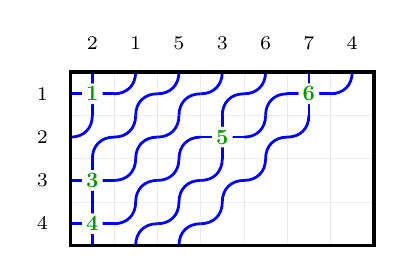
\begin{tikzpicture}[scale=0.55]
  \draw[lightgray, very thin, opacity=0.3] (0,3) -- (7,3);
  \draw[lightgray, very thin, opacity=0.3] (0,4) -- (7,4);
  \draw[lightgray, very thin, opacity=0.3] (0,5) -- (7,5);
  \draw[lightgray, very thin, opacity=0.3] (0,6) -- (7,6);
  \draw[lightgray, very thin, opacity=0.3] (0,7) -- (7,7);
  \draw[lightgray, very thin, opacity=0.3] (0,3) -- (0,7);
  \draw[lightgray, very thin, opacity=0.3] (1,3) -- (1,7);
  \draw[lightgray, very thin, opacity=0.3] (2,3) -- (2,7);
  \draw[lightgray, very thin, opacity=0.3] (3,3) -- (3,7);
  \draw[lightgray, very thin, opacity=0.3] (4,3) -- (4,7);
  \draw[lightgray, very thin, opacity=0.3] (5,3) -- (5,7);
  \draw[lightgray, very thin, opacity=0.3] (6,3) -- (6,7);
  \draw[lightgray, very thin, opacity=0.3] (7,3) -- (7,7);
  \draw[blue, line width=1.0pt, line cap=round] (0,6.5) -- (1,6.5);
  \draw[blue, line width=1.0pt, line cap=round] (0.5,6) -- (0.5,7);
  \draw[blue, line width=1.0pt] (1,6.5) .. controls (1.3,6.5) and (1.5,6.7) .. (1.5,7);
  \draw[blue, line width=1.0pt] (1.5,6) .. controls (1.5,6.3) and (1.7,6.5) .. (2,6.5);
  \draw[blue, line width=1.0pt] (2,6.5) .. controls (2.3,6.5) and (2.5,6.7) .. (2.5,7);
  \draw[blue, line width=1.0pt] (2.5,6) .. controls (2.5,6.3) and (2.7,6.5) .. (3,6.5);
  \draw[blue, line width=1.0pt] (3,6.5) .. controls (3.3,6.5) and (3.5,6.7) .. (3.5,7);
  \draw[blue, line width=1.0pt] (3.5,6) .. controls (3.5,6.3) and (3.7,6.5) .. (4,6.5);
  \draw[blue, line width=1.0pt] (4,6.5) .. controls (4.3,6.5) and (4.5,6.7) .. (4.5,7);
  \draw[blue, line width=1.0pt] (4.5,6) .. controls (4.5,6.3) and (4.7,6.5) .. (5,6.5);
  \draw[blue, line width=1.0pt, line cap=round] (5,6.5) -- (6,6.5);
  \draw[blue, line width=1.0pt, line cap=round] (5.5,6) -- (5.5,7);
  \draw[blue, line width=1.0pt] (6,6.5) .. controls (6.3,6.5) and (6.5,6.7) .. (6.5,7);
  \draw[blue, line width=1.0pt] (0,5.5) .. controls (0.3,5.5) and (0.5,5.7) .. (0.5,6);
  \draw[blue, line width=1.0pt] (0.5,5) .. controls (0.5,5.3) and (0.7,5.5) .. (1,5.5);
  \draw[blue, line width=1.0pt] (1,5.5) .. controls (1.3,5.5) and (1.5,5.7) .. (1.5,6);
  \draw[blue, line width=1.0pt] (1.5,5) .. controls (1.5,5.3) and (1.7,5.5) .. (2,5.5);
  \draw[blue, line width=1.0pt] (2,5.5) .. controls (2.3,5.5) and (2.5,5.7) .. (2.5,6);
  \draw[blue, line width=1.0pt] (2.5,5) .. controls (2.5,5.3) and (2.7,5.5) .. (3,5.5);
  \draw[blue, line width=1.0pt, line cap=round] (3,5.5) -- (4,5.5);
  \draw[blue, line width=1.0pt, line cap=round] (3.5,5) -- (3.5,6);
  \draw[blue, line width=1.0pt] (4,5.5) .. controls (4.3,5.5) and (4.5,5.7) .. (4.5,6);
  \draw[blue, line width=1.0pt] (4.5,5) .. controls (4.5,5.3) and (4.7,5.5) .. (5,5.5);
  \draw[blue, line width=1.0pt] (5,5.5) .. controls (5.3,5.5) and (5.5,5.7) .. (5.5,6);
  \draw[blue, line width=1.0pt, line cap=round] (0,4.5) -- (1,4.5);
  \draw[blue, line width=1.0pt, line cap=round] (0.5,4) -- (0.5,5);
  \draw[blue, line width=1.0pt] (1,4.5) .. controls (1.3,4.5) and (1.5,4.7) .. (1.5,5);
  \draw[blue, line width=1.0pt] (1.5,4) .. controls (1.5,4.3) and (1.7,4.5) .. (2,4.5);
  \draw[blue, line width=1.0pt] (2,4.5) .. controls (2.3,4.5) and (2.5,4.7) .. (2.5,5);
  \draw[blue, line width=1.0pt] (2.5,4) .. controls (2.5,4.3) and (2.7,4.5) .. (3,4.5);
  \draw[blue, line width=1.0pt] (3,4.5) .. controls (3.3,4.5) and (3.5,4.7) .. (3.5,5);
  \draw[blue, line width=1.0pt] (3.5,4) .. controls (3.5,4.3) and (3.7,4.5) .. (4,4.5);
  \draw[blue, line width=1.0pt] (4,4.5) .. controls (4.3,4.5) and (4.5,4.7) .. (4.5,5);
  \draw[blue, line width=1.0pt, line cap=round] (0,3.5) -- (1,3.5);
  \draw[blue, line width=1.0pt, line cap=round] (0.5,3) -- (0.5,4);
  \draw[blue, line width=1.0pt] (1,3.5) .. controls (1.3,3.5) and (1.5,3.7) .. (1.5,4);
  \draw[blue, line width=1.0pt] (1.5,3) .. controls (1.5,3.3) and (1.7,3.5) .. (2,3.5);
  \draw[blue, line width=1.0pt] (2,3.5) .. controls (2.3,3.5) and (2.5,3.7) .. (2.5,4);
  \draw[blue, line width=1.0pt] (2.5,3) .. controls (2.5,3.3) and (2.7,3.5) .. (3,3.5);
  \draw[blue, line width=1.0pt] (3,3.5) .. controls (3.3,3.5) and (3.5,3.7) .. (3.5,4);
  \node[font=\Large\bfseries, text=green!60!black, fill=white, inner sep=0.5pt, circle, transform shape] at (3.5,5.5) {5};
  \node[font=\Large\bfseries, text=green!60!black, fill=white, inner sep=0.5pt, circle, transform shape] at (0.5,4.5) {3};
  \node[font=\Large\bfseries, text=green!60!black, fill=white, inner sep=0.5pt, circle, transform shape] at (0.5,6.5) {1};
  \node[font=\Large\bfseries, text=green!60!black, fill=white, inner sep=0.5pt, circle, transform shape] at (5.5,6.5) {6};
  \node[font=\Large\bfseries, text=green!60!black, fill=white, inner sep=0.5pt, circle, transform shape] at (0.5,3.5) {4};
  \node[font=\scriptsize, text=black, anchor=south] at (0.5,7.3) {2};
  \node[font=\scriptsize, text=black, anchor=south] at (1.5,7.3) {1};
  \node[font=\scriptsize, text=black, anchor=south] at (2.5,7.3) {5};
  \node[font=\scriptsize, text=black, anchor=south] at (3.5,7.3) {3};
  \node[font=\scriptsize, text=black, anchor=south] at (4.5,7.3) {6};
  \node[font=\scriptsize, text=black, anchor=south] at (5.5,7.3) {7};
  \node[font=\scriptsize, text=black, anchor=south] at (6.5,7.3) {4};
  \node[font=\scriptsize, text=black, anchor=east] at (-0.3,6.5) {1};
  \node[font=\scriptsize, text=black, anchor=east] at (-0.3,5.5) {2};
  \node[font=\scriptsize, text=black, anchor=east] at (-0.3,4.5) {3};
  \node[font=\scriptsize, text=black, anchor=east] at (-0.3,3.5) {4};
  \draw[black, line width=1.2000000000000002pt] (0,3) rectangle (7,7);
\end{tikzpicture}}}
  +
  \vcenter{\hbox{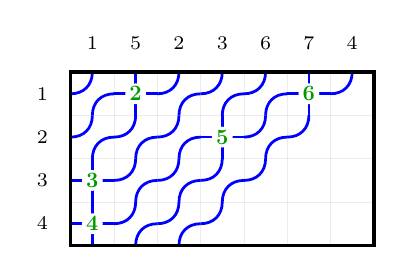
\begin{tikzpicture}[scale=0.55]
  \draw[lightgray, very thin, opacity=0.3] (0,3) -- (7,3);
  \draw[lightgray, very thin, opacity=0.3] (0,4) -- (7,4);
  \draw[lightgray, very thin, opacity=0.3] (0,5) -- (7,5);
  \draw[lightgray, very thin, opacity=0.3] (0,6) -- (7,6);
  \draw[lightgray, very thin, opacity=0.3] (0,7) -- (7,7);
  \draw[lightgray, very thin, opacity=0.3] (0,3) -- (0,7);
  \draw[lightgray, very thin, opacity=0.3] (1,3) -- (1,7);
  \draw[lightgray, very thin, opacity=0.3] (2,3) -- (2,7);
  \draw[lightgray, very thin, opacity=0.3] (3,3) -- (3,7);
  \draw[lightgray, very thin, opacity=0.3] (4,3) -- (4,7);
  \draw[lightgray, very thin, opacity=0.3] (5,3) -- (5,7);
  \draw[lightgray, very thin, opacity=0.3] (6,3) -- (6,7);
  \draw[lightgray, very thin, opacity=0.3] (7,3) -- (7,7);
  \draw[blue, line width=1.0pt] (0,6.5) .. controls (0.3,6.5) and (0.5,6.7) .. (0.5,7);
  \draw[blue, line width=1.0pt] (0.5,6) .. controls (0.5,6.3) and (0.7,6.5) .. (1,6.5);
  \draw[blue, line width=1.0pt, line cap=round] (1,6.5) -- (2,6.5);
  \draw[blue, line width=1.0pt, line cap=round] (1.5,6) -- (1.5,7);
  \draw[blue, line width=1.0pt] (2,6.5) .. controls (2.3,6.5) and (2.5,6.7) .. (2.5,7);
  \draw[blue, line width=1.0pt] (2.5,6) .. controls (2.5,6.3) and (2.7,6.5) .. (3,6.5);
  \draw[blue, line width=1.0pt] (3,6.5) .. controls (3.3,6.5) and (3.5,6.7) .. (3.5,7);
  \draw[blue, line width=1.0pt] (3.5,6) .. controls (3.5,6.3) and (3.7,6.5) .. (4,6.5);
  \draw[blue, line width=1.0pt] (4,6.5) .. controls (4.3,6.5) and (4.5,6.7) .. (4.5,7);
  \draw[blue, line width=1.0pt] (4.5,6) .. controls (4.5,6.3) and (4.7,6.5) .. (5,6.5);
  \draw[blue, line width=1.0pt, line cap=round] (5,6.5) -- (6,6.5);
  \draw[blue, line width=1.0pt, line cap=round] (5.5,6) -- (5.5,7);
  \draw[blue, line width=1.0pt] (6,6.5) .. controls (6.3,6.5) and (6.5,6.7) .. (6.5,7);
  \draw[blue, line width=1.0pt] (0,5.5) .. controls (0.3,5.5) and (0.5,5.7) .. (0.5,6);
  \draw[blue, line width=1.0pt] (0.5,5) .. controls (0.5,5.3) and (0.7,5.5) .. (1,5.5);
  \draw[blue, line width=1.0pt] (1,5.5) .. controls (1.3,5.5) and (1.5,5.7) .. (1.5,6);
  \draw[blue, line width=1.0pt] (1.5,5) .. controls (1.5,5.3) and (1.7,5.5) .. (2,5.5);
  \draw[blue, line width=1.0pt] (2,5.5) .. controls (2.3,5.5) and (2.5,5.7) .. (2.5,6);
  \draw[blue, line width=1.0pt] (2.5,5) .. controls (2.5,5.3) and (2.7,5.5) .. (3,5.5);
  \draw[blue, line width=1.0pt, line cap=round] (3,5.5) -- (4,5.5);
  \draw[blue, line width=1.0pt, line cap=round] (3.5,5) -- (3.5,6);
  \draw[blue, line width=1.0pt] (4,5.5) .. controls (4.3,5.5) and (4.5,5.7) .. (4.5,6);
  \draw[blue, line width=1.0pt] (4.5,5) .. controls (4.5,5.3) and (4.7,5.5) .. (5,5.5);
  \draw[blue, line width=1.0pt] (5,5.5) .. controls (5.3,5.5) and (5.5,5.7) .. (5.5,6);
  \draw[blue, line width=1.0pt, line cap=round] (0,4.5) -- (1,4.5);
  \draw[blue, line width=1.0pt, line cap=round] (0.5,4) -- (0.5,5);
  \draw[blue, line width=1.0pt] (1,4.5) .. controls (1.3,4.5) and (1.5,4.7) .. (1.5,5);
  \draw[blue, line width=1.0pt] (1.5,4) .. controls (1.5,4.3) and (1.7,4.5) .. (2,4.5);
  \draw[blue, line width=1.0pt] (2,4.5) .. controls (2.3,4.5) and (2.5,4.7) .. (2.5,5);
  \draw[blue, line width=1.0pt] (2.5,4) .. controls (2.5,4.3) and (2.7,4.5) .. (3,4.5);
  \draw[blue, line width=1.0pt] (3,4.5) .. controls (3.3,4.5) and (3.5,4.7) .. (3.5,5);
  \draw[blue, line width=1.0pt] (3.5,4) .. controls (3.5,4.3) and (3.7,4.5) .. (4,4.5);
  \draw[blue, line width=1.0pt] (4,4.5) .. controls (4.3,4.5) and (4.5,4.7) .. (4.5,5);
  \draw[blue, line width=1.0pt, line cap=round] (0,3.5) -- (1,3.5);
  \draw[blue, line width=1.0pt, line cap=round] (0.5,3) -- (0.5,4);
  \draw[blue, line width=1.0pt] (1,3.5) .. controls (1.3,3.5) and (1.5,3.7) .. (1.5,4);
  \draw[blue, line width=1.0pt] (1.5,3) .. controls (1.5,3.3) and (1.7,3.5) .. (2,3.5);
  \draw[blue, line width=1.0pt] (2,3.5) .. controls (2.3,3.5) and (2.5,3.7) .. (2.5,4);
  \draw[blue, line width=1.0pt] (2.5,3) .. controls (2.5,3.3) and (2.7,3.5) .. (3,3.5);
  \draw[blue, line width=1.0pt] (3,3.5) .. controls (3.3,3.5) and (3.5,3.7) .. (3.5,4);
  \node[font=\Large\bfseries, text=green!60!black, fill=white, inner sep=0.5pt, circle, transform shape] at (3.5,5.5) {5};
  \node[font=\Large\bfseries, text=green!60!black, fill=white, inner sep=0.5pt, circle, transform shape] at (1.5,6.5) {2};
  \node[font=\Large\bfseries, text=green!60!black, fill=white, inner sep=0.5pt, circle, transform shape] at (0.5,4.5) {3};
  \node[font=\Large\bfseries, text=green!60!black, fill=white, inner sep=0.5pt, circle, transform shape] at (5.5,6.5) {6};
  \node[font=\Large\bfseries, text=green!60!black, fill=white, inner sep=0.5pt, circle, transform shape] at (0.5,3.5) {4};
  \node[font=\scriptsize, text=black, anchor=south] at (0.5,7.3) {1};
  \node[font=\scriptsize, text=black, anchor=south] at (1.5,7.3) {5};
  \node[font=\scriptsize, text=black, anchor=south] at (2.5,7.3) {2};
  \node[font=\scriptsize, text=black, anchor=south] at (3.5,7.3) {3};
  \node[font=\scriptsize, text=black, anchor=south] at (4.5,7.3) {6};
  \node[font=\scriptsize, text=black, anchor=south] at (5.5,7.3) {7};
  \node[font=\scriptsize, text=black, anchor=south] at (6.5,7.3) {4};
  \node[font=\scriptsize, text=black, anchor=east] at (-0.3,6.5) {1};
  \node[font=\scriptsize, text=black, anchor=east] at (-0.3,5.5) {2};
  \node[font=\scriptsize, text=black, anchor=east] at (-0.3,4.5) {3};
  \node[font=\scriptsize, text=black, anchor=east] at (-0.3,3.5) {4};
  \draw[black, line width=1.2000000000000002pt] (0,3) rectangle (7,7);
\end{tikzpicture}}}
  +
  \vcenter{\hbox{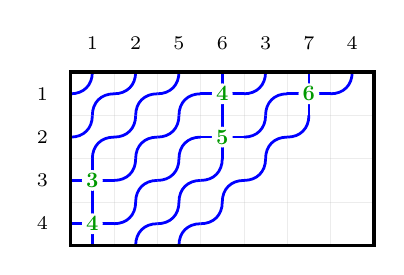
\begin{tikzpicture}[scale=0.55]
  \draw[lightgray, very thin, opacity=0.3] (0,3) -- (7,3);
  \draw[lightgray, very thin, opacity=0.3] (0,4) -- (7,4);
  \draw[lightgray, very thin, opacity=0.3] (0,5) -- (7,5);
  \draw[lightgray, very thin, opacity=0.3] (0,6) -- (7,6);
  \draw[lightgray, very thin, opacity=0.3] (0,7) -- (7,7);
  \draw[lightgray, very thin, opacity=0.3] (0,3) -- (0,7);
  \draw[lightgray, very thin, opacity=0.3] (1,3) -- (1,7);
  \draw[lightgray, very thin, opacity=0.3] (2,3) -- (2,7);
  \draw[lightgray, very thin, opacity=0.3] (3,3) -- (3,7);
  \draw[lightgray, very thin, opacity=0.3] (4,3) -- (4,7);
  \draw[lightgray, very thin, opacity=0.3] (5,3) -- (5,7);
  \draw[lightgray, very thin, opacity=0.3] (6,3) -- (6,7);
  \draw[lightgray, very thin, opacity=0.3] (7,3) -- (7,7);
  \draw[blue, line width=1.0pt] (0,6.5) .. controls (0.3,6.5) and (0.5,6.7) .. (0.5,7);
  \draw[blue, line width=1.0pt] (0.5,6) .. controls (0.5,6.3) and (0.7,6.5) .. (1,6.5);
  \draw[blue, line width=1.0pt] (1,6.5) .. controls (1.3,6.5) and (1.5,6.7) .. (1.5,7);
  \draw[blue, line width=1.0pt] (1.5,6) .. controls (1.5,6.3) and (1.7,6.5) .. (2,6.5);
  \draw[blue, line width=1.0pt] (2,6.5) .. controls (2.3,6.5) and (2.5,6.7) .. (2.5,7);
  \draw[blue, line width=1.0pt] (2.5,6) .. controls (2.5,6.3) and (2.7,6.5) .. (3,6.5);
  \draw[blue, line width=1.0pt, line cap=round] (3,6.5) -- (4,6.5);
  \draw[blue, line width=1.0pt, line cap=round] (3.5,6) -- (3.5,7);
  \draw[blue, line width=1.0pt] (4,6.5) .. controls (4.3,6.5) and (4.5,6.7) .. (4.5,7);
  \draw[blue, line width=1.0pt] (4.5,6) .. controls (4.5,6.3) and (4.7,6.5) .. (5,6.5);
  \draw[blue, line width=1.0pt, line cap=round] (5,6.5) -- (6,6.5);
  \draw[blue, line width=1.0pt, line cap=round] (5.5,6) -- (5.5,7);
  \draw[blue, line width=1.0pt] (6,6.5) .. controls (6.3,6.5) and (6.5,6.7) .. (6.5,7);
  \draw[blue, line width=1.0pt] (0,5.5) .. controls (0.3,5.5) and (0.5,5.7) .. (0.5,6);
  \draw[blue, line width=1.0pt] (0.5,5) .. controls (0.5,5.3) and (0.7,5.5) .. (1,5.5);
  \draw[blue, line width=1.0pt] (1,5.5) .. controls (1.3,5.5) and (1.5,5.7) .. (1.5,6);
  \draw[blue, line width=1.0pt] (1.5,5) .. controls (1.5,5.3) and (1.7,5.5) .. (2,5.5);
  \draw[blue, line width=1.0pt] (2,5.5) .. controls (2.3,5.5) and (2.5,5.7) .. (2.5,6);
  \draw[blue, line width=1.0pt] (2.5,5) .. controls (2.5,5.3) and (2.7,5.5) .. (3,5.5);
  \draw[blue, line width=1.0pt, line cap=round] (3,5.5) -- (4,5.5);
  \draw[blue, line width=1.0pt, line cap=round] (3.5,5) -- (3.5,6);
  \draw[blue, line width=1.0pt] (4,5.5) .. controls (4.3,5.5) and (4.5,5.7) .. (4.5,6);
  \draw[blue, line width=1.0pt] (4.5,5) .. controls (4.5,5.3) and (4.7,5.5) .. (5,5.5);
  \draw[blue, line width=1.0pt] (5,5.5) .. controls (5.3,5.5) and (5.5,5.7) .. (5.5,6);
  \draw[blue, line width=1.0pt, line cap=round] (0,4.5) -- (1,4.5);
  \draw[blue, line width=1.0pt, line cap=round] (0.5,4) -- (0.5,5);
  \draw[blue, line width=1.0pt] (1,4.5) .. controls (1.3,4.5) and (1.5,4.7) .. (1.5,5);
  \draw[blue, line width=1.0pt] (1.5,4) .. controls (1.5,4.3) and (1.7,4.5) .. (2,4.5);
  \draw[blue, line width=1.0pt] (2,4.5) .. controls (2.3,4.5) and (2.5,4.7) .. (2.5,5);
  \draw[blue, line width=1.0pt] (2.5,4) .. controls (2.5,4.3) and (2.7,4.5) .. (3,4.5);
  \draw[blue, line width=1.0pt] (3,4.5) .. controls (3.3,4.5) and (3.5,4.7) .. (3.5,5);
  \draw[blue, line width=1.0pt] (3.5,4) .. controls (3.5,4.3) and (3.7,4.5) .. (4,4.5);
  \draw[blue, line width=1.0pt] (4,4.5) .. controls (4.3,4.5) and (4.5,4.7) .. (4.5,5);
  \draw[blue, line width=1.0pt, line cap=round] (0,3.5) -- (1,3.5);
  \draw[blue, line width=1.0pt, line cap=round] (0.5,3) -- (0.5,4);
  \draw[blue, line width=1.0pt] (1,3.5) .. controls (1.3,3.5) and (1.5,3.7) .. (1.5,4);
  \draw[blue, line width=1.0pt] (1.5,3) .. controls (1.5,3.3) and (1.7,3.5) .. (2,3.5);
  \draw[blue, line width=1.0pt] (2,3.5) .. controls (2.3,3.5) and (2.5,3.7) .. (2.5,4);
  \draw[blue, line width=1.0pt] (2.5,3) .. controls (2.5,3.3) and (2.7,3.5) .. (3,3.5);
  \draw[blue, line width=1.0pt] (3,3.5) .. controls (3.3,3.5) and (3.5,3.7) .. (3.5,4);
  \node[font=\Large\bfseries, text=green!60!black, fill=white, inner sep=0.5pt, circle, transform shape] at (3.5,5.5) {5};
  \node[font=\Large\bfseries, text=green!60!black, fill=white, inner sep=0.5pt, circle, transform shape] at (0.5,4.5) {3};
  \node[font=\Large\bfseries, text=green!60!black, fill=white, inner sep=0.5pt, circle, transform shape] at (3.5,6.5) {4};
  \node[font=\Large\bfseries, text=green!60!black, fill=white, inner sep=0.5pt, circle, transform shape] at (5.5,6.5) {6};
  \node[font=\Large\bfseries, text=green!60!black, fill=white, inner sep=0.5pt, circle, transform shape] at (0.5,3.5) {4};
  \node[font=\scriptsize, text=black, anchor=south] at (0.5,7.3) {1};
  \node[font=\scriptsize, text=black, anchor=south] at (1.5,7.3) {2};
  \node[font=\scriptsize, text=black, anchor=south] at (2.5,7.3) {5};
  \node[font=\scriptsize, text=black, anchor=south] at (3.5,7.3) {6};
  \node[font=\scriptsize, text=black, anchor=south] at (4.5,7.3) {3};
  \node[font=\scriptsize, text=black, anchor=south] at (5.5,7.3) {7};
  \node[font=\scriptsize, text=black, anchor=south] at (6.5,7.3) {4};
  \node[font=\scriptsize, text=black, anchor=east] at (-0.3,6.5) {1};
  \node[font=\scriptsize, text=black, anchor=east] at (-0.3,5.5) {2};
  \node[font=\scriptsize, text=black, anchor=east] at (-0.3,4.5) {3};
  \node[font=\scriptsize, text=black, anchor=east] at (-0.3,3.5) {4};
  \draw[black, line width=1.2000000000000002pt] (0,3) rectangle (7,7);
\end{tikzpicture}}}
\end{align*}


\end{example}


% \subsection{Generating the RC graph ring}
% \newcommand{\BRCC}{\overline{\BRC}}
% % multiplying by empty row ordering
% We enlarge the module $\BRC$ to include bounded RC graphs $R$ with $\hr(R)=n$ that do not necessarily satisfy the condition that $\maxd(\wof{R})\leq n$, only that $R$ has at most $n$ rows. We denote this larger module by $\BRCC$. For $(R, p)\in \BRCC$, define $(R, p)^T\in \BRC$ by $(R^T,\maxd(\wof{R}^{-1}))$. We may define an associative product on $\BRCC$ by
% $$(R_1, p)\spadesuit(R_2,q) = \mathtt{sz}_{p+q}(((R_1, p)^T\sqcupplus (R_2, q)^T)^T)$$
% where $\mathtt{sz}_n:\BRCC\to \BRCC$ is defined on basis elements by 
% $$\mathtt{sz}_n(R, m) = \begin{cases}(R, n) & \text{if } i\leq n\text{ for all }(i, j)\in R\\
% 0 & \text{otherwise}\end{cases}$$
\subsection{Proof of the Littlewood-Richardson rule for the dual Schubert basis}

We first need a formula for a monomial in $\dcoma$ in terms of the dual Schubert basis. This is given by the following lemma, which is a direct consequence of the definition of the dual Schubert polynomials.

\begin{lemma} \label{lemma:sumform}
Let $a$ be a weak composition of length $n$. Then in $\dcoma$ we have
$$[a] = \sum_{\wtt(W)=a}\dsch_{\wof{W}}^{\hr(W)}.$$
\end{lemma}
\begin{proof}
Collecting coefficients, the coefficient of $\dsch_w^n$ on the right-hand side is the number of RC graphs $W$ with $\wof{W}=w$, $\hr(W)=n$, and $\wtt(W)=a$. By definition, this coefficient is the coefficient of the monomial $x^a$ in $\dsch_w^n$, which is equal to $\langle \sch_w^n, [a]\rangle$.
\end{proof}

\begin{definition}
Let $\mathcal{R}$  be the subring of $\BRC$ generated by the single-row RC graphs $\mathtt{row}(i)$ for $i\geq 0$. Let $a$ be a sequence of elements of a ring indexed by the nonnegative integers. For a permutation $w$ and an integer $n\geq \maxd(w)$, define a function $\dsch_w^n(a)$ by
$$\dsch_w^n(a) = \sum_{\alpha} d_{\alpha, w}^n a_{\alpha_1} \cdots a_{\alpha_n}$$
where the sum is over all weak compositions $\alpha$ of length $n$, and $d_{\alpha, w}^n$ is the coefficient of $\alpha$ in $\dsch_w^n\in\dcoma$.
\end{definition}

\begin{lemma} \label{lemma:schubertrow}
We have that the elements
$$\dsch_w^n(\mathtt{row})$$
for integers $n\geq 0$ and $w$ that ranges over all permutations in $S_\infty$ with $n\geq \maxd(w)$ form a $\mathbb{Z}$-basis of $\mathcal{R}$, and $\alpha|\mathcal{R}:\mathcal{R}\to \dcoma$ is an isomorphism of graded rings.
\end{lemma}
\begin{proof}
Define a ring homomorphism $\iota:\dcoma\to \mathcal{R}$ by sending $[a]$ to the RC graph $\mathtt{row}(a)$, which is a homomorphism because $\dcoma$ is free on these generators, and is surjective by definition of $\mathcal{R}$. Then for a weak composition $a$,
$$\iota([a]) = \sum_{\wtt(R)=a} R.$$
Applying $\alpha$ to this sum gives
$$\alpha(\iota([a])) = \sum_{\wtt(R)=a}\dsch_{\wof{R}}^{\hr(R)} = [a]$$
by Lemma \ref{lemma:sumform}. Being the inverse of the surjective homomorphism $\iota$, $\alpha|\mathcal{R}$ is an isomorphism of rings.

Finally, the family $\{\dsch_w^n\}_{n\ge 0,\, n\ge\maxd(w)}$ is a $\mathbb{Z}$-basis of $\dcoma$ by construction, and
$$
\alpha\bigl(\dsch_w^n(\mathtt{row})\bigr)=\dsch_w^n.
$$
Applying the inverse isomorphism $\iota$ shows that $\{\dsch_w^n(\mathtt{row})\}$ is a $\mathbb{Z}$-basis of $\mathcal{R}$.
\end{proof}

We isolate first a structural feature of $\sqcupplus$ that will be used repeatedly here and in Sections \ref{section:crystals}--\ref{section:slide}. It says that in a product $A\sqcupplus W$ the second factor enters only as an inert block of rows sitting below a collection of top blocks determined by $A$ and by the permutation of $W$ alone.

\begin{lemma}[Block decomposition of $\sqcupplus$]\label{lemma:blockdecomp}
Let $A$ and $W$ be bounded RC graphs with $\hr(A)=k$ and $\hr(W)=m$. Then
$$A\sqcupplus W=\sum_{A'}\bigl(A'\cup\shup^{k}W\bigr),$$
each term occurring with multiplicity one and understood to have $k+m$ rows, where $A'$ ranges over the RC graphs all of whose crossings lie in rows $1,\ldots,k$ and which satisfy the two conditions
\begin{enumerate}
\item $\clp^{k}(A')=A$, where $A'$ is regarded as having $\max\{k+m,\maxd(\wof{A'})\}$ rows, and
\item $\ell\bigl(\wof{A'}\shup^{k}\wof W\bigr)=\ell(\wof{A'})+\ell(\wof W)$ and $\maxd\bigl(\wof{A'}\shup^{k}\wof W\bigr)\leq k+m$.
\end{enumerate}
In particular the set of $A'$ being summed over depends on $W$ only through the permutation $\wof W$.
\end{lemma}
\begin{proof}
By Definition \ref{definition:ringproduct}, the terms of $A\sqcupplus W$ are the bounded RC graphs $R$ with $\hr(R)=k+m$, $\clp^{k}(R)=A$ and $\trm^{k}(R)=W$. The condition on the trim says exactly that the crossings of $R$ in rows $k+1,\ldots,k+m$ are those of $\shup^{k}W$; hence $R=A'\cup\shup^{k}W$, where $A'=\{(i,j)\in R\mid i\leq k\}$, and conversely $A'$ determines $R$. So the assignment $R\mapsto A'$ is a bijection onto its image and all multiplicities are $1$.

By Lemma \ref{lemma:cliplocal}, $\clp^{k}(R)$ depends only on $A'$ and not on $\hr(R)$, so the condition $\clp^{k}(R)=A$ is precisely condition (1), a condition on $A'$ alone. Finally, $R$ is a bounded RC graph with $k+m$ rows if and only if the concatenation of $\mathrm{word}(A')$ with $\mathrm{word}(W)$ shifted up by $k$ is reduced and the resulting permutation has last descent at most $k+m$. Since that permutation is $\wof{A'}\shup^{k}\wof{W}$, this is condition (2), which involves $W$ only through $\wof W$.
\end{proof}

\begin{corollary}[Swapping the lower block]\label{corollary:blockswap}
Let $A$, $W_1$ and $W_2$ be bounded RC graphs with $\hr(A)=k$, $\hr(W_1)=\hr(W_2)=m$ and $\wof{W_1}=\wof{W_2}$. Then
$$A'\cup\shup^{k}W_1\ \longmapsto\ A'\cup\shup^{k}W_2$$
is a bijection from the set of terms of $A\sqcupplus W_1$ onto the set of terms of $A\sqcupplus W_2$. Corresponding terms have identical crossings in rows $1,\ldots,k$, have the same permutation, and have words
$$\mathrm{word}(A')\cdot\bigl(\mathrm{word}(W_1)+k\bigr)\quad\text{and}\quad \mathrm{word}(A')\cdot\bigl(\mathrm{word}(W_2)+k\bigr)$$
respectively, where $+k$ denotes adding $k$ to every letter.
\end{corollary}
\begin{proof}
Immediate from Lemma \ref{lemma:blockdecomp}, since the two products are summed over the same set of $A'$. The statement about words holds because the crossing $(i,j)$ of $W_r$ contributes the letter $i+j-1$ to $\mathrm{word}(W_r)$ while the crossing $(i+k,j)$ of $\shup^{k}W_r$ contributes the letter $i+j-1+k$, and because the crossings of rows $1,\ldots,k$ precede those of rows $k+1,\ldots,k+m$ in the order of Definition \ref{definition:rcgraph}.
\end{proof}

Applying Lemma \ref{lemma:blockdecomp} with the roles of the two factors interchanged decomposes a product $W\sqcupplus A$ over the RC graphs $B$ occupying its top $m$ rows, subject to $\clp^{m}(B)=W$ together with a validity condition depending on $B$ only through $\wof B$. This is what lets one vary the top factor, and the following lemma packages it together with the bijection that does the varying.

\begin{lemma}[Matching the top blocks]\label{lemma:topmatch}
Let $W_1$ and $W_2$ be bounded RC graphs with $\hr(W_1)=\hr(W_2)=m$ and $\wof{W_1}=\wof{W_2}$. For $r=1,2$, call an RC graph $B$ \emph{admissible for $W_r$} if all of its crossings lie in rows $1,\ldots,m$ and $\clp^{m}(B)=W_r$, where $B$ is regarded as having $\max\{m,\maxd(\wof B)\}$ rows. Then for each permutation $w'$ there is at most one $B$ admissible for $W_1$ with $\wof B=w'$, and such a $B$ exists if and only if there is a (necessarily unique) $B'$ admissible for $W_2$ with $\wof{B'}=w'$. Writing $\beta(B)=B'$ for the resulting bijection, we have:
\begin{enumerate}
\item $\wof{\beta(B)}=\wof B$ for every $B$ admissible for $W_1$;
\item for every bounded RC graph $A$ with $\hr(A)=k$, the assignment
$$B\cup\shup^{m}A\ \longmapsto\ \beta(B)\cup\shup^{m}A$$
is a bijection from the set of terms of $W_1\sqcupplus A$ onto the set of terms of $W_2\sqcupplus A$, and corresponding terms have the same permutation and have words
$$\mathrm{word}(B)\cdot\bigl(\mathrm{word}(A)+m\bigr)\quad\text{and}\quad\mathrm{word}(\beta(B))\cdot\bigl(\mathrm{word}(A)+m\bigr);$$
\item $\beta$ is the composite of the $\max\{m,\maxd(w')\}-m$ single-row bijections supplied by Theorem \ref{theorem:zero_bijection}, in the sense that $\clp^{m}$ carries $B$ to $W_1$ and $\beta(B)$ to $W_2$ through the same number of applications of $\zeromap$.
\end{enumerate}
\end{lemma}
\begin{proof}
Fix a permutation $w'$ and set $h=\max\{m,\maxd(w')\}$. An RC graph $B$ admissible for $W_r$ with $\wof B=w'$ is precisely an element of $\RC_h(w')$ whose rows $m+1,\ldots,h$ are empty and which satisfies $\zeromap^{\,h-m}(B)=W_r$, by Definition \ref{definition:clptrm}. Each application of $\zeromap$ is injective on the graphs of a fixed permutation with empty last row by Lemma \ref{lemma:zero_surjective}, and distinct graphs with distinct permutations remain distinct; hence $\zeromap^{\,h-m}$ is injective on this set, giving the asserted uniqueness. By Theorem \ref{theorem:zero_bijection} each application of $\zeromap$ is moreover a bijection onto $\bigcup_{w\downvar{}w''}\RC(w'')$, so such a $B$ exists if and only if $W_r$ is reachable from $w'$ by $h-m$ transition steps, a condition depending only on $\wof{W_r}$. As $\wof{W_1}=\wof{W_2}$, the two existence conditions agree, which gives the bijection $\beta$ and assertions (1) and (3).

For (2), apply Lemma \ref{lemma:blockdecomp} with $W_r$ in the role of the first factor and $A$ in the role of the second. Its condition (1) says exactly that $B$ is admissible for $W_r$, and its condition (2) constrains $B$ only through $\wof B$ and $\wof A$. Since $\wof{\beta(B)}=\wof B$, the bijection $\beta$ therefore restricts to a bijection between the two sets of terms. The claims about permutations and words are those of Corollary \ref{corollary:blockswap}, read with the factors interchanged.
\end{proof}

\begin{definition}\label{definition:omega}
Let $\Omega$ be the $\mathbb{Z}$-submodule of $\BRC$ generated by the RC graphs $R_1-R_2$ such that $\wof{R_1}=\wof{R_2}$ and $\hr(R_1)=\hr(R_2)$.
\end{definition}

\begin{lemma}
$\Omega$ is a two-sided ideal of $\BRC$.
\end{lemma}
\begin{proof}
Let $W_1-W_2$ be a generator of $\Omega$, so that $\wof{W_1}=\wof{W_2}$ and $\hr(W_1)=\hr(W_2)=m$, and let $A$ be a bounded RC graph with $\hr(A)=k$.

For the left ideal property, Corollary \ref{corollary:blockswap} matches the terms of $A\sqcupplus W_1$ with those of $A\sqcupplus W_2$ so that corresponding terms have the same permutation, and both have $k+m$ rows. Hence $A\sqcupplus(W_1-W_2)$ is a sum of differences of pairs of bounded RC graphs each agreeing in permutation and number of rows, each with coefficient $1$, so it lies in $\Omega$.

For the right ideal property, Lemma \ref{lemma:topmatch}(2) matches the terms of $W_1\sqcupplus A$ with those of $W_2\sqcupplus A$, and by Lemma \ref{lemma:topmatch}(1) corresponding terms again have the same permutation and the same number of rows. Hence $(W_1-W_2)\sqcupplus A\in\Omega$, and $\Omega$ is a two-sided ideal of $\BRC$.
\end{proof}

\begin{theorem} \label{theorem:semidirect}
  We have that $\alpha:\BRC\to \dcoma$ is a surjective homomorphism of rings with kernel $\Omega$, and the homomorphism $\iota:\dcoma\to\BRC$ sending $[i]\mapsto \mathtt{row}(i)$ is a right inverse to $\alpha$. In particular, $\BRC\cong \dcoma\ltimes \Omega$ as rings.
\end{theorem}
\begin{proof}
  For RC graphs $R_1,R_2$, we have that $\alpha(R_1)=\alpha(R_2)$ if and only if $\wof{R_1}=\wof{R_2}$ and $\hr(R_1)=\hr(R_2)$. Therefore the kernel of $\alpha$ is precisely $\Omega$. Since $\Omega$ is a two-sided ideal, we can conclude that $\alpha$ is in fact a homomorphism of rings. We thus have an exact sequence of ring homomorphisms
$$0\to \Omega\to \BRC\to \dcoma\to 0$$
where the map $\BRC\to \dcoma$ is $\alpha$. We have a homomorphism $\iota:\dcoma\to \BRC$ sending $[i]\mapsto \mathtt{row}(i)$ inducing an isomorphism on $\mathcal{R}$ by Lemma \ref{lemma:schubertrow}, and the composition $\dcoma\to \BRC\to \dcoma$ is the identity since $\alpha(\mathtt{row}(i)) = [i]$.  By virtue of the existence of the section $\iota$, we have that $\BRC = \mathcal{R}\oplus \Omega$, and $\mathcal{R}\cong \dcoma$, we have $\BRC\cong \dcoma\ltimes \Omega$ as rings.
\end{proof}

% \begin{proposition}
% Let $[c]$ be a weak composition of length $n$. Then
% $$[c] = \sum_{\substack{w\in S_\infty\\\maxd(w)\leq n}}\#{R\in \RC_n(w)\mid wtt(R)=c} \dsch_{\wof{R}}^n$$
% \end{proposition}


\begin{definition}
Given RC graphs $U\in \RC_p(u)$ and $V\in\RC_q(v)$ and a permutation $w$, define
$$d_{U, V}^w = \#\{R\in \RC_{p+q}(w): \clp^p(R)=U,\trm^p(R)=V\}$$
\end{definition}

\begin{proof}[Proof of Theorem \ref{theorem:LR}]
Fix $u,v\in S_\infty$ with last descents at most $p,q$ respectively. The element
$$\dsch_u^p\sqcupplus\dsch_v^q\;\in\;\dcoma_{p+q}$$
depends only on $u,v,p,q$, so its expansion coefficients $d_{u,v}^w(p,q)$ in the dual Schubert basis are well defined and \emph{a priori} independent of any auxiliary RC-graph choices.

Choose any $U\in\RC_p(u)$ and $V\in\RC_q(v)$; such graphs exist because $u$ and $v$ have last descents at most $p$ and $q$. By definition of $\alpha$,
$$\alpha(U)=\dsch_u^p,\qquad \alpha(V)=\dsch_v^q.$$
By Theorem \ref{theorem:semidirect}, $\alpha:\BRC\to\dcoma$ is a ring homomorphism, hence
$$\dsch_u^p\sqcupplus\dsch_v^q\;=\;\alpha(U)\sqcupplus\alpha(V)\;=\;\alpha\bigl(U\sqcupplus V\bigr).$$
By the definition of $\sqcupplus$ on $\BRC$,
$$U\sqcupplus V\;=\;\sum_{\substack{R\in\RC_{p+q}\\ \clp^p(R)=U,\ \trm^p(R)=V}} R,$$
and applying $\alpha$ termwise,
\begin{equation}\label{eq:LRexpansion}
\dsch_u^p\sqcupplus\dsch_v^q\;=\;\sum_{\substack{R\in\RC_{p+q}\\ \clp^p(R)=U,\ \trm^p(R)=V}}\dsch_{\wof{R}}^{p+q}.
\end{equation}
The dual Schubert polynomials $\{\dsch_w^{p+q}\}_{\maxd(w)\leq p+q}$ are linearly independent in $\dcoma_{p+q}$. Comparing coefficients of $\dsch_w^{p+q}$ in \eqref{eq:LRexpansion} with the defining expansion
$$\dsch_u^p\sqcupplus\dsch_v^q\;=\;\sum_w d_{u,v}^w(p,q)\,\dsch_w^{p+q}$$
yields
$$d_{u,v}^w(p,q)\;=\;d_{U,V}^w\;=\;\#\bigl\{R\in\RC_{p+q}(w):\clp^p(R)=U,\ \trm^p(R)=V\bigr\}.$$
Since the LHS is independent of the choices of $U,V$, so is the RHS; this gives the theorem and shows in particular that $d_{u,v}^w(p,q)\in\mathbb{Z}_{\geq 0}$.
\end{proof}

% Let $R$ be an RC graph with $\wof{R}=w$ and $\hr(R)=n$. Then for any $m\leq n$,
% $$\dsch_w^n = \alpha(\clp^m(R))\alpha(\trm^m(R)) - \sum_{\substack{\clp^m(R')=\clp^m(R)\\\trm^m(R')=\trm^m(R)\\R'\neq R}} \alpha(R')$$

% $n=4$

% $$\dsch_w^4 = \alpha(\clp^2(R))\alpha(\trm^2(R)) - \sum_{R'}\alpha(\clp^1(R))\alpha(\trm^1(R'))$$

% $$\dsch_w^m = \sum_i(-1)^{i-1}\sum_{\substack{\clp^{\left\lfloor \frac m{2^{i}}\right\rfloor}(R')=\clp^{\left\lfloor \frac m{2^{i}}\right\rfloor}(R)\\\trm^{\left\lfloor \frac m{2^{i}}\right\rfloor}(R')=\trm^{\left\lfloor \frac m{2^{i}}\right\rfloor}(R)\\\trm^{\left\lfloor \frac m{2^{i+1}}\right\rfloor}(R')\neq\trm^{\left\lfloor \frac m{2^{i+1}}\right\rfloor}(R)}} \alpha(\clp^{\left\lfloor \frac m{2^i}\right\rfloor}(R))\alpha(\trm^{\left\lfloor \frac m{2^i}\right\rfloor}(R'))$$

% Suppose $D\in \dcoma$ satisfies
% $$D = \sum_{w} c_w \dsch_w^n$$
% Then
% $$D = \sum_{w} c_w \wtt(\dsch_w^n(\mathtt{row}))$$

\section{The ring of RC graph crystals}\label{section:crystals}

The key polynomials $\kappa_a$ (also called \emph{Demazure characters} in type $A$) form a $\mathbb{Z}$-basis of $\mathbb{Z}[x_1,x_2,\ldots]$ indexed by weak compositions $a$. Their origin lies in the work of Demazure \cite{demazure1974desingularisation,demazure1974nouvelle}, who introduced isobaric divided difference operators $\pi_i$ in order to compute the characters of the $B$-modules $H^0(X_w,\mathcal{L}_\lambda)$ associated to Schubert varieties $X_w$ in $G/B$. In type $A$, the resulting characters become polynomials in the $x_i$, and one obtains $\kappa_a$ for any weak composition $a$ by setting $\kappa_\lambda = x^\lambda$ when $\lambda$ is a partition (a dominant weight) and applying the appropriate operator $\pi_i$ at each descent of $a$ to interpolate between rearrangements of $\lambda$.

A purely combinatorial development of key polynomials was carried out by Lascoux and Schützenberger \cite{lascoux1990keys}, who introduced the \emph{right key} $K_+(T)$ and \emph{left key} $K_-(T)$ of a semistandard Young tableau $T$ and proved that
$$\kappa_a = \sum_{T} x^{\wtt(T)},$$
where the sum runs over semistandard Young tableaux $T$ of shape $\mathrm{sort}(a)$ whose right key $K_+(T)$ is bounded above (entrywise) by the key tableau associated to $a$. They additionally proved that Schubert polynomials decompose as a positive sum of key polynomials, given a combinatorial proof in terms of compatible sequences and the right-key map by Reiner and Shimozono \cite{reiner1995key}. The intermediate basis of \emph{Demazure atoms} (the ``standard bases'' of \cite{lascoux1990keys}) was later given an explicit nonnegative monomial expansion by Mason \cite{mason2009explicit} via semi-skyline augmented fillings.

From a representation-theoretic perspective, Kashiwara \cite{kashiwara1993crystal} introduced \emph{Demazure crystals}: for a dominant integral weight $\lambda$ with crystal $B(\lambda)$ and a Weyl group element $w$ with reduced expression $w=s_{i_1}\cdots s_{i_\ell}$, the Demazure crystal $B_w(\lambda)\subseteq B(\lambda)$ is defined inductively from an extremal weight element by closure under the operators $\{e_{i_k}^n : n\geq 0\}$, and its character coincides with the Demazure character. Littelmann \cite{littelmann1995crystal} obtained parallel results in the path model. Assaf and Schilling \cite{assaf2018demazure}, building on the crystal structure on reduced factorizations of Morse and Schilling \cite{morse2016crystal}, exhibited an explicit Demazure crystal structure on the set of RC graphs of a permutation $w$, thereby giving a representation-theoretic proof of Lascoux--Schützenberger key-positivity. It is this Demazure crystal structure on RC graphs that we will repeatedly invoke below.

The nonnegativity of the dual key structure constants $k_{a,b}^c$ of Theorem~\ref{theorem:LRkey} is, in retrospect, a consequence of the theory of \emph{excellent filtrations} for $B$-modules introduced by Polo \cite{polo1989excellent} and van der Kallen \cite{vanderkallen1989longest}, with existence of such filtrations on tensor products of Demazure modules established in general by Mathieu \cite{mathieu1990filtrations}; see also Joseph \cite{joseph1985demazure}. Restricting a Demazure module $V_c(\lambda)$ for $GL_{p+q}$ to the Borel of the Levi $GL_p\times GL_q$ yields a $B$-module with an excellent filtration whose Demazure subquotients account for the $k_{a,b}^c$. This was pointed out by the anonymous user ``Henry V'' on MathOverflow \cite{henrymath}. While this abstract nonnegativity is classical, no explicit positive combinatorial rule for these coefficients appears in the literature to our knowledge.

\subsection{The crystal action on RC graphs}\label{section:crystalaction}

\begin{definition}[Crystal action on RC graphs, highest weights, extremal weights] \label{definition:crystal}
Following Morse and Schilling \cite{morse2016crystal}, who defined an $A_{\ell-1}$-crystal structure on reduced factorizations of a permutation $w$, and the adaptation to RC graphs by Assaf and Schilling \cite{assaf2018demazure}, we equip $\RC(w)$ with Kashiwara raising and lowering operators $e_i, f_i$ for $i\geq 1$. The operator pair $(e_i, f_i)$ acts only on rows $i$ and $i+1$ of an RC graph $R$, viewed as adjacent factors in the corresponding reduced factorization.

The action is governed by a bracketing procedure on the column indices appearing in rows $i$ and $i+1$. Process the entries of row $i$ in decreasing order of column index: for each column $b$ in row $i$, pair it with the smallest column $a>b$ appearing in row $i+1$ that has not yet been paired in an earlier step; if no such $a$ exists, $b$ is left unpaired. Let $R_i(R)$ denote the set of unpaired column indices in row $i$, and $L_i(R)$ the set of unpaired column indices in row $i+1$.

If $R_i(R)$ is nonempty, $f_i(R)$ is obtained by removing the smallest unpaired entry $b\in R_i(R)$ from row $i$ and inserting an entry into row $i+1$ at the largest column $b' < b$ such that $b'$ does not already appear in row $i+1$; if $R_i(R) = \emptyset$ or no such $b'$ exists, $f_i(R) = \emptyset$. Dually, if $L_i(R)$ is nonempty, $e_i(R)$ is obtained by removing the largest unpaired entry $a\in L_i(R)$ from row $i+1$ and inserting an entry into row $i$ at the smallest column $a' > a$ such that $a'$ does not already appear in row $i$; if $L_i(R) = \emptyset$ or no such $a'$ exists, $e_i(R) = \emptyset$.

The \emph{weight} of $R$ as an element of the crystal is simply $\wtt(R)$, the row weight itself. A \emph{highest weight} element is an RC graph $R$ with $e_i(R) = \emptyset$ for all $i\geq 1$. Every $R\in \RC(w)$ corresponds to a unique highest weight element $\mathbb{Y}(R)$, which can always be obtained by greedily applying available $e_i$ until none apply. The \emph{Demazure crystal} $\mathrm{Dem}(R)$ generated by a highest weight $\mathbb{Y}(R)$ is the closure of $\{\mathbb{Y}(R)\}$ under the operators $\{f_i^k : i\geq 1, k\geq 0\}$ subject to the Demazure truncation rule of \cite{assaf2018demazure}.\todo{GAP: the ``Demazure truncation rule'' is never stated, so $\mathrm{Dem}(R)$ and hence $\mathrm{extwt}(R)$ are not defined here. Theorem \ref{theorem:keykey} takes $\mathrm{extwt}(A)=a$ as hypothesis, so this must be pinned down. Also needed: that the lex-smallest weight of $B_w(\lambda)$ is the composition $a$ with $w\cdot a=\lambda$, which is what identifies $\mathrm{extwt}$ with the Assaf--Schilling indexing.} The \emph{extremal weight} $\mathrm{extwt}(R)$ of $R$ is the weak composition that is the lexicographically smallest weight of any element of $\mathrm{Dem}(R)$.
\end{definition}

The significance of this elaborate structure is the following.
\begin{theorem}[{\cite[Theorem~5.11]{assaf2018demazure}, together with \cite{kashiwara1993crystal,littelmann1995crystal}}] \label{theorem:keykey}
If $A\in\BRC$ is such that $\mathrm{extwt}(A) = a$, then
$$\kappa_a = \sum_{R\in\mathrm{Dem}(A)} x^{\wtt(R)}$$
\end{theorem}

% Two ingredients combine here. That the character of a Demazure crystal $B_w(\lambda)$ is the Demazure character $\kappa_a$, where $w\cdot a=\lambda$, was conjectured by Littelmann \cite{littelmann1995crystal} and proved by Kashiwara \cite{kashiwara1993crystal}. That the RC graphs of a permutation carry a Demazure crystal structure, decomposing $\RC(w)$ into a disjoint union of Demazure crystals indexed by its highest weight elements, is \cite[Theorem~5.11]{assaf2018demazure}; the resulting expansion of a Schubert polynomial into key polynomials is \cite[Corollary~5.12]{assaf2018demazure}.



We invoke the following theorem of Hamaker and Young, which is what ties the Little bumps of Section \ref{section:littlebump} to the crystal structure.

\begin{theorem}[{\cite[Theorem~4.4]{hamaker2014relating}}] \label{theorem:littlecrystal}
Let $\mathrm{w}$ be a reduced word for a permutation $w\in S_\infty$. Then
$$Q(\mathrm{w}) = Q(\ltb_p(\mathrm{w}))$$
for any valid $p$, where $Q$ denotes the Edelman-Green recording tableau \cite{edelman1987balanced}.
\end{theorem}


\begin{proposition} \label{proposition:zeroequal}
  We have that
$$\lzeromap:\RC_n(w)^0\to \bigcup_{w\downvar{n} w'}\RC_{n-1}(w')$$ 
	is an isomorphism of crystal graphs.
\end{proposition}
\begin{proof}
The fact that this is a weight-preserving bijection follows directly from repeated application of \cite[Lemma~7]{little2003combinatorial}, which states that the Little bump on the last descent realizes the Lascoux-Sch\"utzenberger transition formula. The crystal isomorphism follows from Theorem \ref{theorem:littlecrystal}.\todo{GAP: Theorem \ref{theorem:littlecrystal} says Little bumps preserve the Edelman--Greene recording tableau $Q$. To conclude a crystal isomorphism one needs that connected components of the crystal on $\RC(w)$ are indexed by $Q$, which is nowhere stated. Corollary \ref{corollary:crystaliso} rests entirely on this.}
\end{proof}

\begin{corollary}[$\zeromap$ intertwines with crystal operators] \label{corollary:crystaliso}
For any bounded RC graph $R$ and any positive integer $i$ satisfying $1\leq i\leq \hr(R) - 1$, we have 
$$\zeromap(e_i(R)) = e_i(\zeromap(R))$$
and
$$\zeromap(f_i(R)) = f_i(\zeromap(R))$$
whenever the left-hand sides are defined.
\end{corollary}
\begin{proof}
This follows from Proposition \ref{proposition:zerocrystal} and the fact that $\lzeromap$ is a crystal isomorphism by Proposition \ref{proposition:zeroequal}.
\end{proof}

\subsection{The dual key basis and the ring of RC graph crystals}

\begin{definition}[The dual key basis]
  For a weak composition $a$ of length $n$, define $\kappa_a^*\in \dcoma_n$ to be the unique element such that $\langle \kappa_a^*, \kappa_b\rangle = \delta_{a,b}$ for all weak compositions $b$.
\end{definition}

% We invoke the following result of Reiner and Shimozono.


% where $\mathrm{Dem}_{\RC}(a)$ is the set of RC graphs $R$ such that $\mathrm{extwt}(R) = a$. In particular, the Demazure crystal $\mathrm{Dem}(R)$ is precisely the set of RC graphs $R'$ such that $\mathbb{Y}(R') = \mathbb{Y}(R)$ and $\mathrm{extwt}(R') = \mathrm{extwt}(R)$, so that the above formula is equivalent to the following result of Reiner and Shimozono.

% \begin{theorem}[{\cite[Theorem~5(3)]{reiner1995key}}] \label{theorem:keykey}
%   For a weak composition $a$ of length $n$, we have
%   $$\kappa_a = \sum_{\substack{\mathrm{rev}(\mathbf{r})\sim_{\mathrm{CK}} \mathrm{key}(a)\\ b\mbox{ is }a{-compatible}}} x^b$$
% \end{theorem}


\begin{theorem} \label{theorem:keyformula}
  Let $c$ be a weak composition. Then the dual key polynomial $\kappa^*_c$ is equal to
$$\kappa^*_c = \sum_{\substack{R=\mathbb{Y}(R)\\ \mathrm{extwt}(R)=c}} \dsch_{\wof{R}}^{\hr(R)}$$
\end{theorem}
\begin{proof}
  The statement of the theorem is equivalent to Lascoux and Sch\"utzenberger's formula for Schubert polynomials in terms of key polynomials through Theorem \ref{theorem:keykey}.\todo{GAP: the equivalence is asserted in one sentence and not carried out. Depends on the definition of $\mathrm{extwt}$ flagged at Definition \ref{definition:crystal}.}
\end{proof}

% \begin{proposition}
% Let $c$ be a weak composition of length $p$. Let $\RC_{\mathbb{Y}}(c)$ be the set of RC graphs $R$ with $\wtt(R) = c$ such that $\mathrm{word}(\mathbb{Y}(R))$ is minimal in lexicographical order among all RC graphs $R'$ such that $\mathrm{extwt}(R) = \mathrm{extwt}(R')$. Then
% $$[c] = \sum_{R\in\RC_{\mathbb{Y}}(c)} \kappa_{\mathrm{extwt}(\mathbb{Y}(R))}^*$$
% \end{proposition}

\begin{definition}[The submodule $\Theta\subseteq \BRC$]\label{definition:theta}
  Let $\Theta$ be the $\mathbb{Z}$-submodule of $\BRC$ generated by the elements $R_1-R_2$ such that $\mathbb{Y}(R_1)=\mathbb{Y}(R_2)$.

\end{definition}

\begin{lemma}[Attaching a common lower block]\label{lemma:lowerblockattach}
Let $B_1$ and $B_2$ be bounded RC graphs with $m+k$ rows all of whose crossings lie in rows $1,\ldots,m$, let $A$ be a bounded RC graph with $\hr(A)=k$, and suppose that $B_j\cup\shup^{m}A$ is a bounded RC graph with $m+k$ rows for $j=1,2$. If $\mathbb{Y}(B_1)=\mathbb{Y}(B_2)$, then
$$\mathbb{Y}\bigl(B_1\cup\shup^{m}A\bigr)=\mathbb{Y}\bigl(B_2\cup\shup^{m}A\bigr).$$
\end{lemma}
\begin{proof}
  Due to the fact that the highest weight is independent of the choice of sequence of raising operators used to achieve it, we may fully raise the first $m$ rows of $B_j\cup\shup^{m}A$ to obtain $\mathbb{Y}(B_j)\cup\shup^{m}A$. Since $\mathbb{Y}(B_1)=\mathbb{Y}(B_2)$, the result follows.
\end{proof}


\begin{lemma}
  $\Theta$ is a two-sided ideal of $\BRC$.
\end{lemma}
\begin{proof}
  We first observe that $\Theta\subseteq\Omega$: if $\mathbb{Y}(R_1)=\mathbb{Y}(R_2)$ then $R_1$ and $R_2$ lie in a common connected component of the crystal on $\RC(w)$ for a single permutation $w$, so $\wof{R_1}=\wof{R_2}$, and the crystal operators preserve the number of rows, so $\hr(R_1)=\hr(R_2)$. Every generator of $\Theta$ is therefore a generator of $\Omega$, and Lemma \ref{lemma:blockdecomp} and Corollary \ref{corollary:blockswap} are available.

  \emph{Left ideal.} Let $A$ be a bounded RC graph with $\hr(A)=k$ and let $R_1-R_2$ be a generator of $\Theta$ with $\hr(R_1)=\hr(R_2)=m$. By Corollary \ref{corollary:blockswap}, the terms of $A\sqcupplus R_1$ and of $A\sqcupplus R_2$ are matched by $A'\cup\shup^{k}R_1\leftrightarrow A'\cup\shup^{k}R_2$, as $A'$ ranges over the set described in Lemma \ref{lemma:blockdecomp}, which is the same for both products since $\wof{R_1}=\wof{R_2}$. Fix such an $A'$ and put $X_j=A'\cup\shup^{k}R_j$.

  For $i>k$ the operator $e_i$ inspects only rows $i$ and $i+1$ of $X_j$, both of which lie in the lower block, and its effect there is by definition that of $e_{i-k}$ on $R_j$; hence
  $$e_i(X_j)=A'\cup\shup^{k}\bigl(e_{i-k}(R_j)\bigr)$$
  whenever the right-hand side is defined. Moreover $e_{i-k}(R_j)$ has the same permutation and the same number of rows as $R_j$, so by Lemma \ref{lemma:blockdecomp} the bounded RC graph on the right is again a term of $A\sqcupplus R_j$; in particular the lower block may be raised freely without leaving the product. Applying such operators until the lower block is at its highest weight carries $X_j$ to $A'\cup\shup^{k}\mathbb{Y}(R_j)$, and $\mathbb{Y}(R_1)=\mathbb{Y}(R_2)$ gives
  $$A'\cup\shup^{k}\mathbb{Y}(R_1)=A'\cup\shup^{k}\mathbb{Y}(R_2).$$
  Since the highest weight of an element of a crystal does not depend on the order in which the available raising operators are applied, we may compute $\mathbb{Y}(X_j)$ by first raising the lower block in this way, so that
  $$\mathbb{Y}(X_1)=\mathbb{Y}\bigl(A'\cup\shup^{k}\mathbb{Y}(R_1)\bigr)=\mathbb{Y}\bigl(A'\cup\shup^{k}\mathbb{Y}(R_2)\bigr)=\mathbb{Y}(X_2).$$
  Thus $X_1-X_2\in\Theta$ for every $A'$, and summing over $A'$ gives $A\sqcupplus(R_1-R_2)\in\Theta$.

  \emph{Right ideal.} Let $R_1-R_2$ be a generator of $\Theta$ with $\hr(R_1)=\hr(R_2)=m$, and let $A$ be a bounded RC graph with $\hr(A)=k$. Since $\wof{R_1}=\wof{R_2}$, Lemma \ref{lemma:topmatch} supplies the bijection $\beta$ matching the terms of $R_1\sqcupplus A$ with those of $R_2\sqcupplus A$, corresponding terms being $B\cup\shup^{m}A$ and $\beta(B)\cup\shup^{m}A$. It suffices to show that $\mathbb{Y}(B)=\mathbb{Y}(\beta(B))$ and that this survives the attachment of the common lower block.

  By Lemma \ref{lemma:topmatch}(3), $B$ and $\beta(B)$ are carried to $R_1$ and $R_2$ by the same number of applications of $\zeromap$, so it is enough to treat a single such step, the general case following by iteration. A raising operator $e_i$ moves a crossing out of row $i+1$ and into row $i$, so it can never create a crossing in the last row; consequently $\RC_{m+1}^0$ is stable under every $e_i$, and the highest weight of a graph in $\RC_{m+1}^0$ again lies in $\RC_{m+1}^0$. By Corollary \ref{corollary:crystaliso}, $\zeromap$ intertwines the raising operators on $\RC_{m+1}^0$, hence
  $$\zeromap\bigl(\mathbb{Y}(B)\bigr)=\mathbb{Y}\bigl(\zeromap(B)\bigr)=\mathbb{Y}(R_1)=\mathbb{Y}(R_2)=\mathbb{Y}\bigl(\zeromap(\beta(B))\bigr)=\zeromap\bigl(\mathbb{Y}(\beta(B))\bigr).$$
  Since $\zeromap$ is injective on $\RC_{m+1}^0$ by Lemma \ref{lemma:zero_surjective}, we conclude $\mathbb{Y}(B)=\mathbb{Y}(\beta(B))$. Lemma \ref{lemma:lowerblockattach} above then gives $\mathbb{Y}(B\cup\shup^{m}A)=\mathbb{Y}(\beta(B)\cup\shup^{m}A)$, so each matched difference lies in $\Theta$ and $(R_1-R_2)\sqcupplus A\in\Theta$.
\end{proof}


\begin{lemma}
  The homomorphism $\alpha:\BRC\to\dcoma$ factors through the quotient $\BRC/\Theta$.
\end{lemma}
\begin{proof}
This is because the generators of $\Theta$ are all in $\Omega$.
\end{proof}

\begin{definition}
For a composition $a$, define  an element $K_a\in\BRC/\Theta$ by
$$K_a =\sum_{\substack{\wtt(R)=a\\ R=\mathbb{Y}(R)}} R$$
That is to say, $K_a$ is the sum of all highest-weight RC graphs of weight $a$, considered as an element of the quotient $\BRC/\Theta$.
\end{definition}

\begin{proposition}
The elements $K_a\in\BRC/\Theta$ form an additive basis of a subring isomorphic to $\dcoma$ under the homomorphism $\alpha:\BRC/\Theta\to \dcoma$, and 
$$\alpha(K_a) = \kappa_a^*$$
\end{proposition}
\begin{proof}
The last statement is simply Theorem \ref{theorem:keyformula}. The $K_a$ actually consist of pairwise disjoint sets of RC graphs, the set of all such is clearly independent. To show that they span a subring, consider the homomorphism $\alpha:\BRC/\Theta\to \dcoma$. We have that $\alpha(K_a)=\kappa_a^*$, and since these are linearly independent, it follows that the kernel of $\alpha$ intersects trivially with the span of the $K_a$. Since $\alpha$ is a homomorphism, it follows that $\alpha$ is injective on the span of the $K_a$, and since 
$$\alpha(K_a)\sqcupplus\alpha(K_b) = \kappa_a^*\sqcupplus\kappa_b^*=\sum_{c}k_{ab}^c\,\kappa_c^*=\sum k_{a,b}^c\,\alpha(K_c),$$ 
it follows that $K_a\sqcupplus K_b$ is a linear combination of the $K_c$, so the span of the $K_a$ is closed under multiplication, so that $\alpha$ is an isomorphism and we are done.
\end{proof}

\begin{theorem}[LR rule for dual keys]\label{theorem:LRkey}
Let $a,b$ be weak compositions of lengths $p$ and $q$, and let $c$ be a weak composition of length $p+q$. Define integers $k_{a,b}^c$ by
$$\kappa_a^* \sqcupplus \kappa_b^* = \sum_{c} k_{a,b}^c\,\kappa_c^*.$$
For any highest-weight RC graph $C$ with $\mathrm{extwt}(C)=c$, let $N(C)$ be the number of RC graphs $R$ with $\mathbb{Y}(R)=C$ such that $\clp^p(R)$ and $\trm^p(R)$ are both highest weights and $\mathrm{extwt}(\clp^p(R)) = a$, $\mathrm{extwt}(\trm^p(R)) = b$. Then $N(C)$ depends only on $(a,b,c)$, and
$$k_{a,b}^c \;=\; N(C);$$
in particular $k_{a,b}^c\in\mathbb{Z}_{\geq 0}$.
\end{theorem}

\begin{proof}[Proof of Theorem \ref{theorem:LRkey}]
  The coefficient of $K_c$ in $K_a\sqcupplus K_b$ is the same as the coefficient of $\kappa_c^*$ in $\kappa_a^*\sqcupplus\kappa_b^*$, which is $k_{a,b}^c$ by definition. Since each of the summands of $K_c$ in the RC graph basis are distinct from the summands of any other $K_b$ with $b\neq c$ and are multiplicity free, we need only consider one of the summands of $K_c$ to read off the coefficient. The result follows.
\end{proof}

\begin{example}[Computing $\kappa_a^*\sqcupplus\kappa_b^*$ for $a=(0,1,2)$, $b=(0,1,0,2)$]\label{example:LRkey}
Let $a=(0,1,2)$ (a $3$-row composition) and $b=(0,1,0,2)$ (a $4$-row composition), so $p=3$, $q=4$, and $p+q=7$. We illustrate the coefficient $k_{a,b}^c$ for $c=(0,0,0,1,2,0,3)$.

The permutation $w_c$ whose principal RC graph has Demazure crystal highest weight $c$ is
$$w_c = (1,2,3,5,7,4,10,6,8,9).$$
The key element $K_c$ is the sum of all $7$-row highest weight RC graphs of weight $c$. Among these, exactly two satisfy $\clp^3(R)\in\mathrm{Dem}_a$ and $\trm^3(R)\in\mathrm{Dem}_b$:

\begin{figure}[h]
\centering
\begin{tabular}{cc}
$R_1$ & $R_2$ \\[4pt]
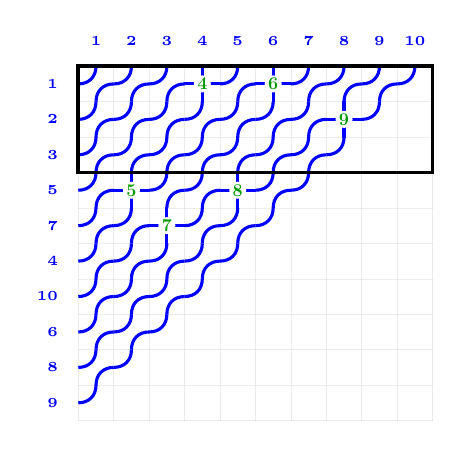
\begin{tikzpicture}[scale=0.45]
  \draw[lightgray, very thin, opacity=0.3] (10.3,0) -- (0.3,0);
  \draw[lightgray, very thin, opacity=0.3] (10.3,0) -- (10.3,10);
  \draw[lightgray, very thin, opacity=0.3] (10.3,1) -- (0.3,1);
  \draw[lightgray, very thin, opacity=0.3] (9.3,0) -- (9.3,10);
  \draw[lightgray, very thin, opacity=0.3] (10.3,2) -- (0.3,2);
  \draw[lightgray, very thin, opacity=0.3] (8.3,0) -- (8.3,10);
  \draw[lightgray, very thin, opacity=0.3] (10.3,3) -- (0.3,3);
  \draw[lightgray, very thin, opacity=0.3] (7.3,0) -- (7.3,10);
  \draw[lightgray, very thin, opacity=0.3] (10.3,4) -- (0.3,4);
  \draw[lightgray, very thin, opacity=0.3] (6.3,0) -- (6.3,10);
  \draw[lightgray, very thin, opacity=0.3] (10.3,5) -- (0.3,5);
  \draw[lightgray, very thin, opacity=0.3] (5.3,0) -- (5.3,10);
  \draw[lightgray, very thin, opacity=0.3] (10.3,6) -- (0.3,6);
  \draw[lightgray, very thin, opacity=0.3] (4.3,0) -- (4.3,10);
  \draw[lightgray, very thin, opacity=0.3] (10.3,7) -- (0.3,7);
  \draw[lightgray, very thin, opacity=0.3] (3.3,0) -- (3.3,10);
  \draw[lightgray, very thin, opacity=0.3] (10.3,8) -- (0.3,8);
  \draw[lightgray, very thin, opacity=0.3] (2.3,0) -- (2.3,10);
  \draw[lightgray, very thin, opacity=0.3] (10.3,9) -- (0.3,9);
  \draw[lightgray, very thin, opacity=0.3] (1.3,0) -- (1.3,10);
  \draw[lightgray, very thin, opacity=0.3] (10.3,10) -- (0.3,10);
  \draw[lightgray, very thin, opacity=0.3] (0.3,0) -- (0.3,10);
  \draw[blue, line width=1.125pt] (0.3,9.5) .. controls (0.6,9.5) and (0.8,9.7) .. (0.8,10);
  \draw[blue, line width=1.125pt] (0.8,9) .. controls (0.8,9.3) and (1,9.5) .. (1.3,9.5);
  \draw[blue, line width=1.125pt] (1.3,9.5) .. controls (1.6,9.5) and (1.8,9.7) .. (1.8,10);
  \draw[blue, line width=1.125pt] (1.8,9) .. controls (1.8,9.3) and (2,9.5) .. (2.3,9.5);
  \draw[blue, line width=1.125pt] (2.3,9.5) .. controls (2.6,9.5) and (2.8,9.7) .. (2.8,10);
  \draw[blue, line width=1.125pt] (2.8,9) .. controls (2.8,9.3) and (3,9.5) .. (3.3,9.5);
  \draw[blue, line width=1.125pt, line cap=round] (3.3,9.5) -- (4.3,9.5);
  \draw[blue, line width=1.125pt, line cap=round] (3.8,9) -- (3.8,10);
  \draw[blue, line width=1.125pt] (4.3,9.5) .. controls (4.6,9.5) and (4.8,9.7) .. (4.8,10);
  \draw[blue, line width=1.125pt] (4.8,9) .. controls (4.8,9.3) and (5,9.5) .. (5.3,9.5);
  \draw[blue, line width=1.125pt, line cap=round] (5.3,9.5) -- (6.3,9.5);
  \draw[blue, line width=1.125pt, line cap=round] (5.8,9) -- (5.8,10);
  \draw[blue, line width=1.125pt] (6.3,9.5) .. controls (6.6,9.5) and (6.8,9.7) .. (6.8,10);
  \draw[blue, line width=1.125pt] (6.8,9) .. controls (6.8,9.3) and (7,9.5) .. (7.3,9.5);
  \draw[blue, line width=1.125pt] (7.3,9.5) .. controls (7.6,9.5) and (7.8,9.7) .. (7.8,10);
  \draw[blue, line width=1.125pt] (7.8,9) .. controls (7.8,9.3) and (8,9.5) .. (8.3,9.5);
  \draw[blue, line width=1.125pt] (8.3,9.5) .. controls (8.6,9.5) and (8.8,9.7) .. (8.8,10);
  \draw[blue, line width=1.125pt] (8.8,9) .. controls (8.8,9.3) and (9,9.5) .. (9.3,9.5);
  \draw[blue, line width=1.125pt] (9.3,9.5) .. controls (9.6,9.5) and (9.8,9.7) .. (9.8,10);
  \draw[blue, line width=1.125pt] (0.3,8.5) .. controls (0.6,8.5) and (0.8,8.7) .. (0.8,9);
  \draw[blue, line width=1.125pt] (0.8,8) .. controls (0.8,8.3) and (1,8.5) .. (1.3,8.5);
  \draw[blue, line width=1.125pt] (1.3,8.5) .. controls (1.6,8.5) and (1.8,8.7) .. (1.8,9);
  \draw[blue, line width=1.125pt] (1.8,8) .. controls (1.8,8.3) and (2,8.5) .. (2.3,8.5);
  \draw[blue, line width=1.125pt] (2.3,8.5) .. controls (2.6,8.5) and (2.8,8.7) .. (2.8,9);
  \draw[blue, line width=1.125pt] (2.8,8) .. controls (2.8,8.3) and (3,8.5) .. (3.3,8.5);
  \draw[blue, line width=1.125pt] (3.3,8.5) .. controls (3.6,8.5) and (3.8,8.7) .. (3.8,9);
  \draw[blue, line width=1.125pt] (3.8,8) .. controls (3.8,8.3) and (4,8.5) .. (4.3,8.5);
  \draw[blue, line width=1.125pt] (4.3,8.5) .. controls (4.6,8.5) and (4.8,8.7) .. (4.8,9);
  \draw[blue, line width=1.125pt] (4.8,8) .. controls (4.8,8.3) and (5,8.5) .. (5.3,8.5);
  \draw[blue, line width=1.125pt] (5.3,8.5) .. controls (5.6,8.5) and (5.8,8.7) .. (5.8,9);
  \draw[blue, line width=1.125pt] (5.8,8) .. controls (5.8,8.3) and (6,8.5) .. (6.3,8.5);
  \draw[blue, line width=1.125pt] (6.3,8.5) .. controls (6.6,8.5) and (6.8,8.7) .. (6.8,9);
  \draw[blue, line width=1.125pt] (6.8,8) .. controls (6.8,8.3) and (7,8.5) .. (7.3,8.5);
  \draw[blue, line width=1.125pt, line cap=round] (7.3,8.5) -- (8.3,8.5);
  \draw[blue, line width=1.125pt, line cap=round] (7.8,8) -- (7.8,9);
  \draw[blue, line width=1.125pt] (8.3,8.5) .. controls (8.6,8.5) and (8.8,8.7) .. (8.8,9);
  \draw[blue, line width=1.125pt] (0.3,7.5) .. controls (0.6,7.5) and (0.8,7.7) .. (0.8,8);
  \draw[blue, line width=1.125pt] (0.8,7) .. controls (0.8,7.3) and (1,7.5) .. (1.3,7.5);
  \draw[blue, line width=1.125pt] (1.3,7.5) .. controls (1.6,7.5) and (1.8,7.7) .. (1.8,8);
  \draw[blue, line width=1.125pt] (1.8,7) .. controls (1.8,7.3) and (2,7.5) .. (2.3,7.5);
  \draw[blue, line width=1.125pt] (2.3,7.5) .. controls (2.6,7.5) and (2.8,7.7) .. (2.8,8);
  \draw[blue, line width=1.125pt] (2.8,7) .. controls (2.8,7.3) and (3,7.5) .. (3.3,7.5);
  \draw[blue, line width=1.125pt] (3.3,7.5) .. controls (3.6,7.5) and (3.8,7.7) .. (3.8,8);
  \draw[blue, line width=1.125pt] (3.8,7) .. controls (3.8,7.3) and (4,7.5) .. (4.3,7.5);
  \draw[blue, line width=1.125pt] (4.3,7.5) .. controls (4.6,7.5) and (4.8,7.7) .. (4.8,8);
  \draw[blue, line width=1.125pt] (4.8,7) .. controls (4.8,7.3) and (5,7.5) .. (5.3,7.5);
  \draw[blue, line width=1.125pt] (5.3,7.5) .. controls (5.6,7.5) and (5.8,7.7) .. (5.8,8);
  \draw[blue, line width=1.125pt] (5.8,7) .. controls (5.8,7.3) and (6,7.5) .. (6.3,7.5);
  \draw[blue, line width=1.125pt] (6.3,7.5) .. controls (6.6,7.5) and (6.8,7.7) .. (6.8,8);
  \draw[blue, line width=1.125pt] (6.8,7) .. controls (6.8,7.3) and (7,7.5) .. (7.3,7.5);
  \draw[blue, line width=1.125pt] (7.3,7.5) .. controls (7.6,7.5) and (7.8,7.7) .. (7.8,8);
  \draw[blue, line width=1.125pt] (0.3,6.5) .. controls (0.6,6.5) and (0.8,6.7) .. (0.8,7);
  \draw[blue, line width=1.125pt] (0.8,6) .. controls (0.8,6.3) and (1,6.5) .. (1.3,6.5);
  \draw[blue, line width=1.125pt, line cap=round] (1.3,6.5) -- (2.3,6.5);
  \draw[blue, line width=1.125pt, line cap=round] (1.8,6) -- (1.8,7);
  \draw[blue, line width=1.125pt] (2.3,6.5) .. controls (2.6,6.5) and (2.8,6.7) .. (2.8,7);
  \draw[blue, line width=1.125pt] (2.8,6) .. controls (2.8,6.3) and (3,6.5) .. (3.3,6.5);
  \draw[blue, line width=1.125pt] (3.3,6.5) .. controls (3.6,6.5) and (3.8,6.7) .. (3.8,7);
  \draw[blue, line width=1.125pt] (3.8,6) .. controls (3.8,6.3) and (4,6.5) .. (4.3,6.5);
  \draw[blue, line width=1.125pt, line cap=round] (4.3,6.5) -- (5.3,6.5);
  \draw[blue, line width=1.125pt, line cap=round] (4.8,6) -- (4.8,7);
  \draw[blue, line width=1.125pt] (5.3,6.5) .. controls (5.6,6.5) and (5.8,6.7) .. (5.8,7);
  \draw[blue, line width=1.125pt] (5.8,6) .. controls (5.8,6.3) and (6,6.5) .. (6.3,6.5);
  \draw[blue, line width=1.125pt] (6.3,6.5) .. controls (6.6,6.5) and (6.8,6.7) .. (6.8,7);
  \draw[blue, line width=1.125pt] (0.3,5.5) .. controls (0.6,5.5) and (0.8,5.7) .. (0.8,6);
  \draw[blue, line width=1.125pt] (0.8,5) .. controls (0.8,5.3) and (1,5.5) .. (1.3,5.5);
  \draw[blue, line width=1.125pt] (1.3,5.5) .. controls (1.6,5.5) and (1.8,5.7) .. (1.8,6);
  \draw[blue, line width=1.125pt] (1.8,5) .. controls (1.8,5.3) and (2,5.5) .. (2.3,5.5);
  \draw[blue, line width=1.125pt, line cap=round] (2.3,5.5) -- (3.3,5.5);
  \draw[blue, line width=1.125pt, line cap=round] (2.8,5) -- (2.8,6);
  \draw[blue, line width=1.125pt] (3.3,5.5) .. controls (3.6,5.5) and (3.8,5.7) .. (3.8,6);
  \draw[blue, line width=1.125pt] (3.8,5) .. controls (3.8,5.3) and (4,5.5) .. (4.3,5.5);
  \draw[blue, line width=1.125pt] (4.3,5.5) .. controls (4.6,5.5) and (4.8,5.7) .. (4.8,6);
  \draw[blue, line width=1.125pt] (4.8,5) .. controls (4.8,5.3) and (5,5.5) .. (5.3,5.5);
  \draw[blue, line width=1.125pt] (5.3,5.5) .. controls (5.6,5.5) and (5.8,5.7) .. (5.8,6);
  \draw[blue, line width=1.125pt] (0.3,4.5) .. controls (0.6,4.5) and (0.8,4.7) .. (0.8,5);
  \draw[blue, line width=1.125pt] (0.8,4) .. controls (0.8,4.3) and (1,4.5) .. (1.3,4.5);
  \draw[blue, line width=1.125pt] (1.3,4.5) .. controls (1.6,4.5) and (1.8,4.7) .. (1.8,5);
  \draw[blue, line width=1.125pt] (1.8,4) .. controls (1.8,4.3) and (2,4.5) .. (2.3,4.5);
  \draw[blue, line width=1.125pt] (2.3,4.5) .. controls (2.6,4.5) and (2.8,4.7) .. (2.8,5);
  \draw[blue, line width=1.125pt] (2.8,4) .. controls (2.8,4.3) and (3,4.5) .. (3.3,4.5);
  \draw[blue, line width=1.125pt] (3.3,4.5) .. controls (3.6,4.5) and (3.8,4.7) .. (3.8,5);
  \draw[blue, line width=1.125pt] (3.8,4) .. controls (3.8,4.3) and (4,4.5) .. (4.3,4.5);
  \draw[blue, line width=1.125pt] (4.3,4.5) .. controls (4.6,4.5) and (4.8,4.7) .. (4.8,5);
  \draw[blue, line width=1.125pt] (0.3,3.5) .. controls (0.6,3.5) and (0.8,3.7) .. (0.8,4);
  \draw[blue, line width=1.125pt] (0.8,3) .. controls (0.8,3.3) and (1,3.5) .. (1.3,3.5);
  \draw[blue, line width=1.125pt] (1.3,3.5) .. controls (1.6,3.5) and (1.8,3.7) .. (1.8,4);
  \draw[blue, line width=1.125pt] (1.8,3) .. controls (1.8,3.3) and (2,3.5) .. (2.3,3.5);
  \draw[blue, line width=1.125pt] (2.3,3.5) .. controls (2.6,3.5) and (2.8,3.7) .. (2.8,4);
  \draw[blue, line width=1.125pt] (2.8,3) .. controls (2.8,3.3) and (3,3.5) .. (3.3,3.5);
  \draw[blue, line width=1.125pt] (3.3,3.5) .. controls (3.6,3.5) and (3.8,3.7) .. (3.8,4);
  \draw[blue, line width=1.125pt] (0.3,2.5) .. controls (0.6,2.5) and (0.8,2.7) .. (0.8,3);
  \draw[blue, line width=1.125pt] (0.8,2) .. controls (0.8,2.3) and (1,2.5) .. (1.3,2.5);
  \draw[blue, line width=1.125pt] (1.3,2.5) .. controls (1.6,2.5) and (1.8,2.7) .. (1.8,3);
  \draw[blue, line width=1.125pt] (1.8,2) .. controls (1.8,2.3) and (2,2.5) .. (2.3,2.5);
  \draw[blue, line width=1.125pt] (2.3,2.5) .. controls (2.6,2.5) and (2.8,2.7) .. (2.8,3);
  \draw[blue, line width=1.125pt] (0.3,1.5) .. controls (0.6,1.5) and (0.8,1.7) .. (0.8,2);
  \draw[blue, line width=1.125pt] (0.8,1) .. controls (0.8,1.3) and (1,1.5) .. (1.3,1.5);
  \draw[blue, line width=1.125pt] (1.3,1.5) .. controls (1.6,1.5) and (1.8,1.7) .. (1.8,2);
  \draw[blue, line width=1.125pt] (0.3,0.5) .. controls (0.6,0.5) and (0.8,0.7) .. (0.8,1);
  \node[font=\tiny\bfseries, text=blue, anchor=south] at (0.8,10.3) {1};
  \node[font=\tiny\bfseries, text=blue, anchor=south] at (1.8,10.3) {2};
  \node[font=\tiny\bfseries, text=blue, anchor=south] at (2.8,10.3) {3};
  \node[font=\tiny\bfseries, text=blue, anchor=south] at (3.8,10.3) {4};
  \node[font=\tiny\bfseries, text=blue, anchor=south] at (4.8,10.3) {5};
  \node[font=\tiny\bfseries, text=blue, anchor=south] at (5.8,10.3) {6};
  \node[font=\tiny\bfseries, text=blue, anchor=south] at (6.8,10.3) {7};
  \node[font=\tiny\bfseries, text=blue, anchor=south] at (7.8,10.3) {8};
  \node[font=\tiny\bfseries, text=blue, anchor=south] at (8.8,10.3) {9};
  \node[font=\tiny\bfseries, text=blue, anchor=south] at (9.8,10.3) {10};
  \node[font=\tiny\bfseries, text=blue, anchor=east] at (0,9.5) {1};
  \node[font=\tiny\bfseries, text=blue, anchor=east] at (0,8.5) {2};
  \node[font=\tiny\bfseries, text=blue, anchor=east] at (0,7.5) {3};
  \node[font=\tiny\bfseries, text=blue, anchor=east] at (0,6.5) {5};
  \node[font=\tiny\bfseries, text=blue, anchor=east] at (0,5.5) {7};
  \node[font=\tiny\bfseries, text=blue, anchor=east] at (0,4.5) {4};
  \node[font=\tiny\bfseries, text=blue, anchor=east] at (0,3.5) {10};
  \node[font=\tiny\bfseries, text=blue, anchor=east] at (0,2.5) {6};
  \node[font=\tiny\bfseries, text=blue, anchor=east] at (0,1.5) {8};
  \node[font=\tiny\bfseries, text=blue, anchor=east] at (0,0.5) {9};
  \draw[black, line width=1.35pt] (10.3,7) rectangle (0.3,10);
  \node[font=\Large\bfseries, text=green!60!black, fill=white, inner sep=0.5pt, circle, transform shape] at (3.8,9.5) {4};
  \node[font=\Large\bfseries, text=green!60!black, fill=white, inner sep=0.5pt, circle, transform shape] at (5.8,9.5) {6};
  \node[font=\Large\bfseries, text=green!60!black, fill=white, inner sep=0.5pt, circle, transform shape] at (7.8,8.5) {9};
  \node[font=\Large\bfseries, text=green!60!black, fill=white, inner sep=0.5pt, circle, transform shape] at (1.8,6.5) {5};
  \node[font=\Large\bfseries, text=green!60!black, fill=white, inner sep=0.5pt, circle, transform shape] at (4.8,6.5) {8};
  \node[font=\Large\bfseries, text=green!60!black, fill=white, inner sep=0.5pt, circle, transform shape] at (2.8,5.5) {7};
\end{tikzpicture}
&
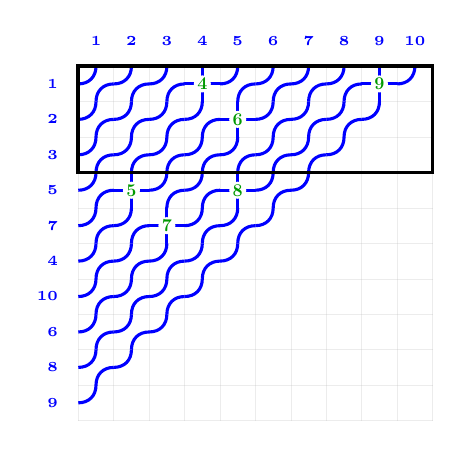
\begin{tikzpicture}[scale=0.45]
  \draw[lightgray, very thin, opacity=0.3] (10.3,0) -- (0.3,0);
  \draw[lightgray, very thin, opacity=0.3] (10.3,0) -- (10.3,10);
  \draw[lightgray, very thin, opacity=0.3] (10.3,1) -- (0.3,1);
  \draw[lightgray, very thin, opacity=0.3] (9.3,0) -- (9.3,10);
  \draw[lightgray, very thin, opacity=0.3] (10.3,2) -- (0.3,2);
  \draw[lightgray, very thin, opacity=0.3] (8.3,0) -- (8.3,10);
  \draw[lightgray, very thin, opacity=0.3] (10.3,3) -- (0.3,3);
  \draw[lightgray, very thin, opacity=0.3] (7.3,0) -- (7.3,10);
  \draw[lightgray, very thin, opacity=0.3] (10.3,4) -- (0.3,4);
  \draw[lightgray, very thin, opacity=0.3] (6.3,0) -- (6.3,10);
  \draw[lightgray, very thin, opacity=0.3] (10.3,5) -- (0.3,5);
  \draw[lightgray, very thin, opacity=0.3] (5.3,0) -- (5.3,10);
  \draw[lightgray, very thin, opacity=0.3] (10.3,6) -- (0.3,6);
  \draw[lightgray, very thin, opacity=0.3] (4.3,0) -- (4.3,10);
  \draw[lightgray, very thin, opacity=0.3] (10.3,7) -- (0.3,7);
  \draw[lightgray, very thin, opacity=0.3] (3.3,0) -- (3.3,10);
  \draw[lightgray, very thin, opacity=0.3] (10.3,8) -- (0.3,8);
  \draw[lightgray, very thin, opacity=0.3] (2.3,0) -- (2.3,10);
  \draw[lightgray, very thin, opacity=0.3] (10.3,9) -- (0.3,9);
  \draw[lightgray, very thin, opacity=0.3] (1.3,0) -- (1.3,10);
  \draw[lightgray, very thin, opacity=0.3] (10.3,10) -- (0.3,10);
  \draw[lightgray, very thin, opacity=0.3] (0.3,0) -- (0.3,10);
  \draw[blue, line width=1.125pt] (0.3,9.5) .. controls (0.6,9.5) and (0.8,9.7) .. (0.8,10);
  \draw[blue, line width=1.125pt] (0.8,9) .. controls (0.8,9.3) and (1,9.5) .. (1.3,9.5);
  \draw[blue, line width=1.125pt] (1.3,9.5) .. controls (1.6,9.5) and (1.8,9.7) .. (1.8,10);
  \draw[blue, line width=1.125pt] (1.8,9) .. controls (1.8,9.3) and (2,9.5) .. (2.3,9.5);
  \draw[blue, line width=1.125pt] (2.3,9.5) .. controls (2.6,9.5) and (2.8,9.7) .. (2.8,10);
  \draw[blue, line width=1.125pt] (2.8,9) .. controls (2.8,9.3) and (3,9.5) .. (3.3,9.5);
  \draw[blue, line width=1.125pt, line cap=round] (3.3,9.5) -- (4.3,9.5);
  \draw[blue, line width=1.125pt, line cap=round] (3.8,9) -- (3.8,10);
  \draw[blue, line width=1.125pt] (4.3,9.5) .. controls (4.6,9.5) and (4.8,9.7) .. (4.8,10);
  \draw[blue, line width=1.125pt] (4.8,9) .. controls (4.8,9.3) and (5,9.5) .. (5.3,9.5);
  \draw[blue, line width=1.125pt] (5.3,9.5) .. controls (5.6,9.5) and (5.8,9.7) .. (5.8,10);
  \draw[blue, line width=1.125pt] (5.8,9) .. controls (5.8,9.3) and (6,9.5) .. (6.3,9.5);
  \draw[blue, line width=1.125pt] (6.3,9.5) .. controls (6.6,9.5) and (6.8,9.7) .. (6.8,10);
  \draw[blue, line width=1.125pt] (6.8,9) .. controls (6.8,9.3) and (7,9.5) .. (7.3,9.5);
  \draw[blue, line width=1.125pt] (7.3,9.5) .. controls (7.6,9.5) and (7.8,9.7) .. (7.8,10);
  \draw[blue, line width=1.125pt] (7.8,9) .. controls (7.8,9.3) and (8,9.5) .. (8.3,9.5);
  \draw[blue, line width=1.125pt, line cap=round] (8.3,9.5) -- (9.3,9.5);
  \draw[blue, line width=1.125pt, line cap=round] (8.8,9) -- (8.8,10);
  \draw[blue, line width=1.125pt] (9.3,9.5) .. controls (9.6,9.5) and (9.8,9.7) .. (9.8,10);
  \draw[blue, line width=1.125pt] (0.3,8.5) .. controls (0.6,8.5) and (0.8,8.7) .. (0.8,9);
  \draw[blue, line width=1.125pt] (0.8,8) .. controls (0.8,8.3) and (1,8.5) .. (1.3,8.5);
  \draw[blue, line width=1.125pt] (1.3,8.5) .. controls (1.6,8.5) and (1.8,8.7) .. (1.8,9);
  \draw[blue, line width=1.125pt] (1.8,8) .. controls (1.8,8.3) and (2,8.5) .. (2.3,8.5);
  \draw[blue, line width=1.125pt] (2.3,8.5) .. controls (2.6,8.5) and (2.8,8.7) .. (2.8,9);
  \draw[blue, line width=1.125pt] (2.8,8) .. controls (2.8,8.3) and (3,8.5) .. (3.3,8.5);
  \draw[blue, line width=1.125pt] (3.3,8.5) .. controls (3.6,8.5) and (3.8,8.7) .. (3.8,9);
  \draw[blue, line width=1.125pt] (3.8,8) .. controls (3.8,8.3) and (4,8.5) .. (4.3,8.5);
  \draw[blue, line width=1.125pt, line cap=round] (4.3,8.5) -- (5.3,8.5);
  \draw[blue, line width=1.125pt, line cap=round] (4.8,8) -- (4.8,9);
  \draw[blue, line width=1.125pt] (5.3,8.5) .. controls (5.6,8.5) and (5.8,8.7) .. (5.8,9);
  \draw[blue, line width=1.125pt] (5.8,8) .. controls (5.8,8.3) and (6,8.5) .. (6.3,8.5);
  \draw[blue, line width=1.125pt] (6.3,8.5) .. controls (6.6,8.5) and (6.8,8.7) .. (6.8,9);
  \draw[blue, line width=1.125pt] (6.8,8) .. controls (6.8,8.3) and (7,8.5) .. (7.3,8.5);
  \draw[blue, line width=1.125pt] (7.3,8.5) .. controls (7.6,8.5) and (7.8,8.7) .. (7.8,9);
  \draw[blue, line width=1.125pt] (7.8,8) .. controls (7.8,8.3) and (8,8.5) .. (8.3,8.5);
  \draw[blue, line width=1.125pt] (8.3,8.5) .. controls (8.6,8.5) and (8.8,8.7) .. (8.8,9);
  \draw[blue, line width=1.125pt] (0.3,7.5) .. controls (0.6,7.5) and (0.8,7.7) .. (0.8,8);
  \draw[blue, line width=1.125pt] (0.8,7) .. controls (0.8,7.3) and (1,7.5) .. (1.3,7.5);
  \draw[blue, line width=1.125pt] (1.3,7.5) .. controls (1.6,7.5) and (1.8,7.7) .. (1.8,8);
  \draw[blue, line width=1.125pt] (1.8,7) .. controls (1.8,7.3) and (2,7.5) .. (2.3,7.5);
  \draw[blue, line width=1.125pt] (2.3,7.5) .. controls (2.6,7.5) and (2.8,7.7) .. (2.8,8);
  \draw[blue, line width=1.125pt] (2.8,7) .. controls (2.8,7.3) and (3,7.5) .. (3.3,7.5);
  \draw[blue, line width=1.125pt] (3.3,7.5) .. controls (3.6,7.5) and (3.8,7.7) .. (3.8,8);
  \draw[blue, line width=1.125pt] (3.8,7) .. controls (3.8,7.3) and (4,7.5) .. (4.3,7.5);
  \draw[blue, line width=1.125pt] (4.3,7.5) .. controls (4.6,7.5) and (4.8,7.7) .. (4.8,8);
  \draw[blue, line width=1.125pt] (4.8,7) .. controls (4.8,7.3) and (5,7.5) .. (5.3,7.5);
  \draw[blue, line width=1.125pt] (5.3,7.5) .. controls (5.6,7.5) and (5.8,7.7) .. (5.8,8);
  \draw[blue, line width=1.125pt] (5.8,7) .. controls (5.8,7.3) and (6,7.5) .. (6.3,7.5);
  \draw[blue, line width=1.125pt] (6.3,7.5) .. controls (6.6,7.5) and (6.8,7.7) .. (6.8,8);
  \draw[blue, line width=1.125pt] (6.8,7) .. controls (6.8,7.3) and (7,7.5) .. (7.3,7.5);
  \draw[blue, line width=1.125pt] (7.3,7.5) .. controls (7.6,7.5) and (7.8,7.7) .. (7.8,8);
  \draw[blue, line width=1.125pt] (0.3,6.5) .. controls (0.6,6.5) and (0.8,6.7) .. (0.8,7);
  \draw[blue, line width=1.125pt] (0.8,6) .. controls (0.8,6.3) and (1,6.5) .. (1.3,6.5);
  \draw[blue, line width=1.125pt, line cap=round] (1.3,6.5) -- (2.3,6.5);
  \draw[blue, line width=1.125pt, line cap=round] (1.8,6) -- (1.8,7);
  \draw[blue, line width=1.125pt] (2.3,6.5) .. controls (2.6,6.5) and (2.8,6.7) .. (2.8,7);
  \draw[blue, line width=1.125pt] (2.8,6) .. controls (2.8,6.3) and (3,6.5) .. (3.3,6.5);
  \draw[blue, line width=1.125pt] (3.3,6.5) .. controls (3.6,6.5) and (3.8,6.7) .. (3.8,7);
  \draw[blue, line width=1.125pt] (3.8,6) .. controls (3.8,6.3) and (4,6.5) .. (4.3,6.5);
  \draw[blue, line width=1.125pt, line cap=round] (4.3,6.5) -- (5.3,6.5);
  \draw[blue, line width=1.125pt, line cap=round] (4.8,6) -- (4.8,7);
  \draw[blue, line width=1.125pt] (5.3,6.5) .. controls (5.6,6.5) and (5.8,6.7) .. (5.8,7);
  \draw[blue, line width=1.125pt] (5.8,6) .. controls (5.8,6.3) and (6,6.5) .. (6.3,6.5);
  \draw[blue, line width=1.125pt] (6.3,6.5) .. controls (6.6,6.5) and (6.8,6.7) .. (6.8,7);
  \draw[blue, line width=1.125pt] (0.3,5.5) .. controls (0.6,5.5) and (0.8,5.7) .. (0.8,6);
  \draw[blue, line width=1.125pt] (0.8,5) .. controls (0.8,5.3) and (1,5.5) .. (1.3,5.5);
  \draw[blue, line width=1.125pt] (1.3,5.5) .. controls (1.6,5.5) and (1.8,5.7) .. (1.8,6);
  \draw[blue, line width=1.125pt] (1.8,5) .. controls (1.8,5.3) and (2,5.5) .. (2.3,5.5);
  \draw[blue, line width=1.125pt, line cap=round] (2.3,5.5) -- (3.3,5.5);
  \draw[blue, line width=1.125pt, line cap=round] (2.8,5) -- (2.8,6);
  \draw[blue, line width=1.125pt] (3.3,5.5) .. controls (3.6,5.5) and (3.8,5.7) .. (3.8,6);
  \draw[blue, line width=1.125pt] (3.8,5) .. controls (3.8,5.3) and (4,5.5) .. (4.3,5.5);
  \draw[blue, line width=1.125pt] (4.3,5.5) .. controls (4.6,5.5) and (4.8,5.7) .. (4.8,6);
  \draw[blue, line width=1.125pt] (4.8,5) .. controls (4.8,5.3) and (5,5.5) .. (5.3,5.5);
  \draw[blue, line width=1.125pt] (5.3,5.5) .. controls (5.6,5.5) and (5.8,5.7) .. (5.8,6);
  \draw[blue, line width=1.125pt] (0.3,4.5) .. controls (0.6,4.5) and (0.8,4.7) .. (0.8,5);
  \draw[blue, line width=1.125pt] (0.8,4) .. controls (0.8,4.3) and (1,4.5) .. (1.3,4.5);
  \draw[blue, line width=1.125pt] (1.3,4.5) .. controls (1.6,4.5) and (1.8,4.7) .. (1.8,5);
  \draw[blue, line width=1.125pt] (1.8,4) .. controls (1.8,4.3) and (2,4.5) .. (2.3,4.5);
  \draw[blue, line width=1.125pt] (2.3,4.5) .. controls (2.6,4.5) and (2.8,4.7) .. (2.8,5);
  \draw[blue, line width=1.125pt] (2.8,4) .. controls (2.8,4.3) and (3,4.5) .. (3.3,4.5);
  \draw[blue, line width=1.125pt] (3.3,4.5) .. controls (3.6,4.5) and (3.8,4.7) .. (3.8,5);
  \draw[blue, line width=1.125pt] (3.8,4) .. controls (3.8,4.3) and (4,4.5) .. (4.3,4.5);
  \draw[blue, line width=1.125pt] (4.3,4.5) .. controls (4.6,4.5) and (4.8,4.7) .. (4.8,5);
  \draw[blue, line width=1.125pt] (0.3,3.5) .. controls (0.6,3.5) and (0.8,3.7) .. (0.8,4);
  \draw[blue, line width=1.125pt] (0.8,3) .. controls (0.8,3.3) and (1,3.5) .. (1.3,3.5);
  \draw[blue, line width=1.125pt] (1.3,3.5) .. controls (1.6,3.5) and (1.8,3.7) .. (1.8,4);
  \draw[blue, line width=1.125pt] (1.8,3) .. controls (1.8,3.3) and (2,3.5) .. (2.3,3.5);
  \draw[blue, line width=1.125pt] (2.3,3.5) .. controls (2.6,3.5) and (2.8,3.7) .. (2.8,4);
  \draw[blue, line width=1.125pt] (2.8,3) .. controls (2.8,3.3) and (3,3.5) .. (3.3,3.5);
  \draw[blue, line width=1.125pt] (3.3,3.5) .. controls (3.6,3.5) and (3.8,3.7) .. (3.8,4);
  \draw[blue, line width=1.125pt] (0.3,2.5) .. controls (0.6,2.5) and (0.8,2.7) .. (0.8,3);
  \draw[blue, line width=1.125pt] (0.8,2) .. controls (0.8,2.3) and (1,2.5) .. (1.3,2.5);
  \draw[blue, line width=1.125pt] (1.3,2.5) .. controls (1.6,2.5) and (1.8,2.7) .. (1.8,3);
  \draw[blue, line width=1.125pt] (1.8,2) .. controls (1.8,2.3) and (2,2.5) .. (2.3,2.5);
  \draw[blue, line width=1.125pt] (2.3,2.5) .. controls (2.6,2.5) and (2.8,2.7) .. (2.8,3);
  \draw[blue, line width=1.125pt] (0.3,1.5) .. controls (0.6,1.5) and (0.8,1.7) .. (0.8,2);
  \draw[blue, line width=1.125pt] (0.8,1) .. controls (0.8,1.3) and (1,1.5) .. (1.3,1.5);
  \draw[blue, line width=1.125pt] (1.3,1.5) .. controls (1.6,1.5) and (1.8,1.7) .. (1.8,2);
  \draw[blue, line width=1.125pt] (0.3,0.5) .. controls (0.6,0.5) and (0.8,0.7) .. (0.8,1);
  \node[font=\tiny\bfseries, text=blue, anchor=south] at (0.8,10.3) {1};
  \node[font=\tiny\bfseries, text=blue, anchor=south] at (1.8,10.3) {2};
  \node[font=\tiny\bfseries, text=blue, anchor=south] at (2.8,10.3) {3};
  \node[font=\tiny\bfseries, text=blue, anchor=south] at (3.8,10.3) {4};
  \node[font=\tiny\bfseries, text=blue, anchor=south] at (4.8,10.3) {5};
  \node[font=\tiny\bfseries, text=blue, anchor=south] at (5.8,10.3) {6};
  \node[font=\tiny\bfseries, text=blue, anchor=south] at (6.8,10.3) {7};
  \node[font=\tiny\bfseries, text=blue, anchor=south] at (7.8,10.3) {8};
  \node[font=\tiny\bfseries, text=blue, anchor=south] at (8.8,10.3) {9};
  \node[font=\tiny\bfseries, text=blue, anchor=south] at (9.8,10.3) {10};
  \node[font=\tiny\bfseries, text=blue, anchor=east] at (0,9.5) {1};
  \node[font=\tiny\bfseries, text=blue, anchor=east] at (0,8.5) {2};
  \node[font=\tiny\bfseries, text=blue, anchor=east] at (0,7.5) {3};
  \node[font=\tiny\bfseries, text=blue, anchor=east] at (0,6.5) {5};
  \node[font=\tiny\bfseries, text=blue, anchor=east] at (0,5.5) {7};
  \node[font=\tiny\bfseries, text=blue, anchor=east] at (0,4.5) {4};
  \node[font=\tiny\bfseries, text=blue, anchor=east] at (0,3.5) {10};
  \node[font=\tiny\bfseries, text=blue, anchor=east] at (0,2.5) {6};
  \node[font=\tiny\bfseries, text=blue, anchor=east] at (0,1.5) {8};
  \node[font=\tiny\bfseries, text=blue, anchor=east] at (0,0.5) {9};
  \draw[black, line width=1.35pt] (10.3,7) rectangle (0.3,10);
  \node[font=\Large\bfseries, text=green!60!black, fill=white, inner sep=0.5pt, circle, transform shape] at (3.8,9.5) {4};
  \node[font=\Large\bfseries, text=green!60!black, fill=white, inner sep=0.5pt, circle, transform shape] at (8.8,9.5) {9};
  \node[font=\Large\bfseries, text=green!60!black, fill=white, inner sep=0.5pt, circle, transform shape] at (4.8,8.5) {6};
  \node[font=\Large\bfseries, text=green!60!black, fill=white, inner sep=0.5pt, circle, transform shape] at (1.8,6.5) {5};
  \node[font=\Large\bfseries, text=green!60!black, fill=white, inner sep=0.5pt, circle, transform shape] at (4.8,6.5) {8};
  \node[font=\Large\bfseries, text=green!60!black, fill=white, inner sep=0.5pt, circle, transform shape] at (2.8,5.5) {7};
\end{tikzpicture}
\end{tabular}
\caption{The two $7$-row RC graphs $R_1$ (left) and $R_2$ (right) in $\mathrm{Dem}_c$ satisfying $\clp^3(R_i)\in\mathrm{Dem}_a$ and $\trm^3(R_i)\in\mathrm{Dem}_b$. The outlined box marks the top $3$ rows (the clip region).}
\label{fig:LRkey_example}
\end{figure}

Both graphs have permutation $w_c=(1,2,3,5,7,4,10,6,8,9)$. They differ only in their first two rows: $R_1$ has row data $[(6,4),(9,),()]$ in the top three rows, while $R_2$ has $[(9,4),(6,),()]$. Applying $\clp^3$ (retaining only the top $3$ rows and re-indexing) to each yields the same $3$-row graph with extremal weight $a=(0,1,2)$:
$$\clp^3(R_1)=\clp^3(R_2)=
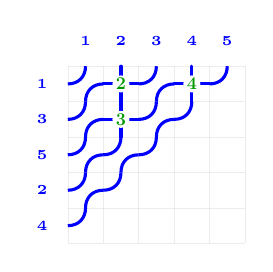
\begin{tikzpicture}[scale=0.45, baseline=(current bounding box.center)]
  \draw[lightgray, very thin, opacity=0.3] (5.3,0) -- (0.3,0);
  \draw[lightgray, very thin, opacity=0.3] (5.3,0) -- (5.3,5);
  \draw[lightgray, very thin, opacity=0.3] (5.3,1) -- (0.3,1);
  \draw[lightgray, very thin, opacity=0.3] (4.3,0) -- (4.3,5);
  \draw[lightgray, very thin, opacity=0.3] (5.3,2) -- (0.3,2);
  \draw[lightgray, very thin, opacity=0.3] (3.3,0) -- (3.3,5);
  \draw[lightgray, very thin, opacity=0.3] (5.3,3) -- (0.3,3);
  \draw[lightgray, very thin, opacity=0.3] (2.3,0) -- (2.3,5);
  \draw[lightgray, very thin, opacity=0.3] (5.3,4) -- (0.3,4);
  \draw[lightgray, very thin, opacity=0.3] (1.3,0) -- (1.3,5);
  \draw[lightgray, very thin, opacity=0.3] (5.3,5) -- (0.3,5);
  \draw[lightgray, very thin, opacity=0.3] (0.3,0) -- (0.3,5);
  \draw[blue, line width=1.125pt] (0.3,4.5) .. controls (0.6,4.5) and (0.8,4.7) .. (0.8,5);
  \draw[blue, line width=1.125pt] (0.8,4) .. controls (0.8,4.3) and (1,4.5) .. (1.3,4.5);
  \draw[blue, line width=1.125pt, line cap=round] (1.3,4.5) -- (2.3,4.5);
  \draw[blue, line width=1.125pt, line cap=round] (1.8,4) -- (1.8,5);
  \draw[blue, line width=1.125pt] (2.3,4.5) .. controls (2.6,4.5) and (2.8,4.7) .. (2.8,5);
  \draw[blue, line width=1.125pt] (2.8,4) .. controls (2.8,4.3) and (3,4.5) .. (3.3,4.5);
  \draw[blue, line width=1.125pt, line cap=round] (3.3,4.5) -- (4.3,4.5);
  \draw[blue, line width=1.125pt, line cap=round] (3.8,4) -- (3.8,5);
  \draw[blue, line width=1.125pt] (4.3,4.5) .. controls (4.6,4.5) and (4.8,4.7) .. (4.8,5);
  \draw[blue, line width=1.125pt] (0.3,3.5) .. controls (0.6,3.5) and (0.8,3.7) .. (0.8,4);
  \draw[blue, line width=1.125pt] (0.8,3) .. controls (0.8,3.3) and (1,3.5) .. (1.3,3.5);
  \draw[blue, line width=1.125pt, line cap=round] (1.3,3.5) -- (2.3,3.5);
  \draw[blue, line width=1.125pt, line cap=round] (1.8,3) -- (1.8,4);
  \draw[blue, line width=1.125pt] (2.3,3.5) .. controls (2.6,3.5) and (2.8,3.7) .. (2.8,4);
  \draw[blue, line width=1.125pt] (2.8,3) .. controls (2.8,3.3) and (3,3.5) .. (3.3,3.5);
  \draw[blue, line width=1.125pt] (3.3,3.5) .. controls (3.6,3.5) and (3.8,3.7) .. (3.8,4);
  \draw[blue, line width=1.125pt] (0.3,2.5) .. controls (0.6,2.5) and (0.8,2.7) .. (0.8,3);
  \draw[blue, line width=1.125pt] (0.8,2) .. controls (0.8,2.3) and (1,2.5) .. (1.3,2.5);
  \draw[blue, line width=1.125pt] (1.3,2.5) .. controls (1.6,2.5) and (1.8,2.7) .. (1.8,3);
  \draw[blue, line width=1.125pt] (1.8,2) .. controls (1.8,2.3) and (2,2.5) .. (2.3,2.5);
  \draw[blue, line width=1.125pt] (2.3,2.5) .. controls (2.6,2.5) and (2.8,2.7) .. (2.8,3);
  \draw[blue, line width=1.125pt] (0.3,1.5) .. controls (0.6,1.5) and (0.8,1.7) .. (0.8,2);
  \draw[blue, line width=1.125pt] (0.8,1) .. controls (0.8,1.3) and (1,1.5) .. (1.3,1.5);
  \draw[blue, line width=1.125pt] (1.3,1.5) .. controls (1.6,1.5) and (1.8,1.7) .. (1.8,2);
  \draw[blue, line width=1.125pt] (0.3,0.5) .. controls (0.6,0.5) and (0.8,0.7) .. (0.8,1);
  \node[font=\tiny\bfseries, text=blue, anchor=south] at (0.8,5.3) {1};
  \node[font=\tiny\bfseries, text=blue, anchor=south] at (1.8,5.3) {2};
  \node[font=\tiny\bfseries, text=blue, anchor=south] at (2.8,5.3) {3};
  \node[font=\tiny\bfseries, text=blue, anchor=south] at (3.8,5.3) {4};
  \node[font=\tiny\bfseries, text=blue, anchor=south] at (4.8,5.3) {5};
  \node[font=\tiny\bfseries, text=blue, anchor=east] at (0,4.5) {1};
  \node[font=\tiny\bfseries, text=blue, anchor=east] at (0,3.5) {3};
  \node[font=\tiny\bfseries, text=blue, anchor=east] at (0,2.5) {5};
  \node[font=\tiny\bfseries, text=blue, anchor=east] at (0,1.5) {2};
  \node[font=\tiny\bfseries, text=blue, anchor=east] at (0,0.5) {4};
  \node[font=\Large\bfseries, text=green!60!black, fill=white, inner sep=0.5pt, circle, transform shape] at (1.8,4.5) {2};
  \node[font=\Large\bfseries, text=green!60!black, fill=white, inner sep=0.5pt, circle, transform shape] at (3.8,4.5) {4};
  \node[font=\Large\bfseries, text=green!60!black, fill=white, inner sep=0.5pt, circle, transform shape] at (1.8,3.5) {3};
\end{tikzpicture}
$$
Applying $\trm^3$ (keeping the bottom $4$ rows) gives the same $4$-row graph with extremal weight $b=(0,1,0,2)$:
$$\trm^3(R_1)=\trm^3(R_2)=
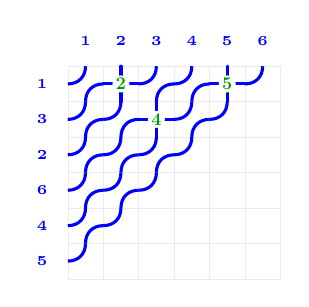
\begin{tikzpicture}[scale=0.45, baseline=(current bounding box.center)]
  \draw[lightgray, very thin, opacity=0.3] (6.3,0) -- (0.3,0);
  \draw[lightgray, very thin, opacity=0.3] (6.3,0) -- (6.3,6);
  \draw[lightgray, very thin, opacity=0.3] (6.3,1) -- (0.3,1);
  \draw[lightgray, very thin, opacity=0.3] (5.3,0) -- (5.3,6);
  \draw[lightgray, very thin, opacity=0.3] (6.3,2) -- (0.3,2);
  \draw[lightgray, very thin, opacity=0.3] (4.3,0) -- (4.3,6);
  \draw[lightgray, very thin, opacity=0.3] (6.3,3) -- (0.3,3);
  \draw[lightgray, very thin, opacity=0.3] (3.3,0) -- (3.3,6);
  \draw[lightgray, very thin, opacity=0.3] (6.3,4) -- (0.3,4);
  \draw[lightgray, very thin, opacity=0.3] (2.3,0) -- (2.3,6);
  \draw[lightgray, very thin, opacity=0.3] (6.3,5) -- (0.3,5);
  \draw[lightgray, very thin, opacity=0.3] (1.3,0) -- (1.3,6);
  \draw[lightgray, very thin, opacity=0.3] (6.3,6) -- (0.3,6);
  \draw[lightgray, very thin, opacity=0.3] (0.3,0) -- (0.3,6);
  \draw[blue, line width=1.125pt] (0.3,5.5) .. controls (0.6,5.5) and (0.8,5.7) .. (0.8,6);
  \draw[blue, line width=1.125pt] (0.8,5) .. controls (0.8,5.3) and (1,5.5) .. (1.3,5.5);
  \draw[blue, line width=1.125pt, line cap=round] (1.3,5.5) -- (2.3,5.5);
  \draw[blue, line width=1.125pt, line cap=round] (1.8,5) -- (1.8,6);
  \draw[blue, line width=1.125pt] (2.3,5.5) .. controls (2.6,5.5) and (2.8,5.7) .. (2.8,6);
  \draw[blue, line width=1.125pt] (2.8,5) .. controls (2.8,5.3) and (3,5.5) .. (3.3,5.5);
  \draw[blue, line width=1.125pt] (3.3,5.5) .. controls (3.6,5.5) and (3.8,5.7) .. (3.8,6);
  \draw[blue, line width=1.125pt] (3.8,5) .. controls (3.8,5.3) and (4,5.5) .. (4.3,5.5);
  \draw[blue, line width=1.125pt, line cap=round] (4.3,5.5) -- (5.3,5.5);
  \draw[blue, line width=1.125pt, line cap=round] (4.8,5) -- (4.8,6);
  \draw[blue, line width=1.125pt] (5.3,5.5) .. controls (5.6,5.5) and (5.8,5.7) .. (5.8,6);
  \draw[blue, line width=1.125pt] (0.3,4.5) .. controls (0.6,4.5) and (0.8,4.7) .. (0.8,5);
  \draw[blue, line width=1.125pt] (0.8,4) .. controls (0.8,4.3) and (1,4.5) .. (1.3,4.5);
  \draw[blue, line width=1.125pt] (1.3,4.5) .. controls (1.6,4.5) and (1.8,4.7) .. (1.8,5);
  \draw[blue, line width=1.125pt] (1.8,4) .. controls (1.8,4.3) and (2,4.5) .. (2.3,4.5);
  \draw[blue, line width=1.125pt, line cap=round] (2.3,4.5) -- (3.3,4.5);
  \draw[blue, line width=1.125pt, line cap=round] (2.8,4) -- (2.8,5);
  \draw[blue, line width=1.125pt] (3.3,4.5) .. controls (3.6,4.5) and (3.8,4.7) .. (3.8,5);
  \draw[blue, line width=1.125pt] (3.8,4) .. controls (3.8,4.3) and (4,4.5) .. (4.3,4.5);
  \draw[blue, line width=1.125pt] (4.3,4.5) .. controls (4.6,4.5) and (4.8,4.7) .. (4.8,5);
  \draw[blue, line width=1.125pt] (0.3,3.5) .. controls (0.6,3.5) and (0.8,3.7) .. (0.8,4);
  \draw[blue, line width=1.125pt] (0.8,3) .. controls (0.8,3.3) and (1,3.5) .. (1.3,3.5);
  \draw[blue, line width=1.125pt] (1.3,3.5) .. controls (1.6,3.5) and (1.8,3.7) .. (1.8,4);
  \draw[blue, line width=1.125pt] (1.8,3) .. controls (1.8,3.3) and (2,3.5) .. (2.3,3.5);
  \draw[blue, line width=1.125pt] (2.3,3.5) .. controls (2.6,3.5) and (2.8,3.7) .. (2.8,4);
  \draw[blue, line width=1.125pt] (2.8,3) .. controls (2.8,3.3) and (3,3.5) .. (3.3,3.5);
  \draw[blue, line width=1.125pt] (3.3,3.5) .. controls (3.6,3.5) and (3.8,3.7) .. (3.8,4);
  \draw[blue, line width=1.125pt] (0.3,2.5) .. controls (0.6,2.5) and (0.8,2.7) .. (0.8,3);
  \draw[blue, line width=1.125pt] (0.8,2) .. controls (0.8,2.3) and (1,2.5) .. (1.3,2.5);
  \draw[blue, line width=1.125pt] (1.3,2.5) .. controls (1.6,2.5) and (1.8,2.7) .. (1.8,3);
  \draw[blue, line width=1.125pt] (1.8,2) .. controls (1.8,2.3) and (2,2.5) .. (2.3,2.5);
  \draw[blue, line width=1.125pt] (2.3,2.5) .. controls (2.6,2.5) and (2.8,2.7) .. (2.8,3);
  \draw[blue, line width=1.125pt] (0.3,1.5) .. controls (0.6,1.5) and (0.8,1.7) .. (0.8,2);
  \draw[blue, line width=1.125pt] (0.8,1) .. controls (0.8,1.3) and (1,1.5) .. (1.3,1.5);
  \draw[blue, line width=1.125pt] (1.3,1.5) .. controls (1.6,1.5) and (1.8,1.7) .. (1.8,2);
  \draw[blue, line width=1.125pt] (0.3,0.5) .. controls (0.6,0.5) and (0.8,0.7) .. (0.8,1);
  \node[font=\tiny\bfseries, text=blue, anchor=south] at (0.8,6.3) {1};
  \node[font=\tiny\bfseries, text=blue, anchor=south] at (1.8,6.3) {2};
  \node[font=\tiny\bfseries, text=blue, anchor=south] at (2.8,6.3) {3};
  \node[font=\tiny\bfseries, text=blue, anchor=south] at (3.8,6.3) {4};
  \node[font=\tiny\bfseries, text=blue, anchor=south] at (4.8,6.3) {5};
  \node[font=\tiny\bfseries, text=blue, anchor=south] at (5.8,6.3) {6};
  \node[font=\tiny\bfseries, text=blue, anchor=east] at (0,5.5) {1};
  \node[font=\tiny\bfseries, text=blue, anchor=east] at (0,4.5) {3};
  \node[font=\tiny\bfseries, text=blue, anchor=east] at (0,3.5) {2};
  \node[font=\tiny\bfseries, text=blue, anchor=east] at (0,2.5) {6};
  \node[font=\tiny\bfseries, text=blue, anchor=east] at (0,1.5) {4};
  \node[font=\tiny\bfseries, text=blue, anchor=east] at (0,0.5) {5};
  \node[font=\Large\bfseries, text=green!60!black, fill=white, inner sep=0.5pt, circle, transform shape] at (1.8,5.5) {2};
  \node[font=\Large\bfseries, text=green!60!black, fill=white, inner sep=0.5pt, circle, transform shape] at (4.8,5.5) {5};
  \node[font=\Large\bfseries, text=green!60!black, fill=white, inner sep=0.5pt, circle, transform shape] at (2.8,4.5) {4};
\end{tikzpicture}
$$

Since there are exactly $2$ such RC graphs, Theorem~\ref{theorem:LRkey} gives $k_{a,b}^c = 2$.
\end{example}



\section{The ring of forest classes of RC graphs}\label{section:forest}

The \emph{forest polynomials} $\forest_a$ were introduced by Nadeau and Tewari in \cite{nadeau2024forest} and are closely related to Schubert polynomials. They can be defined by reduced words and compatible sequences, but the invariant preserved by these words is distinct from the permutation. Given a reduced word/compatible sequence pair $(\mathbf{r},\mathbf{s})$, there is an insertion algorithm that produces a corresponding invariant $\finv(\mathbf{r},\mathbf{s})$ that represents an equivalence relation on the words, where the compatible sequence can vary arbitrarily. We therefore shorten the notation to $\finv(\mathbf{r})$. The equivalence classes consist of words that are all for the same permutation, so that if we define
$$R\equiv_{\forest} R'$$
to mean that $\finv(\mathrm{word}(R)) = \finv(\mathrm{word}(R'))$, then the forest polynomials partition the set of RC graphs for the given permutation. The forest polynomials are indexed in the original work by ``indexed forests,'' hence the name. These correspond bijectively to weak compositions, so we can define a weak composition $\fcode(R)$ by associating an indexed forest to this equivalence class as in the article. Define $\mathcal{C}_\forest(a)$ for a composition $a$ to be the set of equivalence classes of RC graphs under this relation such that $\fcode(R)=a$.


\subsection{Indexed forests, forest invariant}

\begin{definition}[Indexed forests and codes]
  An \emph{indexed forest} $F$ is a pair $(S, T_\bullet)$ where $S$ is a set of positive integers, called the \emph{support} of $F$. Writing
  $$S=I_1\cup I_2\cup \cdots \cup I_k$$
  where $I_1,I_2,\ldots, I_k$ are the maximal intervals contained in $S$, we have $T_\bullet$ as a sequence of binary trees $T_1,T_2,\ldots, T_k$ where $T_j$ has $|I_j|$ internal nodes for each $j$. The internal nodes of $F$ are denoted by $\mathrm{IN}(F)$. For $v\in \mathrm{IN}(F)$, we denote by $\mathrm{left}(v)$ and $\mathrm{right}(v)$ the left and right children of $v$ respectively, which may not be in $\mathrm{IN}(F)$ if they are leaves, or may be empty.
  
  There is a natural labeling $\lambda_F:\mathrm{IN}(F)\to S$ sending each internal node, say $v\in T_j$, to the unique element of $I_j$ that is at the same index as $v\in T_j$ in the inorder traversal of $T_j$.
  
  The function $\rho_F:\mathrm{IN}(F)\to S$ is defined for an internal node $v\in T_j$ by 
  $$\rho_F(v) = \begin{cases}
  \lambda_F(v)&\mbox{ if }\mathrm{left}(v)\notin\mathrm{IN}(F)\\
  \lambda_F(\mathrm{left}(v))&\mbox{ if }\mathrm{left}(v)\in\mathrm{IN}(F).
  \end{cases}$$
  For each indexed forest $F$, we assign a weak composition $\code(F)$ by
  $$\code_j(F)=\#\{v\in \mathrm{IN}(F): \rho_F(v)=j\}$$
  Then the \emph{forest polynomial} $\forest_F(x)$ is defined by
  $$\forest_F(x) = \sum_{\tau}\prod_{v\in\mathrm{IN}(F)}x_{\tau(v)}$$
  where the sum is over all functions $\tau:\mathrm{IN}(F)\to \mathbb{Z}_{>0}$ such that $\tau(v)\leq \rho_F(v)$ for all $v\in \mathrm{IN}(F)$, $\tau(v)\leq\tau(\mathrm{left}(v))$ for all $v\in \mathrm{IN}(F)$ such that $\mathrm{left}(v)\in \mathrm{IN}(F)$, and $\tau(v)<\tau(\mathrm{right}(v))$ for all $v\in \mathrm{IN}(F)$ such that $\mathrm{right}(v)\in \mathrm{IN}(F)$.

  It is easiest for our purposes to index forest polynomials by weak compositions rather than indexed forests, so we define $\forest_a(x) = \forest_F(x)$ where $F$ is the unique indexed forest such that $\code(F) = a$.
\end{definition}

\begin{definition}[Injective words, forest invariant]
In \cite{nadeau2024ppartitions}, an alphabet $\overline{\mathbb{Z}}$ is defined as the set of pairs of integers $(i,j)$ in lexicographical order, written with the notation $i^{[j]}$. They define $\mathrm{val}(i^{[j]})=i$. An \emph{injective word} is a word $w=w_1w_2\cdots w_k$ such that $w_i\neq w_j$ for all $i\neq j$. An \emph{LBS (local binary search)  labeling} of an indexed forest $F$ is an injective function $\rho:\mathrm{IN}(F)\to \overline{\mathbb{Z}}$ such that
\begin{enumerate}
\item $\rho(\mathrm{left}(v))<\rho(v)$ for all $v\in \mathrm{IN}(F)$ such that $\mathrm{left}(v)\in \mathrm{IN}(F)$.
\item $\rho(v)<\rho(\mathrm{right}(v))$ for all $v\in \mathrm{IN}(F)$ such that $\mathrm{right}(v)\in \mathrm{IN}(F)$.
\item For all $v\in\mathrm{IN}(F)$, $\mathrm{val}(\rho(v)) = \lambda_F(u)$ for some $u\in\mathrm{IN}(F)$.
\end{enumerate}

Following \cite{nadeau2024forest}, given any injective word $w = w_1\cdots w_m$ in $\overline{\mathbb{Z}}$, we associate to it inductively an indexed forest $F(w)$, an LBS labeling $P(w)$ of $F(w)$, and an injective ``time-stamp'' labeling $Q(w):\mathrm{IN}(F(w))\to\{1,\ldots,m\}$ as follows. If $m=0$, then $F(w)$ is the empty forest. Otherwise write $w = w'a$ with $w' = w_1\cdots w_{m-1}$, and assume $F' := F(w')$, $P' := P(w')$, and $Q' := Q(w')$ have already been constructed; let $S'$ be the support of $F'$, and let $S' = I_1\cup\cdots\cup I_k$ be its decomposition into maximal intervals (listed left to right). For each $j$, denote by $u_j$ the root of the tree of $F'$ supported on $I_j$, and set $a_j := P'(u_j)$. We obtain $F(w)$ by adjoining a new internal node $u$ to $F'$, with attachments determined by $i := \mathrm{val}(a)$:
\begin{itemize}
\item If $i\notin S'$, then $u$ is the root of a new tree, with left child $u_j$ when $i-1\in I_j$ (otherwise no left child), and right child $u_j$ when $i+1\in I_j$ (otherwise no right child).
\item If $i\in I_j$, then we compare $a$ with $a_j$ in the order on $\overline{\mathbb{Z}}$:
\begin{itemize}
\item if $a>a_j$, then $u_j$ becomes the left child of $u$; additionally, if $\max(I_j)+2\in S'$ (necessarily $\max(I_j)+2 = \min(I_{j+1})$), then $u_{j+1}$ becomes the right child of $u$;
\item if $a<a_j$, then $u_j$ becomes the right child of $u$; additionally, if $\min(I_j)-2\in S'$ (necessarily $\min(I_j)-2=\max(I_{j-1})$), then $u_{j-1}$ becomes the left child of $u$.
\end{itemize}
\end{itemize}
The remaining roots of $F'$ become roots of $F(w)$ unchanged. We then extend $P'$ to $P(w)$ by setting $P(w)(u) := a$, and extend $Q'$ to $Q(w)$ by setting $Q(w)(u) := m$. The pair $(P(w), Q(w))$ is the \emph{$\Omega$-insertion} of $w$.
\end{definition}

The importance of this algorithm is

\begin{theorem}[{\cite[Theorem~5.1]{nadeau2024forest}}]
The correspondence $w\mapsto (P(w), Q(w))$ is a bijection between the following two sets:
\begin{enumerate}
\item Injective words $w$ with letters in $\overline{\mathbb{Z}}$, and
\item Pairs $(P, Q)$ such that $P \in \mathrm{LBS}(F)$ and $Q \in \mathrm{Dec}(F)$ for a common indexed forest $F$.
\end{enumerate}
\end{theorem}


\begin{definition}[Injectification, $\equiv_\forest$]
  For a word $\mathbf{r}$ in the alphabet $\mathbb{Z}$, we may canonically turn $\mathbf{r}$ into an injective word in the alphabet $\overline{\mathbb{Z}}$ by assigning superscripts consecutively starting at $1$ to break ties between equal letters.

Let $\mathbf{r}_1$ and $\mathbf{r}_2$ be reduced words. Then we say that $\mathbf{r}_1\equiv_\forest\mathbf{r}_2$ if $P(\overline{\mathbf{r}_1}) = P(\overline{\mathbf{r}_2})$. Naturally, we may apply this to RC graphs as well: for RC graphs $R_1$ and $R_2$, we say that $R_1\equiv_\forest R_2$ if $\overline{\mathrm{word}(R_1)}\equiv_\forest \overline{\mathrm{word}(R_2)}$. For a permutation $w$, we denote by $\mathcal{C}_\forest(w)$ the set of equivalence classes of reduced words for $w$ under $\equiv_\forest$.
\end{definition}

\begin{theorem}[{\cite[Theorem~1.4]{nadeau2024forest}}] \label{theorem:forestforest}
  Let $w\in S_\infty$. Then we have

  $$\sch_w(x) = \sum_{C\in \mathcal{C}_\forest(w)} \forest_{\code_\forest(C)}(x)$$
\end{theorem}


\subsection{The dual forest basis and the ring of forest classes of RC graphs}

\begin{definition}[The dual forest basis]
  For a weak composition $a$ of length $n$, define $\forest_a^*\in \dcoma_n$ to be the unique element such that $\langle \forest_a^*, \forest_b\rangle = \delta_{a,b}$ for all weak compositions $b$.
\end{definition}

We record the result that the coefficients of $\forest^*_c$ in the monomial-dual basis are exactly the forest expansion coefficients of monomials computed by Nadeau, Spink, and Tewari, and that under the Borel-type isomorphism $H^\bullet(\mathrm{QFl}_n)\cong \mathbb{Z}[x_1,\ldots,x_n]/\mathrm{QSym}_n^+$ of \cite{bergeron2025qsymflag} the same integers compute the cap product against the geometric homology basis $\{[X(F)]\}$ of $H_\bullet(\mathrm{QFl}_n)$.

\begin{proposition}\label{proposition:forestdualcoefficients}
Let $a$ be a weak composition of length $n$, and let $F_a$ denote the corresponding indexed forest. Let $\{e_{\mathbf{b}}\}_{\mathbf{b}\in \mathbb{Z}_{\geq 0}^n}$ denote the basis of $\dcoma_n$ dual to the monomial basis $\{x^{\mathbf{b}}\}$ of $\coma_n$. Then
$$\forest_a^* \;=\; \sum_{\mathbf{b}\in \mathbb{Z}_{\geq 0}^n} \epsilon_{F_a}(\mathbf{b})\,e_{\mathbf{b}}\quad\in\;\dcoma_n,$$
where $\epsilon_{F_a}(\mathbf{b})\in\{-1,0,+1\}$ is the path sign of \cite[Proposition~10.15]{nadeau2024quasisymmetric}.

The same integers admit two further interpretations:
\begin{enumerate}
\item (Volume polynomial / Postnikov--Stanley-style dual.) The volume polynomial $V_{F_a}(\boldsymbol\lambda)\in\mathbb{Q}[\lambda_1,\ldots,\lambda_n]$ of \cite[Section~10.5]{nadeau2024quasisymmetric}, which is dual to $\forest_{F_a}$ under the divided-power $D$-pairing of \emph{loc.~cit.}, expands as
$$V_{F_a}(\boldsymbol\lambda) \;=\; \sum_{\mathbf{b}\in\mathbb{Z}_{\geq 0}^n} \epsilon_{F_a}(\mathbf{b})\,\frac{\boldsymbol\lambda^{\mathbf{b}}}{\mathbf{b}!}\qquad\bigl(\text{\cite[Proposition~10.14]{nadeau2024quasisymmetric}}\bigr).$$
Up to the divided-power normalization, $V_{F_a}(\boldsymbol\lambda)$ and $\forest_a^*$ are the same linear functional on $\coma_n$, in exact analogy with the relationship between the Postnikov--Stanley dual Schubert polynomials \cite{postnikov2009chains} and our $\dsch_u^n$ noted in the introduction.

\item (Geometric Kronecker dual on $\mathrm{QFl}_n$.) Under the Borel isomorphism $\pi_n:\coma_n\twoheadrightarrow \coma_n/\mathrm{QSym}_n^+\cdot\coma_n \cong H^\bullet(\mathrm{QFl}_n)$ of \cite[Theorem~A and Corollary~12.5]{bergeron2025qsymflag}, the dual functional $\forest_a^*$ kills the kernel ideal and descends to the Kronecker dual of $[\forest_{F_a}]\in H^\bullet(\mathrm{QFl}_n)$ paired against the homology basis $\{[X(F)]:F\in\mathsf{Forest}_n\}$ of \cite[Corollary~11.6]{bergeron2025qsymflag}. Concretely, for $F_a\in\mathsf{Forest}_n$,
$$\forest_a^*\;=\;\pi_n^*\bigl([X(F_a)]\bigr) \quad\text{in}\quad \dcoma_n,$$
and equivalently
$$\int_{X(F_a)}\!\overline{x^{\mathbf{b}}} \;=\; \epsilon_{F_a}(\mathbf{b})\quad \text{in } H^\bullet(\mathrm{QFl}_n)$$
for all $\mathbf{b}\in\mathbb{Z}_{\geq 0}^n$, where $\overline{x^{\mathbf{b}}}=\pi_n(x^{\mathbf{b}})$. For $a$ with $F_a\not\in\mathsf{Forest}_n$ both sides vanish: $\forest_{F_a}\in \mathrm{QSym}_n^+\cdot\coma_n$ by \cite[Theorem~9.7]{nadeau2024quasisymmetric}, so $\forest_a^*$ vanishes on this submodule.
\end{enumerate}
\end{proposition}

\begin{proof}
The first identity is immediate: applying $\forest_a^*$ to the forest expansion of monomials $x^{\mathbf{b}}=\sum_G \epsilon_G(\mathbf{b})\,\forest_G$ \cite[Proposition~10.15]{nadeau2024quasisymmetric} gives $\langle \forest_a^*, x^{\mathbf{b}}\rangle = \sum_G \epsilon_G(\mathbf{b})\langle \forest_a^*,\forest_G\rangle = \epsilon_{F_a}(\mathbf{b})$ by the defining duality $\langle \forest_a^*,\forest_b\rangle=\delta_{a,b}$.

Item~(1) is then a direct comparison of \cite[Proposition~10.14]{nadeau2024quasisymmetric} with the displayed expansion.

For item~(2), the splitting $\coma_n = \bigoplus_{F_a\in\mathsf{Forest}_n}\mathbb{Z}\forest_a \oplus \mathrm{QSym}_n^+\cdot\coma_n$ \cite[Theorem~9.7]{nadeau2024quasisymmetric} forces $\forest_a^*$ to annihilate the kernel of $\pi_n$ when $F_a\in\mathsf{Forest}_n$, hence to factor through $\pi_n$. The induced functional pairs with $[\forest_b]$ to $\delta_{a,b}$, which is precisely the defining property of $[X(F_a)]$ \cite[Theorem~12.12]{bergeron2025qsymflag}, so $\forest_a^*=\pi_n^*([X(F_a)])$. The second equality of item~(2) is then the previous display read modulo $\mathrm{QSym}_n^+\cdot\coma_n$.
\end{proof}

In particular, the algebraic dual basis $\{\forest_a^*\}\subset\dcoma_n$ and the geometric homology basis $\{[X(F)]\}\subset H_\bullet(\mathrm{QFl}_n)$ are not merely Kronecker-dual to the same basis: they are the same linear functional on $\coma_n$, viewed once before and once after passing to the Borel quotient. The bialgebra structure on $\dcoma$ and the geometric coproduct on $\bigoplus_n H_\bullet(\mathrm{QFl}_n)$ induced by the variable-splitting comorphism $\iota_{p,q}^*$ of Section~\ref{subsection:qflbranch} are correspondingly related: $\pi^* = \bigoplus_n \pi_n^*$ identifies the geometric coproduct with the restriction of the concatenation coproduct on $\dcoma$ to $\bigoplus_n \pi_n^*\!\bigl(H_\bullet(\mathrm{QFl}_n)\bigr)$.


\begin{theorem}\label{theorem:forestformula}
  We have the following.
  \begin{itemize}
\item[I] Let $R\in \BRC$ be a bounded RC graph. Then the forest polynomial $\forest_{\fcode(R)}$ is equal to
$$\forest_{\fcode(R)}(x)=\sum_{R'\equiv_{\forest} R} x^{\wtt(R')}$$

\item[II] Let $c$ be a weak composition. Then the dual forest polynomial $\forest^*_c$ is equal to
$$\forest^*_c = \sum_{[R]\in\mathcal{C}_\forest(c)} \dsch_{\wof{R}}^{\hr(R)}$$
  \end{itemize}
\end{theorem}


\begin{proof}[Proof of Theorem \ref{theorem:forestformula}]
  Part I of this theorem follows from the fact that for any equivalence class of words $W$ that have the same $P$-LBS, $\forest_{\code_\forest(W)}(x)$ is the sum of the compatible sequences on the words in $W$ (\cite[Proposition~5.10]{nadeau2024forest}), which are simply the RC graphs in the corresponding equivalence class of RC graphs. Part II follows from Theorem \ref{theorem:forestforest} and the definition of the dual Schubert basis.
\end{proof}

Guo and Woodruff \cite{guo2026forest} also published an alternative RC graph formula for forest polynomials.


\begin{proposition}
Let $c$ be a weak composition of length $p$. Let $\RC_\forest(c)$ be the set of RC graphs with $\wtt(R) = c$ such that $\mathrm{word}(\mathbb{Y}_\forest(R))$ is minimal in lexicographical order among all RC graphs $R'$ such that $\code_\forest(R)=\code_\forest(R')$.\todo{GAP: this proposition has no proof. Also $\mathbb{Y}_\forest$ is defined only in the notation appendix, and the minimality condition appears garbled: it should presumably compare $\mathrm{word}(\mathbb{Y}_\forest(R'))$, not $\mathrm{word}(\mathbb{Y}_\forest(R))$.}
$$[c] = \sum_{R\in\RC_\forest(c)} \forest_{\code_\forest(R)}^*$$
\end{proposition}

\begin{remark}
The coefficients of the expansion of a monomial into forest polynomials, or equivalently the coefficients of the expansion of a dual forest polynomial into weak composition monomials, is given in \cite[Proposition~10.15]{nadeau2024forest}.
\end{remark}

\begin{definition}[The submodule $\Gamma\subseteq \BRC$]\label{definition:gamma}
  Let $\Gamma$ be the $\mathbb{Z}$-submodule of $\BRC$ generated by the elements $R_1-R_2$ such that $R_1\equiv_\forest R_2$.

\end{definition}

Forest equivalence is a condition on the word of an RC graph alone, so it is coarser than equality of RC graphs: two bounded RC graphs with the same word are forest equivalent whatever their compatible sequences. Accordingly the following reduces at once to the case of a single local swap.

\begin{lemma}[Lifting a single swap]\label{lemma:forestsimple}
Let $R_1,R_2$ be bounded RC graphs with $\hr(R_1)=\hr(R_2)=m$ and $\wof{R_1}=\wof{R_2}$, and suppose $\mathrm{word}(R_2)$ is obtained from $\mathrm{word}(R_1)$ by a single one of the local swaps of \cite[Proposition~5.8]{nadeau2024forest}, so that $R_1\equiv_\forest R_2$. Let $w$ satisfy $w\downvar{m+1}\wof{R_1}$ and $\ell(w)=\ell(\wof{R_1})$, and let $B_1,B_2\in\RC_{m+1}(w)^0$ be the bounded RC graphs with $\zeromap(B_1)=R_1$ and $\zeromap(B_2)=R_2$, which exist and are unique by Theorem \ref{theorem:zero_bijection}. Then $B_1\equiv_\forest B_2$.
\end{lemma}
\begin{proof}
If $\maxd(\wof{R_1})\leq m$ the first branch of Algorithm \ref{algorithm:zero} applies, $\zeromap$ merely deletes the empty last row, and $B_j$ has the same word as $R_j$; the conclusion is the hypothesis. So assume $\maxd(\wof{R_1})=m+1$.

Write $\mathrm{word}(R_2)$ as $\mathrm{word}(R_1)$ with the entries in positions $p$ and $p+1$ interchanged. By Proposition \ref{proposition:zerocrystal} we may compute $\zeromap$ as the iteration $\lzeromap$ of Little bumps, and by Proposition \ref{proposition:little_bump} a Little bump acts on the word by altering the values of its letters, never by permuting their positions: at each step one letter is decremented, or all the others are incremented, and the recursion moves to another position without reordering. Suppose that
\begin{equation}\label{eq:forestsimple_positions}
\mathrm{word}(B_2)\ \text{is}\ \mathrm{word}(B_1)\ \text{with the entries in positions } p,\,p+1 \text{ interchanged,}
\end{equation}
and write $a$ and $b$ for those two entries of $\mathrm{word}(B_1)$.

We claim $|a-b|\geq 2$. Indeed, $B_1$ and $B_2$ both lie in $\RC_{m+1}(w)^0$, so $\mathrm{word}(B_1)$ and $\mathrm{word}(B_2)$ are reduced words for the same permutation $w$. By \eqref{eq:forestsimple_positions} the two words differ only in the order of the adjacent letters $a,b$, so that difference must not change the product, that is $s_as_b=s_bs_a$. If $|a-b|=1$ this fails, since $s_as_b\neq s_bs_a$ whenever $a$ and $b$ are adjacent; and $a\neq b$ because interchanging equal entries would give $\mathrm{word}(B_1)=\mathrm{word}(B_2)$ and hence $B_1=B_2$. Therefore $|a-b|\geq 2$.

Thus $\mathrm{word}(B_2)$ is obtained from $\mathrm{word}(B_1)$ by interchanging two adjacent commuting letters. Both are reduced words for $w$, and the interchange is a local swap of the kind considered in \cite[Proposition~5.8]{nadeau2024forest}, whence $B_1\equiv_\forest B_2$.
\end{proof}

\todo{GAP: \eqref{eq:forestsimple_positions} is not proved; the rest of the proof is complete. Verified computationally for $N\leq 6$ in the case $\maxd(w)=m+1$, where Algorithm \ref{algorithm:zero} does not reduce to deleting the empty last row ($542$ instances, no failures; $4$ instances at $N=5$). In all of them the upstairs interchange indeed occurs at the same two positions $p,p+1$, and the letters there commute, as the argument above predicts.

What must be shown is only that the two bumping processes displace the same pair of positions. It is \emph{not} true that they agree elsewhere: of $654$ pairs of reduced words differing by a commutation, the words obtained by bumping agree away from positions $p,p+1$ in only $531$ cases, because the two runs may start bumping at different positions and then follow different trajectories. What is verified in all $654$ is the weaker statement that positions $p$ and $p+1$ continue to carry the same two letters as each other.

The braid alternative excluded in the proof is a genuine phenomenon downstairs, which is why the argument must invoke the permutation. Among the $654$ pairs, the bumped words are related by a commutation in $419$ cases and by a braid, that is by letters differing by $1$, in $74$; in the remaining $161$ they are reduced words for different permutations. It is precisely because $B_1$ and $B_2$ are constrained to have the same permutation $w$ that the braid case cannot arise for them. Consistently with this, braid-related reduced words never share a permutation at all: of $1591$ instances at $N\leq 6$ in which interchanging two adjacent letters differing by $1$ leaves a reduced word, none has the same permutation, and hence none is forest equivalent.}

\begin{lemma}[Forest equivalence lifts through $\zeromap$]\label{lemma:forestlift}
Let $w$ be a permutation with $\maxd(w)\leq h$ and let $B,B'\in\RC_h(w)^0$, so that $\wof B=\wof{B'}=w$. If $\zeromap(B)\equiv_\forest\zeromap(B')$, then $B\equiv_\forest B'$.
\end{lemma}
\begin{proof}
Write $R=\zeromap(B)$ and $R'=\zeromap(B')$, bounded RC graphs with $h-1$ rows. Forest equivalence refines the partition of RC graphs by permutation, so $\wof R=\wof{R'}=:u$, and Lemma \ref{lemma:zerotransition} gives $w\downvar{h}u$ with $\ell(u)=\ell(w)$.

By \cite[Proposition~5.8]{nadeau2024forest} the forest class of an injective word is connected under the local swaps recorded there. Hence there is a chain
$$\mathrm{word}(R)=W^{(0)},W^{(1)},\ldots,W^{(k)}=\mathrm{word}(R'),$$
each obtained from the previous one by a single such swap, with every $W^{(t)}$ in the common forest class. Every $W^{(t)}$ is a reduced word for $u$, and each is the word of a bounded RC graph $R^{(t)}$ with $h-1$ rows, the compatible sequence being inherited along the swaps; we take $R^{(0)}=R$ and $R^{(k)}=R'$. By Theorem \ref{theorem:zero_bijection} each $R^{(t)}$ has a unique preimage $B^{(t)}\in\RC_h(w)^0$, with $B^{(0)}=B$ and $B^{(k)}=B'$. Lemma \ref{lemma:forestsimple} applied to each step gives $B^{(t)}\equiv_\forest B^{(t+1)}$, and chaining over $t$ yields $B\equiv_\forest B'$.
\end{proof}

\begin{lemma} \label{lemma:forestideal}
  $\Gamma$ is a two-sided ideal of $\BRC$.
\end{lemma}
\begin{proof}
  As noted at the start of this section, forest equivalence refines the partition of RC graphs by permutation: if $R_1\equiv_\forest R_2$ then $\wof{R_1}=\wof{R_2}$, and $\hr(R_1)=\hr(R_2)$ since the two graphs have the same word. Thus $\Gamma\subseteq\Omega$ and Lemma \ref{lemma:blockdecomp} and Corollary \ref{corollary:blockswap} apply.

  \emph{Left ideal.} Let $A$ have $\hr(A)=k$ and let $R_1-R_2$ be a generator of $\Gamma$ with $\hr(R_j)=m$. By Corollary \ref{corollary:blockswap} the terms of $A\sqcupplus R_1$ and $A\sqcupplus R_2$ are matched by $A'\cup\shup^{k}R_1\leftrightarrow A'\cup\shup^{k}R_2$, and corresponding terms have words
  $$\mathrm{word}(A')\cdot\bigl(\mathrm{word}(R_1)+k\bigr),\qquad \mathrm{word}(A')\cdot\bigl(\mathrm{word}(R_2)+k\bigr).$$
  These two words have a common prefix and suffixes obtained from $\mathrm{word}(R_1)$ and $\mathrm{word}(R_2)$ by adding the constant $k$ to every letter. Forest equivalence is generated by the local swaps of adjacent letters recorded in \cite[Proposition~5.8]{nadeau2024forest}, which are subject to a condition on the two letters and are by no means all adjacent commutations; these swaps are shift-invariant \cite[Proposition~5.8]{nadeau2024forest} and prefix-invariant \cite[Lemma~5.9]{nadeau2024forest}. Hence $\mathrm{word}(R_1)\equiv_\forest\mathrm{word}(R_2)$ implies that the two displayed words are forest equivalent, so each matched difference lies in $\Gamma$ and $A\sqcupplus(R_1-R_2)\in\Gamma$.

  \emph{Right ideal.} Let $R_1-R_2$ be a generator of $\Gamma$ with $\hr(R_j)=m$ and let $A$ have $\hr(A)=k$. Since $\wof{R_1}=\wof{R_2}$, Lemma \ref{lemma:topmatch} supplies the bijection $\beta$ matching the terms of $R_1\sqcupplus A$ with those of $R_2\sqcupplus A$, corresponding terms having words $\mathrm{word}(B)\cdot(\mathrm{word}(A)+m)$ and $\mathrm{word}(\beta(B))\cdot(\mathrm{word}(A)+m)$. By \cite[Lemma~5.9]{nadeau2024forest} (suffix invariance, the mirror of the prefix invariance used above), it therefore suffices to show $\mathrm{word}(B)\equiv_\forest\mathrm{word}(\beta(B))$.

  By Lemma \ref{lemma:topmatch}(3) it is enough to treat a single application of $\zeromap$, the general case following by iteration. So suppose $\zeromap(B)=R_1$ and $\zeromap(\beta(B))=R_2$ with $\wof B=\wof{\beta(B)}$. Since $R_1\equiv_\forest R_2$, Lemma \ref{lemma:forestlift} gives $\mathrm{word}(B)\equiv_\forest\mathrm{word}(\beta(B))$. Hence $(R_1-R_2)\sqcupplus A\in\Gamma$.
\end{proof}

\begin{lemma}
  The homomorphism $\alpha:\BRC\to\dcoma$ factors through the quotient $\BRC/\Gamma$.
\end{lemma}
\begin{proof}
This is because the generators of $\Gamma$ are all in $\Omega$.
\end{proof}

\begin{definition}
For a composition $a$, define  an element $F_a\in\BRC/\Gamma$ by
$$F_a =\sum_{[R]\in\mathcal{C}_\forest(a)} [R]$$
\end{definition}

\begin{proposition}
The elements $F_a\in\BRC/\Gamma$ form an additive basis of a subring isomorphic to $\dcoma$ under the homomorphism $\alpha:\BRC/\Gamma\to \dcoma$, and 
$$\alpha(F_a) = \forest_a^*$$
\end{proposition}
\begin{proof}
As before, the last statement is simply Theorem \ref{theorem:forestformula}. The $F_a$ actually consist of pairwise disjoint sets of RC graphs, the set of all such is clearly independent. To show that they span a subring, consider the homomorphism $\alpha:\BRC/\Gamma\to \dcoma$. We have that $\alpha(F_a)=\forest_a^*$, and since these are linearly independent, it follows that the kernel of $\alpha$ intersects trivially with the span of the $F_a$. Since $\alpha$ is a homomorphism, it follows that $\alpha$ is injective on the span of the $F_a$, and since 
$$\alpha(F_a)\sqcupplus\alpha(F_b) = \forest_a^*\sqcupplus\forest_b^*=\sum_{c}f_{ab}^c\,\forest_c^*=\sum f_{a,b}^c\,\alpha(F_c),$$ 
it follows that $F_a\sqcupplus F_b$ is a linear combination of the $F_c$, so the span of the $F_a$ is closed under multiplication, so that $\alpha$ is an isomorphism and we are done.
\end{proof}

\begin{theorem}[LR rule for dual forests]\label{theorem:LRforest}
Let $a,b$ be weak compositions of lengths $p$ and $q$, and let $c$ be a weak composition of length $p+q$. Define integers $f_{a,b}^c$ by
$$\forest_a^* \sqcupplus \forest_b^* = \sum_{c} f_{a,b}^c\,\forest_c^*.$$
For any $C\in\mathcal{C}_\forest(c)$, let $N(C)$ be the number of $R\in[C]$ such that $\clp^p(R)\in \mathcal{C}_\forest(a)$, $\trm^p(R)\in \mathcal{C}_\forest(b)$, $\wtt(\clp^p(R))=a$, and $\wtt(\trm^p(R))=b$. Then $N(C)$ depends only on $(a,b,c)$, and
$$f_{a,b}^c \;=\; N(C);$$
in particular $f_{a,b}^c\in\mathbb{Z}_{\geq 0}$.
\end{theorem}

\begin{proof}[Proof of Theorem \ref{theorem:LRforest}]
  The coefficient of $F_c$ in $F_a\sqcupplus F_b$ is the same as the coefficient of $\forest_c^*$ in $\forest_a^*\sqcupplus\forest_b^*$, which is $f_{a,b}^c$ by definition. Since each of the summands of $F_c$ that are equivalence classes of RC graphs are distinct from the summands of any other forest element and each other, we need only consider one of the summands to read off the coefficient. The result follows.
\end{proof}

\begin{example}[Computing $\forest_a^*\sqcupplus\forest_b^*$ for $a=(0,0,2,0,2)$, $b=(0,1,0,0,2)$]\label{example:LRforest}
Let
$$a=(0,0,2,0,2),\qquad b=(0,1,0,0,2),\qquad c=(0,0,1,0,1,0,2,0,0,3).$$
Here $p=q=5$, so by Theorem~\ref{theorem:LRforest} the coefficient $f_{a,b}^c$ counts the $R$ in a fixed forest class $\mathcal{C}_\forest(c)$ of $10$-row RC graphs satisfying
$$\clp^{5}(R)\in\mathcal{C}_\forest(a),\quad \trm^{5}(R)\in\mathcal{C}_\forest(b),\quad \wtt(\clp^{5}(R))=a,\quad \wtt(\trm^{5}(R))=b.$$

Writing an RC graph as the set of ordered pairs $(i,j)\in\mathbb{Z}_{>0}\times\mathbb{Z}_{>0}$ recording the (row,\,column) of each crossing, there are exactly two such $R$, namely
\begin{align*}
R_1 &= \{(3,1),(3,2),(5,3),(5,8),(7,1),(10,1),(10,2)\},\\
R_2 &= \{(3,1),(3,6),(5,1),(5,8),(7,1),(10,1),(10,2)\}.
\end{align*}
Both have permutation
$$\wof{R_1}=\wof{R_2}=(1,2,4,3,6,5,9,7,8,13,10,11,12),$$
and they share a common clip/trim pair
$$\clp^{5}(R_i)=\{(3,1),(3,2),(5,1),(5,2)\},\qquad \trm^{5}(R_i)=\{(2,1),(5,1),(5,2)\},$$
with $\wtt(\clp^{5}(R_i))=a$ and $\wtt(\trm^{5}(R_i))=b$.

\begin{figure}[h]
\centering
\begin{tabular}{cc}
\resizebox{0.43\textwidth}{!}{\input{forest_lr_R1.tikz}} &
\resizebox{0.43\textwidth}{!}{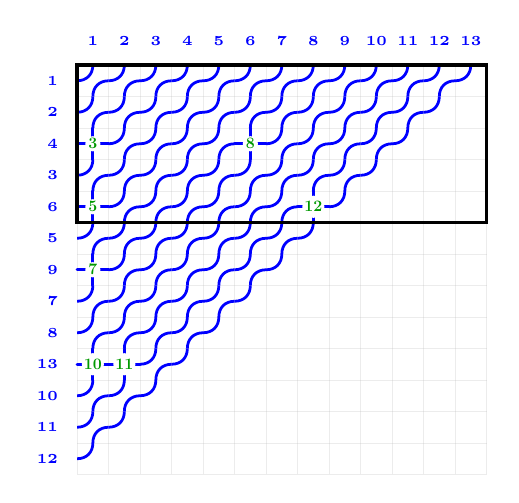
\begin{tikzpicture}[scale=0.4]
  \draw[lightgray, very thin, opacity=0.3] (13,0) -- (0,0);
  \draw[lightgray, very thin, opacity=0.3] (13,0) -- (13,13);
  \draw[lightgray, very thin, opacity=0.3] (13,1) -- (0,1);
  \draw[lightgray, very thin, opacity=0.3] (12,0) -- (12,13);
  \draw[lightgray, very thin, opacity=0.3] (13,2) -- (0,2);
  \draw[lightgray, very thin, opacity=0.3] (11,0) -- (11,13);
  \draw[lightgray, very thin, opacity=0.3] (13,3) -- (0,3);
  \draw[lightgray, very thin, opacity=0.3] (10,0) -- (10,13);
  \draw[lightgray, very thin, opacity=0.3] (13,4) -- (0,4);
  \draw[lightgray, very thin, opacity=0.3] (9,0) -- (9,13);
  \draw[lightgray, very thin, opacity=0.3] (13,5) -- (0,5);
  \draw[lightgray, very thin, opacity=0.3] (8,0) -- (8,13);
  \draw[lightgray, very thin, opacity=0.3] (13,6) -- (0,6);
  \draw[lightgray, very thin, opacity=0.3] (7,0) -- (7,13);
  \draw[lightgray, very thin, opacity=0.3] (13,7) -- (0,7);
  \draw[lightgray, very thin, opacity=0.3] (6,0) -- (6,13);
  \draw[lightgray, very thin, opacity=0.3] (13,8) -- (0,8);
  \draw[lightgray, very thin, opacity=0.3] (5,0) -- (5,13);
  \draw[lightgray, very thin, opacity=0.3] (13,9) -- (0,9);
  \draw[lightgray, very thin, opacity=0.3] (4,0) -- (4,13);
  \draw[lightgray, very thin, opacity=0.3] (13,10) -- (0,10);
  \draw[lightgray, very thin, opacity=0.3] (3,0) -- (3,13);
  \draw[lightgray, very thin, opacity=0.3] (13,11) -- (0,11);
  \draw[lightgray, very thin, opacity=0.3] (2,0) -- (2,13);
  \draw[lightgray, very thin, opacity=0.3] (13,12) -- (0,12);
  \draw[lightgray, very thin, opacity=0.3] (1,0) -- (1,13);
  \draw[lightgray, very thin, opacity=0.3] (13,13) -- (0,13);
  \draw[lightgray, very thin, opacity=0.3] (0,0) -- (0,13);
  \draw[blue, line width=1.0pt] (0,12.5) .. controls (0.3,12.5) and (0.5,12.7) .. (0.5,13);
  \draw[blue, line width=1.0pt] (0.5,12) .. controls (0.5,12.3) and (0.7,12.5) .. (1,12.5);
  \draw[blue, line width=1.0pt] (1,12.5) .. controls (1.3,12.5) and (1.5,12.7) .. (1.5,13);
  \draw[blue, line width=1.0pt] (1.5,12) .. controls (1.5,12.3) and (1.7,12.5) .. (2,12.5);
  \draw[blue, line width=1.0pt] (2,12.5) .. controls (2.3,12.5) and (2.5,12.7) .. (2.5,13);
  \draw[blue, line width=1.0pt] (2.5,12) .. controls (2.5,12.3) and (2.7,12.5) .. (3,12.5);
  \draw[blue, line width=1.0pt] (3,12.5) .. controls (3.3,12.5) and (3.5,12.7) .. (3.5,13);
  \draw[blue, line width=1.0pt] (3.5,12) .. controls (3.5,12.3) and (3.7,12.5) .. (4,12.5);
  \draw[blue, line width=1.0pt] (4,12.5) .. controls (4.3,12.5) and (4.5,12.7) .. (4.5,13);
  \draw[blue, line width=1.0pt] (4.5,12) .. controls (4.5,12.3) and (4.7,12.5) .. (5,12.5);
  \draw[blue, line width=1.0pt] (5,12.5) .. controls (5.3,12.5) and (5.5,12.7) .. (5.5,13);
  \draw[blue, line width=1.0pt] (5.5,12) .. controls (5.5,12.3) and (5.7,12.5) .. (6,12.5);
  \draw[blue, line width=1.0pt] (6,12.5) .. controls (6.3,12.5) and (6.5,12.7) .. (6.5,13);
  \draw[blue, line width=1.0pt] (6.5,12) .. controls (6.5,12.3) and (6.7,12.5) .. (7,12.5);
  \draw[blue, line width=1.0pt] (7,12.5) .. controls (7.3,12.5) and (7.5,12.7) .. (7.5,13);
  \draw[blue, line width=1.0pt] (7.5,12) .. controls (7.5,12.3) and (7.7,12.5) .. (8,12.5);
  \draw[blue, line width=1.0pt] (8,12.5) .. controls (8.3,12.5) and (8.5,12.7) .. (8.5,13);
  \draw[blue, line width=1.0pt] (8.5,12) .. controls (8.5,12.3) and (8.7,12.5) .. (9,12.5);
  \draw[blue, line width=1.0pt] (9,12.5) .. controls (9.3,12.5) and (9.5,12.7) .. (9.5,13);
  \draw[blue, line width=1.0pt] (9.5,12) .. controls (9.5,12.3) and (9.7,12.5) .. (10,12.5);
  \draw[blue, line width=1.0pt] (10,12.5) .. controls (10.3,12.5) and (10.5,12.7) .. (10.5,13);
  \draw[blue, line width=1.0pt] (10.5,12) .. controls (10.5,12.3) and (10.7,12.5) .. (11,12.5);
  \draw[blue, line width=1.0pt] (11,12.5) .. controls (11.3,12.5) and (11.5,12.7) .. (11.5,13);
  \draw[blue, line width=1.0pt] (11.5,12) .. controls (11.5,12.3) and (11.7,12.5) .. (12,12.5);
  \draw[blue, line width=1.0pt] (12,12.5) .. controls (12.3,12.5) and (12.5,12.7) .. (12.5,13);
  \draw[blue, line width=1.0pt] (0,11.5) .. controls (0.3,11.5) and (0.5,11.7) .. (0.5,12);
  \draw[blue, line width=1.0pt] (0.5,11) .. controls (0.5,11.3) and (0.7,11.5) .. (1,11.5);
  \draw[blue, line width=1.0pt] (1,11.5) .. controls (1.3,11.5) and (1.5,11.7) .. (1.5,12);
  \draw[blue, line width=1.0pt] (1.5,11) .. controls (1.5,11.3) and (1.7,11.5) .. (2,11.5);
  \draw[blue, line width=1.0pt] (2,11.5) .. controls (2.3,11.5) and (2.5,11.7) .. (2.5,12);
  \draw[blue, line width=1.0pt] (2.5,11) .. controls (2.5,11.3) and (2.7,11.5) .. (3,11.5);
  \draw[blue, line width=1.0pt] (3,11.5) .. controls (3.3,11.5) and (3.5,11.7) .. (3.5,12);
  \draw[blue, line width=1.0pt] (3.5,11) .. controls (3.5,11.3) and (3.7,11.5) .. (4,11.5);
  \draw[blue, line width=1.0pt] (4,11.5) .. controls (4.3,11.5) and (4.5,11.7) .. (4.5,12);
  \draw[blue, line width=1.0pt] (4.5,11) .. controls (4.5,11.3) and (4.7,11.5) .. (5,11.5);
  \draw[blue, line width=1.0pt] (5,11.5) .. controls (5.3,11.5) and (5.5,11.7) .. (5.5,12);
  \draw[blue, line width=1.0pt] (5.5,11) .. controls (5.5,11.3) and (5.7,11.5) .. (6,11.5);
  \draw[blue, line width=1.0pt] (6,11.5) .. controls (6.3,11.5) and (6.5,11.7) .. (6.5,12);
  \draw[blue, line width=1.0pt] (6.5,11) .. controls (6.5,11.3) and (6.7,11.5) .. (7,11.5);
  \draw[blue, line width=1.0pt] (7,11.5) .. controls (7.3,11.5) and (7.5,11.7) .. (7.5,12);
  \draw[blue, line width=1.0pt] (7.5,11) .. controls (7.5,11.3) and (7.7,11.5) .. (8,11.5);
  \draw[blue, line width=1.0pt] (8,11.5) .. controls (8.3,11.5) and (8.5,11.7) .. (8.5,12);
  \draw[blue, line width=1.0pt] (8.5,11) .. controls (8.5,11.3) and (8.7,11.5) .. (9,11.5);
  \draw[blue, line width=1.0pt] (9,11.5) .. controls (9.3,11.5) and (9.5,11.7) .. (9.5,12);
  \draw[blue, line width=1.0pt] (9.5,11) .. controls (9.5,11.3) and (9.7,11.5) .. (10,11.5);
  \draw[blue, line width=1.0pt] (10,11.5) .. controls (10.3,11.5) and (10.5,11.7) .. (10.5,12);
  \draw[blue, line width=1.0pt] (10.5,11) .. controls (10.5,11.3) and (10.7,11.5) .. (11,11.5);
  \draw[blue, line width=1.0pt] (11,11.5) .. controls (11.3,11.5) and (11.5,11.7) .. (11.5,12);
  \draw[blue, line width=1.0pt, line cap=round] (0,10.5) -- (1,10.5);
  \draw[blue, line width=1.0pt, line cap=round] (0.5,10) -- (0.5,11);
  \draw[blue, line width=1.0pt] (1,10.5) .. controls (1.3,10.5) and (1.5,10.7) .. (1.5,11);
  \draw[blue, line width=1.0pt] (1.5,10) .. controls (1.5,10.3) and (1.7,10.5) .. (2,10.5);
  \draw[blue, line width=1.0pt] (2,10.5) .. controls (2.3,10.5) and (2.5,10.7) .. (2.5,11);
  \draw[blue, line width=1.0pt] (2.5,10) .. controls (2.5,10.3) and (2.7,10.5) .. (3,10.5);
  \draw[blue, line width=1.0pt] (3,10.5) .. controls (3.3,10.5) and (3.5,10.7) .. (3.5,11);
  \draw[blue, line width=1.0pt] (3.5,10) .. controls (3.5,10.3) and (3.7,10.5) .. (4,10.5);
  \draw[blue, line width=1.0pt] (4,10.5) .. controls (4.3,10.5) and (4.5,10.7) .. (4.5,11);
  \draw[blue, line width=1.0pt] (4.5,10) .. controls (4.5,10.3) and (4.7,10.5) .. (5,10.5);
  \draw[blue, line width=1.0pt, line cap=round] (5,10.5) -- (6,10.5);
  \draw[blue, line width=1.0pt, line cap=round] (5.5,10) -- (5.5,11);
  \draw[blue, line width=1.0pt] (6,10.5) .. controls (6.3,10.5) and (6.5,10.7) .. (6.5,11);
  \draw[blue, line width=1.0pt] (6.5,10) .. controls (6.5,10.3) and (6.7,10.5) .. (7,10.5);
  \draw[blue, line width=1.0pt] (7,10.5) .. controls (7.3,10.5) and (7.5,10.7) .. (7.5,11);
  \draw[blue, line width=1.0pt] (7.5,10) .. controls (7.5,10.3) and (7.7,10.5) .. (8,10.5);
  \draw[blue, line width=1.0pt] (8,10.5) .. controls (8.3,10.5) and (8.5,10.7) .. (8.5,11);
  \draw[blue, line width=1.0pt] (8.5,10) .. controls (8.5,10.3) and (8.7,10.5) .. (9,10.5);
  \draw[blue, line width=1.0pt] (9,10.5) .. controls (9.3,10.5) and (9.5,10.7) .. (9.5,11);
  \draw[blue, line width=1.0pt] (9.5,10) .. controls (9.5,10.3) and (9.7,10.5) .. (10,10.5);
  \draw[blue, line width=1.0pt] (10,10.5) .. controls (10.3,10.5) and (10.5,10.7) .. (10.5,11);
  \draw[blue, line width=1.0pt] (0,9.5) .. controls (0.3,9.5) and (0.5,9.7) .. (0.5,10);
  \draw[blue, line width=1.0pt] (0.5,9) .. controls (0.5,9.3) and (0.7,9.5) .. (1,9.5);
  \draw[blue, line width=1.0pt] (1,9.5) .. controls (1.3,9.5) and (1.5,9.7) .. (1.5,10);
  \draw[blue, line width=1.0pt] (1.5,9) .. controls (1.5,9.3) and (1.7,9.5) .. (2,9.5);
  \draw[blue, line width=1.0pt] (2,9.5) .. controls (2.3,9.5) and (2.5,9.7) .. (2.5,10);
  \draw[blue, line width=1.0pt] (2.5,9) .. controls (2.5,9.3) and (2.7,9.5) .. (3,9.5);
  \draw[blue, line width=1.0pt] (3,9.5) .. controls (3.3,9.5) and (3.5,9.7) .. (3.5,10);
  \draw[blue, line width=1.0pt] (3.5,9) .. controls (3.5,9.3) and (3.7,9.5) .. (4,9.5);
  \draw[blue, line width=1.0pt] (4,9.5) .. controls (4.3,9.5) and (4.5,9.7) .. (4.5,10);
  \draw[blue, line width=1.0pt] (4.5,9) .. controls (4.5,9.3) and (4.7,9.5) .. (5,9.5);
  \draw[blue, line width=1.0pt] (5,9.5) .. controls (5.3,9.5) and (5.5,9.7) .. (5.5,10);
  \draw[blue, line width=1.0pt] (5.5,9) .. controls (5.5,9.3) and (5.7,9.5) .. (6,9.5);
  \draw[blue, line width=1.0pt] (6,9.5) .. controls (6.3,9.5) and (6.5,9.7) .. (6.5,10);
  \draw[blue, line width=1.0pt] (6.5,9) .. controls (6.5,9.3) and (6.7,9.5) .. (7,9.5);
  \draw[blue, line width=1.0pt] (7,9.5) .. controls (7.3,9.5) and (7.5,9.7) .. (7.5,10);
  \draw[blue, line width=1.0pt] (7.5,9) .. controls (7.5,9.3) and (7.7,9.5) .. (8,9.5);
  \draw[blue, line width=1.0pt] (8,9.5) .. controls (8.3,9.5) and (8.5,9.7) .. (8.5,10);
  \draw[blue, line width=1.0pt] (8.5,9) .. controls (8.5,9.3) and (8.7,9.5) .. (9,9.5);
  \draw[blue, line width=1.0pt] (9,9.5) .. controls (9.3,9.5) and (9.5,9.7) .. (9.5,10);
  \draw[blue, line width=1.0pt, line cap=round] (0,8.5) -- (1,8.5);
  \draw[blue, line width=1.0pt, line cap=round] (0.5,8) -- (0.5,9);
  \draw[blue, line width=1.0pt] (1,8.5) .. controls (1.3,8.5) and (1.5,8.7) .. (1.5,9);
  \draw[blue, line width=1.0pt] (1.5,8) .. controls (1.5,8.3) and (1.7,8.5) .. (2,8.5);
  \draw[blue, line width=1.0pt] (2,8.5) .. controls (2.3,8.5) and (2.5,8.7) .. (2.5,9);
  \draw[blue, line width=1.0pt] (2.5,8) .. controls (2.5,8.3) and (2.7,8.5) .. (3,8.5);
  \draw[blue, line width=1.0pt] (3,8.5) .. controls (3.3,8.5) and (3.5,8.7) .. (3.5,9);
  \draw[blue, line width=1.0pt] (3.5,8) .. controls (3.5,8.3) and (3.7,8.5) .. (4,8.5);
  \draw[blue, line width=1.0pt] (4,8.5) .. controls (4.3,8.5) and (4.5,8.7) .. (4.5,9);
  \draw[blue, line width=1.0pt] (4.5,8) .. controls (4.5,8.3) and (4.7,8.5) .. (5,8.5);
  \draw[blue, line width=1.0pt] (5,8.5) .. controls (5.3,8.5) and (5.5,8.7) .. (5.5,9);
  \draw[blue, line width=1.0pt] (5.5,8) .. controls (5.5,8.3) and (5.7,8.5) .. (6,8.5);
  \draw[blue, line width=1.0pt] (6,8.5) .. controls (6.3,8.5) and (6.5,8.7) .. (6.5,9);
  \draw[blue, line width=1.0pt] (6.5,8) .. controls (6.5,8.3) and (6.7,8.5) .. (7,8.5);
  \draw[blue, line width=1.0pt, line cap=round] (7,8.5) -- (8,8.5);
  \draw[blue, line width=1.0pt, line cap=round] (7.5,8) -- (7.5,9);
  \draw[blue, line width=1.0pt] (8,8.5) .. controls (8.3,8.5) and (8.5,8.7) .. (8.5,9);
  \draw[blue, line width=1.0pt] (0,7.5) .. controls (0.3,7.5) and (0.5,7.7) .. (0.5,8);
  \draw[blue, line width=1.0pt] (0.5,7) .. controls (0.5,7.3) and (0.7,7.5) .. (1,7.5);
  \draw[blue, line width=1.0pt] (1,7.5) .. controls (1.3,7.5) and (1.5,7.7) .. (1.5,8);
  \draw[blue, line width=1.0pt] (1.5,7) .. controls (1.5,7.3) and (1.7,7.5) .. (2,7.5);
  \draw[blue, line width=1.0pt] (2,7.5) .. controls (2.3,7.5) and (2.5,7.7) .. (2.5,8);
  \draw[blue, line width=1.0pt] (2.5,7) .. controls (2.5,7.3) and (2.7,7.5) .. (3,7.5);
  \draw[blue, line width=1.0pt] (3,7.5) .. controls (3.3,7.5) and (3.5,7.7) .. (3.5,8);
  \draw[blue, line width=1.0pt] (3.5,7) .. controls (3.5,7.3) and (3.7,7.5) .. (4,7.5);
  \draw[blue, line width=1.0pt] (4,7.5) .. controls (4.3,7.5) and (4.5,7.7) .. (4.5,8);
  \draw[blue, line width=1.0pt] (4.5,7) .. controls (4.5,7.3) and (4.7,7.5) .. (5,7.5);
  \draw[blue, line width=1.0pt] (5,7.5) .. controls (5.3,7.5) and (5.5,7.7) .. (5.5,8);
  \draw[blue, line width=1.0pt] (5.5,7) .. controls (5.5,7.3) and (5.7,7.5) .. (6,7.5);
  \draw[blue, line width=1.0pt] (6,7.5) .. controls (6.3,7.5) and (6.5,7.7) .. (6.5,8);
  \draw[blue, line width=1.0pt] (6.5,7) .. controls (6.5,7.3) and (6.7,7.5) .. (7,7.5);
  \draw[blue, line width=1.0pt] (7,7.5) .. controls (7.3,7.5) and (7.5,7.7) .. (7.5,8);
  \draw[blue, line width=1.0pt, line cap=round] (0,6.5) -- (1,6.5);
  \draw[blue, line width=1.0pt, line cap=round] (0.5,6) -- (0.5,7);
  \draw[blue, line width=1.0pt] (1,6.5) .. controls (1.3,6.5) and (1.5,6.7) .. (1.5,7);
  \draw[blue, line width=1.0pt] (1.5,6) .. controls (1.5,6.3) and (1.7,6.5) .. (2,6.5);
  \draw[blue, line width=1.0pt] (2,6.5) .. controls (2.3,6.5) and (2.5,6.7) .. (2.5,7);
  \draw[blue, line width=1.0pt] (2.5,6) .. controls (2.5,6.3) and (2.7,6.5) .. (3,6.5);
  \draw[blue, line width=1.0pt] (3,6.5) .. controls (3.3,6.5) and (3.5,6.7) .. (3.5,7);
  \draw[blue, line width=1.0pt] (3.5,6) .. controls (3.5,6.3) and (3.7,6.5) .. (4,6.5);
  \draw[blue, line width=1.0pt] (4,6.5) .. controls (4.3,6.5) and (4.5,6.7) .. (4.5,7);
  \draw[blue, line width=1.0pt] (4.5,6) .. controls (4.5,6.3) and (4.7,6.5) .. (5,6.5);
  \draw[blue, line width=1.0pt] (5,6.5) .. controls (5.3,6.5) and (5.5,6.7) .. (5.5,7);
  \draw[blue, line width=1.0pt] (5.5,6) .. controls (5.5,6.3) and (5.7,6.5) .. (6,6.5);
  \draw[blue, line width=1.0pt] (6,6.5) .. controls (6.3,6.5) and (6.5,6.7) .. (6.5,7);
  \draw[blue, line width=1.0pt] (0,5.5) .. controls (0.3,5.5) and (0.5,5.7) .. (0.5,6);
  \draw[blue, line width=1.0pt] (0.5,5) .. controls (0.5,5.3) and (0.7,5.5) .. (1,5.5);
  \draw[blue, line width=1.0pt] (1,5.5) .. controls (1.3,5.5) and (1.5,5.7) .. (1.5,6);
  \draw[blue, line width=1.0pt] (1.5,5) .. controls (1.5,5.3) and (1.7,5.5) .. (2,5.5);
  \draw[blue, line width=1.0pt] (2,5.5) .. controls (2.3,5.5) and (2.5,5.7) .. (2.5,6);
  \draw[blue, line width=1.0pt] (2.5,5) .. controls (2.5,5.3) and (2.7,5.5) .. (3,5.5);
  \draw[blue, line width=1.0pt] (3,5.5) .. controls (3.3,5.5) and (3.5,5.7) .. (3.5,6);
  \draw[blue, line width=1.0pt] (3.5,5) .. controls (3.5,5.3) and (3.7,5.5) .. (4,5.5);
  \draw[blue, line width=1.0pt] (4,5.5) .. controls (4.3,5.5) and (4.5,5.7) .. (4.5,6);
  \draw[blue, line width=1.0pt] (4.5,5) .. controls (4.5,5.3) and (4.7,5.5) .. (5,5.5);
  \draw[blue, line width=1.0pt] (5,5.5) .. controls (5.3,5.5) and (5.5,5.7) .. (5.5,6);
  \draw[blue, line width=1.0pt] (0,4.5) .. controls (0.3,4.5) and (0.5,4.7) .. (0.5,5);
  \draw[blue, line width=1.0pt] (0.5,4) .. controls (0.5,4.3) and (0.7,4.5) .. (1,4.5);
  \draw[blue, line width=1.0pt] (1,4.5) .. controls (1.3,4.5) and (1.5,4.7) .. (1.5,5);
  \draw[blue, line width=1.0pt] (1.5,4) .. controls (1.5,4.3) and (1.7,4.5) .. (2,4.5);
  \draw[blue, line width=1.0pt] (2,4.5) .. controls (2.3,4.5) and (2.5,4.7) .. (2.5,5);
  \draw[blue, line width=1.0pt] (2.5,4) .. controls (2.5,4.3) and (2.7,4.5) .. (3,4.5);
  \draw[blue, line width=1.0pt] (3,4.5) .. controls (3.3,4.5) and (3.5,4.7) .. (3.5,5);
  \draw[blue, line width=1.0pt] (3.5,4) .. controls (3.5,4.3) and (3.7,4.5) .. (4,4.5);
  \draw[blue, line width=1.0pt] (4,4.5) .. controls (4.3,4.5) and (4.5,4.7) .. (4.5,5);
  \draw[blue, line width=1.0pt, line cap=round] (0,3.5) -- (1,3.5);
  \draw[blue, line width=1.0pt, line cap=round] (0.5,3) -- (0.5,4);
  \draw[blue, line width=1.0pt, line cap=round] (1,3.5) -- (2,3.5);
  \draw[blue, line width=1.0pt, line cap=round] (1.5,3) -- (1.5,4);
  \draw[blue, line width=1.0pt] (2,3.5) .. controls (2.3,3.5) and (2.5,3.7) .. (2.5,4);
  \draw[blue, line width=1.0pt] (2.5,3) .. controls (2.5,3.3) and (2.7,3.5) .. (3,3.5);
  \draw[blue, line width=1.0pt] (3,3.5) .. controls (3.3,3.5) and (3.5,3.7) .. (3.5,4);
  \draw[blue, line width=1.0pt] (0,2.5) .. controls (0.3,2.5) and (0.5,2.7) .. (0.5,3);
  \draw[blue, line width=1.0pt] (0.5,2) .. controls (0.5,2.3) and (0.7,2.5) .. (1,2.5);
  \draw[blue, line width=1.0pt] (1,2.5) .. controls (1.3,2.5) and (1.5,2.7) .. (1.5,3);
  \draw[blue, line width=1.0pt] (1.5,2) .. controls (1.5,2.3) and (1.7,2.5) .. (2,2.5);
  \draw[blue, line width=1.0pt] (2,2.5) .. controls (2.3,2.5) and (2.5,2.7) .. (2.5,3);
  \draw[blue, line width=1.0pt] (0,1.5) .. controls (0.3,1.5) and (0.5,1.7) .. (0.5,2);
  \draw[blue, line width=1.0pt] (0.5,1) .. controls (0.5,1.3) and (0.7,1.5) .. (1,1.5);
  \draw[blue, line width=1.0pt] (1,1.5) .. controls (1.3,1.5) and (1.5,1.7) .. (1.5,2);
  \draw[blue, line width=1.0pt] (0,0.5) .. controls (0.3,0.5) and (0.5,0.7) .. (0.5,1);
  \node[font=\tiny\bfseries, text=blue, anchor=south] at (0.5,13.3) {1};
  \node[font=\tiny\bfseries, text=blue, anchor=south] at (1.5,13.3) {2};
  \node[font=\tiny\bfseries, text=blue, anchor=south] at (2.5,13.3) {3};
  \node[font=\tiny\bfseries, text=blue, anchor=south] at (3.5,13.3) {4};
  \node[font=\tiny\bfseries, text=blue, anchor=south] at (4.5,13.3) {5};
  \node[font=\tiny\bfseries, text=blue, anchor=south] at (5.5,13.3) {6};
  \node[font=\tiny\bfseries, text=blue, anchor=south] at (6.5,13.3) {7};
  \node[font=\tiny\bfseries, text=blue, anchor=south] at (7.5,13.3) {8};
  \node[font=\tiny\bfseries, text=blue, anchor=south] at (8.5,13.3) {9};
  \node[font=\tiny\bfseries, text=blue, anchor=south] at (9.5,13.3) {10};
  \node[font=\tiny\bfseries, text=blue, anchor=south] at (10.5,13.3) {11};
  \node[font=\tiny\bfseries, text=blue, anchor=south] at (11.5,13.3) {12};
  \node[font=\tiny\bfseries, text=blue, anchor=south] at (12.5,13.3) {13};
  \node[font=\tiny\bfseries, text=blue, anchor=east] at (-0.3,12.5) {1};
  \node[font=\tiny\bfseries, text=blue, anchor=east] at (-0.3,11.5) {2};
  \node[font=\tiny\bfseries, text=blue, anchor=east] at (-0.3,10.5) {4};
  \node[font=\tiny\bfseries, text=blue, anchor=east] at (-0.3,9.5) {3};
  \node[font=\tiny\bfseries, text=blue, anchor=east] at (-0.3,8.5) {6};
  \node[font=\tiny\bfseries, text=blue, anchor=east] at (-0.3,7.5) {5};
  \node[font=\tiny\bfseries, text=blue, anchor=east] at (-0.3,6.5) {9};
  \node[font=\tiny\bfseries, text=blue, anchor=east] at (-0.3,5.5) {7};
  \node[font=\tiny\bfseries, text=blue, anchor=east] at (-0.3,4.5) {8};
  \node[font=\tiny\bfseries, text=blue, anchor=east] at (-0.3,3.5) {13};
  \node[font=\tiny\bfseries, text=blue, anchor=east] at (-0.3,2.5) {10};
  \node[font=\tiny\bfseries, text=blue, anchor=east] at (-0.3,1.5) {11};
  \node[font=\tiny\bfseries, text=blue, anchor=east] at (-0.3,0.5) {12};
  \draw[black, line width=1.2000000000000002pt] (13,8) rectangle (0,13);
  \node[font=\Large\bfseries, text=green!60!black, fill=white, inner sep=0.5pt, circle, transform shape] at (0.5,10.5) {3};
  \node[font=\Large\bfseries, text=green!60!black, fill=white, inner sep=0.5pt, circle, transform shape] at (5.5,10.5) {8};
  \node[font=\Large\bfseries, text=green!60!black, fill=white, inner sep=0.5pt, circle, transform shape] at (0.5,8.5) {5};
  \node[font=\Large\bfseries, text=green!60!black, fill=white, inner sep=0.5pt, circle, transform shape] at (7.5,8.5) {12};
  \node[font=\Large\bfseries, text=green!60!black, fill=white, inner sep=0.5pt, circle, transform shape] at (0.5,6.5) {7};
  \node[font=\Large\bfseries, text=green!60!black, fill=white, inner sep=0.5pt, circle, transform shape] at (0.5,3.5) {10};
  \node[font=\Large\bfseries, text=green!60!black, fill=white, inner sep=0.5pt, circle, transform shape] at (1.5,3.5) {11};
\end{tikzpicture}
} \\
$(R_1)$ & $(R_2)$
\end{tabular}
\caption{The two $10$-row witness pipe dreams in the forest class for $c$.}
\label{fig:forest_lr_witnesses}
\end{figure}

\begin{figure}[h]
\centering
\begin{tabular}{cc}
\resizebox{0.35\textwidth}{!}{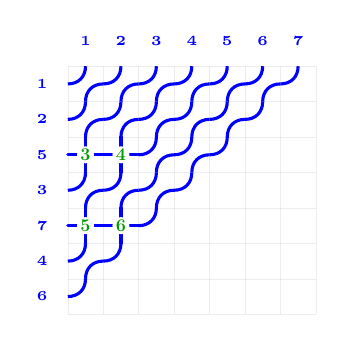
\begin{tikzpicture}[scale=0.45]
  \draw[lightgray, very thin, opacity=0.3] (7,0) -- (0,0);
  \draw[lightgray, very thin, opacity=0.3] (7,0) -- (7,7);
  \draw[lightgray, very thin, opacity=0.3] (7,1) -- (0,1);
  \draw[lightgray, very thin, opacity=0.3] (6,0) -- (6,7);
  \draw[lightgray, very thin, opacity=0.3] (7,2) -- (0,2);
  \draw[lightgray, very thin, opacity=0.3] (5,0) -- (5,7);
  \draw[lightgray, very thin, opacity=0.3] (7,3) -- (0,3);
  \draw[lightgray, very thin, opacity=0.3] (4,0) -- (4,7);
  \draw[lightgray, very thin, opacity=0.3] (7,4) -- (0,4);
  \draw[lightgray, very thin, opacity=0.3] (3,0) -- (3,7);
  \draw[lightgray, very thin, opacity=0.3] (7,5) -- (0,5);
  \draw[lightgray, very thin, opacity=0.3] (2,0) -- (2,7);
  \draw[lightgray, very thin, opacity=0.3] (7,6) -- (0,6);
  \draw[lightgray, very thin, opacity=0.3] (1,0) -- (1,7);
  \draw[lightgray, very thin, opacity=0.3] (7,7) -- (0,7);
  \draw[lightgray, very thin, opacity=0.3] (0,0) -- (0,7);
  \draw[blue, line width=1.125pt] (0,6.5) .. controls (0.3,6.5) and (0.5,6.7) .. (0.5,7);
  \draw[blue, line width=1.125pt] (0.5,6) .. controls (0.5,6.3) and (0.7,6.5) .. (1,6.5);
  \draw[blue, line width=1.125pt] (1,6.5) .. controls (1.3,6.5) and (1.5,6.7) .. (1.5,7);
  \draw[blue, line width=1.125pt] (1.5,6) .. controls (1.5,6.3) and (1.7,6.5) .. (2,6.5);
  \draw[blue, line width=1.125pt] (2,6.5) .. controls (2.3,6.5) and (2.5,6.7) .. (2.5,7);
  \draw[blue, line width=1.125pt] (2.5,6) .. controls (2.5,6.3) and (2.7,6.5) .. (3,6.5);
  \draw[blue, line width=1.125pt] (3,6.5) .. controls (3.3,6.5) and (3.5,6.7) .. (3.5,7);
  \draw[blue, line width=1.125pt] (3.5,6) .. controls (3.5,6.3) and (3.7,6.5) .. (4,6.5);
  \draw[blue, line width=1.125pt] (4,6.5) .. controls (4.3,6.5) and (4.5,6.7) .. (4.5,7);
  \draw[blue, line width=1.125pt] (4.5,6) .. controls (4.5,6.3) and (4.7,6.5) .. (5,6.5);
  \draw[blue, line width=1.125pt] (5,6.5) .. controls (5.3,6.5) and (5.5,6.7) .. (5.5,7);
  \draw[blue, line width=1.125pt] (5.5,6) .. controls (5.5,6.3) and (5.7,6.5) .. (6,6.5);
  \draw[blue, line width=1.125pt] (6,6.5) .. controls (6.3,6.5) and (6.5,6.7) .. (6.5,7);
  \draw[blue, line width=1.125pt] (0,5.5) .. controls (0.3,5.5) and (0.5,5.7) .. (0.5,6);
  \draw[blue, line width=1.125pt] (0.5,5) .. controls (0.5,5.3) and (0.7,5.5) .. (1,5.5);
  \draw[blue, line width=1.125pt] (1,5.5) .. controls (1.3,5.5) and (1.5,5.7) .. (1.5,6);
  \draw[blue, line width=1.125pt] (1.5,5) .. controls (1.5,5.3) and (1.7,5.5) .. (2,5.5);
  \draw[blue, line width=1.125pt] (2,5.5) .. controls (2.3,5.5) and (2.5,5.7) .. (2.5,6);
  \draw[blue, line width=1.125pt] (2.5,5) .. controls (2.5,5.3) and (2.7,5.5) .. (3,5.5);
  \draw[blue, line width=1.125pt] (3,5.5) .. controls (3.3,5.5) and (3.5,5.7) .. (3.5,6);
  \draw[blue, line width=1.125pt] (3.5,5) .. controls (3.5,5.3) and (3.7,5.5) .. (4,5.5);
  \draw[blue, line width=1.125pt] (4,5.5) .. controls (4.3,5.5) and (4.5,5.7) .. (4.5,6);
  \draw[blue, line width=1.125pt] (4.5,5) .. controls (4.5,5.3) and (4.7,5.5) .. (5,5.5);
  \draw[blue, line width=1.125pt] (5,5.5) .. controls (5.3,5.5) and (5.5,5.7) .. (5.5,6);
  \draw[blue, line width=1.125pt, line cap=round] (0,4.5) -- (1,4.5);
  \draw[blue, line width=1.125pt, line cap=round] (0.5,4) -- (0.5,5);
  \draw[blue, line width=1.125pt, line cap=round] (1,4.5) -- (2,4.5);
  \draw[blue, line width=1.125pt, line cap=round] (1.5,4) -- (1.5,5);
  \draw[blue, line width=1.125pt] (2,4.5) .. controls (2.3,4.5) and (2.5,4.7) .. (2.5,5);
  \draw[blue, line width=1.125pt] (2.5,4) .. controls (2.5,4.3) and (2.7,4.5) .. (3,4.5);
  \draw[blue, line width=1.125pt] (3,4.5) .. controls (3.3,4.5) and (3.5,4.7) .. (3.5,5);
  \draw[blue, line width=1.125pt] (3.5,4) .. controls (3.5,4.3) and (3.7,4.5) .. (4,4.5);
  \draw[blue, line width=1.125pt] (4,4.5) .. controls (4.3,4.5) and (4.5,4.7) .. (4.5,5);
  \draw[blue, line width=1.125pt] (0,3.5) .. controls (0.3,3.5) and (0.5,3.7) .. (0.5,4);
  \draw[blue, line width=1.125pt] (0.5,3) .. controls (0.5,3.3) and (0.7,3.5) .. (1,3.5);
  \draw[blue, line width=1.125pt] (1,3.5) .. controls (1.3,3.5) and (1.5,3.7) .. (1.5,4);
  \draw[blue, line width=1.125pt] (1.5,3) .. controls (1.5,3.3) and (1.7,3.5) .. (2,3.5);
  \draw[blue, line width=1.125pt] (2,3.5) .. controls (2.3,3.5) and (2.5,3.7) .. (2.5,4);
  \draw[blue, line width=1.125pt] (2.5,3) .. controls (2.5,3.3) and (2.7,3.5) .. (3,3.5);
  \draw[blue, line width=1.125pt] (3,3.5) .. controls (3.3,3.5) and (3.5,3.7) .. (3.5,4);
  \draw[blue, line width=1.125pt, line cap=round] (0,2.5) -- (1,2.5);
  \draw[blue, line width=1.125pt, line cap=round] (0.5,2) -- (0.5,3);
  \draw[blue, line width=1.125pt, line cap=round] (1,2.5) -- (2,2.5);
  \draw[blue, line width=1.125pt, line cap=round] (1.5,2) -- (1.5,3);
  \draw[blue, line width=1.125pt] (2,2.5) .. controls (2.3,2.5) and (2.5,2.7) .. (2.5,3);
  \draw[blue, line width=1.125pt] (0,1.5) .. controls (0.3,1.5) and (0.5,1.7) .. (0.5,2);
  \draw[blue, line width=1.125pt] (0.5,1) .. controls (0.5,1.3) and (0.7,1.5) .. (1,1.5);
  \draw[blue, line width=1.125pt] (1,1.5) .. controls (1.3,1.5) and (1.5,1.7) .. (1.5,2);
  \draw[blue, line width=1.125pt] (0,0.5) .. controls (0.3,0.5) and (0.5,0.7) .. (0.5,1);
  \node[font=\tiny\bfseries, text=blue, anchor=south] at (0.5,7.3) {1};
  \node[font=\tiny\bfseries, text=blue, anchor=south] at (1.5,7.3) {2};
  \node[font=\tiny\bfseries, text=blue, anchor=south] at (2.5,7.3) {3};
  \node[font=\tiny\bfseries, text=blue, anchor=south] at (3.5,7.3) {4};
  \node[font=\tiny\bfseries, text=blue, anchor=south] at (4.5,7.3) {5};
  \node[font=\tiny\bfseries, text=blue, anchor=south] at (5.5,7.3) {6};
  \node[font=\tiny\bfseries, text=blue, anchor=south] at (6.5,7.3) {7};
  \node[font=\tiny\bfseries, text=blue, anchor=east] at (-0.3,6.5) {1};
  \node[font=\tiny\bfseries, text=blue, anchor=east] at (-0.3,5.5) {2};
  \node[font=\tiny\bfseries, text=blue, anchor=east] at (-0.3,4.5) {5};
  \node[font=\tiny\bfseries, text=blue, anchor=east] at (-0.3,3.5) {3};
  \node[font=\tiny\bfseries, text=blue, anchor=east] at (-0.3,2.5) {7};
  \node[font=\tiny\bfseries, text=blue, anchor=east] at (-0.3,1.5) {4};
  \node[font=\tiny\bfseries, text=blue, anchor=east] at (-0.3,0.5) {6};
  \node[font=\Large\bfseries, text=green!60!black, fill=white, inner sep=0.5pt, circle, transform shape] at (0.5,4.5) {3};
  \node[font=\Large\bfseries, text=green!60!black, fill=white, inner sep=0.5pt, circle, transform shape] at (1.5,4.5) {4};
  \node[font=\Large\bfseries, text=green!60!black, fill=white, inner sep=0.5pt, circle, transform shape] at (0.5,2.5) {5};
  \node[font=\Large\bfseries, text=green!60!black, fill=white, inner sep=0.5pt, circle, transform shape] at (1.5,2.5) {6};
\end{tikzpicture}
} &
\resizebox{0.35\textwidth}{!}{\input{forest_lr_trim.tikz}} \\
$\clp^5(R_i)$ & $\trm^5(R_i)$
\end{tabular}
\caption{Common clip/trim pair for both witnesses $R_1,R_2$.}
\label{fig:forest_lr_cliptrim}
\end{figure}

Therefore Theorem~\ref{theorem:LRforest} gives
$$f_{a,b}^c=2.$$ 
\end{example}


% $$\dsch_u = [\code_1(u)]\dsch_{\downarrow u} - \sum_{\substack{u'\downvar{1} \downarrow u\\ \ell(\downarrow u,u')=\code_1(u)\\u'\neq u}}\dsch_{u'}$$
% where $\downarrow u$ is the unique permutation such that $\code_i(\downarrow u) = \code_{i+1}(u)$.


\begin{corollary}[Dual forest coproduct]\label{corollary:dforestcoproduct}
Let $c$ be a weak composition of length $n$, and let $\beta_{ab}^c$ denote the structure constants of forest polynomial multiplication, $\forest_a\forest_b=\sum_c\beta_{ab}^c\,\forest_c$ in $\coma_n$; these are nonnegative integers \cite{nadeau2024forest,bergeron2025equivariant}, and an enumerative Littlewood--Richardson rule for them is proved in the companion paper \cite{companionforest}. Then in $\dcoma_n\otimes\dcoma_n$,
$$\Delta^*(\forest_c^*) \;=\; \sum_{a,b}\beta_{ab}^c\,\forest_a^*\otimes\forest_b^*.$$
In particular, the dual forest coproduct has nonnegative integer structure constants in the dual forest basis, and these are exactly the forest polynomial Littlewood--Richardson coefficients.
\end{corollary}
\begin{proof}
Exactly as in the proof of Theorem~\ref{theorem:dschcoproduct}, pairing the expansion $\Delta^*(\forest_c^*) = \sum_{a,b}\lambda_{a,b}\forest_a^*\otimes\forest_b^*$ with $\forest_a\otimes\forest_b$ and using the defining identity $\langle\Delta^*(\alpha),x\otimes y\rangle = \langle \alpha, xy\rangle$ together with the duality $\langle \forest_a^*,\forest_b\rangle = \delta_{a,b}$ yields
$$\lambda_{a,b}\;=\;\langle \forest_c^*,\forest_a\forest_b\rangle\;=\;\langle \forest_c^*,\textstyle\sum_{c'}\beta_{ab}^{c'}\forest_{c'}\rangle\;=\;\beta_{ab}^c.$$
\end{proof}

\subsubsection*{Branching comorphism on the quasisymmetric flag variety}\label{subsection:qflbranch}

The dual forest LR rule (Theorem~\ref{theorem:LRforest}) admits a geometric reading on the quasisymmetric flag variety $\mathrm{QFl}_n$ of Bergeron--Gagnon--Nadeau--Spink--Tewari \cite{bergeron2025qsymflag}, a toric subcomplex of $\mathrm{Fl}_n$ stratified by translated Richardson varieties $X(F)$ indexed by indexed forests. Using the Borel-type presentation $H^\bullet(\mathrm{QFl}_n)\cong \mathbb{Z}[x_1,\ldots,x_n]/\mathrm{QSym}_n^+$ \cite[Theorem~A and Corollary~12.5]{bergeron2025qsymflag}, the variable-splitting substitution
$$\rho_{p,q}:\;\mathbb{Z}[x_1,\ldots,x_{p+q}]\longrightarrow \mathbb{Z}[x_1,\ldots,x_p]\otimes \mathbb{Z}[x_{p+1},\ldots,x_{p+q}]$$
descends to a well-defined ring homomorphism
$$\iota_{p,q}^*:\;H^\bullet(\mathrm{QFl}_{p+q})\longrightarrow H^\bullet(\mathrm{QFl}_p)\otimes H^\bullet(\mathrm{QFl}_q).$$
Indeed, for $f\in\mathrm{QSym}_{p+q}^+$ the standard alphabet-sum identity for the QSym coproduct writes $\rho_{p,q}(f) = \sum f_{(1)}(x_1,\ldots,x_p)\otimes f_{(2)}(x_{p+1},\ldots,x_{p+q})$ with each $f_{(1)}$, $f_{(2)}$ quasisymmetric in its variables; since $\deg f>0$ and the degrees add, each term has at least one tensor factor in $\mathrm{QSym}^+$, so $\rho_{p,q}(f)\in \mathrm{QSym}_p^+\otimes\mathbb{Z}[y] + \mathbb{Z}[x]\otimes \mathrm{QSym}_q^+$. The splitting reformulation of Theorem~\ref{theorem:LRforest} then says exactly that, in the forest-polynomial basis,
$$\iota_{p,q}^*\,[\forest_c] \;=\; \sum_{a,b} f_{a,b}^c\;[\forest_a]\otimes [\forest_b]\qquad\text{in } H^\bullet(\mathrm{QFl}_p)\otimes H^\bullet(\mathrm{QFl}_q),$$
and Theorem~\ref{theorem:LRforest} gives an explicit positive cardinality formula for each $f_{a,b}^c$.

The map $\iota_{p,q}^*$ is the natural quasisymmetric-flag analogue of the type-A Levi comorphism $H^\bullet(\mathrm{Fl}_{p+q})\to H^\bullet(\mathrm{Fl}_p)\otimes H^\bullet(\mathrm{Fl}_q)$ of \cite{ressayre2009branching}, and the dual forest LR rule plays for it the role that Theorem~\ref{theorem:LR} plays for the Schubert basis. We do not know whether $\iota_{p,q}^*$ is induced by a geometric embedding $\mathrm{QFl}_p\times \mathrm{QFl}_q\hookrightarrow \mathrm{QFl}_{p+q}$ compatible with the Levi inclusion $\mathrm{Fl}_p\times \mathrm{Fl}_q\hookrightarrow \mathrm{Fl}_{p+q}$; the natural concatenation operation $\mathsf{Forest}_p\times \mathsf{Forest}_q\to \mathsf{Forest}_{p+q}$ on indexed forests, and the resulting matching $X(F)\times X(F')\subset \mathrm{QFl}_{p+q}$ one expects on the toric Richardson side, suggest that such an embedding should exist, but we do not pursue the geometric verification here. At the level of cohomology rings $\iota_{p,q}^*$ is in any case a well-defined ring homomorphism, and Theorem~\ref{theorem:LRforest} is, in this language, a manifestly positive branching Schubert calculus rule on the quasisymmetric flag variety, parallel to the one Theorem~\ref{theorem:LR} provides on $\mathrm{Fl}_n$. Dually, the family $\{\iota_{p,q}^*\}_{p,q\geq 0}$ assembles into a graded coproduct on $\bigoplus_n H_\bullet(\mathrm{QFl}_n)$ whose structure constants in the geometric forest basis $\{[X(F)]\}$ are again the $f_{a,b}^c$ of Theorem~\ref{theorem:LRforest}.


\section{Product rule for dual slide polynomials}\label{section:slide}
\subsection{Slide polynomials}

\begin{definition}
For a word $\mathbf{r}=\mathbf{r}_1\mathbf{r}_2\cdots \mathbf{r}_k$, a sequence of positive integers $a_1a_2\cdots a_k$ is \emph{compatible} with $\mathbf{r}$ if $a_i\leq \mathbf{r}_i$ for all $i$, $a_i\leq a_{i+1}$ for all $i$, and $a_i<a_{i+1}$ if $\mathbf{r}_i<\mathbf{r}_{i+1}$.

Slide polynomials $\mathfrak{F}(\mathbf{r})$ for a word $\mathbf{r}$ are defined by summing the monomials $x^a$ over all compatible sequences $a$ of $\mathbf{r}$.

Assaf and Searles \cite{assaf2017slide} derived an expansion of Schubert polynomials in terms of slide polynomials as follows. A \emph{quasi-Yamanouchi} RC graph is an RC graph $R$ such that if $R'$ is another RC graph with $\mathrm{word}(R)=\mathrm{word}(R')$ and $\hr(R)=\hr(R')$, then $\wtt(R)\leq \wtt(R')$ in dominance order and $\mathrm{flat}(\wtt(R'))$ refines $\mathrm{flat}(\wtt(R))$. The set of RC graphs $A$ such that $\mathrm{word}(A)=\mathrm{word}(R)$ and $\hr(A)=\hr(R)$ is a partially ordered set with $R$ as its smallest element. We then define
$$\QY(A)=R$$
\end{definition}

\begin{theorem}[{\cite[Theorem~3.13]{assaf2017slide}}]
  For a permutation $w\in S_\infty$, we have the formula
  $$\sch_w(x) = \sum_{R} \mathfrak{F}_{\wtt(R)}(x)$$
  where the sum is over all quasi-Yamanouchi RC graphs $R$ for $w$.
\end{theorem}
% \section{Recursion for Schubert structure constants}
\begin{corollary}
  For a weak composition $c$ of length $p$, we have the formula
  $$\mathfrak{F}_c^* = \sum_{R=\QY(R)} \dsch_{\wof{R}}^p$$
  where the sum is over all quasi-Yamanouchi RC graphs $R$ such that $\wtt(R) = c$.
\end{corollary}


\begin{remark}
The expansion of dual slides in the weak composition basis is given by the expansion of monomials into slides in \cite[Theorem~5.2]{nadeau2024ppartitions}.
\end{remark}

\begin{definition}[The submodule $\Sigma\subseteq \BRC$]
Let $\Sigma$ be the $\mathbb{Z}$-submodule of $\BRC$ generated by the elements $R_1-R_2$ such that $\QY(R_1)=\QY(R_2)$.
\end{definition}

By the definition of $\QY$, the relation $\QY(R_1)=\QY(R_2)$ holds precisely when $R_1$ and $R_2$ have the same word and the same height, since $\QY(R)$ is by construction the least element of the poset of RC graphs $A$ with $\mathrm{word}(A)=\mathrm{word}(R)$ and $\hr(A)=\hr(R)$. We use this description of the generators of $\Sigma$ throughout; it is also the description recorded in Remark \ref{remark:general_lr_instances}.

\begin{lemma}\label{lemma:slideideal}
$\Sigma$ is a two-sided ideal of $\BRC$.
\end{lemma}
\begin{proof}
Since RC graphs with the same word have the same permutation, $\Sigma\subseteq\Omega$ and Lemma \ref{lemma:blockdecomp} and Corollary \ref{corollary:blockswap} apply.

\emph{Left ideal.} Let $A$ have $\hr(A)=k$ and let $R_1-R_2$ be a generator of $\Sigma$ with $\hr(R_j)=m$, so $\mathrm{word}(R_1)=\mathrm{word}(R_2)$. By Corollary \ref{corollary:blockswap} the terms of $A\sqcupplus R_1$ and $A\sqcupplus R_2$ are matched by $A'\cup\shup^{k}R_1\leftrightarrow A'\cup\shup^{k}R_2$, and corresponding terms have words $\mathrm{word}(A')\cdot(\mathrm{word}(R_j)+k)$. These coincide, so the matched terms have the same word and the same height, whence their difference lies in $\Sigma$.

\emph{Right ideal.} Let $A$ have $\hr(A)=k$. Since $\wof{R_1}=\wof{R_2}$, Lemma \ref{lemma:topmatch} supplies the bijection $\beta$ matching the terms of $R_1\sqcupplus A$ with those of $R_2\sqcupplus A$, corresponding terms having words $\mathrm{word}(B)\cdot(\mathrm{word}(A)+m)$ and $\mathrm{word}(\beta(B))\cdot(\mathrm{word}(A)+m)$. It therefore suffices to show $\mathrm{word}(B)=\mathrm{word}(\beta(B))$, and by Lemma \ref{lemma:topmatch}(3) it is enough to treat a single application of $\zeromap$. So suppose $\zeromap(B)=R_1$ and $\zeromap(\beta(B))=R_2$ with $\wof B=\wof{\beta(B)}$. By Proposition \ref{proposition:zerocrystal} and Proposition \ref{proposition:little_bump}, $\mathrm{word}(B)$ is determined by $\mathrm{word}(R_1)$ together with $\wof B$, since the passage from $B$ to $\zeromap(B)$ is a sequence of Little bumps whose starting position is determined by the permutation. As $\mathrm{word}(R_1)=\mathrm{word}(R_2)$ and $\wof B=\wof{\beta(B)}$, we get $\mathrm{word}(B)=\mathrm{word}(\beta(B))$, so $(R_1-R_2)\sqcupplus A\in\Sigma$.
\end{proof}

\begin{lemma}
The homomorphism $\alpha:\BRC\to\dcoma$ factors through the quotient $\BRC/\Sigma$.
\end{lemma}
\begin{proof}
This is because the generators of $\Sigma$ are all in $\Omega$: if $\QY(R_1)=\QY(R_2)$ then $\wof{R_1}=\wof{\QY(R_1)}=\wof{\QY(R_2)}=\wof{R_2}$ and $\hr(R_1)=\hr(R_2)$, so $\alpha(R_1)=\alpha(R_2)$.
\end{proof}

\begin{definition}
For a weak composition $a$, define an element $\mathcal{F}_a\in\BRC/\Sigma$ by
$$\mathcal{F}_a=\sum_{R: \QY(R)=R,\ \wtt(R)=a} R.$$
\end{definition}

\begin{proposition}\label{proposition:slidebasis}
The elements $\mathcal{F}_a\in\BRC/\Sigma$ form an additive basis of a subring isomorphic to $\dcoma$ under the homomorphism $\alpha:\BRC/\Sigma\to\dcoma$, and
$$\alpha(\mathcal{F}_a)=\mathfrak{F}_a^*.$$
\end{proposition}
\begin{proof}
The last identity is the Corollary above. Distinct $\mathcal{F}_a$ are supported on disjoint sets of quasi-Yamanouchi RC graphs (indexed by their common weight $a$), so the $\mathcal{F}_a$ are linearly independent in $\BRC/\Sigma$. Considering the homomorphism $\alpha:\BRC/\Sigma\to\dcoma$, since the $\mathfrak{F}_a^*$ are linearly independent, the kernel of $\alpha$ intersects the span of the $\mathcal{F}_a$ trivially; hence $\alpha$ is injective on $\sum_a \mathbb{Z}\mathcal{F}_a$. Since
$$\alpha(\mathcal{F}_a)\sqcupplus\alpha(\mathcal{F}_b)=\mathfrak{F}_a^*\sqcupplus\mathfrak{F}_b^*=\sum_c s_{a,b}^c\,\mathfrak{F}_c^*=\sum_c s_{a,b}^c\,\alpha(\mathcal{F}_c),$$
the product $\mathcal{F}_a\sqcupplus\mathcal{F}_b$ lies in the span of the $\mathcal{F}_c$, so this span is closed under multiplication and the restriction of $\alpha$ is a ring isomorphism.
\end{proof}

\begin{theorem} \label{theorem:lrfslide}
  Let $a,b$ be weak compositions of lengths $p$ and $q$. Write
$$\mathfrak{F}_a^*\sqcupplus\mathfrak{F}_b^*=\sum_c s_{a,b}^c\,\mathfrak{F}_c^*$$
For each $c$, fix an RC graph $C$ with $\wtt(\QY(C)) = c$. Then $s_{a,b}^c$ is the number of distinct RC graphs $R$ with $\mathrm{word}(R)=\mathrm{word}(C)$ with $\wtt(\clp^p(R)) = a,\wtt(\trm^p(R)) = b$ such that $\clp^p(R),\trm^p(R)$ are quasi-Yamanouchi, and is in particular nonnegative.
\end{theorem}
\begin{proof}
The coefficient of $\mathcal{F}_c$ in $\mathcal{F}_a\sqcupplus\mathcal{F}_b$ equals the coefficient of $\mathfrak{F}_c^*$ in $\mathfrak{F}_a^*\sqcupplus\mathfrak{F}_b^*$, namely $s_{a,b}^c$, by Proposition \ref{proposition:slidebasis}. Expanding the product $\mathcal{F}_a\sqcupplus\mathcal{F}_b$ via the $(\clp^p,\trm^p)$-decomposition of $\sqcupplus$ (Theorem \ref{theorem:modactrc}) and reading off the coefficient of $\mathcal{F}_c$ from a fixed representative $C$ with $\wtt(\QY(C))=c$, the contributing terms are precisely the RC graphs $R$ with $\mathrm{word}(R)=\mathrm{word}(C)$ whose clip and trim have quasi-Yamanouchi weights $a$ and $b$ respectively.
\end{proof}

\subsection{A general ideal-quotient Littlewood--Richardson principle}

The dual Schubert, dual key, and dual forest LR rules of the previous sections all fit a common template, which we record here.

\begin{theorem}[General LR principle via ideals of $\BRC$]\label{theorem:general_lr_template}
Let $\sim$ be an equivalence relation on $\bigsqcup_n \RC_n$ satisfying:
\begin{itemize}
\item[(H1)] If $R_1\sim R_2$ then $\hr(R_1)=\hr(R_2)$ and $\wof{R_1}=\wof{R_2}$ (in particular $\alpha(R_1)=\alpha(R_2)$).
\item[(H2)] $\sim$ is a congruence for $\sqcupplus$: $R_1\sim R_2$ implies $R\sqcupplus R_1\sim R\sqcupplus R_2$ and $R_1\sqcupplus R\sim R_2\sqcupplus R$ for every $R$.
\item[(H3)] $\clp^p$ and $\trm^p$ descend to $\sim$: if $R_1\sim R_2$ and $1\leq p\leq \hr(R_1)$, then $\clp^p(R_1)\sim \clp^p(R_2)$ and $\trm^p(R_1)\sim \trm^p(R_2)$.
\item[(H4)] There is an index set $J$ and a function $\lambda:(\RC/\!\sim)\to J$ such that, writing $I_\sim=\mathrm{span}_{\mathbb{Z}}\{R_1-R_2:R_1\sim R_2\}\subseteq\BRC$ and
$$E_\lambda := \sum_{[R]:\,\lambda([R])=\lambda} [R] \in \BRC/I_\sim,$$
the family $\{\alpha(E_\lambda)\}_{\lambda\in J}$ is a $\mathbb{Z}$-basis of $\dcoma$.

\end{itemize}
Then $I_\sim$ is a two-sided ideal of $\BRC$ contained in $\Omega=\ker\alpha$, the elements $\{E_\lambda\}$ span a subring of $\BRC/I_\sim$ isomorphic to $\dcoma$ via $\alpha$, and the structure constants $b_{\mu,\nu}^\lambda$ defined by
$$\mathfrak{B}_\mu^*\sqcupplus\mathfrak{B}_\nu^* = \sum_\lambda b_{\mu,\nu}^\lambda\,\mathfrak{B}_\lambda^*,\qquad \mathfrak{B}_\lambda^*:=\alpha(E_\lambda),$$
are nonnegative integers. More precisely, for any function $\mathrm{rep}\colon\RC\to\RC$ that sends every element of a $\sim$-class to a single common representative of that class (that is, $\mathrm{rep}(R)\sim R$ for all $R$, and $\mathrm{rep}(R)=\mathrm{rep}(S)$ whenever $R\sim S$), we have the positive combinatorial formula
\begin{align*}
b_{\mu,\nu}^\lambda \;=\; \#\bigl\{\,R\sim C\ :\ &\clp^p(R)=\mathrm{rep}(\clp^p(R)),\;\;\trm^p(R)=\mathrm{rep}(\trm^p(R)),\\
&\lambda([\clp^p(R)])=\mu,\;\;\lambda([\trm^p(R)])=\nu\,\bigr\}
\end{align*}
for any fixed $C$ with $\lambda([C])=\lambda$. The count is independent of the choice of $\mathrm{rep}$.
\end{theorem}
\begin{proof}
By (H1) every generator $R_1-R_2$ of $I_\sim$ lies in $\Omega=\ker\alpha$, so $I_\sim\subseteq\Omega$ and $\alpha$ descends to a surjective ring homomorphism $\overline\alpha:\BRC/I_\sim\to\dcoma$. By (H2), $I_\sim$ is a two-sided ideal of $\BRC$, so $\BRC/I_\sim$ inherits a ring structure.

By construction of $E_\lambda$ in (H4), each $\sim$-class $[R]$ appears in $E_\lambda$ with multiplicity exactly $1$ (when $\lambda([R])=\lambda$) or $0$ (otherwise), and the supports of $E_\lambda$ and $E_{\lambda'}$ in $\BRC/I_\sim$ are disjoint whenever $\lambda\neq\lambda'$; consequently the coefficient $b_{\mu,\nu}^\lambda$ may be read off from the contribution to a single chosen class $[C]$ with $\lambda([C])=\lambda$. In particular the $\{E_\lambda\}$ are linearly independent. Under $\overline\alpha$ they map to the $\mathbb{Z}$-basis $\{\mathfrak{B}_\lambda^*\}$ of $\dcoma$ by (H4), so $\overline\alpha$ restricts to a $\mathbb{Z}$-module isomorphism $\bigoplus_\lambda\mathbb{Z}E_\lambda\xrightarrow{\;\cong\;}\dcoma$. Since $\overline\alpha$ is a ring homomorphism, the span of the $E_\lambda$ is closed under multiplication and the isomorphism is one of rings. Consequently
$$E_\mu \sqcupplus E_\nu = \sum_\lambda b_{\mu,\nu}^\lambda\, E_\lambda \quad\text{in } \BRC/I_\sim.$$

To read off $b_{\mu,\nu}^\lambda$, fix any $C$ with $\lambda([C])=\lambda$ and let $S_1=\mathrm{rep}(R_1)$, $S_2=\mathrm{rep}(R_2)$ be the chosen representatives of the $\mu$- and $\nu$-classes (for any $R_1,R_2$ in those classes). By Theorem~\ref{theorem:modactrc} the product $\sqcupplus$ on $\BRC$ admits a $(\clp^p,\trm^p)$-decomposition: for any $S_1,S_2$ with $\hr(S_1)=p$, $\hr(S_2)=q$, the set $\{R\in\RC_{p+q}:\clp^p(R)=S_1,\,\trm^p(R)=S_2\}$ enumerates the summands of $S_1\sqcupplus S_2$ with multiplicity one. Projecting to $\BRC/I_\sim$, (H3) ensures that the class of $R$ depends only on the classes of $\clp^p(R)$ and $\trm^p(R)$, so the contribution of $S_1\sqcupplus S_2$ to the coefficient of $[C]$ in $E_\lambda$ is exactly the count of $R\sim C$ for which $\clp^p(R)=S_1$ and $\trm^p(R)=S_2$, i.e.\ for which $\clp^p(R)$ and $\trm^p(R)$ are themselves fixed points of $\mathrm{rep}$ and represent the $\mu$- and $\nu$-classes. This is the stated formula. Being a cardinality, it is nonnegative.

Finally, the count is independent of the choice of $\mathrm{rep}$. The element $E_\lambda\in\BRC/I_\sim$ is defined directly as $\sum_{[R]:\lambda([R])=\lambda}[R]$, with no reference to $\mathrm{rep}$, so the structure constants in $E_\mu E_\nu=\sum_\lambda b_{\mu,\nu}^\lambda E_\lambda$ are intrinsic. To see that the formula computes the correct value for every valid $\mathrm{rep}$, fix classes $[T_1],[T_2]$ with $\lambda([T_1])=\mu$, $\lambda([T_2])=\nu$, and consider, for any $S_1\in[T_1]$ and $S_2\in[T_2]$, the count
$$N(S_1,S_2):=\#\{R\sim C\,:\,\clp^p(R)=S_1,\ \trm^p(R)=S_2\}.$$
By the $(\clp^p,\trm^p)$-decomposition of Theorem~\ref{theorem:modactrc}, $N(S_1,S_2)$ equals the coefficient of $[C]$ in the product $[S_1]\sqcupplus[S_2]\in\BRC/I_\sim$ (using (H2) to make the product well-defined and (H3) to ensure each summand of $S_1\sqcupplus S_2$ has $\sim$-class depending only on $[S_1]$ and $[S_2]$). In particular $N(S_1,S_2)$ depends only on the classes $[T_1],[T_2]$ and on $[C]$, not on the choice of representatives $S_1,S_2$. The $\mathrm{rep}$-formula selects, for each such class-pair, the single representative pair $(\mathrm{rep}(T_1),\mathrm{rep}(T_2))$ and counts $N(\mathrm{rep}(T_1),\mathrm{rep}(T_2))$; another valid $\mathrm{rep}'$ counts $N(\mathrm{rep}'(T_1),\mathrm{rep}'(T_2))$, and these are equal. Summing over class-pairs yields the same total $b_{\mu,\nu}^\lambda$.
\end{proof}

\begin{remark}\label{remark:general_lr_instances}
In the present paper, Theorem~\ref{theorem:general_lr_template} is instantiated by
\begin{itemize}
\item $\sim$ = equality on $\RC$, with $I_\sim=0$ and $\lambda([R])=(\wof{R},\hr(R))$, recovering Theorem~\ref{theorem:LR} (dual Schubert basis);
\item $\sim$ = Demazure-crystal equivalence, with $I_\sim=\Theta$ and $\lambda$ the extremal weight, recovering Theorem~\ref{theorem:LRkey} (dual key basis);
\item $\sim\,=\,\equiv_\forest$, with $I_\sim=\Gamma$ and $\lambda=\fcode$, recovering Theorem~\ref{theorem:LRforest} (dual forest basis);
\item $\sim$ = ``same reduced word and same $\hr$'' on $\RC$, with $\lambda([R])=\wtt(\QY(R))$, recovering Theorem~\ref{theorem:lrfslide} (dual slide basis).
\end{itemize}
The verifications of (H1)--(H4) in each case are precisely the lemmas and propositions of \S\ref{section:bialgebra}, \S\ref{section:crystals}, \S\ref{section:forest}, and \S\ref{section:slide}.
\end{remark}


\section*{Notation and conventions}\label{section:notation}

For the reader's convenience we collect here, in one place, the principal symbols used throughout the article. All notation is introduced in context where it is needed; this list is meant as a navigational aid rather than a definition.

\begingroup
\setlist[description]{
  font=\normalfont,
  leftmargin=2em,
  labelindent=0em,
  labelsep=0.5em,
  itemsep=2pt,
  parsep=0pt,
  topsep=4pt,
}

\subsubsection*{Permutations and combinatorial objects}
\begin{description}
\item[$S_\infty$] The group of permutations of $\mathbb{Z}_{>0}$ fixing all but finitely many elements.
\item[$\ell(w)$] The Coxeter length of $w\in S_\infty$.
\item[$\code(w)$, $\code^*(w)$] The (right) Lehmer code of $w$; the code of $w^{-1}$.
\item[$\maxd(w)$] The position of the last descent of $w$.
\item[$\dom_\lambda$] The dominant permutation with $\code^*(\dom_\lambda)=\lambda$.
\item[$\mathsf{IndexedForests}_n$] The set of indexed forests on $[n]$ in the sense of Nadeau--Tewari \cite{nadeau2024forest}; matched bijectively with $\mathrm{Comp}_n$ via $F\leftrightarrow\code(F)$, so we use $a\in\mathrm{Comp}_n$ and $F_a\in\mathsf{IndexedForests}_n$ interchangeably.
\item[$\mathsf{Forest}_n$] The subset of $\mathsf{IndexedForests}_n$ corresponding to the homology basis $\{[X(F)]\}$ of $H_\bullet(\mathrm{QFl}_n)$ in BGNST \cite[Cor.~11.6]{bergeron2025qsymflag}; in NST language, those $F$ with $n\notin\mathrm{LT}(F)$.
\item[$\mathsf{Tree}_n$] The set of $n$-leaf planar binary trees, identified with the irreducible components of $\mathrm{QFl}_n$.
\item[$\RC_n$] The set of bounded RC graphs with $n$ rows (Definition~\ref{definition:rcgraph}).
\item[$\RC_n(w)$] The set of $R\in\RC_n$ with $\wof{R}=w$.
\item[$\RC_n^0$] The set of $R\in\RC_n$ whose last row is empty (\S\ref{section:brc}).
\item[$\wof{R}$] The permutation of an RC graph $R$.
\item[$\hr(R)$] The number of rows of $R$.
\item[$\wtt(R)$] The row weight composition of $R$.
\item[$\mathrm{word}(R)$] The reduced word read from $R$.
\end{description}

\subsubsection*{Row maps on RC graphs}
\begin{description}
\item[$\zeromap$] The transition map $\RC_n^0\to\RC_{n-1}$ of Definition~\ref{definition:zeromap}; it realizes the Lascoux--Sch\"utzenberger transition formula on the last row.
\item[$\trm^p(R)$] ``Truncate'': the RC graph obtained from the last $\hr(R)-p$ rows of $R$ (\S\ref{section:ringproduct}).
\item[$\clp^p(R)$] ``Clip'': the RC graph in $\RC_p$ obtained from $R$ by an insertion algorithm based on $\zeromap$; the dual partner of $\trm^p$ (\S\ref{section:ringproduct}).
\item[$\shup^p$] Shift indices up by $p$ (applied to permutations or letters).
\end{description}

\subsubsection*{Crystal and forest structures}
\begin{description}
\item[$e_i,f_i$] Crystal raising and lowering operators on RC graphs (Definition~\ref{definition:crystal}).
\item[$\mathrm{Dem}(R)$] The Demazure crystal of $R$ (Assaf--Schilling; Definition~\ref{definition:crystal}).
\item[$\mathrm{Dem}_a$] $\{R:\mathrm{extwt}(R)=a\}$, the set of RC graphs with extremal weight $a$ (\S\ref{section:crystals}).
\item[$\mathrm{extwt}(R)$] The extremal weight of $\mathrm{Dem}(R)$, i.e.\ the weight of its unique lowest weight element (Definition~\ref{definition:crystal}).
\item[$\mathbb{Y}(R)$] The highest-weight representative of $R$ in its Demazure crystal (Definition~\ref{definition:crystal}).
\item[$\mathbb{Y}_\forest(R)$] The forest analog of $\mathbb{Y}(R)$: the canonical representative of $R$ in its forest equivalence class, used in the dual forest LR rule (\S\ref{section:forest}).
\item[$\finv(R)$] The forest invariant of $R$, an indexed forest (Nadeau--Tewari; \S\ref{section:forest}).
\item[$\fcode(R)\,(=\code_\forest(R))$] The composition associated to $\finv(R)$ (\S\ref{section:forest}). The forms $\fcode(R)$ and $\code_\forest(R)$ are used interchangeably.
\item[$\mathcal{C}_\forest(a)$] The set of forest classes of RC graphs with $\fcode=a$ (\S\ref{section:forest}).
\item[$\equiv_\forest$] Forest equivalence: $R\equiv_\forest R'$ iff $\finv(R)=\finv(R')$ (\S\ref{section:forest}).
\item[$\RC_\forest(c)$] The set of $R\in\RC_n$ with $\wtt(R)=c$ such that $\mathrm{word}(\mathbb{Y}_\forest(R))$ is lex-minimal among $R'$ with $\code_\forest(R')=\code_\forest(R)$ (Theorem~\ref{theorem:forestformula}).
\end{description}

\subsubsection*{The Schubert bialgebra and its dual}
\begin{description}
\item[$\coma_n$] The polynomial ring $\mathbb{Z}[x_1,\ldots,x_n]$ (\S\ref{section:bialgebra}).
\item[$\coma$] The Schubert bialgebra $\bigoplus_{n\geq 0}\coma_n$, with $\coma_m\cdot\coma_n=0$ when $m\neq n>0$ (\S\ref{section:bialgebra}).
\item[$\dcoma$] The graded dual bialgebra of $\coma$ (\S\ref{section:dualalgebra}).
\item[$\sch_u^n$] Schubert polynomial in $\coma_n$, $\maxd(u)\leq n$ (\S\ref{section:bialgebra}).
\item[$\dsch_u^n$] Element of $\dcoma$ dual to $\sch_u^n$ (\S\ref{section:dualalgebra}).
\item[$\mathrm{ev}$] The evaluation map $\BRC\to\coma$ defined by $\mathrm{ev}(R)=x^{\wtt(R)}$ on basis elements (\S\ref{section:brc}).
\item[$\kappa_a$, $\kappa_a^*$] Key polynomial / its dual; $a\in\mathrm{Comp}_n$ (\S\ref{section:crystals}).
\item[$\forest_a$, $\forest_a^*$] Forest polynomial / its dual; $a\in\mathrm{Comp}_n$ (\S\ref{section:forest}).
\item[{$x_a$, $[a]$, $e_{\mathbf b}$}] The monomial $x^{a}=x_1^{a_1}\cdots x_n^{a_n}\in\coma_n$; its dual basis element in $\dcoma_n$, written either $[a]$ or $e_{\mathbf b}$ depending on context.
\item[$\langle -,-\rangle$] The bialgebra pairing $\dcoma\otimes\coma\to\mathbb{Z}$ defined by $\langle [a],x^{b}\rangle=\delta_{a,b}$, equivalently $\langle e_{\mathbf a},x^{\mathbf b}\rangle=\delta_{\mathbf a,\mathbf b}$.
\item[$\mathrm{Comp}_n$] The set of weak compositions of length $n$.
\item[$\Delta$, $\nabla$, $\varepsilon$] Coproduct, product, counit on $\coma$ (\S\ref{section:bialgebra}).
\item[$\Delta^*$] The dual coproduct on $\dcoma$, dual to the polynomial product on $\coma$ (\S\ref{section:dualalgebra}).
\end{description}

\subsubsection*{Structure constants}
\begin{description}
\item[$c_{u,v}^w$] Schubert structure constants: $\sch_u\sch_v=\sum c_{u,v}^w\sch_w$.
\item[$d_{u,v}^w(p,q)$] Dual Schubert structure constants of Theorem~\ref{theorem:LR}.
\item[$k_{a,b}^c$] Dual key structure constants of Theorem~\ref{theorem:LRkey}.
\item[$f_{a,b}^c$] Dual forest structure constants of Theorem~\ref{theorem:LRforest}.
\item[$s_{a,b}^c$] Dual slide structure constants of Theorem~\ref{theorem:lrfslide}.
\item[$\beta_{ab}^c$] The forest polynomial LR coefficients: $\forest_a\,\forest_b=\sum_c\beta_{ab}^c\,\forest_c$ in $\coma_n$; equivalently, the structure constants of $\Delta^*$ in the dual forest basis (Corollary~\ref{corollary:dforestcoproduct}). An enumerative rule is given in the companion paper \cite{companionforest}.
\item[$b_{\mu,\nu}^\lambda$] The general dual LR structure constants of Theorem~\ref{theorem:general_lr_template}.
\end{description}

\subsubsection*{The ring of RC graphs and its quotients}
\begin{description}
\item[$\BRC$] $\bigoplus_{n\geq 0}\mathbb{Z}^{\oplus\RC_n}$, with the product $\sqcupplus$ (\S\ref{section:brc}).
\item[$\BRC_n$] The graded component $\mathbb{Z}^{\oplus \RC_n}$ of $\BRC$ (RC graphs of height exactly $n$).
\item[$\mathcal{S}_w(n)$] $\sum_{R:\,\wof{R}=w,\,\hr(R)=n}R\in\BRC_n$, the sum of all $n$-row RC graphs of permutation $w$; satisfies $\alpha(\mathcal{S}_w(n))=\dsch_w^n$ and $\mathrm{ev}(\mathcal{S}_w(n))=\sch_w^n$ (\S\ref{section:brc}).
\item[$K_a$] $\sum_{R\in\mathrm{Dem}_a,\,R=\mathbb{Y}(R)} R\in\BRC/\Theta$, the dual key class sum; $\alpha(K_a)=\kappa_a^*$ (\S\ref{section:crystals}).
\item[$F_a$] $\sum_{[R]\in\mathcal{C}_\forest(a)}[R]\in\BRC/\Gamma$, the dual forest class sum; $\alpha(F_a)=\forest_a^*$ (\S\ref{section:forest}).
\item[$\sqcupplus$] The associative concatenation product on $\BRC$, on $\dcoma$, and on the quotients $\BRC/I_\sim$; built from $\clp^p$ and $\trm^p$ on $\BRC$ (\S\ref{section:ringproduct}).
\item[$\alpha:\BRC\to\dcoma$] Ring homomorphism with $\alpha(R)=\dsch_{\wof{R}}^{\hr(R)}$ (\S\ref{section:brc}).
\item[$\Omega$] $\ker\alpha$, the two-sided ideal of $\BRC$ on which $\alpha$ vanishes (Definition~\ref{definition:omega}; Theorem~\ref{theorem:semidirect}).
\item[$\Theta$] The two-sided ideal generated by $R_1-R_2$ with $\mathbb{Y}(R_1)=\mathbb{Y}(R_2)$ (Definition~\ref{definition:theta}); $\BRC/\Theta$ supports the dual key LR rule (Theorem~\ref{theorem:LRkey}).
\item[$\Gamma$] The two-sided ideal generated by $R_1-R_2$ with $R_1\equiv_\forest R_2$ (Definition~\ref{definition:gamma}); $\BRC/\Gamma$ supports the dual forest LR rule (Theorem~\ref{theorem:LRforest}).
\item[$\mathcal{E}_n$] The elementary basis of $\coma_n$ (Theorem~\ref{theorem:elemtrans}).
\end{description}

\subsubsection*{Slide polynomials and the general LR template}
\begin{description}
\item[$\mathfrak{F}_a(x)$, $\mathfrak{F}_a^*$] Slide polynomial in $\coma$ (Assaf--Searles) indexed by a weak composition $a$; its dual in $\dcoma$ (\S\ref{section:slide}).
\item[$\QY(R)$] Quasi-Yamanouchi representative of $R$ in its $(\mathrm{word},\hr)$-class; smallest element under the dominance/refinement order on weights (\S\ref{section:slide}).
\item[$\RC_\QY(c)$] Set of RC graphs $R$ with $\wtt(R)=c$ such that $\mathrm{word}(\QY(R))$ is lex-minimal among $R'$ with $\wtt(\QY(R'))=\wtt(\QY(R))$ (\S\ref{section:slide}).
\item[$\Sigma$] Two-sided ideal of $\BRC$ generated by $R_1-R_2$ with $\QY(R_1)=\QY(R_2)$ (Lemma~\ref{lemma:slideideal}).
\item[$\mathcal{F}_a$] The element $\sum_{R=\QY(R),\,\wtt(R)=a} R\in\BRC/\Sigma$, a representative of the slide basis under $\alpha$ (Proposition~\ref{proposition:slidebasis}).
\item[$\sim$] A generic equivalence relation on $\bigsqcup_n\RC_n$ satisfying (H1)--(H4) of Theorem~\ref{theorem:general_lr_template}.
\item[$I_\sim$] The two-sided ideal $\mathrm{span}_{\mathbb{Z}}\{R_1-R_2:R_1\sim R_2\}\subseteq\BRC$ (Theorem~\ref{theorem:general_lr_template}).
\item[$J$, $\lambda$] Index set, resp.\ labeling map $(\RC/\!\sim)\to J$ in the general LR template (Theorem~\ref{theorem:general_lr_template}).
\item[$E_\lambda$] The class sum $\sum_{[R]:\,\lambda([R])=\lambda}[R]\in\BRC/I_\sim$ (Theorem~\ref{theorem:general_lr_template}).
\item[$\mathfrak{B}_\lambda^*$, $b_{\mu,\nu}^\lambda$] Image $\alpha(E_\lambda)\in\dcoma$ and the corresponding structure constants in Theorem~\ref{theorem:general_lr_template}.
\end{description}

\subsubsection*{Quasisymmetric flag variety (\S\ref{subsection:qflbranch})}
\begin{description}
\item[$\mathrm{QFl}_n$] The quasisymmetric flag variety of Bergeron--Gagnon--Nadeau--Spink--Tewari \cite{bergeron2025qsymflag}, a toric subcomplex of $\mathrm{Fl}_n$ stratified by $X(F)$ for $F\in\mathsf{Forest}_n$.
\item[{$X(F)$, $[X(F)]$}] The toric Richardson variety attached to $F\in\mathsf{Forest}_n$, and its homology class; $\{[X(F)]\}$ is a $\mathbb{Z}$-basis of $H_\bullet(\mathrm{QFl}_n)$ \cite[Cor.~11.6]{bergeron2025qsymflag}.
\item[$H^\bullet(\mathrm{QFl}_n)$, $H_\bullet(\mathrm{QFl}_n)$] Cohomology and homology of $\mathrm{QFl}_n$, paired by the integration map $\int_{X(F)}(\cdot)$.
\item[$\mathrm{QSym}_n^+$] The ideal of quasisymmetric polynomials in $\mathbb{Z}[x_1,\ldots,x_n]$ with no constant term; $\mathrm{QSym}_n^+\!\cdot\coma_n$ is the kernel of the Borel surjection.
\item[$\pi_n$] The Borel-type surjection $\coma_n\twoheadrightarrow\coma_n/(\mathrm{QSym}_n^+\!\cdot\coma_n)\cong H^\bullet(\mathrm{QFl}_n)$ \cite[Thm.~A and Cor.~12.5]{bergeron2025qsymflag}.
\item[{$[\forest_a]$}] The cohomology class $\pi_n(\forest_a)\in H^\bullet(\mathrm{QFl}_n)$; under the Borel isomorphism, $\{[\forest_a]:F_a\in\mathsf{Forest}_n\}$ is a $\mathbb{Z}$-basis of $H^\bullet(\mathrm{QFl}_n)$, Kronecker dual to $\{[X(F_a)]\}$.
\item[$\rho_{p,q}$, $\iota_{p,q}^*$] The variable-splitting substitution $\coma_{p+q}\to\coma_p\otimes\coma_q$, and the induced ring homomorphism
$$H^\bullet(\mathrm{QFl}_{p+q})\to H^\bullet(\mathrm{QFl}_p)\otimes H^\bullet(\mathrm{QFl}_q)$$
(\S\ref{subsection:qflbranch}).
\item[$\epsilon_F(\mathbf{b})$] The path sign of \cite[Prop.~10.15]{nadeau2024quasisymmetric}: the coefficient of $\forest_F$ in the forest expansion of $x^{\mathbf{b}}$, valued in $\{-1,0,+1\}$. By Proposition~\ref{proposition:forestdualcoefficients}, $\langle\forest_a^*,x^{\mathbf{b}}\rangle=\epsilon_{F_a}(\mathbf{b})$.
\item[$V_F(\boldsymbol\lambda)$] The volume polynomial of \cite[\S 10.5]{nadeau2024quasisymmetric}, dual to $\forest_F$ under the divided-power $D$-pairing; $V_F(\boldsymbol\lambda)=\sum_{\mathbf{b}}\epsilon_F(\mathbf{b})\,\boldsymbol\lambda^{\mathbf{b}}/\mathbf{b}!$.
\end{description}
\endgroup

\appendix
\section{Proof of Proposition \ref{proposition:pullindex}}


\renewcommand{\theproposition2}{\Alph{proposition2}}
\setcounter{lemma}{0}

We dedicate this section to the otherwise distracting proof of Proposition \ref{proposition:pullindex}.

\begin{proposition2}[Special case of Pieri formula {\cite[Theorem~7.1]{samuelmolev}}] \label{proposition:pieri}
Suppose $k\geq 1$ and $u,w\in S_\infty$. If $u\not\tom{k} w$, then
$$\ddv{y}_u^w\prod_{i=1}^k(x_1 - y_i)=0$$
If $u\tom{k} w$, define
$$Q = \{u(i)\mid i\leq k\mbox{ and }u(i)=w(i)\}$$
then
$$\ddv{y}_u^w\prod_{i=1}^k(x_1 - y_i)=\prod_{q\in Q}(x_1 - y_q)$$
\end{proposition2}
\begin{proof}
	To avoid confusion, we point out that the original theorem is stated on the $x$ variables, whereas this theorem is in terms of the $y$ variables. Besides this, this is a restatement of the cited theorem in the special case of $p=k$, that is to say the Molev-Sagan Pieri formula for double Schubert polynomials.
\end{proof}

\begin{proof}[Proof of Proposition \ref{proposition:pullindex}]
Suppose $v\in S_n$. We have
$$\sch_v(x;y)=\ddv{y}^{vw_0(n)}(\sch_{w_0(n)}(x;y))$$
This is equal to
$$\ddv{y}^{vw_0(n)}\left(\sch_{s_{n+1-i}\cdots s_1w_0(n)}(x^{(i)};y)\prod_{j=1}^{n+1-i}(x_i - y_j)\right)$$
and, applying the Leibniz formula, is also equal to
$$\sum_{\substack{v'\in S_\infty\\\ell(v'w_0(n)s_1\cdots s_{n+1-i})\\=\ell(w_0(n)s_1\cdots s_{n+1-i})-\ell(v')}}\sch_{v'}(x^{(i)};y)\ddv{y}_{v'w_0(n)s_1\cdots s_{n+1-i}}^{vw_0(n)}\prod_{j=1}^{n+1-i}(x_i - y_j)$$
By the restricted Pieri formula (Proposition \ref{proposition:pieri}), for this to be nonzero we need $v'w_0(n)s_1\cdots s_{n+1-i}\allowbreak\tom{n+1-i}vw_0(n)$. We note that $v'w_0(n)s_1\cdots s_{n+1-i}\tom{n+1-i}vw_0(n)$ if and only if 
$$v\Tom{i}v'w_0(n)s_1\cdots s_{n+1-i}w_0(n)=v's_ns_{n-1}\cdots s_i$$
We have that $v's_n\cdots s_i$ is exactly $\varphi_{i,n}(v')$ since $v'\in S_n$, so we require that
$$v\Tom{i}\varphi_{i,n}(v')$$
so the sum is over all $v'$ with $v\downvar{i} v'$.

Applying Proposition \ref{proposition:pieri}, we obtain that the result is equal to
$$\sum_{v\downvar{i} v'} \sch_{v'}(x^{(i)};y)\prod_{a\in A(v',v)}(x_i - y_a)$$
where $A(v',v)$ is the set of all $vw_0(n)(j)$ such that $1\leq j\leq n+1-i$ and $v'w_0(n)s_1\cdots s_{n+1-i}(j)=vw_0(n)(j)$. These values are the same as at the indices that comprise the set of all $1\leq j\leq n+1-i$ such that
$$v'(n+2-s_1\cdots s_{n+1-i}(j))=v(n+2-j)$$
Applying the $s_1\cdots s_{n+1-i}$ to $j$, since $1\leq j\leq n+1-i$ we have that 
$$s_1\cdots s_{n+1-i}(j)=j+1$$
Hence we need
$$v'(n+2-(j+1))=v'(n+1-j)=v(n+2-j)$$
Replacing $j$ with $n+2-p$, the indices are the set of all $p$ such that $i<p\leq n+1$ and
$$v'(p-1)=v(p)$$
Thus $A(v',v)$ is the set of all $v(p)$ such that $p>i$ and $v'(p-1)=v(p)$, which is exactly $Q_i(v',v)$, and we are done.
\end{proof}

\section*{Acknowledgements}

The author is deeply grateful to Zachary Hamaker for many illuminating conversations during the development of this work, and in particular for introducing the author to forest polynomials in the first place, in addition to pointing out the connections of RC graph crystal operators to  Little's bumping algorithm. Thanks are also due to Frank Sottile, whose work, much of it now classical, has been a sustained guiding influence on the author's thinking about Schubert calculus, and whose generosity with his time over the years has shaped the perspective taken here.

\bibliographystyle{acm}
\bibliography{schubert_bialgebra}


\end{document}